\documentclass[final,subfig,blackref]{drexel-thesis}

\usepackage{amsmath}
\usepackage{amssymb}
\usepackage{textcomp}
\usepackage{tabu}
\usepackage{multirow}
\usepackage{enumitem}
\usepackage{rotating}
\usepackage{xspace}

\usepackage{natbib}
\bibliographystyle{aasjournal}

\newcommand{\hMpc}{$h^{-1}$Mpc\xspace}
\newcommand{\OH}{$12 + \log(\text{O}/\text{H})$}
\newcommand{\NH}{$12 + \log(\text{N}/\text{H})$}
\newcommand{\NO}{$\log(\text{N}/\text{O})$}
\newcommand{\RA}[4]{{#1}$^\text{h}${#2}$^\text{m}${#3}$^\text{s}${#4}}
\newcommand{\dec}[4]{{#1}\textdegree {#2}'{#3}''{#4}}

\makeatletter
\newcommand{\ion}[2]{{#1} \expandafter\@slowromancap\romannumeral #2@}
\makeatother


\author{Kelly A. Douglass}
\title{Observational evidence of the large-scale environmental influence on dwarf galaxy evolution}
\DUTmonth{July}
\DUTyear{2017}
\degree{Doctor of Philosophy}
\advisor{Dr. Michael S. Vogeley}
\copyrighttext{}


\begin{document}

% Preamble
\begin{preamble}

\iffinal{}{\newpage}

%%%%%%%%%%%%%%%%%%%%%%%%%%%%%%%%%%%%%%%%%%%%%%%%%%%%%%%%%%%%%%%%%%%%%%%%%%%%%%%%
% Dedications
%%%%%%%%%%%%%%%%%%%%%%%%%%%%%%%%%%%%%%%%%%%%%%%%%%%%%%%%%%%%%%%%%%%%%%%%%%%%%%%%

\begin{DUTdedications}
\begin{center}
Dedications
\end{center}
\end{DUTdedications}

\iffinal{}{\newpage}

%%%%%%%%%%%%%%%%%%%%%%%%%%%%%%%%%%%%%%%%%%%%%%%%%%%%%%%%%%%%%%%%%%%%%%%%%%%%%%%%
% Acknowledgements
%%%%%%%%%%%%%%%%%%%%%%%%%%%%%%%%%%%%%%%%%%%%%%%%%%%%%%%%%%%%%%%%%%%%%%%%%%%%%%%%

\begin{acknowledgments}

I would like to thank Crystal Moorman for her help and support throughout this 
work.  I would also like to acknowledge Renyue Cen for his help in the 
interpretation of these results.  Finally, I would like to thank the referees 
(including Burcu Beygu) for their detailed comments and critique of my work.

Support for this work was provided by NSF grant AST--1410525.

Funding for the SDSS and SDSS-II has been provided by the Alfred P. Sloan 
Foundation, the Participating Institutions, the National Science Foundation, the 
U.S. Department of Energy, the National Aeronautics and Space Administration, 
the Japanese Monbukagakusho, the Max Planck Society, and the Higher Education 
Funding Council for England.  The SDSS Web Site is \emph{http://www.sdss.org/}.

The SDSS is managed by the Astrophysical Research Consortium for the 
Participating Institutions.  The Participating Institutions are the American 
Museum of Natural History, Astrophysical Institute Potsdam, University of Basil, 
University of Cambridge, Case Western Reserve University, University of Chicago, 
Drexel University, Fermilab, the Institute for Advanced Study, the Japan 
Participation Group, Johns Hopkins University, the Joint Institute for Nuclear 
Astrophysics, the Kavli Institute for Particle Astrophysics and Cosmology, the 
Korean Scientist Group, the Chinese Academy of Sciences (LAMOST), Los Alamos 
National Laboratory, the Max-Planck-Institute for Astronomy (MPIA), the 
Max-Planck-Institute for Astrophysics (MPA), New Mexico State University, Ohio 
State University, University of Pittsburgh, University of Portsmouth, Princeton 
University, the United States Naval Observatory, and the University of 
Washington.

\end{acknowledgments}

\iffinal{}{\newpage}

%%%%%%%%%%%%%%%%%%%%%%%%%%%%%%%%%%%%%%%%%%%%%%%%%%%%%%%%%%%%%%%%%%%%%%%%%%%%%%%%
% Table of Contents
%%%%%%%%%%%%%%%%%%%%%%%%%%%%%%%%%%%%%%%%%%%%%%%%%%%%%%%%%%%%%%%%%%%%%%%%%%%%%%%%

\tableofcontents

\iffinal{}{\newpage}

%%%%%%%%%%%%%%%%%%%%%%%%%%%%%%%%%%%%%%%%%%%%%%%%%%%%%%%%%%%%%%%%%%%%%%%%%%%%%%%%
% List of Tables
%%%%%%%%%%%%%%%%%%%%%%%%%%%%%%%%%%%%%%%%%%%%%%%%%%%%%%%%%%%%%%%%%%%%%%%%%%%%%%%%

\listoftables

\iffinal{}{\newpage}

%%%%%%%%%%%%%%%%%%%%%%%%%%%%%%%%%%%%%%%%%%%%%%%%%%%%%%%%%%%%%%%%%%%%%%%%%%%%%%%%
% List of Figures
%%%%%%%%%%%%%%%%%%%%%%%%%%%%%%%%%%%%%%%%%%%%%%%%%%%%%%%%%%%%%%%%%%%%%%%%%%%%%%%%

\listoffigures

\iffinal{}{\newpage}

%%%%%%%%%%%%%%%%%%%%%%%%%%%%%%%%%%%%%%%%%%%%%%%%%%%%%%%%%%%%%%%%%%%%%%%%%%%%%%%%
% Abstract
%%%%%%%%%%%%%%%%%%%%%%%%%%%%%%%%%%%%%%%%%%%%%%%%%%%%%%%%%%%%%%%%%%%%%%%%%%%%%%%%

\begin{abstract}

% Paper 1
We study how the cosmic environment affects galaxy evolution in the Universe by 
comparing the metallicities of dwarf galaxies in voids with dwarf galaxies in 
more dense regions.  Ratios of the fluxes of emission lines, particularly those 
of the forbidden [\ion{O}{3}] and [\ion{S}{2}] transitions, provide estimates of 
a region's electron temperature and number density.  From these two quantities 
and the emission line fluxes [\ion{O}{2}] $\lambda 3727$, [\ion{O}{3}] 
$\lambda 4363$, and [\ion{O}{3}] $\lambda \lambda 4959,5007$, we estimate the 
abundance of oxygen with the Direct $T_e$ method.  We estimate the metallicity 
of 42 blue, star-forming void dwarf galaxies and 89 blue, star-forming dwarf 
galaxies in more dense regions using spectroscopic observations from the Sloan 
Digital Sky Survey Data Release 7, as re-processed in the MPA-JHU value-added 
catalog.  We find very little difference between the two sets of galaxies, 
indicating little influence from the large-scale environment on their chemical 
evolution.  Of particular interest are a number of extremely metal-poor dwarf 
galaxies that are less prevalent in voids than in the denser regions.

% Paper 2
We examine how the cosmic environment affects the chemical evolution of galaxies 
in the universe by comparing the N/O ratio of dwarf galaxies in voids with 
dwarf galaxies in denser regions.  Ratios of the forbidden [\ion{O}{3}] and 
[\ion{S}{2}] transitions provide estimates of a region's electron temperature 
and number density.  We estimate the abundances of oxygen and nitrogen using 
these temperature and density estimates and the emission-line fluxes 
[\ion{O}{2}] $\lambda 3727$, [\ion{O}{3}] $\lambda \lambda 4959, 5007$, and 
[\ion{N}{2}] $\lambda \lambda 6548, 6584$ with the direct $T_e$ method.  Using 
spectroscopic observations from the Sloan Digital Sky Survey Data Release 7, we 
are able to estimate the N/O ratio in 42 void dwarf galaxies and 89 dwarf 
galaxies in denser regions.  The N/O ratio for void dwarfs ($M_r > -17$) is 
slightly lower ($\sim 12\%$) than for dwarf galaxies in denser regions.   We 
also estimate the nitrogen and oxygen abundances of 2050 void galaxies and 3883 
galaxies in denser regions with $M_r > -20$.  These somewhat brighter galaxies 
(but still fainter than $L_*$) also display similar minor shifts in the N/O 
ratio.  The shifts in the average and median element abundance values in all 
absolute magnitude bins studied are in the same direction, suggesting that the 
large-scale environment may influence the chemical evolution of galaxies.  We 
discuss possible causes of such a large-scale environmental dependence of the 
chemical evolution of galaxies, including retarded star formation and a higher 
ratio of dark matter halo mass to stellar mass in void galaxies.

% Paper 3

% Small-scale enivronment

% GV

\end{abstract}

\iffinal{}{\newpage}

\end{preamble}



\begin{thesis}

% Introduction
\chapter{Introduction}

% Chapter: Paper #1 (O/H)
\chapter[Metallicity of dwarf galaxies]{Determining the large-scale environmental dependence of gas-phase metallicity in dwarf galaxies}

This chapter is published in the \emph{Astrophysical Journal}, 2017 (Vol. 834, 
pages 186--198) by Kelly A. Douglass \& Michael S. Vogeley; it will be 
referenced as Douglass \& Vogeley (2017a).


\begin{chapabstract}
We study how the cosmic environment affects galaxy evolution in the Universe by 
comparing the metallicities of dwarf galaxies in voids with dwarf galaxies in 
more dense regions.  Ratios of the fluxes of emission lines, particularly those 
of the forbidden [\ion{O}{3}] and [\ion{S}{2}] transitions, provide estimates of 
a region's electron temperature and number density.  From these two quantities 
and the emission line fluxes [\ion{O}{2}] $\lambda 3727$, [\ion{O}{3}] 
$\lambda 4363$, and [\ion{O}{3}] $\lambda \lambda 4959,5007$, we estimate the 
abundance of oxygen with the Direct $T_e$ method.  We estimate the metallicity 
of 42 blue, star-forming void dwarf galaxies and 89 blue, star-forming dwarf 
galaxies in more dense regions using spectroscopic observations from the Sloan 
Digital Sky Survey Data Release 7, as re-processed in the MPA-JHU value-added 
catalog.  We find very little difference between the two sets of galaxies, 
indicating little influence from the large-scale environment on their chemical 
evolution.  Of particular interest are a number of extremely metal-poor dwarf 
galaxies that are less prevalent in voids than in the denser regions.
\end{chapabstract}


%%%%%%%%%%%%%%%%%%%%%%%%%%%%%%%%%%%%%%%%%%%%%%%%%%%%%%%%%%%%%%%%%%%%%%%%%%%%%%%%
%%%%%%%%%%%%%%%%%%%%%%%%%%%%%%%%%%%%%%%%%%%%%%%%%%%%%%%%%%%%%%%%%%%%%%%%%%%%%%%%
\section{Introduction}
% Why is it important?

% voids are special environment

Galaxy redshift surveys have shown that the large-scale structure of the galaxy 
distribution is similar to that of a three-dimensional cosmic web \citep{Bond96} 
in which the voids (large, underdense regions that fill upwards of 60\% of 
space) separate galaxy clusters connected by thin filaments of galaxies.  The 
voids found in early surveys \citep[e.g.,][]{Gregory78, Kirshner81, 
deLapparent86} proved to be an ubiquitous feature of large-scale structure.  
Analyses of the Sloan Digital Sky Survey \citep{Abazajian09, Ahn12} have yielded 
catalogs of $10^3$ voids \citep{Pan12, Sutter14}.

%theoretical reasons to think galaxy evolution is different
%  simulations

These cosmic voids are an important environment for studying galaxy formation 
(see \cite{vandeWeygaert11} for a review).  Gravitational clustering within a 
void proceeds as if in a very low density universe, in which aggregation of 
gravitationally bound dark matter halos ends relatively early and there is 
relatively little subsequent interaction between galaxies, both because of the 
lower density and the faster local Hubble expansion.  Thus, the $\Lambda$CDM 
cosmology predicts that galaxies formed in voids should have lower mass and may 
be retarded in their star formation when compared to those in more dense 
environments \citep[e.g.,][]{Gottlober03, Goldberg05, Cen11}.  \cite{Goldberg04} 
show that the interior of a spherical void with 10\% of the mean density in a 
$\Omega_{matter} = 0.3$, $h = 0.7$ universe evolves dynamically like an 
$\Omega_{matter} = 0.02$, $\Omega_{\Lambda} = 0.48$, $h = 0.84$ universe.  
Hydrodynamical cosmological simulations by \cite{Cen11} show that the gas in 
voids remains below the critical entropy threshold, allowing the void galaxies 
to continue forming stars.  While the more dense environment of cluster galaxies 
drastically alters their chemical composition and future evolution through the 
relatively frequent occurrences of mergers, tidal stripping, and/or ram-pressure 
stripping, void galaxies evolve in a relatively pristine environment where 
interactions are far less frequent and star formation may proceed up to the 
present epoch because void galaxies are able to retain their gas.

% dwarfs in particular very sensitive
 
The effects of the void environment should be most obvious in the dwarf 
galaxies.  Dwarf galaxies are sensitive to many astrophysical effects, including 
cosmological reionization, internal feedback from supernova and photoheating 
from star formation, external effects from tidal interactions and ram pressure 
stripping, small-scale details of dark matter halo assembly, and properties of 
dark matter. Many of these effects have been invoked to attempt to resolve the 
discrepancy between the mass function of galaxy halos predicted by $\Lambda$CDM 
and the observed, much smaller density of dwarf galaxies observed in voids (see, 
e.g., \cite{Kravtsov09} for a review).  It is critical to explore dwarfs in 
voids to complement studies of dwarfs in groups and clusters because the 
assembly histories of low-mass galaxies are predicted to be very different 
\citep[e.g.,][]{Gao07, Lackner12} and observations to date show that the 
properties of dwarfs vary dramatically with environment \citep[e.g.,][]{Ann08, 
Geha12}.  Diffuse cold-mode accretion, rather than mergers, has been suggested 
to be the dominant mechanism for growing dark matter halos in voids 
\citep[e.g.,][]{Keres05, Fakhouri09}.  Late-time gas accretion may be possible 
in voids if void galaxies retain a baryonic reservoir up to the present epoch.  
Thus, these few, lonely, faint galaxies test important features of the structure 
formation model and our understanding of galaxy formation ``gastrophysics.''

%observational evidence about void galaxies
%  our work
%  others

Observational studies of void galaxies have included examination of photometric 
properties such as luminosity \citep{Hoyle05, Croton05, Moorman15}, color and 
morphological type \citep{Grogin00, Rojas04, Patiri06, Park07, 
vonBendaBeckmann08, Hoyle12} star formation rates estimated from optical 
spectroscopy and UV photometry \citep{Rojas05, Moorman15, Beygu16}, and gas 
content \citep{Kreckel12, Moorman16, Jones16}.  Void galaxies tend to be of 
lower luminosity, of late morphological type, blue, have relatively high rates 
of star formation per stellar mass, and gas rich.

% metallicity as measure of SF history

Another important diagnostic of galaxy formation is metallicity, which is a 
measure of the integrated star formation history and is frequently characterized 
by the ratio of the oxygen to hydrogen atomic density (often 
$Z = 12 + \log (\text{O}/\text{H})$, though sometimes given in units of the 
solar metallicity, $Z/Z_{\odot}$).  The metallicity should depend on the 
galaxy's star formation history, specifically the percentage of the galaxy's gas 
that has been processed in stars \citep{Guseva09}.  If void galaxies have only 
recently started forming stars or have recently accreted unprocessed gas, we 
would expect these galaxies to have a lower metallicity than those in more dense 
regions (whose star formation started earlier due to e.g., tidally-triggered 
star formation).  Furthermore, gas-phase metallicity is affected by the 
evolution of a galaxy's stellar population and the composition of its 
interstellar medium (ISM).  It reveals a galaxy's history of releasing metals 
into the ISM via supernovae and stellar winds, ejecting gas via galactic 
outflows, and accreting gas from the surrounding environment 
\citep[see, e.g.,][and references therein]{Cooper08,Cybulski14,Hirschmann14}.  
Understanding the evolution of metallicity in galaxies is therefore crucial in 
uncovering the details of galactic evolution.

% earlier metallicity obs's with small samples
% can now do this with SDSS void galaxies

Observations by \cite{Cooper08, Deng11, Filho15, Pustilnik06, Pustilnik11a, 
Pustilnik11b, Pustilnik13, Pustilnik14} appear to support the hypothesis of 
lower metallicity in void galaxies, while \cite{Kreckel15} find no effect of the 
void environment on their sample of eight void dwarf galaxies.  Most of the 
conclusions of previous work are based on samples containing only a handful of 
galaxies.  Because large sky surveys like SDSS contain a substantial collection 
of dwarf galaxies, we can now analyze the dwarf galaxy population in the 
relatively nearby universe to test this hypothesis with more statistical 
significance.  In particular, the main galaxy sample of SDSS DR7 covers a large 
enough volume to identify over 1000 voids \citep{Pan12} and provides 
spectroscopy to permit metallicity estimates of void dwarf galaxies.  We make 
use of the reprocessed spectroscopic data from the MPA-JHU 
catalog\footnote{Available at \url{http://www.mpa-garching.mpg.de/SDSS/DR7/}} to 
study the metallicity of the large collection of dwarf galaxies in SDSS DR7.  As 
explained by \cite{Tremonti04}, the spectra in the MPA-JHU catalog are analyzed 
with a more detailed stellar continuum, permitting the weaker emission lines to 
become more apparent.  With the dependence of our analysis on weak emission 
lines (especially [O{\sc iii}] $\lambda 4363$), this detailed treatment of the 
weak emission lines should produce more accurate results.  We study the 
metallicity of these galaxies as a function of large-scale environment, testing 
the hypothesis that void dwarf galaxies have lower gas-phase metallicities than 
dwarf galaxies in more dense regions.

Our paper is organized as follows.  Section 2 describes the theory and method 
for using various emission lines to estimate the metallicity of galaxies.  We 
review the source of our data and errors in Section 3.   Section 4 includes the 
results of our metallicity calculations, and we discuss the likelihood of any 
large-scale environmental influence on these results in Section 5.  Finally, 
Section 6 summarizes our conclusions and discusses future work.



%%%%%%%%%%%%%%%%%%%%%%%%%%%%%%%%%%%%%%%%%%%%%%%%%%%%%%%%%%%%%%%%%%%%%%%%%%%%%%%%
%%%%%%%%%%%%%%%%%%%%%%%%%%%%%%%%%%%%%%%%%%%%%%%%%%%%%%%%%%%%%%%%%%%%%%%%%%%%%%%%
\section[Theory]{Estimation of galaxy metallicity from optical spectroscopy}
\label{sec:Theory_P1}
% What is the physics?

\subsection{Overview of Methods}

We characterize the galaxy metallicity using oxygen because it is relatively 
abundant, it emits strong lines for several ionization states in the optical 
regime, and a ratio of its lines provides a good estimate of the electron 
temperature \citep{Kewley02}.  Here, we describe the theory and method we employ 
to estimate oxygen abundances in dwarf galaxies.

UV photons from young stars in an H{\sc ii} region keep the interstellar gas 
partially ionized.  Optical photons are either absorbed and re-emitted 
throughout the region at resonant frequencies (resulting in classically 
permitted electron transitions), or the electrons are collisionally excited 
(resulting in classically forbidden electron transitions).  Collisional 
excitation of the lower energy levels of metal ions is possible because these 
levels are only a few eV above the ground state \citep{DeRobertis87}.  
Consequently, the UV-optical spectrum contains some of the most useful 
diagnostic emission lines.  Due to observational constraints of SDSS DR7 (the 
spectrometer's wavelength range and the signal-to-noise of the resulting 
spectra; see Section \ref{sec:Data}), not all these emission lines are easily 
measured.

Three classes of methods have been developed to estimate the gas-phase 
metallicity of a galaxy, which we label as direct, theoretical, and empirical.  
Direct-$T_e$ methods are based on a measurement of the [O{\sc iii}] 
$\lambda 4363$ auroral line, from which a ``direct'' estimate of the electron 
temperature can be made \citep[e.g.,][]{Izotov06, Kniazev08, Pilyugin07, Yin07}.  
Theoretical methods are based on photoionization models 
\citep[e.g.,][]{Kewley02}.  Empirical methods make an indirect estimate of the 
electron temperature based on calibrated relationships between direct 
metallicity estimates and other strong-line ratios in H{\sc ii} regions 
\citep[see, for example,][]{Pettini04, Pilyugin11, Dopita13, LaraLopez13, 
Marino13}.  While each of these methods provides an estimate for the 
metallicity, they are all developed for use on sets of galaxies with different 
characteristics (stellar mass or gas-phase metallicity, for example).  
Previously, most theoretical and empirical methods have been calibrated with 
galaxies of larger stellar mass and higher luminosity.  Because the properties 
of dwarf galaxies differ from those of higher luminosity (and larger stellar 
mass), most of these methods drastically over- or under-estimate the gas-phase 
metallicity for dwarf galaxies.  Consequently, we must exercise caution when 
applying these various calculation methods for estimating the metallicity of 
dwarf galaxies.  We attempt to avoid any calibration issues by estimating 
gas-phase metallicity using the direct-$T_e$ method.  This method relies on the 
weak [O{\sc iii}] $\lambda 4363$ emission line, which limits the number of dwarf 
galaxies we can analyze.  However, because this method provides more reliable 
metallicity estimates than any of the others for dwarf galaxies, we chose 
quality over quantity in our results.

%-------------------------------------------------------------------------------
% Oxygen
\subsection{[\ion{O}{3}]}\label{sec:O3}

\begin{figure}
	\centering
    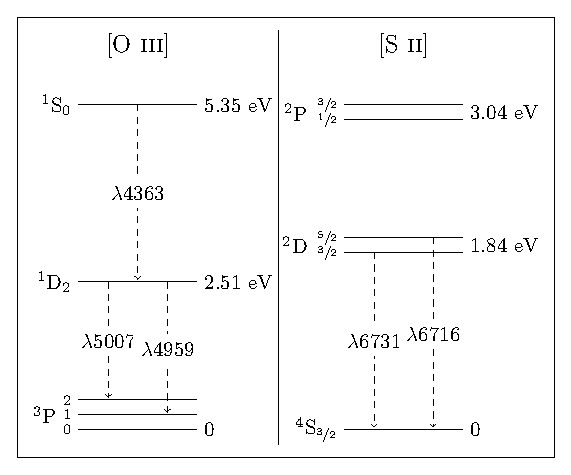
\includegraphics[width=0.5\textwidth]{Images/Paper1/energy_level_diagram-figure0}
	\caption[{[\ion{O}{3}] and [\ion{S}{2}] energy-level diagram}]{Energy-level 
	diagram for [O{\sc iii}] $(2p^2)$ and [S{\sc ii}] $(3p^3)$ ions.  The most 
	important transitions are shown; all are in the visible spectrum.  These 
	forbidden transitions in oxygen provide an estimate of the electron temperature 
	in the interstellar gas, while the forbidden sulfur transitions provide an 
	estimate of the electron number density.  With estimates of the electron 
	temperature and number density, we can convert emission line flux ratios into 
	chemical abundance ratios.}
	\label{fig:transitions_P1}
\end{figure}

% Gordon commented that this paragraph's phrasing needs to be modified if it is going into a paper, but it is fine for a thesis.  Is it too technical for a published paper?  What modifications might need to be made?
There are three significant emission lines for doubly-ionized oxygen.  The 
relative excitation rates to the $^1$S and $^1$D energy levels depend very 
strongly on the electron temperature, $T_e$; therefore, the relative strengths 
of these emitted lines can be used to measure the electron temperature 
\citep{Osterbrock89}.  In the low-density limit $(n_e < 10^5 \text{ cm}^{-3})$, 
most excitations to the $^1$D level result in an emission of a photon with a 
wavelength of either $5007\text{\AA}$ or $4959\text{\AA}$, as shown in Fig. 
\ref{fig:transitions_P1}.  Most excitations up to $^1$S produce a photon of 
wavelength $4363\text{\AA}$, followed by a photon of either of the two previous 
wavelengths (since the electron is now in the $^1$D level).

At higher densities, collisional de-excitation begins to influence these 
emission rates \citep{Osterbrock89}.  Because the $^1$D level has a longer 
lifetime than the $^1$S state, it is collisionally de-excited at lower electron 
densities.  This weakens the $\lambda 4959$ and $\lambda 5007$ emission lines.  
At the same time, the additional collisional excitations of the $^1$D state 
permitted by the higher electron densities strengthen the $\lambda 4363$ 
emission line.

[O{\sc iii}] $\lambda 4363$ is a temperature-sensitive forbidden transition line 
of doubly-ionized oxygen that is the preferred line to use when measuring the 
metallicity of galaxies.  Since the most effective cooling channel in these 
H{\sc ii} regions is oxygen line emission, lower metallicity regions have higher 
temperatures  \citep{Saintonge07}.  Collisional excitations up to this energy 
level are more common at higher temperatures, since there are more electrons 
with the kinetic energy required to excite the O$^{++}$ ion to this energy 
level.  As a result, the line strength of [O{\sc iii}] $\lambda 4363$ correlates 
with the region's temperature and is therefore anticorrelated with the 
metallicity of the galaxy.  [O{\sc iii}] $\lambda 4363$ is already one to two 
orders of magnitude weaker than the [O{\sc iii}] $\lambda \lambda 4959, 5007$ 
doublet, so it is very difficult to obtain an accurate ratio with this line.  It 
is for these reasons that other ``empirical'' relations were developed for 
metallicity calculations, eliminating the need for an electron temperature 
estimate from this emission line.

Given an electron temperature and density, the flux ratio of the [O{\sc iii}] 
$\lambda \lambda 4959, 5007$ doublet to H$\beta$ provides an abundance estimate 
for doubly-ionized oxygen.



%-------------------------------------------------------------------------------
\subsection{[\ion{O}{2}]}

A less temperature-sensitive line than [O{\sc iii}] $\lambda 4363$, the 
[O{\sc ii}] $\lambda 3727$ forbidden transition doublet of singly-ionized 
oxygen is often used in metallicity calculations.  With an electron temperature 
and density, its flux provides an estimate of the abundance of singly-ionized 
oxygen.  In SDSS spectra, this line can be observed for objects with a redshift 
greater than 0.02.  However, because dwarf galaxies are inherently faint objects 
($M_r > -17$), they are targeted for spectroscopy in SDSS only out to redshift 
$z\sim 0.03$, thus we can only estimate the metallicity of dwarf galaxies in the 
redshift range $0.02 < z < 0.03$.



%-------------------------------------------------------------------------------
% Sulfur
\subsection{[\ion{S}{2}]}

Just as we are able to measure the electron temperature from [O{\sc iii}] 
transitions, we can estimate the electron number density from [S{\sc ii}] 
transitions.  Below a density of about $100 \text{ cm}^{-3}$, the [S{\sc ii}] 
$\lambda 6716 / \lambda 6731$ ratio has a weak dependence on the density.  All 
our galaxies fall within this low-density regime, so we assume a low-density 
limit of $n_e = 100 \text{ cm}^{-3}$.

%Similar to the sensitivity of the doubly-ionized oxygen ion transitions to the 
%electron temperature of the surrounding gas, the transitions for singly-ionized 
%sulfur are sensitive to electron number density.  The relative excitation rates 
%depend only on the ratio of the collision strengths when two emission lines 
%(from the same ion) with nearly identical excitation energies are compared 
%\citep{Osterbrock89}.  If the two levels have different transition probabilities 
%and/or different collisional de-excitation rates, their ratio depends on the 
%density.
%
%The relative excitation rates of the two lines shown in Fig. 
%\ref{fig:transitions_P1} are proportional to their statistical weights; thus, the 
%ratio of the line intensities is a constant in the low-density limit 
%\citep{Osterbrock89}.  In the high-density regime, this ratio is best accurately 
%described by a Boltzmann population ratio.  There is a critical density for the 
%energy levels which describes the turning point between these two extremes.  


%-------------------------------------------------------------------------------
\subsection{Direct $T_e$ method}

We use the method published by \cite{Izotov06}, which is based on the 
astrophysics in \cite{Osterbrock89}.  It makes use of the [O{\sc iii}] 
$\lambda 4363$, $\lambda \lambda 4959, 5007$ lines and the [O{\sc ii}] 
$\lambda 3727$ doublet.  While often regarded as the most accurate estimate of 
the metallicity, it is difficult to employ due to the restrictions on 
[O{\sc iii}] $\lambda 4363$.  Consequently, this method is best suited for 
low-redshift, low-metallicity galaxies.  The electron temperature is derived by 
solving the following system of equations:
\begin{equation}
	t_3 = \frac{1.432}{\log[(\lambda 4959 + \lambda 5007)/\lambda 4363] - \log C_T}
\end{equation}
where $t_3 = 10^{-4} T_e(\text{O}^{++})$ and
\begin{equation}
	C_T = (8.44 - 1.09t_3 + 0.5t_3^2 - 0.08t_3^3)\frac{1 + 0.0004x_3}{1 + 0.044x_3}
\end{equation}
where $x_3 = 10^{-4} n_e t_3^{-0.5}$.  The ionic abundances are then found with 
the equations
\begin{align}
	12 + \log \left( \frac{\text{O}^+}{\text{H}^+} \right) &= \log \frac{\lambda 3727}{\text{H}\beta} + 5.961 + \frac{1.676}{t_2} - 0.40\log t_2 - 0.034t_2 + \log (1+1.35x_2) \\
	12 + \log \left( \frac{\text{O}^{++}}{\text{H}^+} \right) &= \log \frac{\lambda 4959 + \lambda 5007}{\text{H}\beta} + 6.200 + \frac{1.251}{t_3} - 0.55\log t_3 - 0.014t_3
\end{align}
where $t_2 = 10^{-4} T_e(\text{O}^+)$, $t_2 = 0.7t_3 + 0.3$ \citep{Garnett92}, 
and $x_2 = 10^{-4} n_e t_2^{-0.5}$.  \cite{Andrews13} show that this relation 
between $T_e(\text{O}^+)$ and $T_e(\text{O}^{++})$ may overestimate the 
temperature in the low ionization zone, causing the calculated metallicities to 
be underestimated.  Because we care only about the relative metallicity values 
of the galaxies, this effect will only affect our results in galaxies where 
O$^+$ dominates the oxygen abundance (where O$^+$/O$^{++} > 1$) in higher 
temperature regions (or low metallicities).  As shown in Fig. 
\ref{fig:O2O3_ratio}, this affects perhaps fifteen galaxies and does not change 
our conclusions.

\begin{figure}
    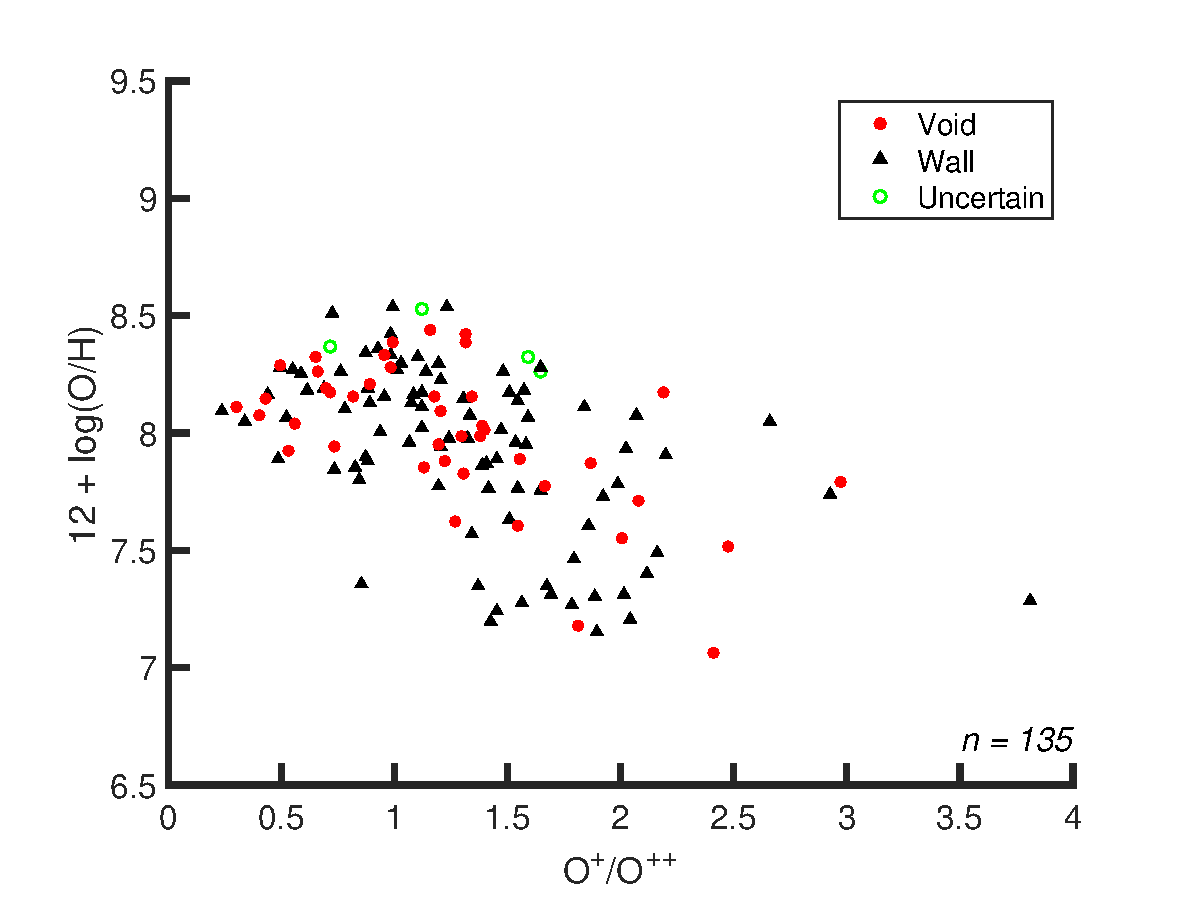
\includegraphics[width=0.5\textwidth]{Images/Paper1/1sig_I06_dwarf_SF_t3_OpOpp_Z12logOH}
    \caption[O$^+$/O$^{++}$ versus metallicity]{Metallicity of our 135 dwarf 
    galaxies as a function of O$^+$/O$^{++}$.  While either O$^+$ or O$^{++}$ 
    can dominate our galaxies' oxygen abundances, only those with low 
    metallicities (high temperatures) and with O$^+$ dominating the abundance 
    will be affected by the temperature overestimate of the low-ionization zone 
    as found by \cite{Andrews13}.  The small number of galaxies (15/135) that 
    may suffer from this possible temperature overestimate do not affect our 
    results.}
    \label{fig:O2O3_ratio}
\end{figure}  

The total gas-phase oxygen abundance is equal to the sum of the abundances of 
each of the ionized populations:
\begin{equation}
	\frac{\text{O}}{\text{H}} = \frac{\text{O}^{++}}{\text{H}^+} + \frac{\text{O}^+}{\text{H}^+}
\end{equation}



%%%%%%%%%%%%%%%%%%%%%%%%%%%%%%%%%%%%%%%%%%%%%%%%%%%%%%%%%%%%%%%%%%%%%%%%%%%%%%%%
%%%%%%%%%%%%%%%%%%%%%%%%%%%%%%%%%%%%%%%%%%%%%%%%%%%%%%%%%%%%%%%%%%%%%%%%%%%%%%%%
\section[Data]{SDSS data and galaxy selection}\label{sec:Data}
% What are the assumptions?
The SDSS Data Release 7 (DR7) \citep{Abazajian09} is a wide-field multi-band 
imaging and spectroscopic survey, using drift scanning to map approximately 
one-quarter of the northern sky.  Photometric data in the five band SDSS system 
--- $u$, $g$, $r$, $i$, and $z$ --- are taken with a dedicated 2.5-meter 
telescope at the Apache Point Observatory in New Mexico \citep{Fukugita96, 
Gunn98}.  Galaxies with a Petrosian $r$-band magnitude $m_r < 17.77$ are 
selected for spectroscopic analysis \citep{Lupton01, Strauss02}.  The spectra 
have an observed wavelength range of $3800\text{\AA}$ to $9200\text{\AA}$ with a 
resolution $\lambda / \Delta \lambda \sim 1800$, and are taken using two 
double fiber-fed spectrographs and fiber plug plates with a minimum fiber 
separation of 55 arcseconds \citep{Blanton03}.  The emission line flux data used 
in this study are from the MPA-JHU value-added catalog, which is based on the 
SDSS DR7 sample of galaxies.  Absolute magnitudes, colors, and all other 
additional data are from the KIAS value-added galaxy catalog \citep{Choi10}.


%-------------------------------------------------------------------------------
\subsection{Spectroscopic selection}

To satisfy the needs of our analysis, we make the following cuts to our sample.  
All analyzed galaxies must have relatively recent star formation, since UV 
photons are needed to excite the interstellar gas to produce the required 
emission lines.  As a result, each galaxy must have a star-forming BPT 
classification by \cite{Brinchmann04}.  In addition, because we analyze only 
dwarf galaxies ($M_r > -17$), there is a natural redshift upper limit of 0.03 on 
the samples; dwarf galaxies at higher redshifts are not bright enough to be 
included in the spectroscopic data of SDSS.  For a galaxy to be analyzed, we 
require a minimum $5\sigma$ detection of the H$\beta$ emission line and at least 
a $1\sigma$ detection of the [O{\sc iii}] $\lambda 4363$ forbidden transition.  
The restriction on both these lines eliminate those galaxies with a low S/N 
spectrum.  This is particularly important for [O{\sc iii}] $\lambda 4363$, as it 
is inherently a weak emission line.  We are aware that implementing this 
restriction on [O{\sc iii}] $\lambda 4363$ eliminates those galaxies with higher 
metallicities, since the strength of this line is inversely proportional to the 
metallicity of the galaxy (see Sec. \ref{sec:O3} for details).  However, we show 
that this restriction does not affect our conclusions on the large-scale 
environmental dependence on the gas-phase metallicity.

In addition, we also eliminate galaxies with temperature estimates 
$T_e (\text{O{\sc iii}}) > 3\times 10^4\text{ K}$.  Gas temperatures above this 
threshold are not physical for an H{\sc ii} region \citep[inferred 
from][]{Osterbrock89, Izotov06, Luridiana15}.

For the dwarf galaxies in our sample, the [O{\sc ii}] $\lambda 3727$ spectral 
line is very close to the edge of the spectrometer due to their maximum redshift 
$z < 0.03$.  Consequently, its flux measurement is not always reliable.  
Therefore, the flux values labeled \texttt{oii\_flux} in the MPA-JHU catalog are 
used instead of the combined flux values measured for the [O{\sc ii}] 
$\lambda \lambda 3726,3729$ doublet.  Because the velocity dispersion is not 
fixed when measuring the flux found in \texttt{oii\_flux}, the resulting 
measurements tend to be more realistic than those measured with the fixed 
dispersion (C. Tremonti, private communication).  In addition, those galaxies 
with remaining erroneous measurements for the [O{\sc ii}] $\lambda 3727$ 
doublet were removed by hand, after comparing the listed flux values to the 
spectra by eye.  All spectral lines used in the analysis must have a flux 
greater than 0, to ensure that they are emission lines.


%-------------------------------------------------------------------------------
\subsection{Void classification}

Void galaxies are identified using the void catalog compiled by \cite{Pan12}, 
which was built based on the galaxies in SDSS DR7 catalog.  Starting with 
galaxies with absolute magnitudes $M_r < -20$, the VoidFinder algorithm of 
\cite{Hoyle02} removes all isolated galaxies (defined as having the third 
nearest neighbor more than 7 $h^{-1}$ Mpc away).  After applying a grid to the 
remaining galaxies, spheres are grown from all empty grid cells (cells 
containing no galaxies).  A sphere reaches its maximum size when it encounters 
four galaxies on its surface.  To be classified as a void (or part of one), a 
sphere must have a minimum 10 Mpc radius.  If two spheres overlap by more than 
10\%, they are considered part of the same void.  See \cite{Hoyle02} for a more 
detailed description of the VoidFinder algorithm.  Those galaxies that fall 
within these void spheres are classified as void galaxies.  Those galaxies that 
lie outside the spheres are classified as wall galaxies.  Because we cannot 
identify any voids within 10 Mpc of the edge of the survey, we do not include 
the galaxies that fall within this region in either the void or wall sample 
(throughout this paper, these galaxies are labeled as ``Uncertain'').

Of the $\sim$ 800,000 galaxies with spectra available in SDSS DR7, 9519 are 
dwarf galaxies.  Applying the spectroscopic cuts, 42 void dwarf galaxies, 89 
wall dwarf galaxies, and 4 dwarf galaxies with uncertain large-scale 
environments are left to analyze (for a total of 135 dwarf galaxies, 131 of 
which are used in the environmental tests).


%%%%%%%%%%%%%%%%%%%%%%%%%%%%%%%%%%%%%%%%%%%%%%%%%%%%%%%%%%%%%%%%%%%%%%%%%%%%%%%%
%%%%%%%%%%%%%%%%%%%%%%%%%%%%%%%%%%%%%%%%%%%%%%%%%%%%%%%%%%%%%%%%%%%%%%%%%%%%%%%%
\section[Results]{Metallicity analysis and results}

Our primary objective is to perform a relative measurement of metallicity of 
dwarf galaxies to discern how the large-scale environment affects their chemical 
evolution.  As discussed in Section \ref{sec:Theory_P1}, the strength of and 
ability to observe different spectral lines between various surveys and 
observations require multiple methods to be developed for metallicity 
calculations.  In this paper, we use only the Direct $T_e$ method, because no 
other method has yet been calibrated using dwarf galaxies.  The results from the 
various methods are not directly comparable; while they all return metallicities 
within the same range, the same galaxy can have very different metallicity 
values depending on which method is used.  Conversions between methods have been 
developed \citep[see][]{Kewley08}, but it is not clear that these conversions 
would be accurate for dwarf galaxies.  Unfortunately, there are not enough 
galaxies available in our sample to calibrate these other methods for dwarf 
galaxies.  

All line ratios listed are ratios of the emission line fluxes.  Galaxies with 
low metallicities have $Z = 12 + \log (\text{O}/\text{H}) < 7.6$ 
\citep{Pustilnik06}; galaxies with high metallicities have $Z > 8.2$ 
\citep{Pilyugin06}.  The solar metallicity is $Z_{\odot} = 8.69\pm 0.05$ 
\citep{Asplund09}.


%-------------------------------------------------------------------------------
\subsection{Estimation of uncertainties and confirmation of our method}

% Uncertainties
We estimate uncertainties in the computed metallicity using a Monte-Carlo 
method.  Using the measured line fluxes and scaled uncertainty 
estimates\footnote{As described at 
\url{http://wwwmpa.mpa-garching.mpg.de/SDSS/DR7/raw_data.html}} from the 
MPA-JHU catalog, 100,000 different metallicities are calculated for a given 
galaxy.  For each estimate, the flux of a line is drawn from a normal 
distribution, with the expectation value being the original measured flux and 
the standard deviation being the given error in the flux measurement.  
We require all simulated line fluxes to be positive, as negative flux values 
would result in erroneous metallicity values.  The standard deviation in the set 
of these 100,000 calculated values is used as the error in the metallicity 
estimate for the galaxy.  As a result, these uncertainties tend to be larger 
than those quoted in other sources, as they include more information than just 
the quality of the fit used to derive the metallicity.

% Comparison to Yin07 metallicities for their galaxies
We compare results of our analysis of the same set of SDSS galaxies that 
\cite{Yin07} analyze to confirm that our code was working properly, since 
\cite{Yin07} also uses the metallicity method outlined in \cite{Izotov06}.  The 
results of this comparison can be seen in Fig. \ref{fig:Yin07_comp}.  
\cite{Yin07} also uses the MPA-JHU catalog as the source for their data, so our 
results should be identical.

\begin{figure}
    \centering
    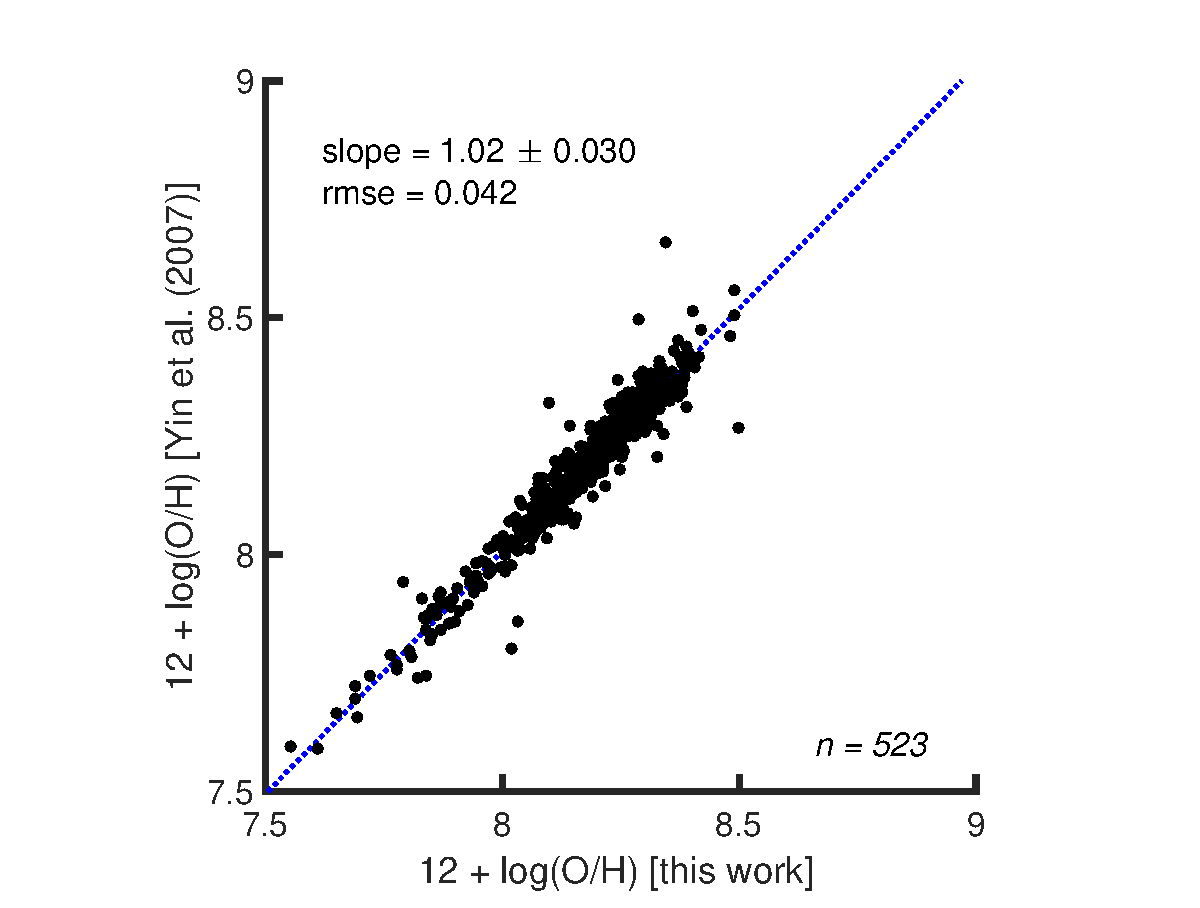
\includegraphics[width=0.5\textwidth]{Images/Paper1/Yin07_comparison_fit}
    \caption[Metallicity comparison to \cite{Yin07}]{Metallicity (\OH) 
    comparison between our calculated estimates and those made by \cite{Yin07}.  
    Error bars have been omitted for clarity.  These are not the dwarf galaxies 
    analyzed in this paper, but rather the sample of galaxies analyzed by 
    \cite{Yin07} to confirm that our version of the calculation is correct.  
    Both \cite{Yin07} and we have used the metallicity method outlined by 
    \cite{Izotov06}.}
    \label{fig:Yin07_comp}
\end{figure}


%-------------------------------------------------------------------------------
\subsection{Results}

\begin{figure*}
    \centering
    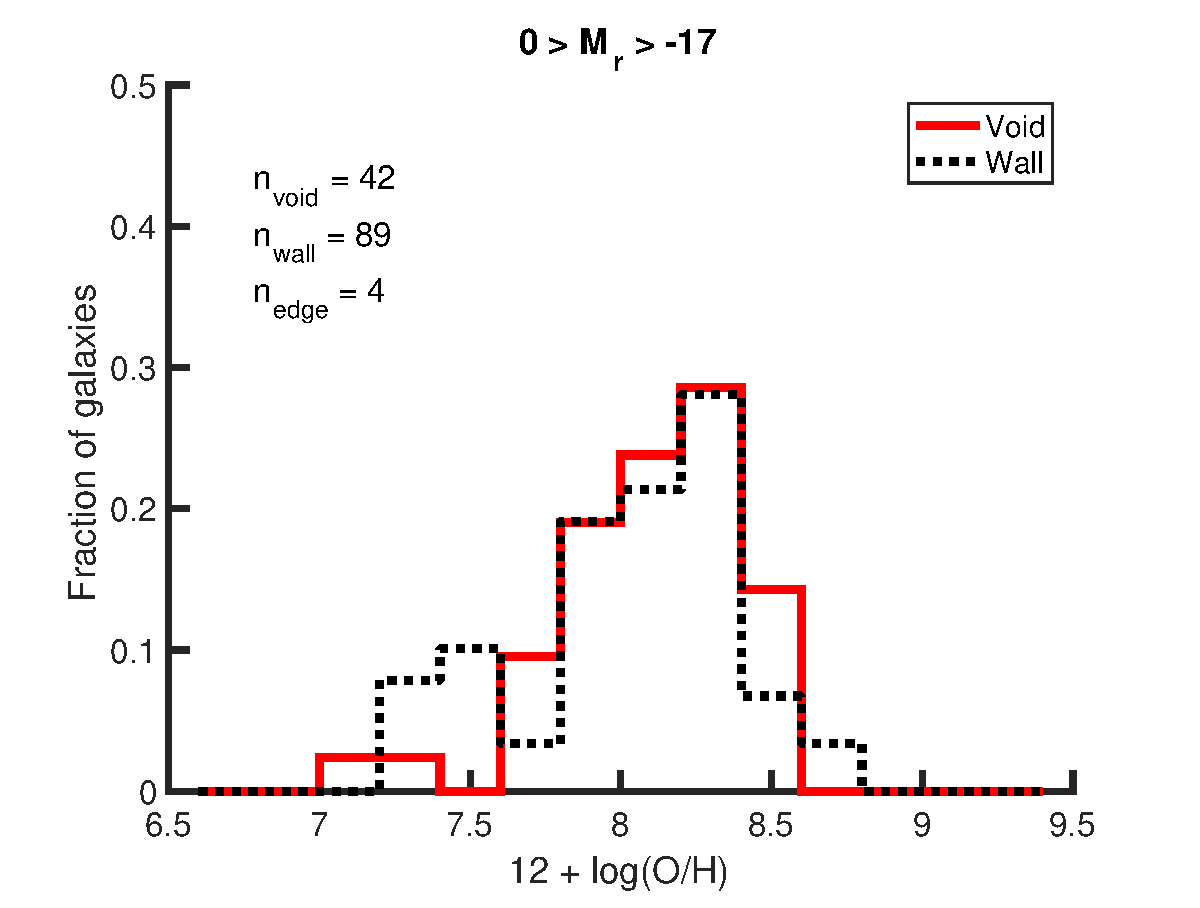
\includegraphics[width=0.49\textwidth]{Images/Paper1/1sig_dwarf_SF_t3_12logOH_hist}
    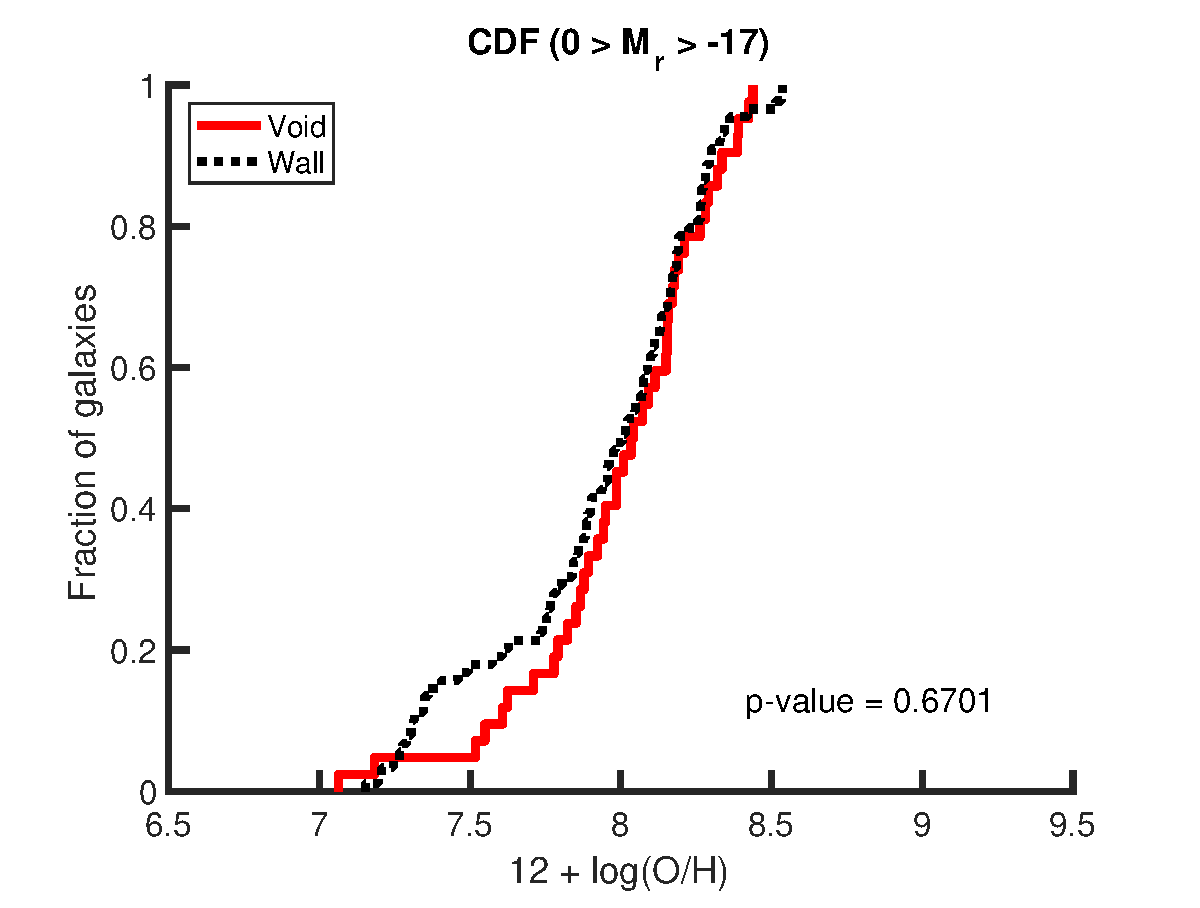
\includegraphics[width=0.49\textwidth]{Images/Paper1/1sig_dwarf_SF_t3_12logOH_CDF}
    \caption[Metallicity distribution of 135 dwarf galaxy sample]{Histogram and 
    associated cumulative distribution function of the gas-phase metallicity of 
    void dwarf (red solid line) and wall dwarf (black dashed line) galaxies.  A 
    two-sample KS test of the two data sets results in an asymptotic $p$-value 
    of 0.67, indicating a 67\% probability that a test statistic greater than 
    the observed value of 0.13 will be seen.  This is reflected visually, as 
    there appears to be very little difference in the two populations, 
    indicating that there is little large-scale environmental influence on the 
    metallicity of dwarf galaxies.}
    \label{fig:met1sig}
\end{figure*}

Metallicities calculated using the Direct $T_e$ method for our dwarf galaxy 
sample are listed in Table \ref{tab:Results_P1}, along with other key 
identification for the galaxies (including whether they are a void or wall 
galaxy).  A histogram of the resulting metallicities is shown in Fig. 
\ref{fig:met1sig}.  As can be seen in Fig. \ref{fig:met1sig}, there is very 
little difference in the spread of metallicity values in dwarf galaxies between 
voids and walls.  A two-sample Kolmogorov-Smimov (KS) test quantifies this 
observation --- it produced a test statistic of 0.13, corresponding to a 
probability of 67\% that a test statistic greater than or equal to that observed 
will be measured if the void sample were drawn from the wall sample; the 
cumulative distribution function (CDF) of these samples can be seen on the right 
in Fig. \ref{fig:met1sig}.

% Results table
\begin{sidewaystable}
\centering

\begin{tabular}{cccccccccccc}
Index\footnote{KIAS-VAGC galaxy index number} & R.A. & Decl. & Redshift & $M_r$ & \multicolumn{2}{c}{$12 + \log \left( \frac{\text{O}}{\text{H}} \right)$} & \multicolumn{2}{c}{$12 + \log \left( \frac{\text{N}}{\text{H}} \right)$} & \multicolumn{2}{c}{$\log \left( \frac{\text{N}}{\text{O}} \right)$} & Void/Wall \\
\hline \\
63713 & \RA{09}{20}{04}{.27} & -\dec{00}{30}{08}{.97} & 0.0257 & -16.73 & 7.80 & $\pm$0.41 & 6.83 & $\pm$0.28 & -0.97 & $\pm$0.49 & Wall \\
73537 & \RA{09}{25}{24}{.23} & +\dec{00}{12}{40}{.39} & 0.0250 & -16.94 & 7.94 & $\pm$0.34 & 6.76 & $\pm$0.24 & -1.18 & $\pm$0.41 & Wall \\
75442 & \RA{13}{13}{24}{.25} & +\dec{00}{15}{02}{.95} & 0.0264 & -16.81 & 7.55 & $\pm$0.35 & 6.73 & $\pm$0.24 & -0.82 & $\pm$0.42 & Void \\
168874 & \RA{11}{45}{13}{.16} & -\dec{01}{48}{17}{.68} & 0.0273 & -16.99 & 8.16 & $\pm$0.31 & 6.94 & $\pm$0.21 & -1.21 & $\pm$0.37 & Wall \\
184308 & \RA{09}{39}{09}{.38} & +\dec{00}{59}{04}{.15} & 0.0244 & -16.73 & 7.36 & $\pm$0.43 & 6.71 & $\pm$0.31 & -0.65 & $\pm$0.53 & Wall\\
\end{tabular}

\caption[Chemical abundances of subset of 135 dwarf galaxies]{Five of the 135 dwarf galaxies analyzed from SDSS DR7.  The flux values for all required emission lines can be found in the MPA-JHU value-added catalog.  Metallicity values are calculated using the direct $T_e$ method, with error estimates via a Monte Carlo method.  The void catalog of \cite{Pan12} is used to classify the galaxies as either Void or Wall.  If a galaxy is located too close to the boundary of the SDSS to identify whether or not it is inside a void, it is labeled as Uncertain.  (This table is available in its entirety in machine-readable form.)}

\label{tab:Results_P2}

\end{sidewaystable}


The requirement of a minimum $1\sigma$ detection of [O{\sc iii}] $\lambda 4363$ 
eliminates galaxies with a low-quality spectrum and those with a weak 
[O{\sc iii}] $\lambda 4363$ line.  Since this line is inversely proportional to 
the oxygen abundance in the interstellar gas, this biases the sample towards 
more low-metallicity galaxies.  To see how much this cut affects the results, we 
perform the same analysis with no minimum detection limit of [O{\sc iii}] 
$\lambda 4363$.  As can be seen in Fig. \ref{fig:met0sig}, this adds a 
substantial number of galaxies to the sample (there are now 126 void galaxies 
and 270 wall galaxies analyzed), predominately in the high-metallicity regime.  
As Table \ref{tab:Percents} makes apparent, there is now a higher percentage of 
void dwarf galaxies with high metallicities than wall dwarf galaxies.  However, 
the uncertainties in the metallicity estimates for 
$12 + \log (\text{O}/\text{H}) > 8.2$ are almost 0.5 dex, due to the extremely 
weak [O{\sc iii}] $\lambda 4363$ auroral line.  Because of these uncertainties, 
the difference in the distributions may not be statistically significant.

\begin{figure*}
    \centering
    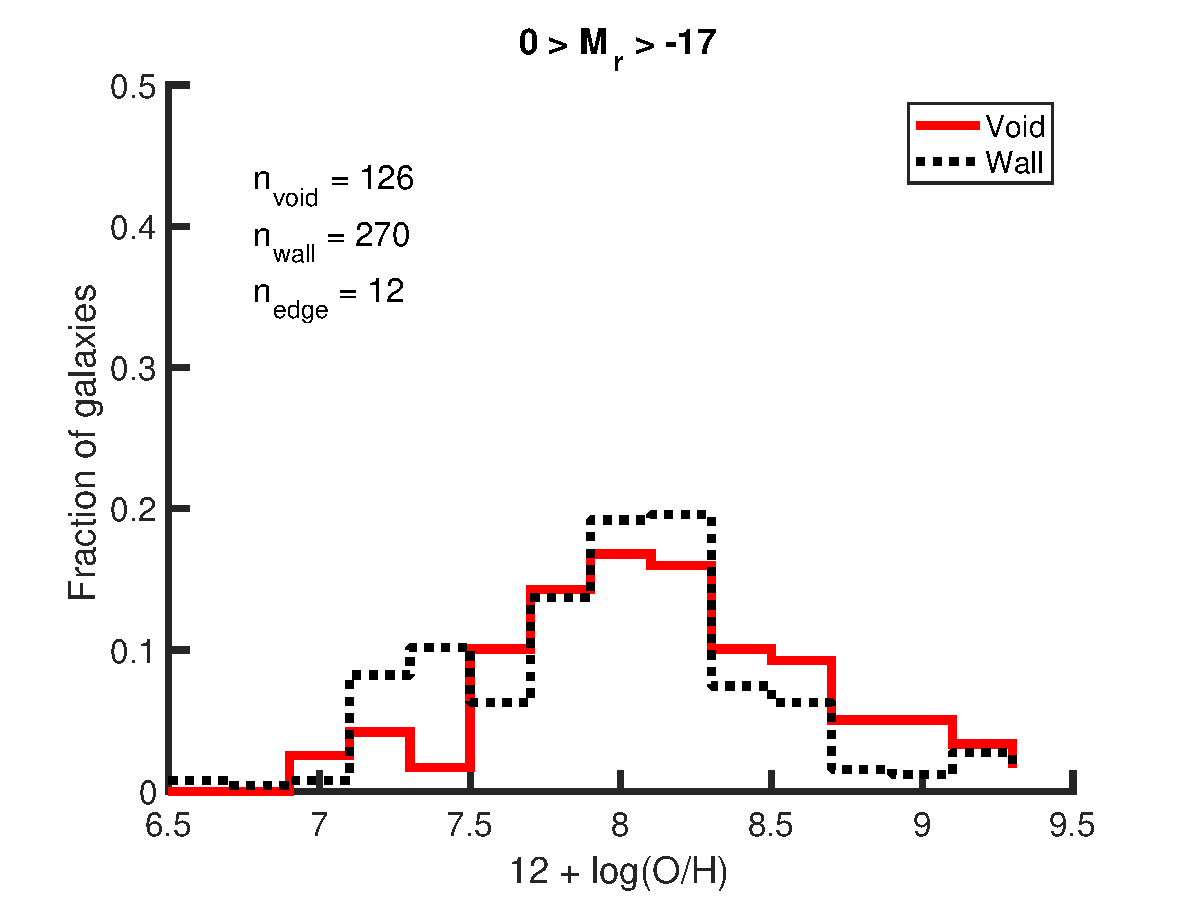
\includegraphics[width=0.49\textwidth]{Images/Paper1/0sig_dwarf_SF_t3_12logOH_hist}
    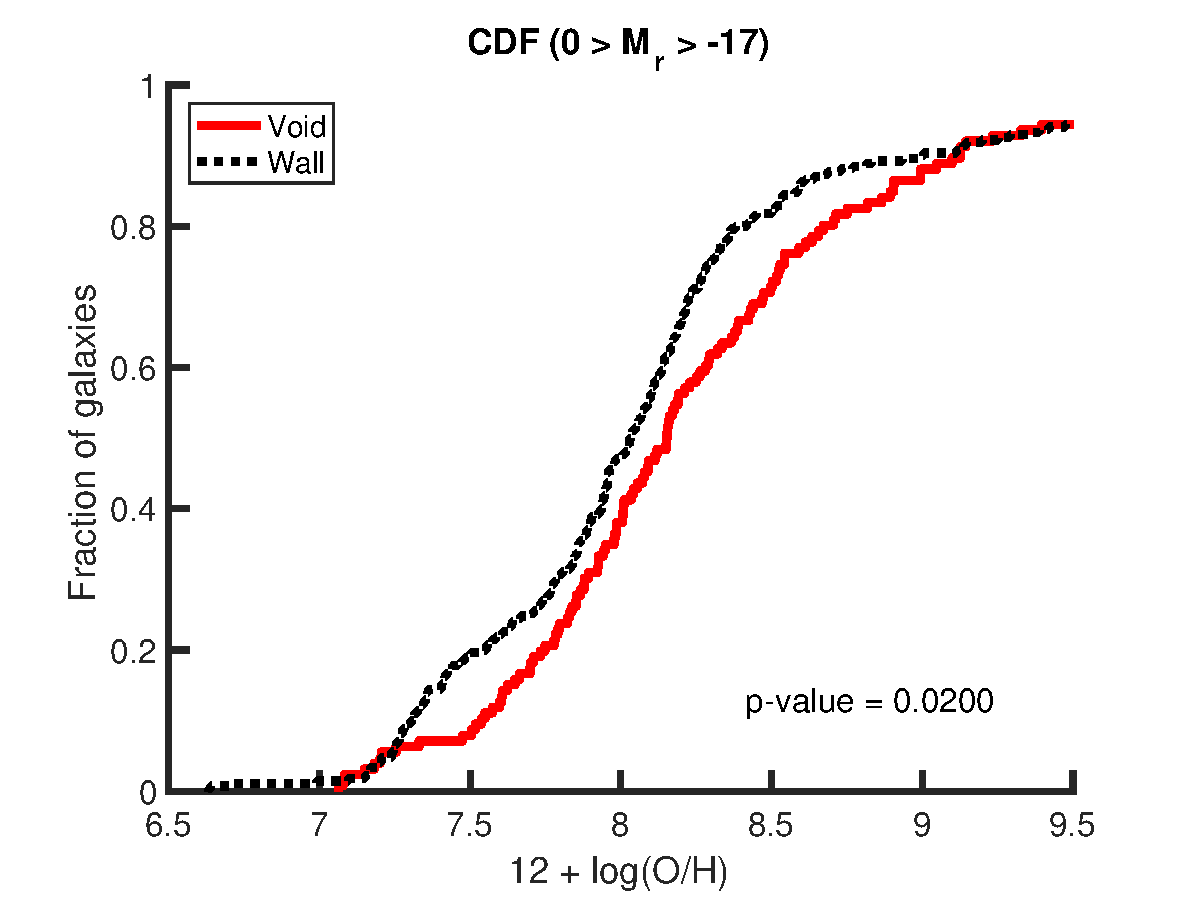
\includegraphics[width=0.49\textwidth]{Images/Paper1/0sig_dwarf_SF_t3_12logOH_CDF}
    \caption[{Metallicity distribution with no restriction on [\ion{O}{3}] 
    $\lambda 4363$}]{Histogram and associated cumulative distribution function 
    comparing the gas-phase metallicity of void dwarf (red solid line) and wall 
    dwarf (black dashed line) galaxies, testing the effect of the S/N 
    restriction on the auroral [O{\sc iii}] $\lambda 4363$ line.  The galaxies 
    here have no minimum detection of [O{\sc iii}] $\lambda 4363$ line.  As 
    expected, eliminating the restriction on this line includes more high 
    metallicity galaxies to the sample, shifting the void dwarf galaxy 
    distribution to have higher metallicities than the wall dwarf galaxies.  
    However, due to the significant uncertainties in the metallicity estimates 
    for $12 + \log (\text{O}/\text{H}) > 8.2$ due to the weak [O{\sc iii}] 
    $\lambda 4363$ auroral line, this difference in the distributions may not be 
    statistically significant.}
	\label{fig:met0sig}
\end{figure*}

\begin{table}
    \centering
    \begin{tabular}{cccc}
        \hline
         & $Z < 7.6$ & $7.6 \leq Z < 8.2$ & $Z \geq 8.2$\\
        \hline
        \hline
        \multicolumn{4}{c}{$1 \sigma$ restriction on [O{\sc iii}] $\lambda 4363$}\\
        \hline
        Void & 9.52\% (4)   & 66.67\% (28) & 23.81\% (10)\\
        Wall & 19.10\% (17) & 59.55\% (53) & 21.35\% (19)\\
        \hline
        \multicolumn{4}{c}{No restriction on [O{\sc iii}] $\lambda 4363$}\\
        \hline
        Void & 13.33\% (16) & 45.83\% (55)  & 40.83\% (49)\\
        Wall & 23.26\% (60) & 46.12\% (119) & 30.62\% (79)\\
        \hline
    \end{tabular}
    \caption[Metallicity distribution of 135 dwarf galaxy sample]{Percentages of 
    galaxies with calculated metallicities within the labeled metallicity 
    ranges, with the number of galaxies in each category in parentheses.  
    Removing the S/N restriction on [O{\sc iii}] $\lambda 4363$ especially 
    increases the number of dwarf galaxies with high metallicities, changing the 
    distribution so that void dwarf galaxies have higher metallicities than wall 
    dwarf galaxies.  However, due to the large uncertainties in the metallicity 
    estimates for $12 + \log (\text{O}/\text{H}) > 8.2$, this difference in the 
    distributions may not be statistically significant.\label{tab:Percents}}
\end{table}


%-------------------------------------------------------------------------------
\subsection{Sources of systematic error}

It is well-known that many physical properties of galaxies vary with the 
distance from the center of the galaxy \citep{Bell00}.  Therefore, a metallicity 
measurement is dependent on the location of the spectroscopic fiber on the 
galaxy.  If not all the light of the galaxy is contained within the fiber of the 
spectrograph, the estimated metallicity will not necessarily be representative 
of a global metallicity value.  Indeed, it has been shown that different parts 
of a galaxy have different metallicity values \citep{Bell00}.  In SDSS, the 
fiber size is 3 arcseconds -- this corresponds to a physical diameter between 
1.29 kpc and 1.93 kpc at redshifts $0.02 < z < 0.03$.  For many of the dwarf 
galaxies, this covers more than 50\% of the galaxy's luminous surface.  The 
fiber is almost always centered on the brightest spot of the galaxy.  For spiral 
and elliptical galaxies, this is often the center of the galaxy.  Since 
the metallicity of the center of a galaxy is often higher than at its edge, 
these metallicity values may be overestimates of the global metallicity.  Many 
dwarf galaxies are irregular galaxies, where the fiber is instead focused on a 
bright H{\sc ii} region.
% Consider rewording this part, to make it more concise and less wordy.

Due to the requirements we place on the emission lines for the galaxies, we are 
inherently limiting our sample to only blue, star-forming galaxies.  This is not 
a representative sample of the dwarf galaxy population.  Rather, in this study 
we are only able to comment on the large-scale environmental influence on blue, 
star-forming dwarf galaxies in a narrow redshift range.  Unfortunately, we 
cannot measure the metallicity of red dwarf galaxies with the Direct $T_e$ 
method, since we need the UV photons from young stars to excite the interstellar 
gas.

%Since SDSS is a magnitude-limited survey, there are many selection effects 
%inherent in the included galaxies.  Fortunately, since we are looking at only 
%dwarf galaxies with particular spectral lines, some of these selection effects 
%are eliminated, but includes others.  While these effects are expected to be 
%relatively minor, further study with other surveys will help determine if any of 
%these selection effects, especially aperture bias, have a significant influence 
%on our final results.


%-------------------------------------------------------------------------------
\subsection{Comparison to previously published metallicity measurements}

To place our metallicity measurements in the context of previous work, we 
compare our results to the metallicity values measured by \cite{Tremonti04}.  
While we both use data from the MPA-JHU value-added catalog, \cite{Tremonti04} 
employs an empirical method for estimating the metallicity, which is based on 
calibrated relationships between direct metallicity values and strong-line 
ratios.  The results of this comparison are shown in Figure \ref{fig:T04comp}.  
Unfortunately, the range of metallicity values found by \cite{Tremonti04} is 
limited to those galaxies with high metallicities 
$(12 + \log(\text{O}/\text{H}) > 8.5)$, due to the characteristics of their 
sample and their method; they found less than 2\% of their total sample to have 
metallicities less than 8.5.  \cite{Kennicutt03} shows that methods which make 
extensive use of the strong emission lines (so-called ``strong-line'' methods) 
can overestimate the metallicity abundances by as much as 0.3 dex.  A similar 
comparison is made in \cite{Yin07}, where they too find that the metallicity 
estimates of \cite{Tremonti04} are overestimated by 0.34 dex on average.  This 
can be seen quite clearly in Figure \ref{fig:T04comp}, as there is no 
correlation between galaxies with our estimates of 
$12 + \log (\text{O}/\text{H}) < 8$ and the metallicities measured by 
\cite{Tremonti04}, since their metallicities are much higher than ours.  The 
formal correlation coefficient between these two data sets is $0.00 \pm 0.087$; 
the correlation coefficient for those galaxies we measure to have metallicities 
greater than 7.6 (so excluding the low-metallicity galaxies) is 
$0.12 \pm 0.093$.  While this shows a slightly stronger correlation, we realize 
that these galaxies cover a limited range of metallicity values.  As a result, 
any scatter due to the errors in the calculations will result in a low 
correlation coefficient, which is what we see.  Therefore, by Fig. 
\ref{fig:T04comp}, we can see that there is a reasonable agreement between our 
metallicity values and those of \cite{Tremonti04}, excluding those galaxies we 
found to have extremely low metallicity values.

While it is known that there are systematic offsets between different 
metallicity calculation methods \citep{Kewley08}, that does not seem to be the 
case in the relation between our metallicities (measured with the Direct $T_e$ 
method) and those of \cite{Tremonti04} (measured with a combination of 
``strong-line'' methods).  While the metallicity estimates by \cite{Tremonti04} 
do not appear to be significantly biased at 
$8 < 12 + \log (\text{O}/\text{H}) < 8.5$, they overestimate the metallicities 
for low-metallicity galaxies.

\begin{figure}
    \centering
    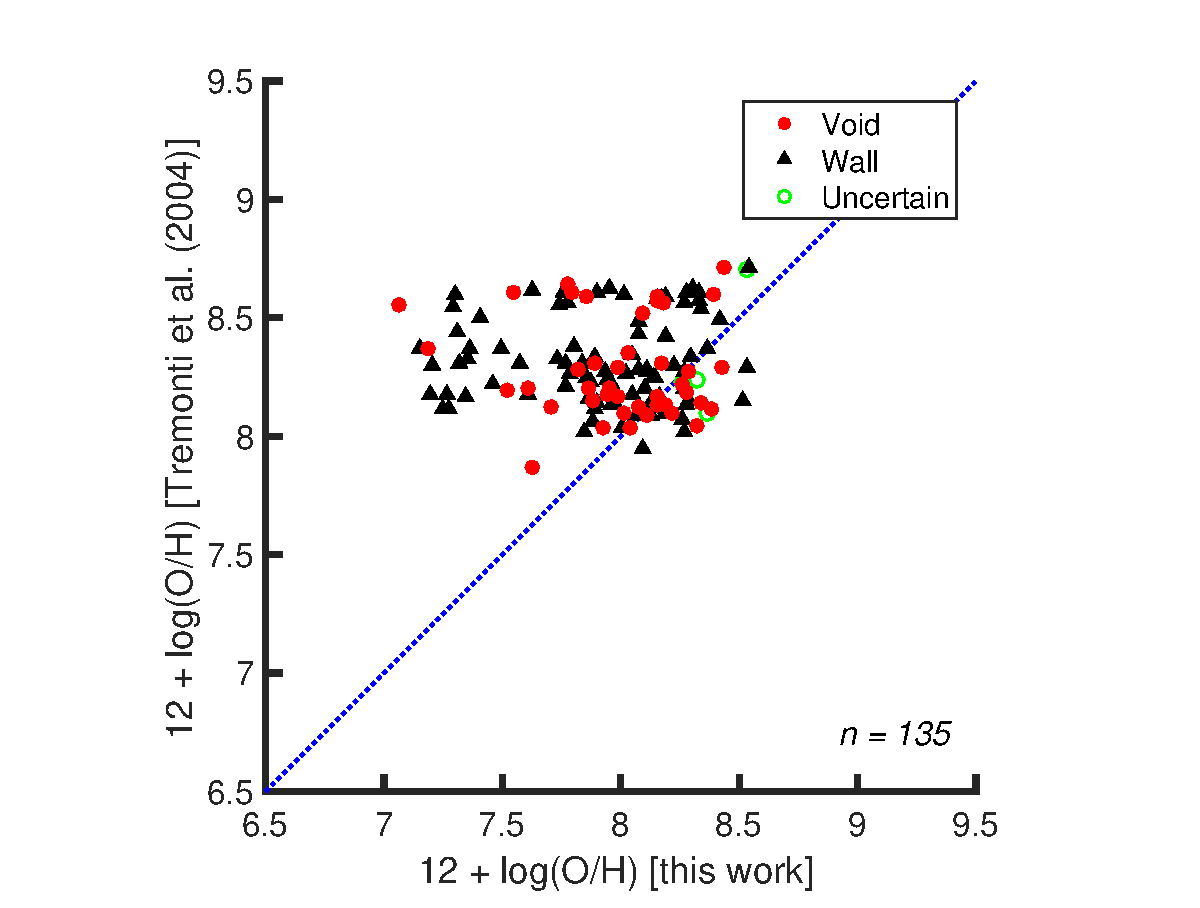
\includegraphics[width=0.5\textwidth]{Images/Paper1/1sig_dwarf_I06_SF_t3_T04comparison}
    \caption[Metallicity comparison to \cite{Tremonti04}]{Metallicity (\OH) 
    comparison between our calculated estimates and those made by 
    \cite{Tremonti04}.  Error bars have been omitted for clarity.  Excepting the 
    extreme low-metallicity galaxies we found, most galaxies agree reasonably 
    well with the values already published.  It is important to note that the 
    strong-line methods \citep[like those used by][]{Tremonti04} are not 
    calibrated for low-metallicity values and are known to overestimate the 
    metallicity by as much as 0.3 dex \citep{Kennicutt03}.  Thus, it is not 
    surprising that oxygen abundances measured using the direct method find 
    lower metallicity, particularly at very low metallicities.}
    \label{fig:T04comp}
\end{figure}

% None of the galaxies analyzed by Kreckel15 have SDSS spectra - they all have 
% magnitudes fainter than 17.77 (so they are too faint for the SDSS 
% spectrometer).

% None of the galaxies analyzed by Kniazev03 are in our sample - they are either 
% too close to measure [OII] 3727, or they are brighter than our absolute 
% magnitude limit.


%-------------------------------------------------------------------------------
\subsection{Mass-metallicity relation}

A strong correlation between the stellar mass and metallicity of galaxies 
reflects the fundamental connection between galactic mass and the chemical 
evolution of galaxies.  We use stellar mass estimates from the MPA-JHU catalog 
to examine the mass-metallicity relation in our sample of 135 dwarf galaxies.  
We have also included those galaxies from the MPA-JHU catalog with metallicity 
estimates from \cite{Tremonti04} to place our sample in context.  Due to the 
narrow range of masses in our sample, it is difficult to derive an accurate fit 
to the data.  However, we make comparisons to three published mass-metallicity 
relations \citep{Tremonti04, Mannucci10, Andrews13}.  As can be seen in Fig. 
\ref{fig:MZrelation}, the fit by \cite{Mannucci10} diverges at the low-mass 
limit, and the relations of \cite{Tremonti04} and \cite{Andrews13} predict 
metallicities that are higher than measured for most galaxies in this sample.  
It is important to note that two of these relations are only calibrated down to 
a stellar mass of $10^{8.5} M_{\odot}$.  In Fig. \ref{fig:MZrelation}, these 
relations have been extended to $10^{7.5} M_{\odot}$, in order to continue past 
our galaxy sample.

In addition to looking at the overall mass-metallicity relation for dwarf 
galaxies, we can also investigate the difference in the relation between 
galaxies in voids and those in more dense regions.  There appear to be no 
significant differences in the two populations, indicating minimal influence 
from the large-scale environment on the mass-metallicity relation of these dwarf 
galaxies.  \cite{Hughes13} also find that the stellar mass-metallicity relation 
is independent of large-scale environment.  This prompts the conclusion that the 
internal evolutionary processes of a galaxy have a greater influence on its 
chemical evolution than its large-scale environment.  We expect this dependence 
of the chemical content of a galaxy on its stellar mass, since the accumulated 
metals reflect the integrated history of star formation.  However, we would 
expect an environmental dependence to appear as well, if void galaxies are in an 
earlier stage of evolution and/or are continuing to accrete fresh gas.

\begin{figure}
    \centering
    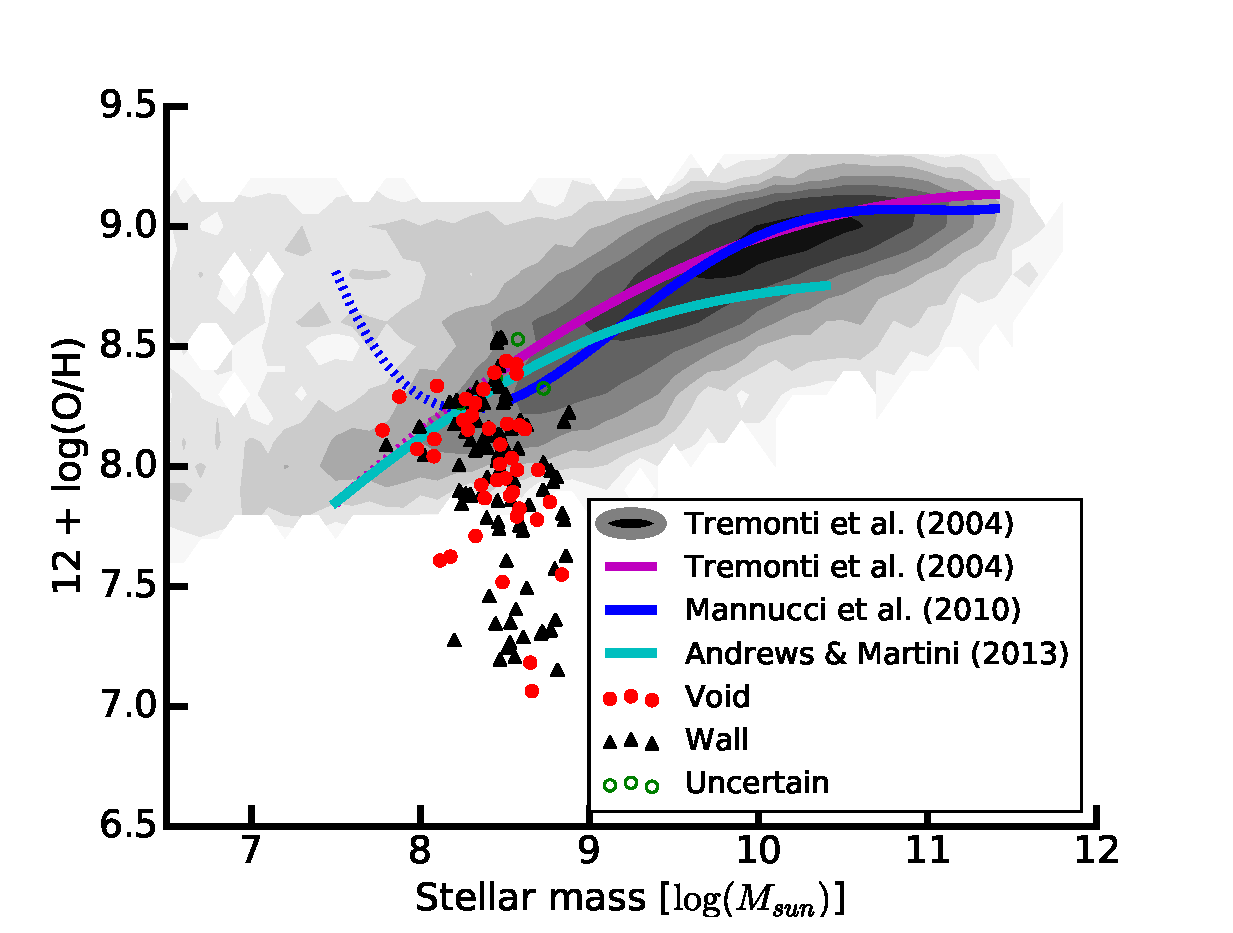
\includegraphics[width=0.5\textwidth]{Images/Paper1/MZ_1sig_I06_dwarf_SF_t3_python}
    \caption[Stellar mass versus metallicity for 135 dwarf galaxy sample]
    {Stellar mass versus metallicity of the 135 analyzed dwarf galaxies.  Error 
    bars have been omitted for clarity.  Due to the limited range of mass (all 
    our galaxies are within a small range of masses, since we are looking only 
    at dwarf galaxies), we cannot derive our own relation between the mass and 
    metallicity.  Some previously published relations are plotted over our data 
    for comparison.  To place our sample in context, we have also included (grey 
    contours) those galaxies from the MPA-JHU catalog with metallicity estimates 
    by \cite{Tremonti04}.  It was from these galaxies that the published 
    relation of \cite{Tremonti04} was derived.}
    \label{fig:MZrelation}
\end{figure}



%-------------------------------------------------------------------------------
\subsection{SFR-metallicity relation}

A fundamental diagnostic of the star formation history of galaxies is the 
relation between stellar mass, metallicity, and star formation rate.  Therefore, 
we also look at the relationship between the (specific) star formation rate and 
metallicity of these 135 dwarf galaxies.  The total (specific) star formation 
rate estimates for these galaxies are from the MPA-JHU value-added catalog, 
based on the technique discussed in \cite{Brinchmann04}.  For low-mass galaxies, 
\cite{Henry13} show that the metallicity is inversely proportional to the star 
formation rate of a galaxy.  However, this is not what is observed in our data, 
as seen in Fig. \ref{fig:SFRZ_relation}.  The correlation coefficient between 
the total (specific) star formation rate and the metallicity 
$r_{sSFR} = 0.49 \pm 0.066$ and $r_{SFR} = 0.52 \pm 0.063$, showing a positive 
correlation between the two properties.  Indeed, those galaxies with the lowest 
metallicities have some of the lowest (specific) star formation rates among the 
dwarf galaxies in our sample.  Since we are limiting our sample to only 
star-forming galaxies, the (s)SFR must be relatively high to emit the UV photons 
needed to ionize the gas.  As a result, all low (s)SFR galaxies will be 
eliminated from our sample, as seen in Fig. \ref{fig:SFR_distribution}.  In 
addition, due to the behavior of the [O{\sc iii}] $\lambda 4363$ auroral line, 
all galaxies with metallicities $12 + \log (\text{O}/\text{H}) \gtrsim 8.5$ are 
also eliminated from the sample.  As a result, we are only calculating the 
metallicity of galaxies in the lower right corners of the (s)SFR plots in Fig. 
\ref{fig:SFRZ_relation}, which is why we see the unexpected correlation.  There 
does not seem to be a difference between the void and wall galaxies in this 
relation, indicating no large-scale environmental influence on the (s)SFR--Z 
relation.

\begin{figure*}
    \centering
    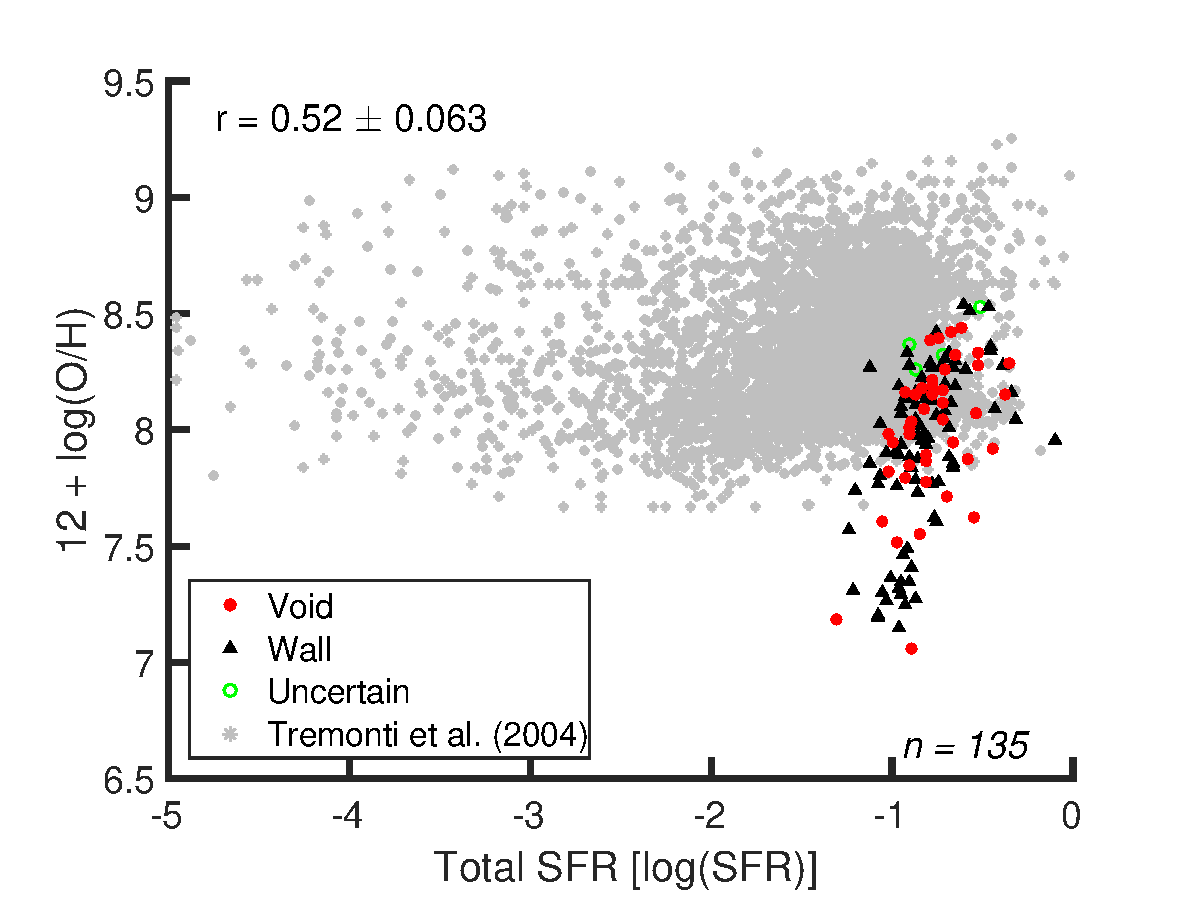
\includegraphics[width=0.49\textwidth]{Images/Paper1/SFR_OH_1sig_I06_dwarf_SF_t3}
    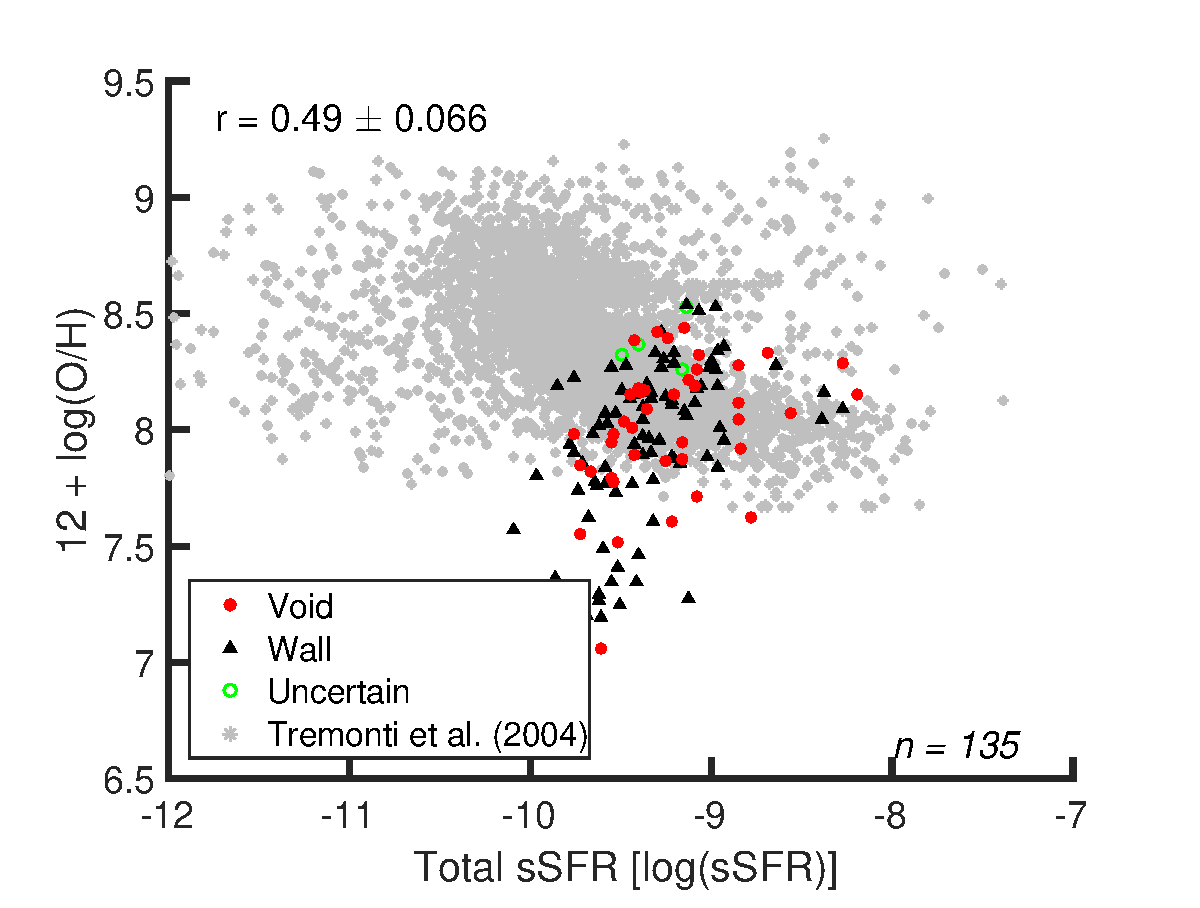
\includegraphics[width=0.49\textwidth]{Images/Paper1/sSFR_OH_1sig_I06_dwarf_SF_t3}
    \caption[(s)SFR versus metallicity for 135 dwarf galaxy sample]{Total star 
    formation rate (SFR) and specific star formation rate (sSFR) versus 
    metallicity of the 135 analyzed dwarf galaxies.  Error bars have been 
    omitted for clarity.  We also plot (grey stars) dwarf galaxies ($M_r > -17$) 
    with metallicity estimates by \cite{Tremonti04}, to place our results in 
    context.  It is significant to note that the majority of our galaxies are on 
    the upper end of the SFR and sSFR for dwarf galaxies, as shown in Fig. 
    \ref{fig:SFR_distribution}.  Note that those galaxies with metallicities 
    $12 + \log(\text{O}/\text{H}) < 7.6$ are on the lower end of the range of 
    sSFR of the dwarf galaxies in our sample.}
    \label{fig:SFRZ_relation}
\end{figure*}

\begin{figure*}
    \centering
    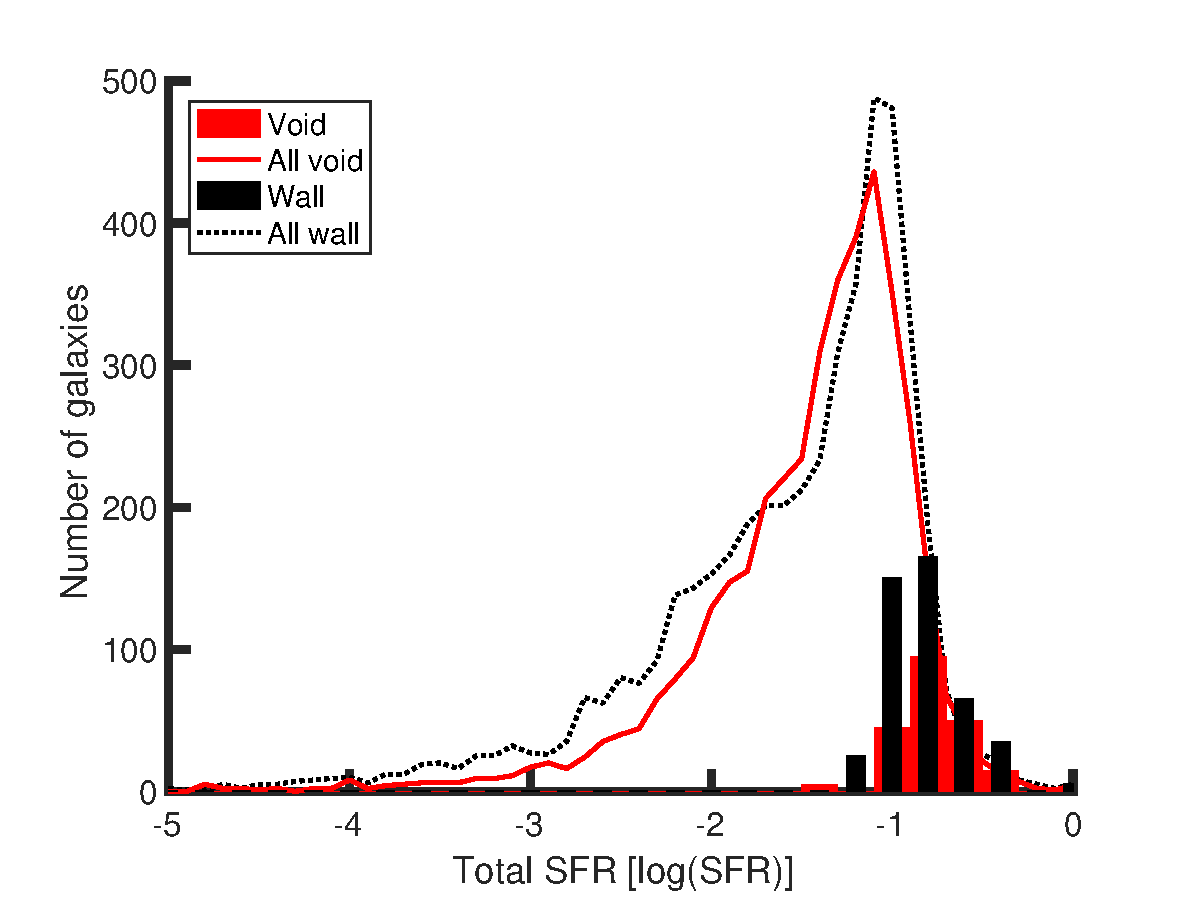
\includegraphics[width=0.49\textwidth]{Images/Paper1/1sig_I06_SF_t3_SFR_scaled}
    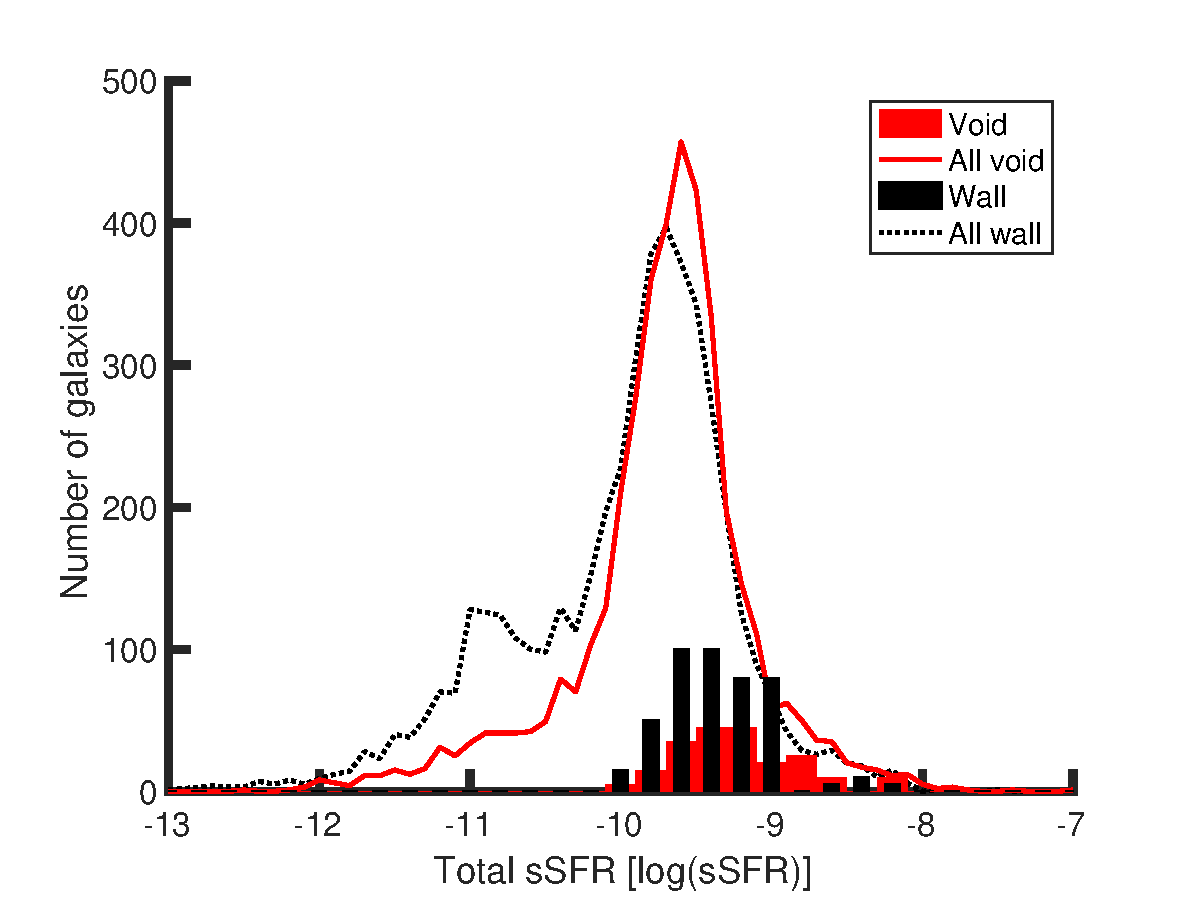
\includegraphics[width=0.49\textwidth]{Images/Paper1/1sig_I06_SF_t3_sSFR_scaled}
    \caption[Distribution of (s)SFR for 135 dwarf galaxy sample compared to SDSS]
    {Distribution of the total star formation rate (SFR) and specific star 
    formation rate (sSFR) for void and wall dwarf galaxies in SDSS are shown in 
    the red solid and black dashed lines, respectively.  Our sample of dwarf 
    galaxies (with metallicity values) is shown in the red and black bars 
    (scaled by a factor of 5 for greater visibility).  We are looking only at 
    the highest SFR found in dwarf galaxies; the sSFR for our sample of dwarf 
    galaxies follows the distribution of all dwarf galaxies.  There is clearly a 
    selection bias against lower SFR.}
    \label{fig:SFR_distribution}
\end{figure*}



%-------------------------------------------------------------------------------
\subsection{Color-metallicity relation}

Metallicity is expected to have a positive correlation with color, as older 
galaxies are expected to have higher metallicities, since they have had more 
time to convert their gas into heavier elements through star formation.  
Therefore, we also look at the color--metallicity relation of our sample of 
135 galaxies -- these relations can be seen in Fig. \ref{fig:colorZ_relation}.  
To place our galaxies in the context of other dwarf galaxies, we have included 
the sample of dwarf galaxies for which \cite{Tremonti04} has estimated 
metallicities (grey stars in the figures).

As we can see in Fig. \ref{fig:colorHist}, by overlaying our distribution of 
dwarf galaxies on Fig. 4 of \cite{Hoyle12}, all of our dwarf galaxies are 
members of the blue dwarf galaxy population.  (The Gaussian parameters for the 
curves are taken from Table 3 in \cite{Hoyle12}.)  This is as expected, since 
the Direct $T_e$ method requires measurements of the emission lines of the 
galaxies; these emission lines are caused by the UV photons of newly formed 
stars, indicating a star-forming galaxy and giving the galaxy a blue color.

While the majority of our galaxies follow the positive correlation between color 
and metallicity, the group of extremely low-metallicity galaxies is less blue 
than their metallicities would indicate.  However, when compared to the red/blue 
curves in Fig. \ref{fig:colorHist}, these galaxies occupy the typical range of 
blue dwarf galaxies, so their colors are not unique.  There is no clear 
separation between the void and wall dwarf galaxies in Fig. 
\ref{fig:colorZ_relation}, indicating that there is little or no large-scale 
environmental influence on the color-metallicity relation of these galaxies.

\begin{figure*}
    \centering
    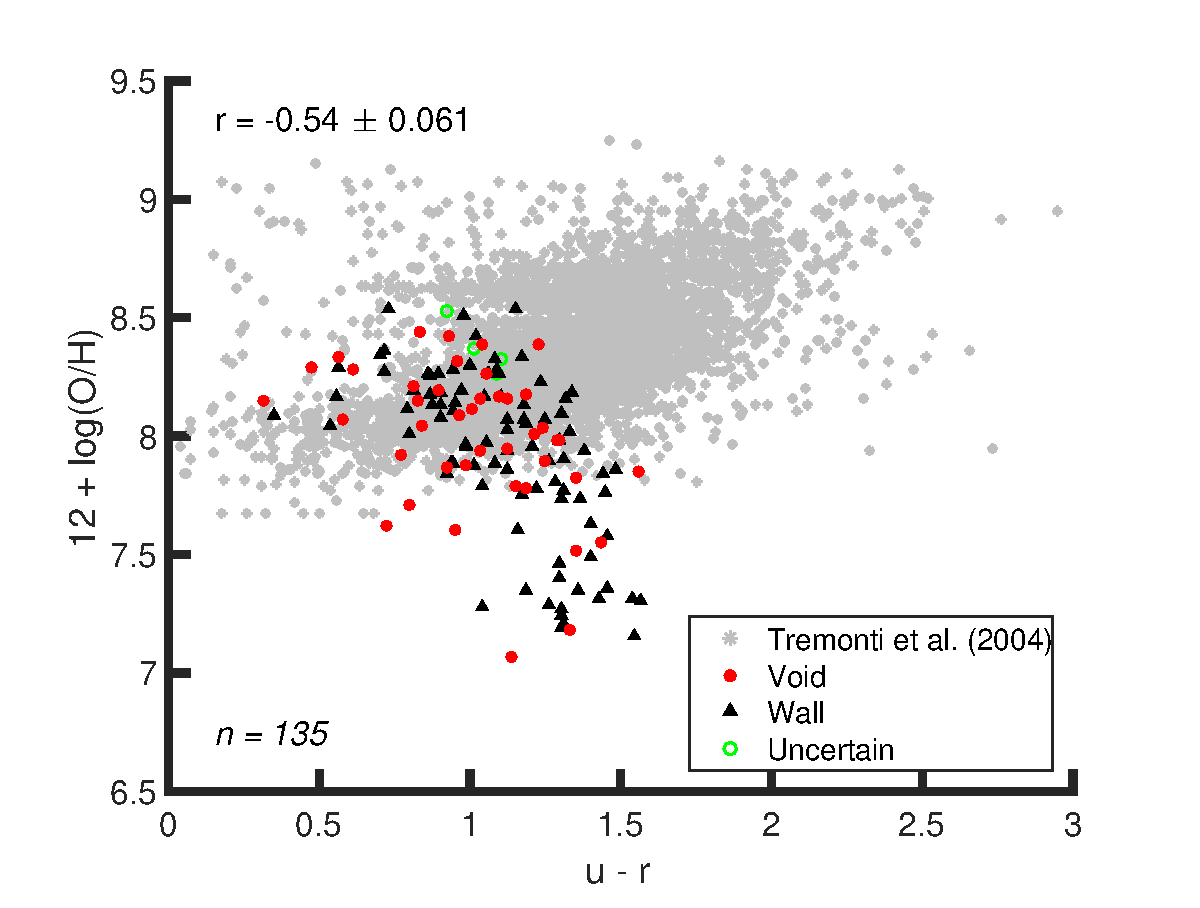
\includegraphics[width=0.49\textwidth]{Images/Paper1/ur_OH_1sig_I06_dwarf_SF_t3}
    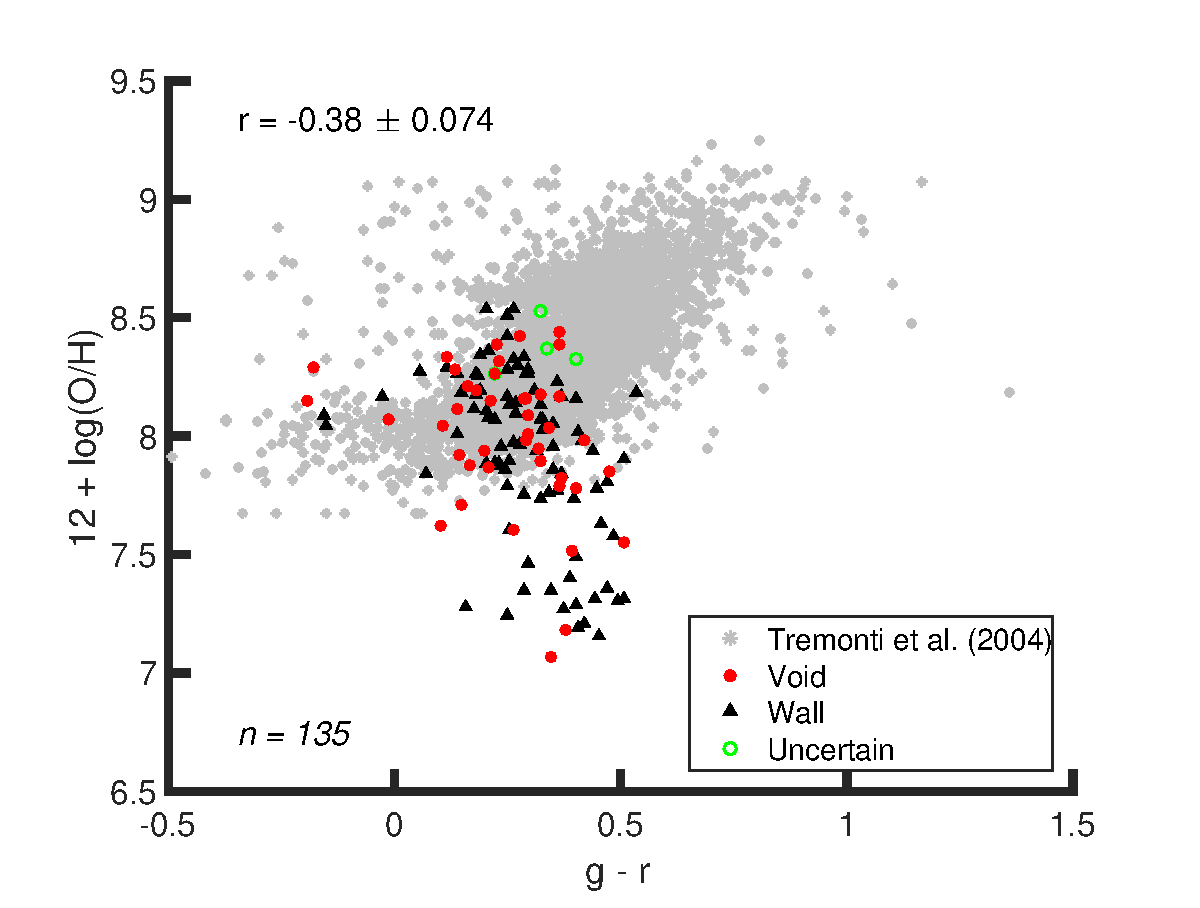
\includegraphics[width=0.49\textwidth]{Images/Paper1/gr_OH_1sig_I06_dwarf_SF_t3}
    \caption[Color versus metallicity for 135 dwarf galaxy sample]{Color (u--r 
    and g--r) versus metallicity of the 135 analyzed dwarf galaxies.  Error bars 
    have been omitted for clarity.  Metallicity is expected to have a positive 
    correlation with color, as older galaxies are expected to have higher 
    metallicities.  To place our galaxies in the context of the dwarf galaxy 
    population, we also plot (grey stars) dwarf galaxies ($M_r > -17$) with 
    metallicity estimates by \cite{Tremonti04}.  We find no significant 
    difference between the void and wall dwarf galaxies, indicating little to no 
    large-scale environmental influence on the color-metallicity relation.}
    \label{fig:colorZ_relation}
\end{figure*}

\begin{figure}
    \centering
    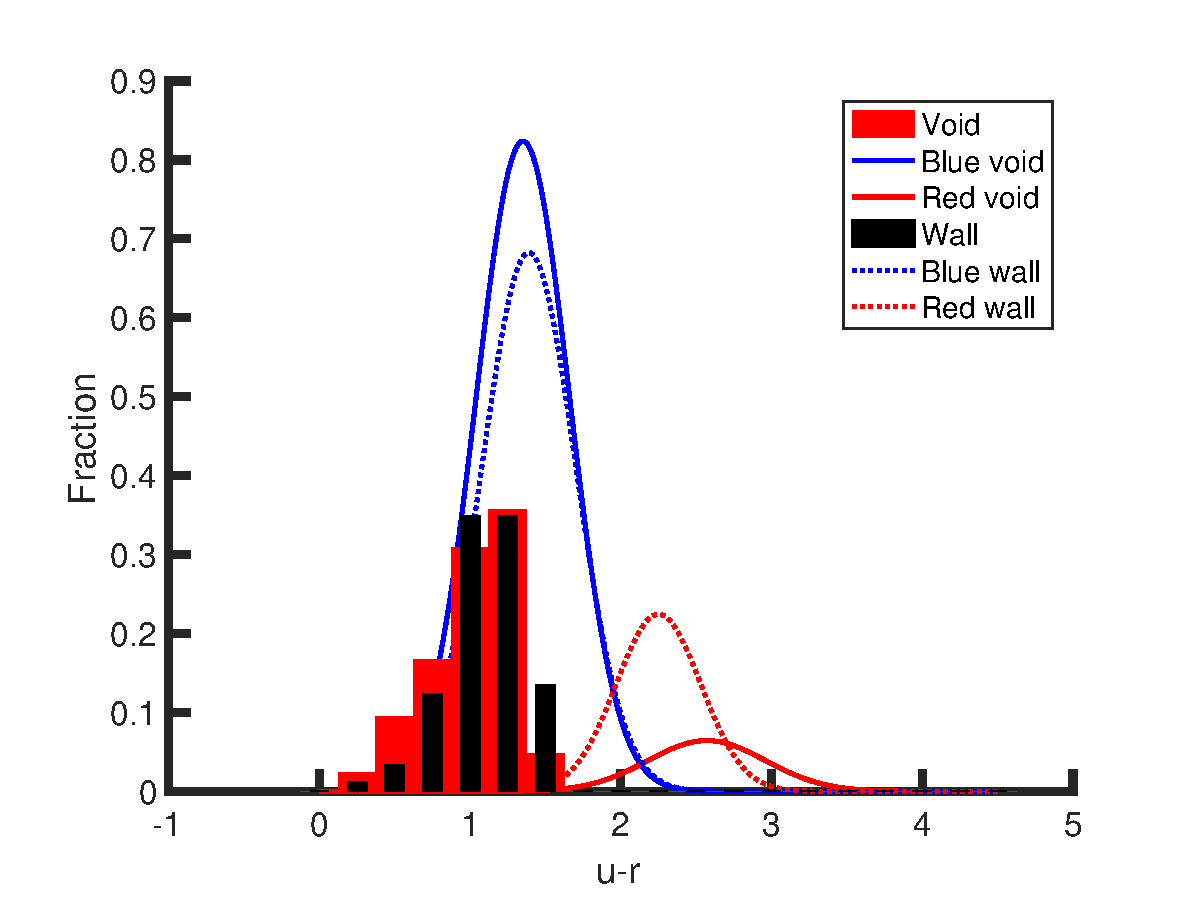
\includegraphics[width=0.5\textwidth]{Images/Paper1/urHist_1sig_I06_dwarf_SF_t3}
    \caption[Color distribution of 135 dwarf galaxy sample compared to SDSS]{The 
    $u-r$ color distribution of our 135 dwarf galaxies (red/black histograms) as 
    compared to the color distribution of all SDSS dwarf galaxies as found in 
    Fig. 4 of \cite{Hoyle12} (red/blue curves).  It is clear that our galaxies 
    are among the bluest dwarf galaxies in SDSS.}
    \label{fig:colorHist}
\end{figure}



%%%%%%%%%%%%%%%%%%%%%%%%%%%%%%%%%%%%%%%%%%%%%%%%%%%%%%%%%%%%%%%%%%%%%%%%%%%%%%%%
%%%%%%%%%%%%%%%%%%%%%%%%%%%%%%%%%%%%%%%%%%%%%%%%%%%%%%%%%%%%%%%%%%%%%%%%%%%%%%%%
\section{Discussion}
% Is there any point in actually running these calculations?

%-------------------------------------------------------------------------------
\subsection{Comparison to literature results}

We find no clear distinction between the metallicities of dwarf galaxies in 
voids and dwarf galaxies in more dense regions.  This result agrees with the 
results of \citet{Mouhcine07, Cooper08, Nicholls14a, Kreckel15} but disproves 
our initial hypothesis and contradicts the published results of 
\cite{Pustilnik06, Pustilnik11a, Pustilnik14, SanchezAlmeida16}.  
\cite{Cooper08} concludes that metal-rich galaxies preferentially reside in 
high-density regions.  Due to our requirement on the [O{\sc iii}] $\lambda 4363$ 
auroral line, we have very few dwarf galaxies with high metallicities.  As a 
result, we are not able to confirm their conclusions. \cite{Deng11} also reports 
a relationship between environment and metallicity.  However, he highlights a 
large difference in metallicity as a function of redshift which correlates with 
his two samples.  It is possible that the dependence he found is actually the 
result of a systematic dependence on redshift in their metallicity calculation.

Many studies suggest that the metallicity of void galaxies should, on average, 
be lower than that of galaxies in more dense regions.  \cite{Mouhcine07} and 
\cite{Cooper08} both perform statistical studies of this relationship on SDSS 
DR4, and \cite{Deng11} repeats this with the DR7 data (only looking at galaxies 
with a redshift $z > 0.02$).  \cite{Mouhcine07} conclude that the relation 
between stellar mass and metallicity is much stronger than that between a 
galaxy's environment and its metallicity.  \cite{Cooper08} find a more 
substantial correlation between a galaxy's environment and its metallicity, but 
point out that the noise of the different methods used to calculate metallicity 
is larger than any environment-metallicity relation.  Our analysis shows that 
there is very little difference between void and wall dwarf galaxies, suggesting 
that the large-scale environment does not strongly influence a dwarf galaxy's 
chemical evolution.

%-------------------------------------------------------------------------------
\subsection{Large-scale environmental influence}
% What does this mean?

% Description of void galaxies (theory)
Consideration of interactions between the interstellar medium (ISM), 
circumgalactic medium (CGM), and intergalactic medium (IGM) suggests that void 
galaxies should have relatively lower metallicity than galaxies in denser 
environments.  We find no such trend, perhaps because the IGM around 
star-forming ``wall galaxies'' in our sample is similar to that of void 
galaxies.

Simulations by \cite{Cen11} show that the entropy of gas in the IGM in voids 
remains below the critical entropy (defined to be when the cooling time of the 
gas is equal to the Hubble time), so the gas from the IGM can cool and fall into 
a void galaxy's CGM.  In a galaxy's ISM, supernovae expel gas (primarily 
metal-rich) into the CGM.  This gas has a higher metallicity than the average 
metallicity of the ISM \citep[shown by][]{Muratov17}.  While some of this gas 
reaches the outer edge of the CGM, most of it cools and falls back onto the 
galaxy's ISM, after having mixed with the hydrogen that has entered the CGM from 
the IGM.  Therefore, the gas falling back into the galaxy's ISM has a lower 
metallicity than the galaxy's ISM.

% Description of wall galaxies (theory)
In contrast to the void galaxies, the IGM around most wall galaxies is not cool 
enough to fall back onto the CGM.  \cite{Cen11} shows that, in general, the IGM 
of a wall galaxy has an entropy higher than the threshold for cooling.  As a 
result, most of the gas that falls back onto a wall galaxy's ISM is not as 
diluted as what falls onto a void galaxy's ISM.  This is where our hypothesis 
originated: because wall galaxies no longer have a source of cool hydrogen in 
the IGM, their metallicities will be higher than that of the void galaxies (for 
a fixed stellar mass).

% What do we actually see, and why?
However, Fig. \ref{fig:met1sig} does not reveal a lower metallicity in void 
galaxies.  Instead, our results indicate that there is no difference in the 
distribution of metallicities in wall and void galaxies.  In detail, Fig. 10 of 
\cite{Cen11} shows that not all wall galaxies rise above the entropy threshold.  
This is also coincident with the sSFR of the galaxies --- those galaxies with 
higher sSFRs are below the entropy threshold, while those with low sSFRs are 
above (independent of their large-scale environment).  Since all our galaxies 
have relatively high sSFRs (as required by the analysis --- star formation is 
required to detect the emission lines necessary for the metallicity 
calculations), it is possible that our population of wall dwarf galaxies is 
still surrounded by a cool IGM, similar to that of the void galaxies.  As a 
result, the wall galaxies still have a source of cool hydrogen, so the resulting 
distribution of the metallicities in the wall and void dwarf galaxies is the 
same.  \cite{Brisbin12} show that most star-forming galaxies with 
$M_* < 2.0\times 10^{10} M_{\odot}$ appear to be fed by the infall of pristine 
or low-metallicity gas.  \cite{Moran12} also find that the lowest-mass galaxies 
($\log(M_*) < 10.2 M_{\odot}$) have a sharp decline in their metallicity at 
large radii; coupled with a strong correlation to the galaxies' H{\sc i} masses, 
they concluded that this indicates newly accreted pristine gas in the galaxies.  
It appears that the large-scale (10 $h^{-1}$ Mpc) has little effect on the 
chemical evolution of galaxies; a galaxy's medium-scale (2 $h^{-1}$ Mpc) 
environment might have much more influence on its chemical evolution.

%There are a few possible explanations as to why there is no difference in the 
%metallicity of void and wall dwarf galaxies.  The recycling of the interstellar 
%medium (ISM) of a galaxy can be described by models that lie at two extremes: a 
%``closed box'' and an ``open box'' model.  In its simplest form, the closed box 
%model \citep{Talbot71} describes a galaxy that has no interaction with its 
%environment --- no material enters or leaves the region.  A galactic fountain 
%\citep{Shapiro76} is a good visualization of the closed box model --- any gas 
%expelled during a supernova falls back onto the galaxy.  In this model, the gas 
%is very turbulent and thus stays well-mixed throughout the galaxy.  Due to the 
%retention of all metals produced by the stars, a galaxy's metallicity will 
%continue to increase through time \citep[evidence for which was recently shown 
%by][]{Zahid12b}.
%
%In the open box model \citep{Hartwick76}, a galaxy's ISM is regularly influenced 
%by the surrounding environment.  Here, pristine gas falls onto the galaxy, 
%providing a constant supply of fresh gas from which to form stars.  In addition, 
%gas expelled in supernovae can be driven from the galaxy.  As a result, a galaxy 
%following an open box model could have a metallicity value that evolves very 
%little with time, if it is constantly accreting pristine gas and if it retains 
%only a fraction of the heavy metals its stars generate.
%
%Due to their large-scale environment, void galaxies undergo fewer galactic 
%interactions and are much more isolated than wall galaxies.  As a result, we 
%expect them to evolve as relatively closed systems, with the possible and 
%significant exception of pristine gas infall up through the present epoch.  Wall 
%galaxies, on the other hand, behave more as an open box model: they frequently 
%interact with other wall galaxies and may be strongly influenced by the local 
%intergalactic medium (e.g., hot gas in clusters).  Consequently, they are 
%constantly being manipulated by their surroundings, causing them to evolve more 
%as an open box galaxy model.
%
%Possible processes that can change the metallicity of a galaxy include:
%\begin{enumerate}
%    \item{Increases metallicity}
%    \begin{enumerate}
%        \item{Supernovae from recent star formation release metal-rich gas into 
%        the ISM}
%        \item{Metal-rich gas expelled from earlier supernovae falls back into 
%        the galaxy (galactic fountain)}
%        \item{Galactic interactions induce a burst of star formation}
%        \item{Star formation due to internal secular evolution}
%    \end{enumerate}
%    \item{Decreases metallicity}
%    \begin{enumerate}
%        \item{Relatively pristine gas falls onto the galaxy}
%        \item{A supernova-driven wind blows metal-rich gas out of the 
%        gravitational potential of the galaxy}
%        \item{Interactions with another galaxy strip metal-rich gas expelled 
%        from supernovae from the galaxy before it has a chance to fall back on 
%        the galaxy (strangulation, harassment, and/or ram-pressure stripping)}
%    \end{enumerate}
%\end{enumerate}
%Due to their large-scale environment, items 1c and 2c are less relevant for void 
%galaxies, and item 2a is less likely for wall galaxies.  Thus, in contrast with 
%our findings, we expect void galaxies to have lower metallicities than wall 
%galaxies.  What follows are a few possible explanations for why we find the 
%distribution of metallicities to be similar between the two environments.
%
%The void galaxies may be recycling their own gas, since there are relatively 
%fewer interactions to remove the metals released by supernovae.  Recently, 
%\cite{McQuinn15} demonstrated that the isolated dwarf galaxy Leo P has retained 
%significantly more of its metals than dwarf galaxies in more dense regions, 
%particularly the gas-phase metals.  Since dwarf galaxies have a smaller 
%gravitational potential than larger galaxies, the supernovae might blow these 
%metal-enriched gases further from the center of the galaxy.  Recent simulations 
%by \cite{Melioli15} on the influence of star formation and supernovae on dwarf 
%galaxy outflows and chemical enrichment appear to support this theory; they find 
%that the metal-rich SN ejecta are thrown far from the galactic plane of dwarf 
%galaxies, even for low SN rates ($7\times 10^{-5}$ to $7\times 10^{-4}$ 
%yr$^{-1}$).  In galaxies in more dense regions, this would increase the 
%opportunity for other galaxies to gather that gas, stripping it from the source 
%galaxy (and thus not allowing it to contribute to the metallicity of the source 
%galaxy).  In contrast, in voids, this gas could eventually fall back onto the 
%dwarf galaxies, as there are significantly fewer surrounding galaxies that could 
%strip this gas away.
%
%In addition, void galaxies may also have a more constant supply of pristine gas 
%to support star formation for longer episodes than those galaxies in more dense 
%regions.  \cite{Brisbin12} have shown that most star-forming galaxies with 
%$M_* < 2.0\times 10^{10} M_{\astrosun}$ appear to be fed by the infall of 
%pristine or low-metallicity gas.  \cite{Moran12} also found that the lowest-mass 
%galaxies ($\log(M_*) < 10.2 M_{\astrosun}$) have a sharp decline in their 
%metallicity at large radii; coupled with a strong correlation to the galaxies' 
%H{\sc i} masses, they concluded that this indicates newly accreted pristine 
%gas in the galaxies.  Since all our dwarf galaxies recently experienced star 
%formation, they most likely have recently acquired some quantity of pristine 
%gas.  Because void galaxies are more isolated than wall galaxies, their supply 
%is probably more constant, allowing for a more constant rate of star formation 
%throughout their history.  In addition, \cite{Moorman16} have found a slightly 
%higher SFE for void dwarf galaxies.  Combined with the more constant gas supply, 
%this might contribute to the similar metallicity distribution in the void and 
%wall dwarf galaxy populations.
%
%To summarize, while it is the case that wall galaxies may experience more star 
%forming episodes due to collisions with other galaxies (increasing their 
%metallicity), and void galaxies gain more pristine gas (decreasing their 
%metallicity), these effects may be canceled by the higher retention rate of gas 
%and longer star formation episodes experienced by void galaxies.  Therefore, the 
%large-scale environment has very little influence on the metallicity of dwarf 
%galaxies.


%-------------------------------------------------------------------------------
\subsection{Extreme low-metallicity galaxies}

Based on observations of six extremely low-metallicity galaxies found in voids, 
\citet{Pustilnik06, Pustilnik11a, Pustilnik13} infer that there is a 
fractionally larger population of metal-poor galaxies located in voids than in 
more dense regions.  \citet{Filho15} study the environment of 140 extremely 
metal-poor galaxies and find that they preferentially reside in low-density 
environments in the local universe.  Of the 135 galaxies we analyze, twenty-one 
have extremely low gas-phase metallicity values 
($12 + \log(\text{O}/\text{H}) < 7.6$); they are highlighted in Table 
\ref{tab:lowZ_P1}.  Of these twenty-one galaxies, only four are found in voids 
(roughly 10\% of the dwarf void population measured) and seventeen are located 
in more dense regions (about 19\% of the dwarf wall population measured).  These 
population fractions do not support the existence of a special population of 
extreme metal-poor galaxies in voids, although the statistics are very small.  
None of these galaxies share the same local environment (none are neighbors to 
each other).  In addition, Fig. \ref{fig:met1sig} shows no evidence to support a 
special population of extremely metal-poor galaxies in the voids, as extremely 
metal-poor galaxies are more prevalent in the more dense regions.

\begin{sidewaystable}
\centering

\begin{tabular}{ccccccccccc}
Index\footnote{KIAS-VAGC galaxy index number} & R.A. & Decl. & Redshift & \multicolumn{2}{c}{$12 + \log \left( \frac{\text{O}}{\text{H}} \right)$} & \multicolumn{2}{c}{$12 + \log \left( \frac{\text{N}}{\text{H}} \right)$} & \multicolumn{2}{c}{$\log \left( \frac{\text{N}}{\text{O}} \right)$} & Void/Wall \\
\hline \\
268470 & \RA{13}{18}{17}{.82} & +\dec{02}{12}{59}{.83} & 0.0252 & 7.06 & $\pm$0.37 & 6.40 & $\pm$0.25 & -0.66 & $\pm$0.45 & Void \\
1422637 & \RA{14}{18}{12}{.14} & +\dec{13}{59}{33}{.98} & 0.0261 & 7.15 & $\pm$0.41 & 6.29 & $\pm$0.28 & -0.87 & $\pm$0.50 & Wall \\
839665 & \RA{08}{09}{53}{.53} & +\dec{29}{17}{04}{.82} & 0.0281 & 7.18 & $\pm$0.44 & 6.29 & $\pm$0.31 & -0.89 & $\pm$0.54 & Void \\
1168448 & \RA{11}{06}{41}{.00} & +\dec{45}{19}{09}{.28} & 0.0220 & 7.19 & $\pm$0.46 & 6.18 & $\pm$0.32 & -1.01 & $\pm$0.57 & Wall \\
1299291 & \RA{12}{17}{14}{.02} & +\dec{43}{18}{53}{.36} & 0.0233 & 7.21 & $\pm$0.42 & 6.32 & $\pm$0.29 & -0.89 & $\pm$0.51 & Wall \\
1170573 & \RA{11}{05}{39}{.42} & +\dec{46}{03}{28}{.37} & 0.0250 & 7.24 & $\pm$0.34 & 6.16 & $\pm$0.23 & -1.08 & $\pm$0.41 & Wall \\
2288717 & \RA{10}{46}{12}{.18} & +\dec{21}{31}{37}{.37} & 0.0248 & 7.27 & $\pm$0.48 & 6.19 & $\pm$0.33 & -1.08 & $\pm$0.58 & Wall \\
955643 & \RA{11}{42}{03}{.02} & +\dec{49}{21}{25}{.18} & 0.0244 & 7.28 & $\pm$0.44 & 6.12 & $\pm$0.30 & -1.15 & $\pm$0.53 & Wall \\
1344311 & \RA{12}{33}{13}{.64} & +\dec{11}{10}{28}{.46} & 0.0245 & 7.29 & $\pm$0.50 & 6.29 & $\pm$0.34 & -1.00 & $\pm$0.61 & Wall \\
1254352 & \RA{13}{29}{02}{.45} & +\dec{10}{54}{55}{.80} & 0.0237 & 7.30 & $\pm$0.44 & 6.57 & $\pm$0.30 & -0.73 & $\pm$0.54 & Wall \\
1857820 & \RA{08}{45}{00}{.34} & +\dec{27}{16}{47}{.04} & 0.0257 & 7.31 & $\pm$0.48 & 6.48 & $\pm$0.33 & -0.83 & $\pm$0.59 & Wall \\
866876 & \RA{09}{04}{57}{.96} & +\dec{41}{29}{36}{.42} & 0.0240 & 7.32 & $\pm$0.40 & 6.43 & $\pm$0.28 & -0.89 & $\pm$0.49 & Wall \\
833588 & \RA{08}{43}{10}{.71} & +\dec{43}{08}{53}{.58} & 0.0245 & 7.34 & $\pm$0.41 & 6.14 & $\pm$0.29 & -1.21 & $\pm$0.50 & Wall \\
283263 & \RA{14}{14}{12}{.88} & +\dec{01}{50}{12}{.88} & 0.0255 & 7.35 & $\pm$0.43 & 6.45 & $\pm$0.29 & -0.90 & $\pm$0.52 & Wall \\
184308 & \RA{09}{39}{09}{.38} & +\dec{00}{59}{04}{.15} & 0.0244 & 7.36 & $\pm$0.43 & 6.71 & $\pm$0.31 & -0.65 & $\pm$0.53 & Wall \\
1389829 & \RA{14}{31}{01}{.38} & +\dec{38}{04}{21}{.50} & 0.0269 & 7.41 & $\pm$0.46 & 6.50 & $\pm$0.32 & -0.91 & $\pm$0.56 & Wall \\
858951 & \RA{09}{31}{39}{.60} & +\dec{49}{49}{56}{.85} & 0.0251 & 7.46 & $\pm$0.46 & 6.33 & $\pm$0.32 & -1.13 & $\pm$0.57 & Wall \\
1270221 & \RA{13}{27}{39}{.85} & +\dec{50}{54}{09}{.69} & 0.0295 & 7.49 & $\pm$0.43 & 6.45 & $\pm$0.30 & -1.04 & $\pm$0.52 & Wall \\
431383 & \RA{08}{58}{44}{.96} & +\dec{50}{29}{58}{.98} & 0.0230 & 7.52 & $\pm$0.60 & 6.26 & $\pm$0.31 & -1.26 & $\pm$0.68 & Void \\
75442 & \RA{13}{13}{24}{.25} & +\dec{00}{15}{02}{.95} & 0.0264 & 7.55 & $\pm$0.35 & 6.73 & $\pm$0.24 & -0.82 & $\pm$0.42 & Void \\
1322765 & \RA{14}{15}{05}{.58} & +\dec{36}{22}{57}{.77} & 0.0273 & 7.57 & $\pm$0.40 & 6.64 & $\pm$0.28 & -0.93 & $\pm$0.48 & Wall\\
\end{tabular}

\caption[Chemical abundances of extremely low-metallicity dwarf galaxies in 135 galaxy sample]{Details of 21 extremely low gas-phase metallicity ($12 + \log(\text{O}/\text{H}) < 7.6$) galaxies identified in Paper I.  While the N/H values for all these galaxies are also extremely low, the N/O ratios span the range covered by the remainder of the dwarf galaxy sample studied.  Further study of these galaxies is recommended to confirm the abundance values and identify any shared characteristics.}

\label{tab:lowZ_P2}

\end{sidewaystable}


We find that these twenty-one extremely metal-poor galaxies are redder and have 
a lower (s)SFR than the others when looking at the color (Fig. 
\ref{fig:colorZ_relation}) and (specific) star formation rate (Fig. 
\ref{fig:SFRZ_relation}) of the 135 analyzed galaxies.  The [O{\sc iii}] 
$\lambda 4363$ auroral line is within the noise of the spectra in thirteen of 
these extremely metal-poor dwarf galaxies.  While normally such a weak detection 
of this line corresponds to a high metallicity (see Sec. \ref{sec:O3} for 
details), most of the spectra of these twenty-one galaxies have very low S/N 
overall.  As a result, it is not surprising that [O{\sc iii}] $\lambda 4363$ is 
within the noise here.  Further study of these twenty-one galaxies is 
recommended, to confirm these low metallicity values.
% Vogeley thinks this speculation is unrealistic, since this duration would be very small.
%This could be an 
%indication that these galaxies have just had a fresh infall of pristine gas, but 
%they have not yet formed stars as a result of this addition.
%%
%green peas --- star-forming 
%galaxies which have a green color in SDSS composite images (due to a 
%redshifted and unusually large [O{\sc iii}] $\lambda 5007$ line).
%%
%older than the others in this data set and have lost their metal-rich gas, 
%possibly due to their small gravitational potential well.  These might be 
%indicative of the future of other dwarf galaxies, regardless of their 
%large-scale environment.

%Two of these ten dwarf galaxies have metallicities 
%$12 + \log(\text{O}/\text{H}) < 7.0$, which would make them the most metal-poor 
%galaxies yet discovered.  The detection of the temperature-sensitive 
%[O{\sc iii}] $\lambda 4363$ emission line is very weak in each of these 
%galaxies; with such a strong dependence on this line for the calculation of the 
%metallicity, a high-resolution, high quality spectum is necessary.  The flux of 
%this line as calculated from the SDSS DR7 pipeline is larger than the fluxes 
%from the MPA-JHU catalog -- for all ten of these extreme low-metallicity 
%galaxies, the average difference between these two sources is 
%$2.2\times 10^{-17} \text{ erg/s/cm}^2$.  If the SDSS DR7 data had instead been 
%used in this analysis, the metallicity of these ten galaxies would have been 
%even smaller.  Further study of these two galaxies in particular is recommended, 
%to confirm these metallicity values and discover why the metallicities are so 
%low.



%%%%%%%%%%%%%%%%%%%%%%%%%%%%%%%%%%%%%%%%%%%%%%%%%%%%%%%%%%%%%%%%%%%%%%%%%%%%%%%%
\section{Conclusions}
Using spectroscopic line flux measurements of galaxies in the SDSS DR7 sample 
available through the MPA-JHU catalog, we estimate the metallicity of dwarf 
galaxies based on the Direct $T_e$ method.  From the 135 galaxies analyzed, 
there appears to be no large-scale environmental dependence of the metallicity 
of these galaxies, as the distributions of metallicity values are very similar 
for those residing in voids and those in more dense regions.  Thus, the 
large-scale ($\sim 10\text{ Mpc}$) environment does not appear to strongly 
influence the chemical evolution of dwarf galaxies.

We examine the relationship between metallicity and other physical 
characteristics of our dwarf galaxies.  In the mass-metallicity relation, our 
galaxies are at the low-mass extreme; the extreme low metallicity galaxies we 
found are scattered below this relation.  All our dwarf galaxies are at the 
upper limit in total (s)SFR, and they are on the blue end of the color spectrum.  
There is no large-scale environmental dependence of the metallicity in any of 
these categories.

No special population of extremely metal-poor galaxies is found in the voids, as 
extremely metal-deficient galaxies are found in both voids and walls.  A more 
detailed study of these twenty-one galaxies is recommended, to confirm their 
metallicity values and discover characteristics shared by the population.

Although over 800,000 galaxies in SDSS DR7 have spectroscopic observations, only 
135 are dwarf galaxies with metal line fluxes necessary to estimate gas-phase 
oxygen abundances using the Direct $T_e$ method.  Unfortunately, this was not 
enough to re-calibrate any of the more common methods used to calculate 
metallicity for use on dwarf galaxies.  Better data are required to discern the 
metallicity of a larger selection of dwarf galaxies, from which accurate 
calibrations can be developed.  These estimated ionic abundances can then be 
compared with predictions of the environmental dependence of star formation and 
metallicity from high-resolution hydrodynamic simulations.


% Chapter: Paper #2 (N/O)
\chapter[N/O ratio in dwarf galaxies]{Large-scale environmental dependence of the abundance ratio of nitrogen to oxygen in blue, star-forming galaxies fainter than $L_*$}


This chapter is published in the \emph{Astrophysical Journal}, 2017 (Vol. 837, 
pages 42--55) by Kelly A. Douglass \& Michael S. Vogeley; it will be referenced 
as Douglass \& Vogeley (2017b).

\begin{chapabstract}
We examine how the cosmic environment affects the chemical evolution of galaxies 
in the universe by comparing the N/O ratio of dwarf galaxies in voids with 
dwarf galaxies in denser regions.  Ratios of the forbidden [\ion{O}{3}] and 
[\ion{S}{2}] transitions provide estimates of a region's electron temperature 
and number density.  We estimate the abundances of oxygen and nitrogen using 
these temperature and density estimates and the emission-line fluxes 
[\ion{O}{2}] $\lambda 3727$, [\ion{O}{3}] $\lambda \lambda 4959, 5007$, and 
[\ion{N}{2}] $\lambda \lambda 6548, 6584$ with the direct $T_e$ method.  Using 
spectroscopic observations from the Sloan Digital Sky Survey Data Release 7, we 
are able to estimate the N/O ratio in 42 void dwarf galaxies and 89 dwarf 
galaxies in denser regions.  The N/O ratio for void dwarfs ($M_r > -17$) is 
slightly lower ($\sim 12\%$) than for dwarf galaxies in denser regions.   We 
also estimate the nitrogen and oxygen abundances of 2050 void galaxies and 3883 
galaxies in denser regions with $M_r > -20$.  These somewhat brighter galaxies 
(but still fainter than $L_*$) also display similar minor shifts in the N/O 
ratio.  The shifts in the average and median element abundance values in all 
absolute magnitude bins studied are in the same direction, suggesting that the 
large-scale environment may influence the chemical evolution of galaxies.  We 
discuss possible causes of such a large-scale environmental dependence of the 
chemical evolution of galaxies, including retarded star formation and a higher 
ratio of dark matter halo mass to stellar mass in void galaxies.
\end{chapabstract}


%%%%%%%%%%%%%%%%%%%%%%%%%%%%%%%%%%%%%%%%%%%%%%%%%%%%%%%%%%%%%%%%%%%%%%%%%%%%%%%%
%
%    INTRODUCTION
%
%%%%%%%%%%%%%%%%%%%%%%%%%%%%%%%%%%%%%%%%%%%%%%%%%%%%%%%%%%%%%%%%%%%%%%%%%%%%%%%%
\section{Introduction}

% Production of N in stars (primary v. secondary) and its relation to O
The measurement of the abundance of heavier elements relative to hydrogen in a 
galaxy can indicate the galaxy's evolutionary stage.  As stars evolve, they 
slowly convert hydrogen into heavier elements, increasing the ratio of the 
heavier elements (oxygen, nitrogen, etc.) to hydrogen.  The ratio of oxygen to 
hydrogen is often used to determine the chemical evolution of a galaxy because 
oxygen is the most abundant element in the universe (after hydrogen and helium) 
and because oxygen has very strong emission lines in the optical regime that 
cover a range of ionization states \citep{Kewley02}.

It is instructive to also study the relative abundances of the heavy elements in 
a galaxy.  Rather than indicating the amount of hydrogen converted to heavier 
elements, the ratio of two heavy elements can reveal important details about the 
nucleosynthesis process and the chemical conditions of the galaxy when the last 
star formation episode occurred \citep{Izotov99}.  One of the easiest and most 
informative ratios to study is nitrogen to oxygen.

From what we currently understand of stellar nucleosynthesis, we can group its 
products into two classes: primary and secondary elements.  The yields of 
primary elements (carbon and oxygen, for example) are independent of the initial 
metallicity of the star, while the yields of secondary elements depend on the 
initial abundance of heavy elements in the star.  Nitrogen is unique --- it can 
behave as both a primary and secondary element \citep{Matteucci86}.  Nitrogen is 
produced during the CNO cycle, which is one of the two main processes of 
hydrogen burning in a star.  The CNO cycle fuses four protons into a helium atom 
with two positrons and two electron neutrinos as by-products.  It tends to occur 
in more massive stars than our Sun, due to the higher temperature required for 
the fusion processes involved.  Carbon is a catalyst of the CNO cycle, not a 
product.  As a result, if carbon is not initially present within the star, then 
nitrogen is produced in the same relative abundance as carbon and oxygen --- 
nitrogen behaves as a primary element.  However, if the interstellar medium 
(ISM) has a relatively high abundance of heavier elements from previous star 
formation episodes, then nitrogen behaves as a secondary element, since its 
production is based on carbon and oxygen produced prior to the star's creation.

The majority of the production of oxygen and nitrogen is thought to occur in 
different mass stars --- nitrogen is produced in the CNO cycle of 
intermediate-mass stars ($4M_{\odot} < M_* < 8M_{\odot}$), while oxygen is 
primarily produced in the helium-, carbon-, and neon-burning stages of 
higher-mass stars ($M_* > 4M_{\odot}$) \citep{Henry00,Henry06}.  The CNO cycle 
can occur in lower-mass stars (the minimum temperature is only 
$1.5\times 10^7$K), but it requires carbon as a catalyst.  If there is already 
carbon present in a star at its birth, the CNO cycle can commence much earlier 
in the star's lifetime than if it is composed primarily of hydrogen at its 
birth.

% Why are we looking at N/O?  What does a high v. low N/O mean?
A measurement of the N/O ratio indicates where a galaxy is in its chemical 
evolution.  The relative amounts of these two elements can be influenced by 
nucleosynthesis, a galaxy's star formation history, and/or a varying initial 
mass function (IMF), for example.  The star formation history of a galaxy can be 
strongly influenced by the galaxy's environment.  Galactic interactions can 
cause bursts of star formation in addition to secular star formation.  Due to 
the time delay in the release of nitrogen and oxygen from the stellar 
population, galaxies that have more recently experienced star formation will 
result in lower N/O ratios (since oxygen is released sooner than nitrogen, due 
to higher-mass stars being responsible for the production of oxygen).  In 
addition to this time delay, if a galaxy has enough heavy elements present in 
its gas at the time of the stars' births, secondary nitrogen will be produced in 
addition to primary.  This would result in higher N/O ratios, and there would be 
a correlation between the metallicity and the N/O ratio in the galaxies.

% Large-scale environment overview (voids, how they were discovered)
Large galaxy redshift surveys have shown that the large-scale structure of 
galaxies is similar to that of a three-dimensional cosmic web \citep{Bond96}, 
where voids (large, underdense regions that occupy approximately 60\% of space) 
separate galaxy clusters that are connected by thin filaments of galaxies.  
% Why we think the environment should influence N/O, especially in dwarf galaxies
These cosmic voids are an important environment for studying galaxy formation 
\citep[see][for a review]{vandeWeygaert11}, as the $\Lambda$CDM cosmology 
predicts void galaxies to have lower mass and be retarded in their star 
formation when compared to those in denser environments 
\citep[e.g.,][]{Gottlober03, Goldberg05, Cen11}.  Because dwarf galaxies are 
sensitive to many astrophysical effects, including cosmological reionization, 
internal feedback from supernovae and photoheating from star formation, external 
effects from tidal interactions and ram pressure stripping, small-scale details 
of dark matter halo assembly, and properties of dark matter, they should be the 
most sensitive to the effects of the void environment.  

Previous work by \cite{Douglass17a} (hereafter Paper I) shows that there is no 
large-scale environmental dependence of the amount of oxygen in dwarf galaxies, 
in contrast to earlier studies by \cite{Pustilnik06}, \cite{Cooper08}, 
\cite{Deng11}, and \cite{Filho15}, for example.  One of the main arguments for 
the existence of an environmental dependence of the metallicity of galaxies 
centers around the idea that void galaxies are surrounded by pristine hydrogen 
that is unavailable to galaxies in denser regions.  By looking at just N/O, we 
remove the hydrogen dependence of the relative abundances.  Detecting a 
difference in the N/O ratio due to the large-scale environment would indicate 
that the cosmic environment has some influence on the nucleosynthesis of 
secondary elements.  In addition, if the environment does have some very minor 
effect on the metallicity of a galaxy, removing the hydrogen dependence could 
amplify this effect above the noise of the data.  Combined with the metallicity 
results in Paper I, we might be able to discern a large-scale environmental 
effect on the chemical evolution of galaxies.

% Why this paper is significant, new, and important (large data set - statistically relevant)
Large-scale sky surveys like the Sloan Digital Sky Survey 
\citep[SDSS;][]{Abazajian09} contain a large sample of dwarf galaxies, allowing 
us to analyze the dwarf galaxy population in the nearby universe with more 
statistical significance.  Over 1000 voids have been identified in SDSS DR7 
\citep{Pan12}, and SDSS provides spectroscopy to permit abundance estimates of 
those dwarf galaxies found in these voids.  Thus, we are able to estimate the 
N/O ratio as a function of large-scale environment for the largest sample of 
dwarf galaxies to date.

% Why are we using MPA-JHU emission line measurements?
We make use of the MPA-JHU catalog's reprocessed spectroscopic 
data\footnote{Available at http://www.mpa-garching.mpg.de/SDSS/DR7/} to study 
the N/O abundance ratio of a large collection of dwarf galaxies in SDSS DR7.  
Because our analysis depends on the weak [O{\sc iii}] $\lambda 4363$ auroral 
line, the MPA-JHU catalog's more detailed treatment of the stellar continuum 
permits the weaker emission lines to become more apparent.  As a result, using 
this catalog's flux measurements should improve the accuracy of our results.  We 
study the N/O abundance ratio of these dwarf galaxies as a function of 
large-scale environment to discern whether the large-scale environment has an 
effect on the relative abundance of heavier elements in dwarf galaxies.

% Outline of paper
Our paper is organized as follows.  Section 2 describes the method used to 
estimate the chemical abundances in galaxies.  We remind the reader of the 
source of our data in Section 3.  Section 4 includes the results of our analysis, 
and Section 5 is a discussion of the implications of our results on the 
large-scale environmental effects on galaxy evolution.  Finally, Section 6 
summarizes our conclusions and discusses future work.


%%%%%%%%%%%%%%%%%%%%%%%%%%%%%%%%%%%%%%%%%%%%%%%%%%%%%%%%%%%%%%%%%%%%%%%%%%%%%%%%
%
%    THEORY
%
%%%%%%%%%%%%%%%%%%%%%%%%%%%%%%%%%%%%%%%%%%%%%%%%%%%%%%%%%%%%%%%%%%%%%%%%%%%%%%%%
\section[Theory]{Estimation of gas-phase chemical abundances from optical spectroscopy}
\label{sec:Theory}

We study a galaxy's oxygen and nitrogen abundances because they are relatively 
abundant elements, they emit strong lines in the optical regime (including for 
several ionization states in oxygen), and a ratio of some of the oxygen lines 
provides a good estimate of the electron temperature \citep{Kewley02}.  What 
follows is a description of the theory and methods we employ to estimate the 
oxygen and nitrogen abundances in dwarf galaxies.


% ------------------------------------------------------------------------------
\subsection{[\ion{N}{2}]}

The energy-level diagram for the various transitions of [\ion{N}{2}] is very 
similar to that of [\ion{O}{3}], since they have the same electron ground-state 
configuration ((1s)$^2$(2s)$^2$(2p)$^2$).  The similarities can be seen in Fig. 
\ref{fig:transitions_P2}.  Therefore, an estimate of the electron temperature can 
be made from the [\ion{N}{2}] $\lambda 5755$ emission line.  However, this line 
is weaker than the [\ion{O}{3}] $\lambda 4363$ auroral line (since there is less 
N than O in galaxies), so we use the [\ion{O}{3}] auroral line for our 
temperature estimates, as in Paper I.  After obtaining a temperature and density 
estimate, we use the [\ion{N}{2}] $\lambda \lambda 6548, 6584$ doublet to 
estimate the abundance of singly ionized nitrogen in a galaxy.

\begin{figure}
    \centering
    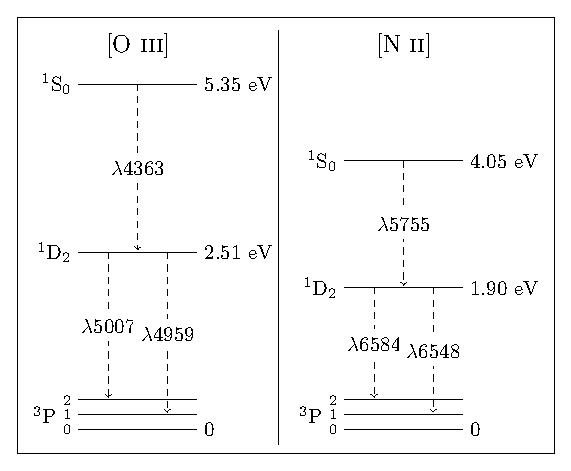
\includegraphics[width=0.5\textwidth]{Images/Paper2/NIIOIII_energy_level_diagram-figure0}
    \caption[{[\ion{O}{3}] and [\ion{N}{2}] energy-level diagram}]{Energy-level 
    diagram for [\ion{O}{3}] and [\ion{N}{2}] $(2p^2)$ ions.  The most important 
    transitions are shown; all are in the visible spectrum.  These forbidden 
    transitions in both oxygen and nitrogen provide an estimate of the electron 
    temperature in the interstellar gas.  Because oxygen is more abundant, we 
    use the oxygen lines to estimate the temperature of the gas.}
    \label{fig:transitions_P2}
\end{figure}


% ------------------------------------------------------------------------------
\subsection{Direct $T_e$ method}

We use the same method to calculate the nitrogen abundance as in Paper I to 
estimate the oxygen abundance.  However, here we use the [\ion{N}{2}] 
$\lambda \lambda 6548, 6584$ doublet instead of the [\ion{O}{2}] $\lambda 3727$ 
and [\ion{O}{3}] $\lambda \lambda 4959,5007$ doublets.  Because the temperature 
estimate depends on the auroral line [\ion{O}{3}] $\lambda 4363$, this method is 
often difficult to employ.  As a result, it works best with low-redshift, 
low-metallicity galaxies.  The electron temperature is derived by solving the 
following system of equations:
\begin{equation}
	t_3 = \frac{1.432}{\log[(\lambda 4959 + \lambda 5007)/\lambda 4363] - \log C_T}
\end{equation}
where $t_3 = 10^{-4} T_e(\text{O}^{++})$ and
\begin{equation}
	C_T = (8.44 - 1.09t_3 + 0.5t_3^2 - 0.08t_3^3)\frac{1 + 0.0004x_3}{1 + 0.044x_3}
\end{equation}
where $x_3 = 10^{-4} n_e t_3^{-0.5}$.  The ionic abundances are then found with 
the equations
\begin{align}
    12 + \log \left( \frac{\text{O}^{++}}{\text{H}^+} \right) &= \log \frac{\lambda 4959 + \lambda 5007}{\text{H}\beta} + 6.200 + \frac{1.251}{t_3} - 0.55\log t_3 - 0.014t_3 \\
	12 + \log \left( \frac{\text{O}^+}{\text{H}^+} \right) &= \log \frac{\lambda 3727}{\text{H}\beta} + 5.961 + \frac{1.676}{t_2} - 0.40\log t_2 - 0.034t_2 + \log (1+1.35x_2) \\
	12 + \log \left( \frac{\text{N}^+}{\text{H}^+} \right) &= \log \frac{\lambda 6548 + \lambda 6584}{\text{H}\beta} + 6.234 + \frac{0.950}{t_2} - 0.42\log t_2 - 0.027t_2 + \log (1 + 0.116x_2)
\end{align}
where $t_2 = 10^{-4} T_e(\text{O}^+)$ and $x_2 = 10^{-4} n_e t_2^{-0.5}$.  We 
assume that $T_e(\text{N}^+) = T_e(\text{O}^+)$.

The signal-to-noise ratio of the SDSS spectra is too low to directly estimate 
the temperature of the gas in the low-ionization zone.  As a result, we use the 
relation $t_2 = 0.7t_3 + 0.3$ by \cite{Garnett92}.  This relation has been shown 
to overestimate this temperature \citep{Andrews13}.  Since the metal emission 
lines are the primary method of cooling for the gas, a high temperature 
corresponds to a low metallicity.  Therefore, an overestimate of the temperature 
results in an underestimated abundance.  As shown in Paper I, this only affects 
perhaps 15 of the dwarf galaxies in our sample and does not influence our 
conclusions.

The sum of the abundances of each of the element's ionization states is equal to 
the total abundance of any element, whether or not all ionization states are 
observed.  Most of oxygen exists as either singly or doubly ionized, so the 
total oxygen abundance is
\begin{equation}
	\frac{\text{O}}{\text{H}} = \frac{\text{O}^{++}}{\text{H}^+} + \frac{\text{O}^+}{\text{H}^+}
\end{equation}
Since we can only observe the nitrogen abundance in one of the main ionization 
states, we use an ionization correction factor (ICF) to account for the missing 
states.  For any element X, the total abundance is 
\begin{equation}\label{eqn:ICF}
    \frac{\text{X}}{\text{H}} = \sum_i ICF_i \frac{\text{X}^i}{\text{H}}
\end{equation}
For nitrogen, we employ the ICFs as defined in \cite{Izotov06}:
\begin{equation}\label{eqn:ICF_N}
    ICF(\text{N}^+) = \left\{ \begin{array}{ll}
    -0.825v + 0.718 + \frac{0.853}{v} & \mbox{low $Z$}\\
    -0.809v + 0.712 + \frac{0.852}{v} & \mbox{intermed $Z$}\\
    1.467v + 1.752 + \frac{0.688}{v} & \mbox{high $Z$}
    \end{array} \right.
\end{equation}
where $v = \text{O}^+ / (\text{O}^+ + \text{O}^{++})$.  The range for low $Z$ 
covers galaxies with $12 + \log \left( \text{O}/\text{H} \right) \leq 7.2$, 
while high $Z$ includes galaxies with 
$12 + \log \left( \text{O}/\text{H} \right) \geq 8.2$.  For galaxies with 
$7.2 < 12 + \log \left( \text{O}/\text{H} \right) < 7.6$, the values for the 
ICFs are a linear interpolation between the low-$Z$ and intermediate-$Z$ values, 
while the ICFs for galaxies with 
$7.6 < 12 + \log \left( \text{O}/\text{H} \right) < 8.2$ are a linear 
interpolation between the intermediate-$Z$ and high-$Z$ values.

The N/O ratio can be found from the O/H and N/H ratios:
\begin{equation}\label{eqn:NO}
    \log \left(\frac{\text{N}}{\text{O}}\right) = \left[ 12 + \log \left( \frac{\text{N}}{\text{H}} \right) \right] - \left[ 12 + \log \left( \frac{\text{O}}{\text{H}} \right) \right]
\end{equation}

%The N$^+$/O$^+$ ratio can then be found from the O$^+$/H and N$^+$/H ratios:
%\begin{equation}
%    \log \left(\frac{\text{N}^+}{\text{O}^+}\right) = \left[ 12 + \log \left( \frac{\text{N}^+}{\text{H}^+} \right) \right] - \left[ 12 + \log \left( \frac{\text{O}^+}{\text{H}^+} \right) \right]
%\end{equation}




%%%%%%%%%%%%%%%%%%%%%%%%%%%%%%%%%%%%%%%%%%%%%%%%%%%%%%%%%%%%%%%%%%%%%%%%%%%%%%%%
%
%    DATA
%
%%%%%%%%%%%%%%%%%%%%%%%%%%%%%%%%%%%%%%%%%%%%%%%%%%%%%%%%%%%%%%%%%%%%%%%%%%%%%%%%
\section[Data]{SDSS data and galaxy selection}

The SDSS Data Release 7 \citep[DR7;][]{Abazajian09} uses drift scanning to map 
approximately one-quarter of the northern sky; it is a wide-field multiband 
imaging and spectroscopic survey.  A dedicated 2.5 m telescope at the Apache 
Point Observatory in New Mexico \citep{Fukugita96, Gunn98} takes the photometric 
data in the five-band SDSS system --- $u$, $g$, $r$, $i$, and $z$.  Galaxies 
selected for spectroscopic analysis must have a Petrosian $r$-band magnitude 
$m_r < 17.77$ \citep{Lupton01, Strauss02}.  Two double fiber-fed spectrographs 
and fiber plug plates take the spectra in an observed wavelength range of 
3800--9200 \AA with a resolution $\lambda / \Delta \lambda \sim 1800$ and a 
minimum fiber separation of 55" \citep{Blanton03}.  As in Paper I, we use 
the emission-line flux data from the MPA-JHU value-added catalog, which is based 
on the SDSS DR7 sample of galaxies.  Total star formation rates and total 
specific star formation rates are also from the MPA-JHU value-added catalog, 
following the technique discussed in \cite{Brinchmann04}.  The MPA-JHU catalog 
is also the source of the stellar mass estimates used, as calculated in 
\cite{Tremonti04}, following the method outlined in \cite{Kauffmann03}.  The 
KIAS value-added galaxy catalog \citep{Choi10} is our source of the absolute 
magnitudes and colors of the galaxies.


%-------------------------------------------------------------------------------
\subsection{Spectroscopic selection}\label{sec:SDSS_limits}

The following requirements are implemented on the SDSS DR7 main spectroscopic 
galaxy sample described above.  We use the same requirements for our sample as 
in Paper I; all galaxies must have
\begin{enumerate}
    \item{$M_r > -17$ (dwarf galaxies);}
    \item{a minimum $5\sigma$ detection of H$\beta$;}
    \item{a minimum $1\sigma$ detection of [\ion{O}{3}] $\lambda 4363$;}
    \item{a flux $>0$ for all other required lines;}
    \item{$T_e (\text{\ion{O}{3}}) < 3\times 10^4 \text{ K}$;}
    \item{a star-forming BPT classification by \cite{Brinchmann04}.}
\end{enumerate}
We also use the \texttt{oii\_flux} value from the MPA-JHU catalog in place of 
their [\ion{O}{2}] $\lambda \lambda 3726, 3729$ flux measurement since we are 
working at such low redshifts ($0.02 < z < 0.03$).  Detailed descriptions of 
these criteria can be found in Section 3.1 of Paper I.


%-------------------------------------------------------------------------------
\subsection{Void classification}

The large-scale environment of the galaxies was determined using the void 
catalog constructed by \cite{Pan12}, which is based on the galaxies in the SDSS 
DR7 catalog.  The VoidFinder algorithm of \cite{Hoyle02} removes all isolated 
galaxies with absolute magnitudes $M_r < -20$ (a galaxy is defined to be 
isolated if its third nearest neighbor is more than 7 $h^{-1}$ Mpc away).  
Placing a grid over the remaining galaxies, VoidFinder grows spheres in the 
centers of all grid cells that contain no galaxies.  The spheres expand until 
they encounter four galaxies on the surface.  To be considered part of a void, a 
sphere must have a minimum radius of 10 Mpc; two spheres that overlap by more 
than 10\% are considered part of the same void.  We refer the reader to 
\cite{Hoyle02} for a more detailed description of the VoidFinder algorithm.  
Using these voids, galaxies that live within any void sphere are classified as 
a void galaxy; those that are outside the spheres are considered wall galaxies.  
Due to the construction of the void spheres, we cannot identify any voids within 
10 Mpc of the edge of the survey.  As a result, the large-scale environment of 
any galaxy within this boundary is uncertain.

9519 of the $\sim$800,000 galaxies with spectra available in SDSS DR7 are dwarf 
galaxies ($M_r > -17$).  42 void dwarf galaxies, 89 wall dwarf galaxies, and 4 
dwarf galaxies with uncertain large-scale environments are left to analyze after 
applying the spectroscopic cuts (or 135 dwarf galaxies in total, 131 of which 
are used in the environmental study).


%%%%%%%%%%%%%%%%%%%%%%%%%%%%%%%%%%%%%%%%%%%%%%%%%%%%%%%%%%%%%%%%%%%%%%%%%%%%%%%%
%
%    ANALYSIS & RESULTS
%
%%%%%%%%%%%%%%%%%%%%%%%%%%%%%%%%%%%%%%%%%%%%%%%%%%%%%%%%%%%%%%%%%%%%%%%%%%%%%%%%
\section[Results]{Abundance analysis and results}

Our primary objective is to perform a relative measurement of the N/O ratio of 
dwarf galaxies to discern how the large-scale environment affects their chemical 
evolution.  As discussed in Paper I, multiple methods have been developed for 
metallicity calculations based on the quality of the spectra.  We use only the 
direct $T_e$ method for our abundance calculations, due to the limited galaxy 
types used in the calibration or theoretical development of other methods.

For reference, the solar metallicity $Z_{\odot} = 8.69\pm 0.05$ 
\citep{Asplund09}.


%-------------------------------------------------------------------------------
\subsection{Estimation of uncertainties and comparison of N/O and N$^+$/O$^+$}

% Uncertainties
We estimate uncertainties in the computed abundances using a Monte Carlo method.  
We calculate 100,000 abundance estimates using the measured line fluxes and 
scaled uncertainty estimates.  A new positive ``fake'' line flux is drawn from a 
normal distribution for each abundance estimate.  The standard deviation in 
the sets of 100,000 calculated abundance values is used for the error in the 
abundance calculation.  A more in-depth description of this process can be found 
in Paper I.

It has been common practice to assume that N/O $\cong$ N$^+$/O$^+$, thus 
eliminating the need for the ICF in Eqn. \ref{eqn:ICF}.  We find that this is a 
reasonable but slightly biased approximation, agreeing with the results of 
\cite{Nava06}.  A comparison of the N/O ratio and the N$^+$/O$^+$ ratio for our 
set of dwarf galaxies can be seen in Fig. \ref{fig:NO_NpOp}; galaxies with 
absolute magnitudes $M_r > -20$ are shown in gray for context.  A linear fit to 
all star-forming galaxies with magnitudes $M_r > -20$ has a slope of only 
$0.927\pm 0.0018$, with an rms error of 0.032 for the fit.  This comparison 
indicates that lower values of the N$^+$/O$^+$ ratio underestimate the N/O 
ratio, while higher values of N$^+$/O$^+$ overestimate the N/O ratio.  
Throughout this paper, we study the N/O ratio using ICF-corrected estimates of 
N/O (Eqns. \ref{eqn:ICF_N} and \ref{eqn:NO}).

\begin{figure}
    \centering
    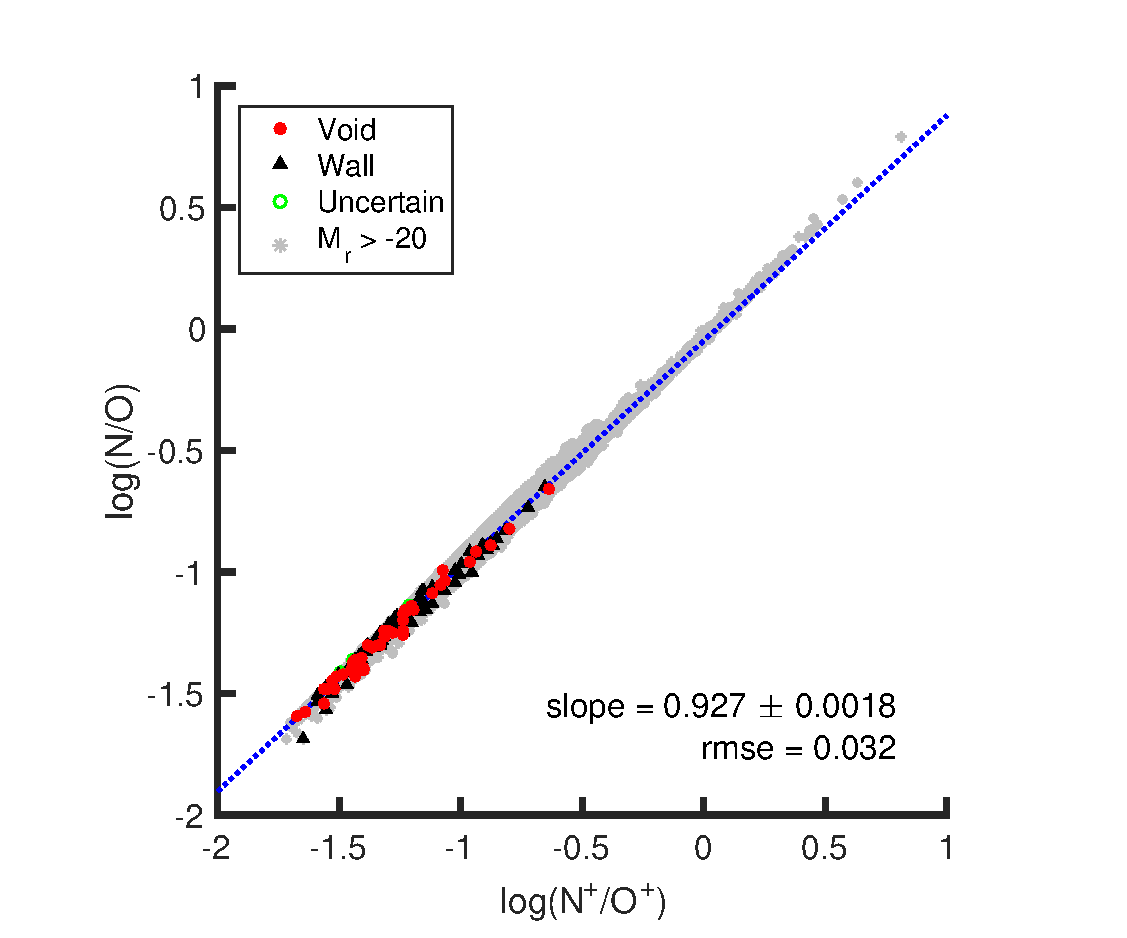
\includegraphics[width=0.5\textwidth]{Images/Paper2/1sig_I06_dwarf_0-20_SF_t3_logNpOp_logNO_fit}
    \caption[N/O versus N$^+$/O$^+$]{Comparison of the N/O and N$^+$/O$^+$ 
    abundance ratios for our dwarf galaxies.  Brighter galaxies ($M_r > -20$) 
    are shown in gray for context.  All our star-forming galaxies with 
    $M_r > -20$ roughly follow the approximation that N/O $\cong$ N$^+$/O$^+$, 
    which is often assumed in other studies of the abundance ratio of nitrogen 
    to oxygen.  In this paper, we will be using the abundance ratio N/O for our 
    analysis.}
    \label{fig:NO_NpOp}
\end{figure}


%-------------------------------------------------------------------------------
\subsection{Sources of systematic error}

There is a radial dependence of many physical properties of galaxies 
\citep{Bell00}.  Consequently, abundance estimates may depend on the locations 
of the spectroscopic fiber on the galaxy.  If all of the galaxy's light is not 
contained within the fiber of the spectrograph, the estimated abundances will 
not necessarily be representative of global abundance values.  For example, 
\cite{Bell00} show that the metallicity is not constant throughout a galaxy.  
Due to the spatially resolved spectra produced by MaNGA of SDSS-IV 
\citep{SDSS13}, a statistically significant measure of the radial dependence of 
a galaxy's metallicity should soon be possible \citep{Wilkinson15}.  In SDSS 
DR7, the fiber diameter is 3", corresponding to a physical diameter between 1.29 
and 1.93 kpc at redshifts $0.02 < z < 0.03$.  This covers a majority of most 
dwarf galaxies' luminous surfaces.  The fiber is almost always placed on the 
brightest spot of the galaxy, which is often the center of the galaxy for spiral 
and ellipticals.  Since the metallicity has been shown to decrease at large 
radius, these abundance values may be overestimates of the global abundances.  
Since many dwarf galaxies are irregular galaxies, the fiber is instead focused 
on a bright \ion{H}{2} region.  As a result, we are estimating the abundances of 
the gas from which stars recently formed.

We are implicitly limiting our sample of galaxies to only blue, star-forming 
dwarf galaxies as a result of our selection criteria outlined in Section 
\ref{sec:SDSS_limits}.  Consequently, this is not a representative sample of the 
full dwarf galaxy population.  In this study we are only able to discuss the 
large-scale environmental influence on blue, star-forming dwarf galaxies within 
a narrow redshift range.  It is impossible to use the direct $T_e$ method to 
measure the chemical abundances of red dwarf galaxies because the UV photons 
from young stars are needed to excite the interstellar gas.


%-------------------------------------------------------------------------------
\subsection{Galaxy abundances}

Abundances estimated using the direct $T_e$ method for our dwarf galaxy sample 
are listed in Table \ref{tab:Results_P2}, along with other important 
characteristics and identification for the galaxies (including their large-scale 
environment classification).

% Results table
\begin{sidewaystable}
\centering

\begin{tabular}{cccccccccccc}
Index\footnote{KIAS-VAGC galaxy index number} & R.A. & Decl. & Redshift & $M_r$ & \multicolumn{2}{c}{$12 + \log \left( \frac{\text{O}}{\text{H}} \right)$} & \multicolumn{2}{c}{$12 + \log \left( \frac{\text{N}}{\text{H}} \right)$} & \multicolumn{2}{c}{$\log \left( \frac{\text{N}}{\text{O}} \right)$} & Void/Wall \\
\hline \\
63713 & \RA{09}{20}{04}{.27} & -\dec{00}{30}{08}{.97} & 0.0257 & -16.73 & 7.80 & $\pm$0.41 & 6.83 & $\pm$0.28 & -0.97 & $\pm$0.49 & Wall \\
73537 & \RA{09}{25}{24}{.23} & +\dec{00}{12}{40}{.39} & 0.0250 & -16.94 & 7.94 & $\pm$0.34 & 6.76 & $\pm$0.24 & -1.18 & $\pm$0.41 & Wall \\
75442 & \RA{13}{13}{24}{.25} & +\dec{00}{15}{02}{.95} & 0.0264 & -16.81 & 7.55 & $\pm$0.35 & 6.73 & $\pm$0.24 & -0.82 & $\pm$0.42 & Void \\
168874 & \RA{11}{45}{13}{.16} & -\dec{01}{48}{17}{.68} & 0.0273 & -16.99 & 8.16 & $\pm$0.31 & 6.94 & $\pm$0.21 & -1.21 & $\pm$0.37 & Wall \\
184308 & \RA{09}{39}{09}{.38} & +\dec{00}{59}{04}{.15} & 0.0244 & -16.73 & 7.36 & $\pm$0.43 & 6.71 & $\pm$0.31 & -0.65 & $\pm$0.53 & Wall\\
\end{tabular}

\caption[Chemical abundances of subset of 135 dwarf galaxies]{Five of the 135 dwarf galaxies analyzed from SDSS DR7.  The flux values for all required emission lines can be found in the MPA-JHU value-added catalog.  Metallicity values are calculated using the direct $T_e$ method, with error estimates via a Monte Carlo method.  The void catalog of \cite{Pan12} is used to classify the galaxies as either Void or Wall.  If a galaxy is located too close to the boundary of the SDSS to identify whether or not it is inside a void, it is labeled as Uncertain.  (This table is available in its entirety in machine-readable form.)}

\label{tab:Results_P2}

\end{sidewaystable}



%-------------------------------------------------------------------------------
\subsubsection{Oxygen and nitrogen abundances}\label{sec:OH_NH}

Histograms of the resulting oxygen and nitrogen abundances are shown in Figs. 
\ref{fig:met1sig} and \ref{fig:N_1sig}, respectively.  Both figures show very 
little difference in the distribution of abundance values in dwarf galaxies 
between voids and walls.  A two-sample Kolmogorov-Smirnov (K-S) test quantifies 
this observation --- it produced a test statistic of 0.13 for oxygen and 0.11 
for nitrogen, corresponding to a probability of 67.1\% and 83.8\%, respectively, 
that a test statistic greater than or equal to this calculated test statistic 
will be measured if the void sample were drawn from the wall sample.  The 
cumulative distribution function (CDF) of these samples can be seen in the right 
panel of Figures \ref{fig:met1sig} and \ref{fig:N_1sig}.  The K-S test 
quantifies the visual impression in these figures that the distributions of 
oxygen and nitrogen abundances are similar for dwarf galaxies in voids and 
walls.

The average and median values of the dwarf galaxy abundances indicate very 
little large-scale environmental influence on the oxygen and nitrogen 
abundances.  The average oxygen abundance for void dwarf galaxies is 
$7.99\pm 0.049$ and the median is 8.04, while the average for wall dwarf 
galaxies is $7.93\pm 0.036$ with a median value of 8.01.  This implies that the 
wall dwarf galaxies have lower oxygen abundances by an average of 
$0.07\pm 0.060$ relative to the void dwarf galaxies; the shift in the median 
values is 0.03 for the dwarf galaxies, with wall dwarf galaxies having lower 
oxygen abundances than void dwarf galaxies.  There is a also a shift in the 
nitrogen abundances for the dwarf galaxies: void dwarf galaxies have an average 
nitrogen abundance of $6.74\pm 0.035$ and a median of 6.77, while the wall dwarf 
galaxies have an average nitrogen abundance of $6.72\pm 0.025$ and a median of 
6.75.  Again, wall dwarf galaxies have, on average, $0.02\pm 0.043$ lower 
nitrogen abundances than the void dwarf galaxies (the median shift for the 
nitrogen abundance of dwarf galaxies is 0.01, with wall galaxies lower than void 
dwarf galaxies).  These shifts are within the uncertainty, so they are not 
statistically significant --- if there is a large-scale environmental influence 
on the abundances of oxygen and nitrogen relative to hydrogen in dwarf galaxies, 
it is small.

% Dwarf galaxies
%\begin{figure*}
%    \centering
%    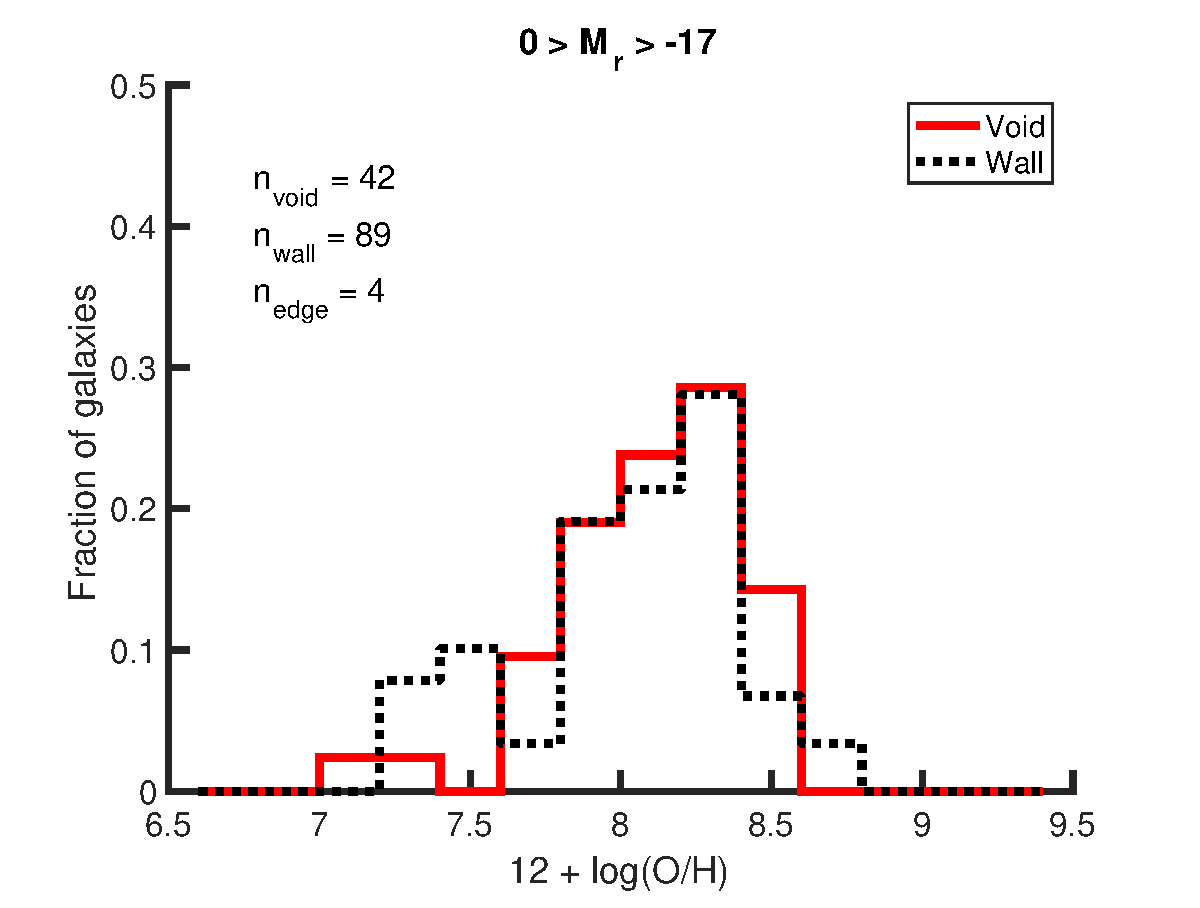
\includegraphics[width=0.49\textwidth]{Images/Paper1/1sig_dwarf_SF_t3_12logOH_hist}
%    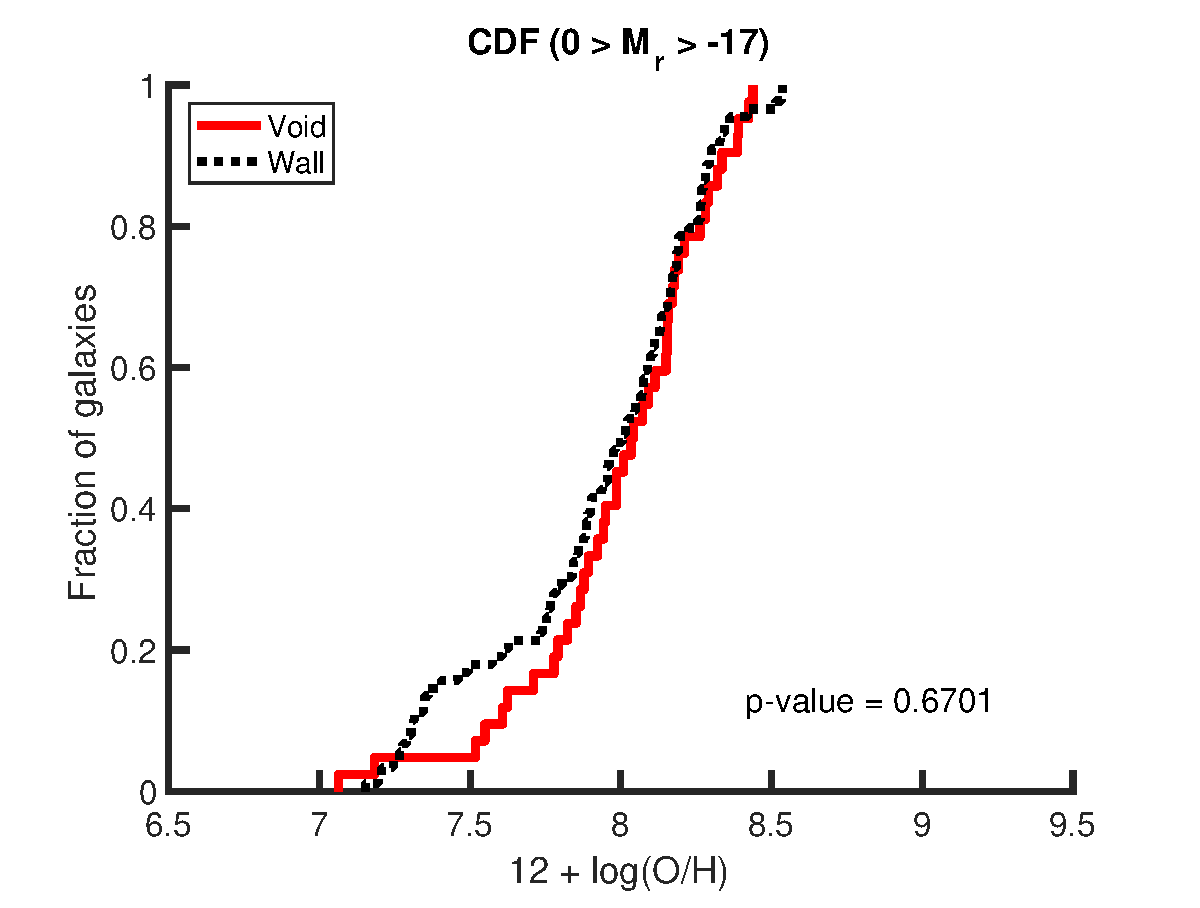
\includegraphics[width=0.49\textwidth]{Images/Paper1/1sig_dwarf_SF_t3_12logOH_CDF}
%    \caption{Gas-phase oxygen abundances (relative to hydrogen) of void dwarf 
%    (red solid line) and wall dwarf (black dashed line) galaxies, taken from 
%    Fig. 4 in Paper I.  As we demonstrate in Paper I, the gas-phase oxygen 
%    abundances in dwarf galaxies do not depend on the large-scale environment.}
%    \label{fig:met1sig}
%\end{figure*}

\begin{figure*}
    \centering
    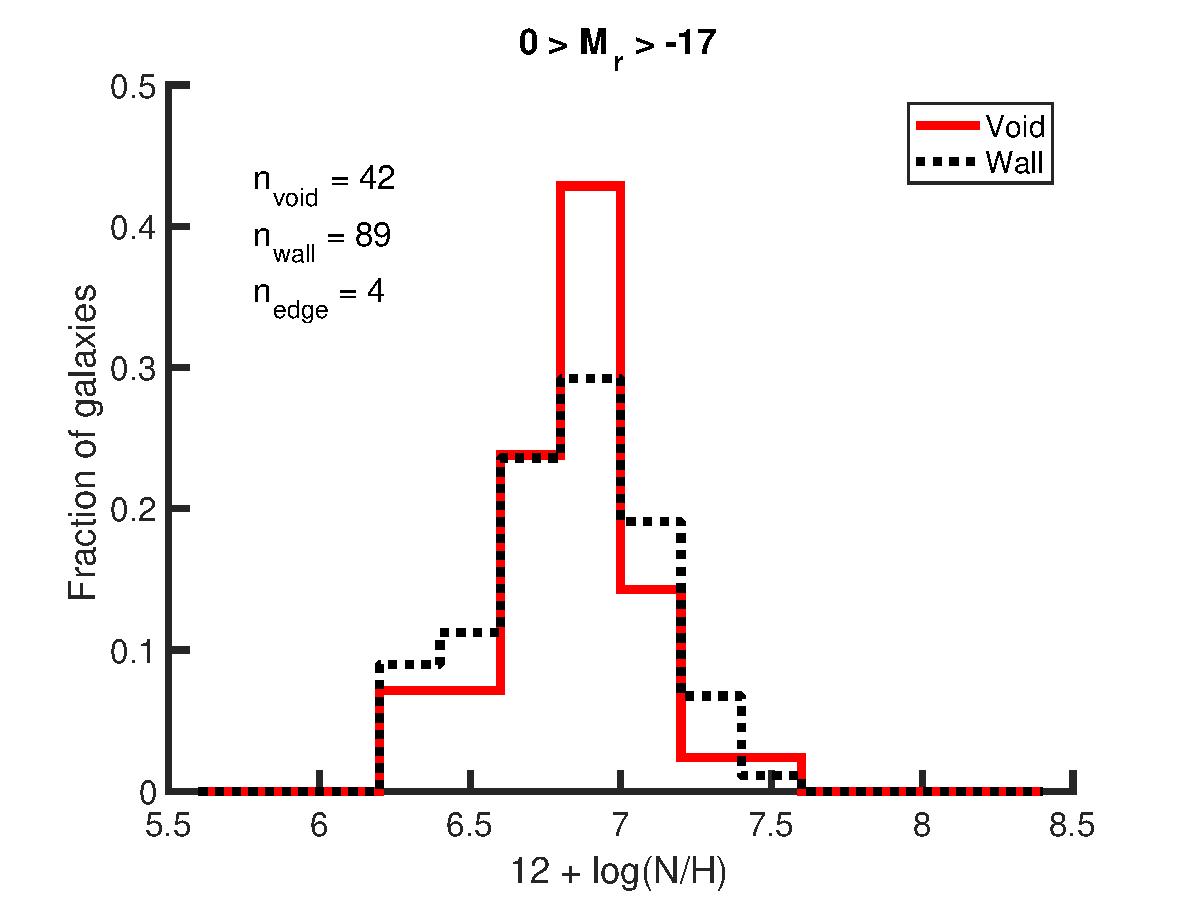
\includegraphics[width=0.49\textwidth]{Images/Paper2/1sig_dwarf_SF_t3_12logNH_hist}
    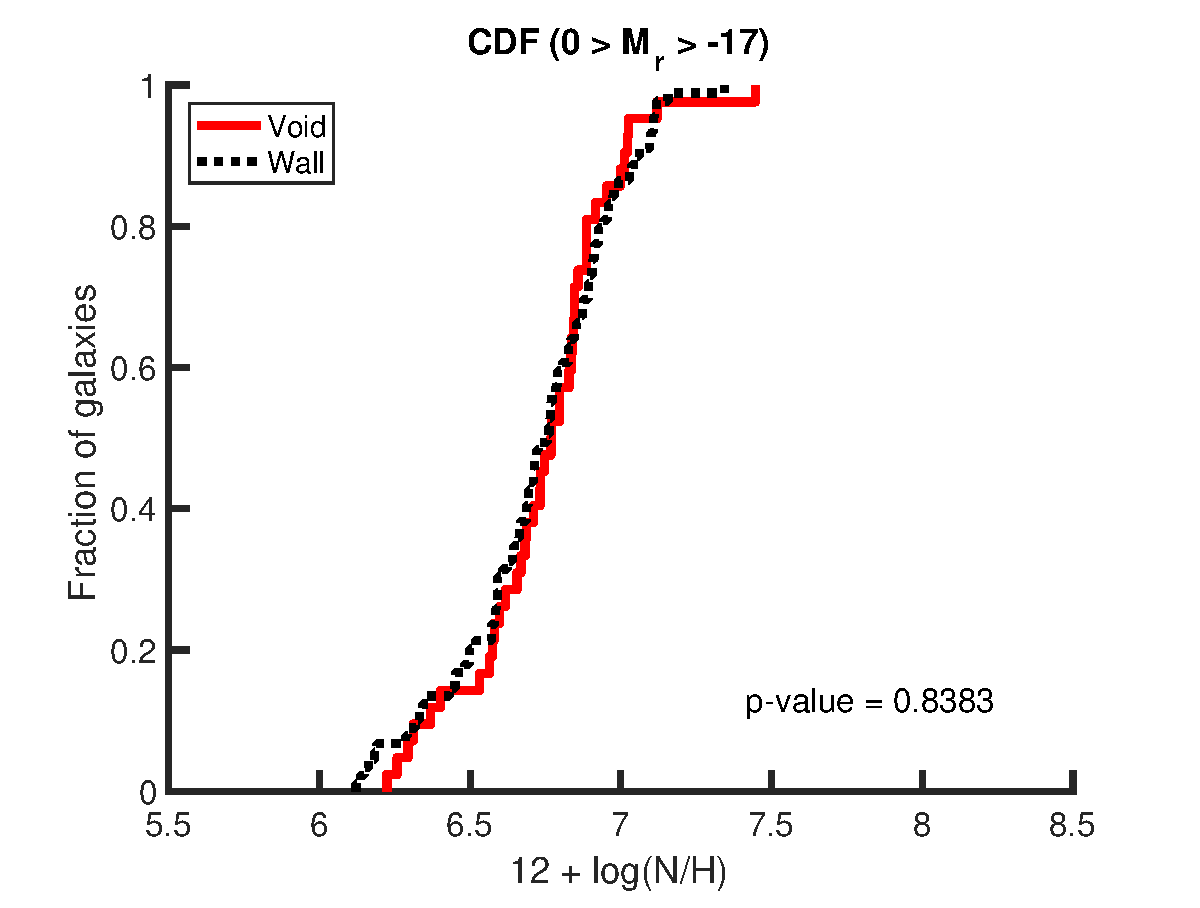
\includegraphics[width=0.49\textwidth]{Images/Paper2/1sig_dwarf_SF_t3_12logNH_CDF}
    \caption[Nitrogen distribution of 135 dwarf galaxy sample]{Abundance of 
    nitrogen relative to hydrogen of void dwarf (red solid line) and wall dwarf 
    (black dashed line) galaxies.  A two-sample K-S test of the two data sets 
    results in an asymptotic $p$-value of 0.84, indicating an 84\% probability 
    that a test statistic greater than the observed value of 0.11 will be seen 
    if the void sample is drawn from the wall sample.  This is reflected 
    visually, as there appears to be very little difference between the two 
    populations, indicating that there is little large-scale environmental 
    influence on the nitrogen abundance of dwarf galaxies.}
    \label{fig:N_1sig}
\end{figure*}

%%%% Brighter star-forming galaxies %%%%%%%%%%%%%%%%%%%%%%%%%%%%%%%%%%%%%%%%%%%%
To see how our results of the environmental dependence of dwarf galaxies compare 
with somewhat brighter galaxies, we perform the same analysis on galaxies with 
absolute magnitudes $-17 > M_r > -20$.  The results of this analysis can be seen 
in Figs. \ref{fig:Z_bright} and \ref{fig:N_bright}.  As the dwarf galaxies have 
already shown, there is no obvious large-scale environmental dependence of the 
oxygen and nitrogen abundances of these brighter galaxies.  The results of a 
two-sample K-S test (listed in Table \ref{tab:stats}) mostly support this 
conclusion.  In the brightest magnitude bin (galaxies with $-19 > M_r > -20$), 
the K-S test returns a $p$-value of only 0.00062 for the oxygen abundances, 
indicating only a 0.062\% chance that there will be a test statistic greater 
than 0.07 if the void sample is drawn from the wall sample.  The oxygen 
abundances for void galaxies are higher than the wall galaxies by an average of 
$0.04\pm 0.017$ in this absolute magnitude bin, reinforcing the results of the 
K-S test that there is a large-scale environmental influence on the oxygen 
abundance in galaxies with magnitudes $-19 > M_r > -20$.  While the results of 
the K-S test are not as convincing for this magnitude range in the nitrogen 
abundances, there is still an average shift of $0.02\pm 0.011$ toward higher 
nitrogen abundances for void galaxies.  While only one magnitude bin shows a 
statistically significant shift between the two environments, all magnitude bins 
are shifted in the same direction.  This trend suggests that there may be a mild 
influence on the chemical evolution of galaxies due to their large-scale 
environment.

\begin{figure}
    \centering
    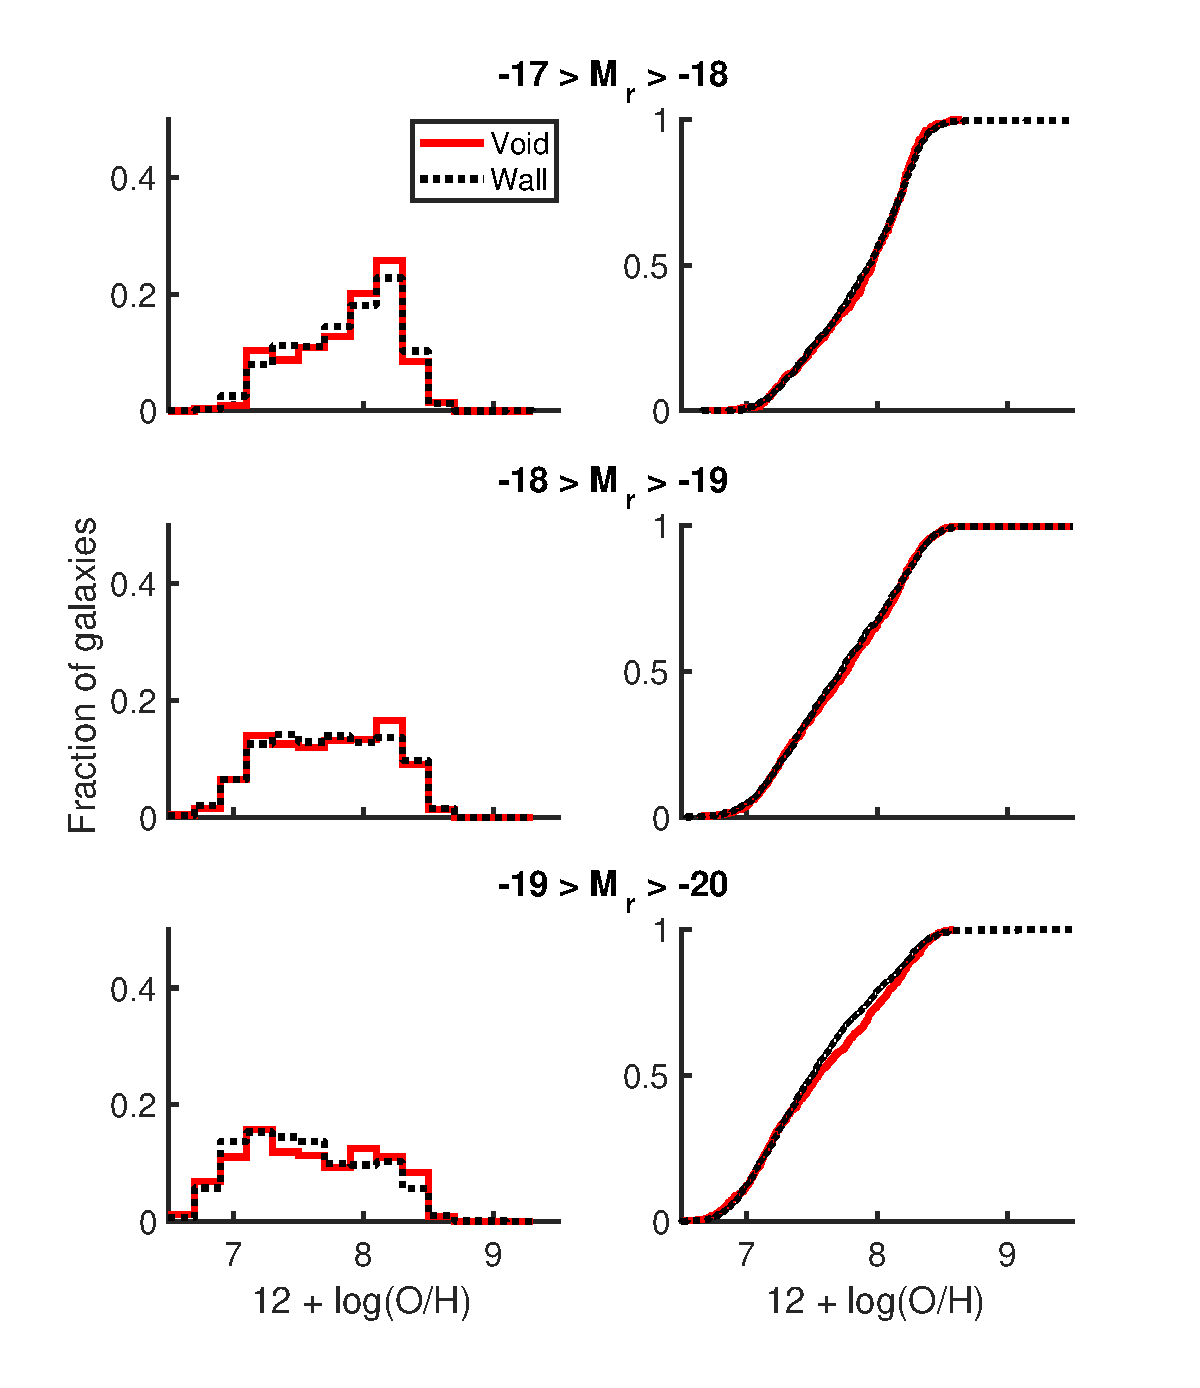
\includegraphics[width=0.75\textwidth]{Images/Paper2/1sig_17-20_SF_t3_12logOH_stacked}
    \caption[Metallicity distribution of star-forming galaxies with 
    $-17 > M_r > -20$]{Gas-phase oxygen abundances relative to hydrogen of void 
    (red solid line) and wall (black dashed line) star-forming galaxies with 
    $-17 > M_r > -18$ (top), $-18 > M_r > -19$ (middle), and $-19 > M_r > -20$ 
    (bottom).  The results of a two-sample K-S test of the two data sets in each 
    absolute magnitude range can be found in Table \ref{tab:stats}.  These 
    results are reflected visually, as there appears to be very little 
    difference between the two populations (regardless of absolute magnitude), 
    indicating that there is little large-scale environmental influence on the 
    oxygen abundance of star-forming galaxies with absolute magnitudes 
    $-17 > M_r > -20$.}
    \label{fig:Z_bright}
\end{figure}

\begin{figure}
    \centering
    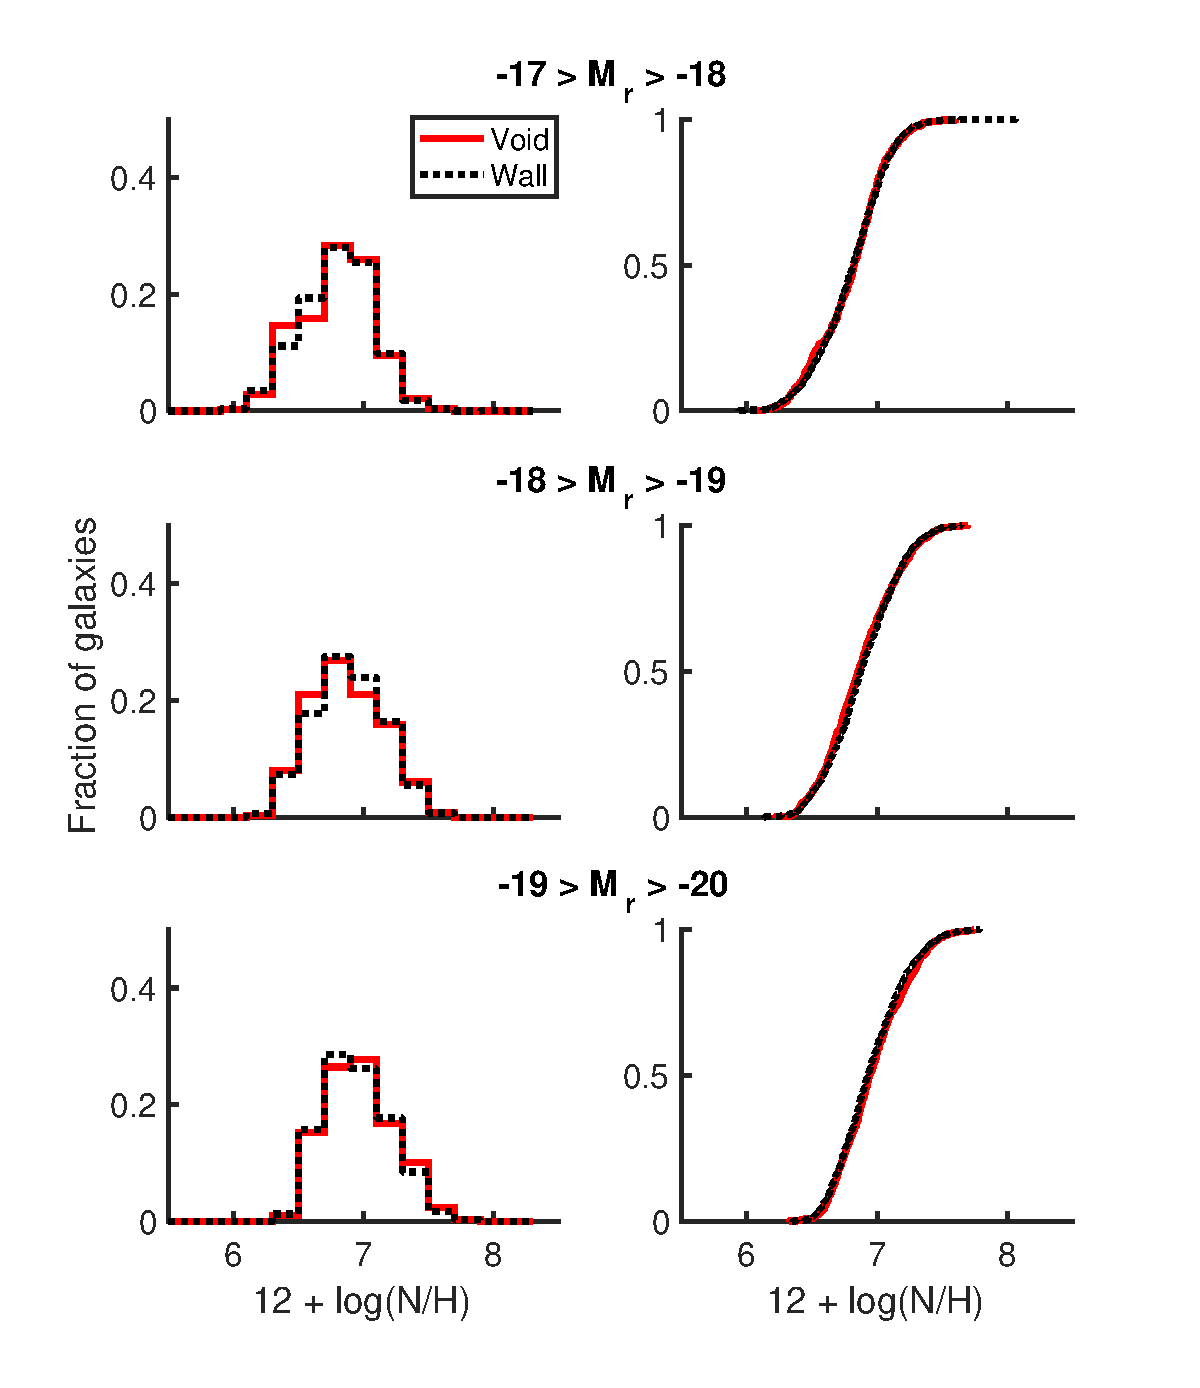
\includegraphics[width=0.75\textwidth]{Images/Paper2/1sig_17-20_SF_t3_12logNH_stacked}
    \caption[Nitrogen distribution of star-forming galaxies with 
    $-17 > M_r > -20$]{Abundance of nitrogen relative to hydrogen of void (red 
    solid line) and wall (black dashed line) star-forming galaxies with 
    $-17 > M_r > -18$ (top), $-18 > M_r > -19$ (middle), and $-19 > M_r > -20$ 
    (bottom).  The results of a two-sample K-S test of the two data sets in each 
    absolute magnitude range can be found in Table \ref{tab:stats}.  These 
    results are reflected visually, as there appears to be very little 
    difference between the two populations (regardless of absolute magnitude), 
    indicating that there is little large-scale environmental influence on the 
    nitrogen abundance of star-forming galaxies with absolute magnitudes 
    $-17 > M_r > -20$.}
    \label{fig:N_bright}
\end{figure}

We note that there appears to be a shift in the oxygen and nitrogen abundances 
between the absolute magnitude bins in Figs. \ref{fig:Z_bright} and 
\ref{fig:N_bright} that is opposite to what is predicted by the mass-metallicity 
relation \citep{Tremonti04}.  This shift toward lower oxygen abundances as the 
galaxies increase in brightness is possibly due to the fact that the metallicity 
estimates are so dependent on the temperature-sensitive [\ion{O}{3}] 
$\lambda 4363$ auroral line.  As galaxies increase in metallicity, this line 
becomes weaker (as its strength is inversely proportional to the temperature).  
If the flux of this line is being underestimated, then the temperature is being 
overestimated, and therefore the oxygen and nitrogen abundances are being 
underestimated.  If we are seeing an underestimate of flux of the [\ion{O}{3}] 
$\lambda 4363$ emission line (and therefore an overestimate of the temperature 
in the region), then we should see a shift toward lower N/H values as the 
absolute magnitude is increased as well.  This pattern can be seen in Fig. 
\ref{fig:N_bright}.

%\begin{table}
%
%    \begin{tabu} in 0.75\textwidth {ccccccccc}
%        Absolute magnitude range & Environment & \# of galaxies & Average & Median & Average shift\footnote[1]{Wall -- Void (Positive shifts indicate that the wall galaxy average is greater than the void average; negative shifts indicate that the void galaxy average is greater than the wall average.)} & Median shift\footnote[1] & $p$-value & KS test statistic \\
%        \hline \\
%        \multirow{2}{*}{Dwarf galaxies} & Void & 42 & $6.74\pm 0.035$ & 6.77 & \multirow{2}{*}{$-0.02\pm 0.043$} & \multirow{2}{*}{0.8383} & \multirow{2}{*}{0.1129}\\
%         & Wall & 89 & $6.72\pm 0.025$ & 6.75 & & & \\
%        \multirow{2}{*}{$-17>M_r>-18$} & Void & 423 & $6.80\pm 0.011$ & 6.82 & \multirow{2}{*}{$0.00\pm 0.014$} & \multirow{2}{*}{0.7364} & \multirow{2}{*}{0.0401}\\
%         & Wall & 895 & $6.80\pm 0.008$ & 6.81 & & & \\
%        \multirow{2}{*}{$-18>M_r>-19$} & Void & 829 & $6.87\pm 0.009$ & 6.85 & \multirow{2}{*}{$0.01\pm 0.011$} & \multirow{2}{*}{0.0873} & \multirow{2}{*}{0.0538}\\
%         & Wall & 1498 & $6.89\pm 0.007$ & 6.87 & & & \\
%        \multirow{2}{*}{$-19>M_r>-20$} & Void & 798 & $6.97\pm 0.009$ & 6.94 & \multirow{2}{*}{$-0.02\pm 0.011$} & \multirow{2}{*}{0.2272} & \multirow{2}{*}{0.0455}\\
%         & Wall & 1490 & $6.95\pm 0.007$ & 6.93 & & & \\
%    \end{tabu}
%
%    \tablecomments{Statistics on the gas-phase nitrogen abundance in void and 
%    wall galaxies in each of the absolute magnitude ranges listed.  Combined 
%    with the histograms in Figs. \ref{fig:N_1sig} and \ref{fig:N_bright}, it is 
%    clear that there is no large-scale environmental dependence of the nitrogen 
%    abundance in galaxies.}
%
%    \label{tab:KStest_N}
%
%\end{table}


%-------------------------------------------------------------------------------
\subsubsection{Ratio of nitrogen to oxygen}

% Dwarf galaxies
In addition to studying the oxygen and nitrogen abundances relative to hydrogen, 
we also look at the ratio of nitrogen to oxygen.  The N/O abundance ratio 
suggests a slightly stronger environmental influence on the chemical evolution 
of dwarf galaxies than the oxygen and nitrogen abundances individually.  As can 
be seen in Fig. \ref{fig:NOratio}, there is a shift in the N/O ratio to lower 
values in the void dwarf galaxies than in the wall dwarf galaxies.  This 
difference is quantified in the K-S test --- the test returned a probability of 
11.1\% that a test statistic greater than or equal to 0.22 will be measured if 
the void sample was drawn from the wall sample.  The void dwarf galaxies have 
lower N/O ratios by an average of $0.05\pm 0.074$ than the wall dwarf galaxies; 
the difference in the median values of the N/O ratio in the void and wall dwarf 
galaxy samples is 0.07.  However, like the shifts seen in the oxygen and 
nitrogen abundances, the shift in the N/O ratio for dwarf galaxies is not 
statistically significant.

\begin{figure*}
    \centering
    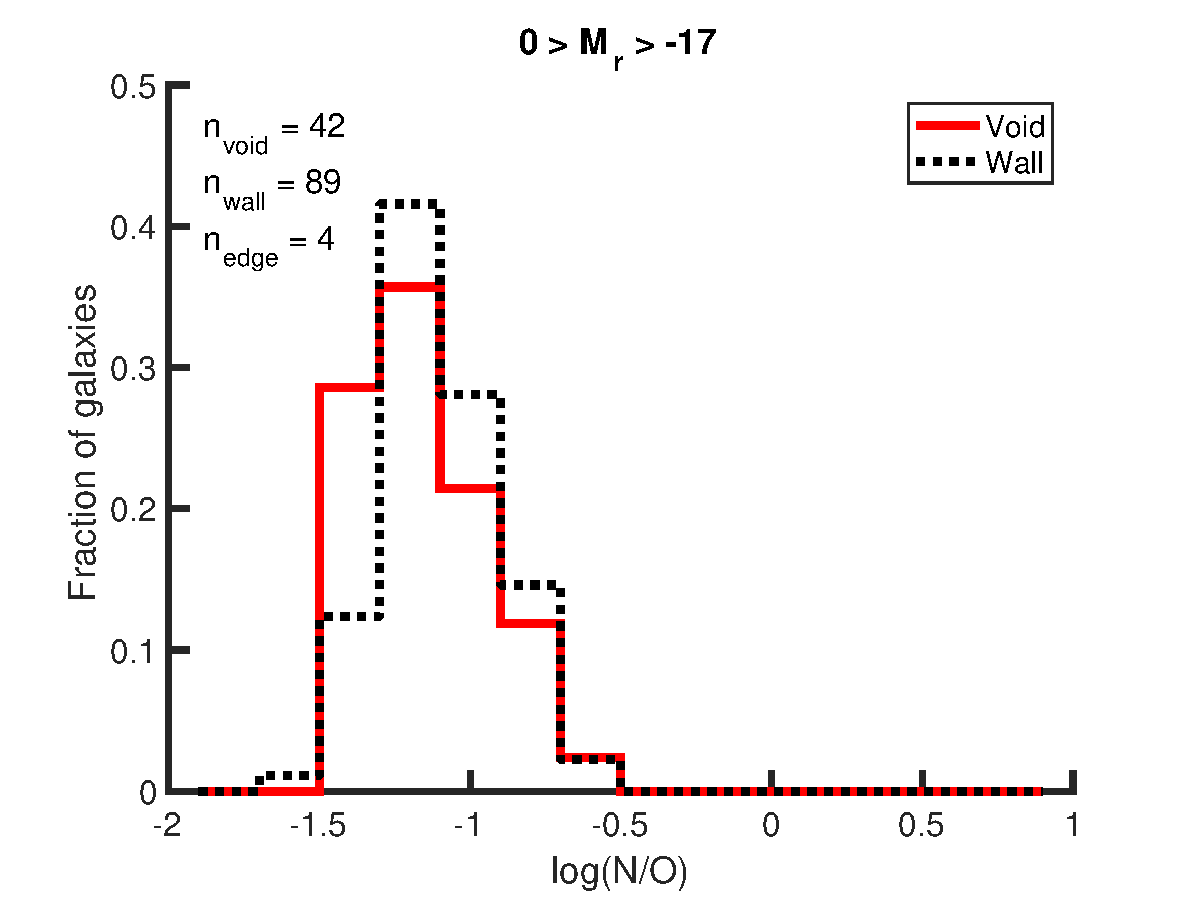
\includegraphics[width=0.49\textwidth]{Images/Paper2/1sig_dwarf_SF_t3_logNO_hist}
    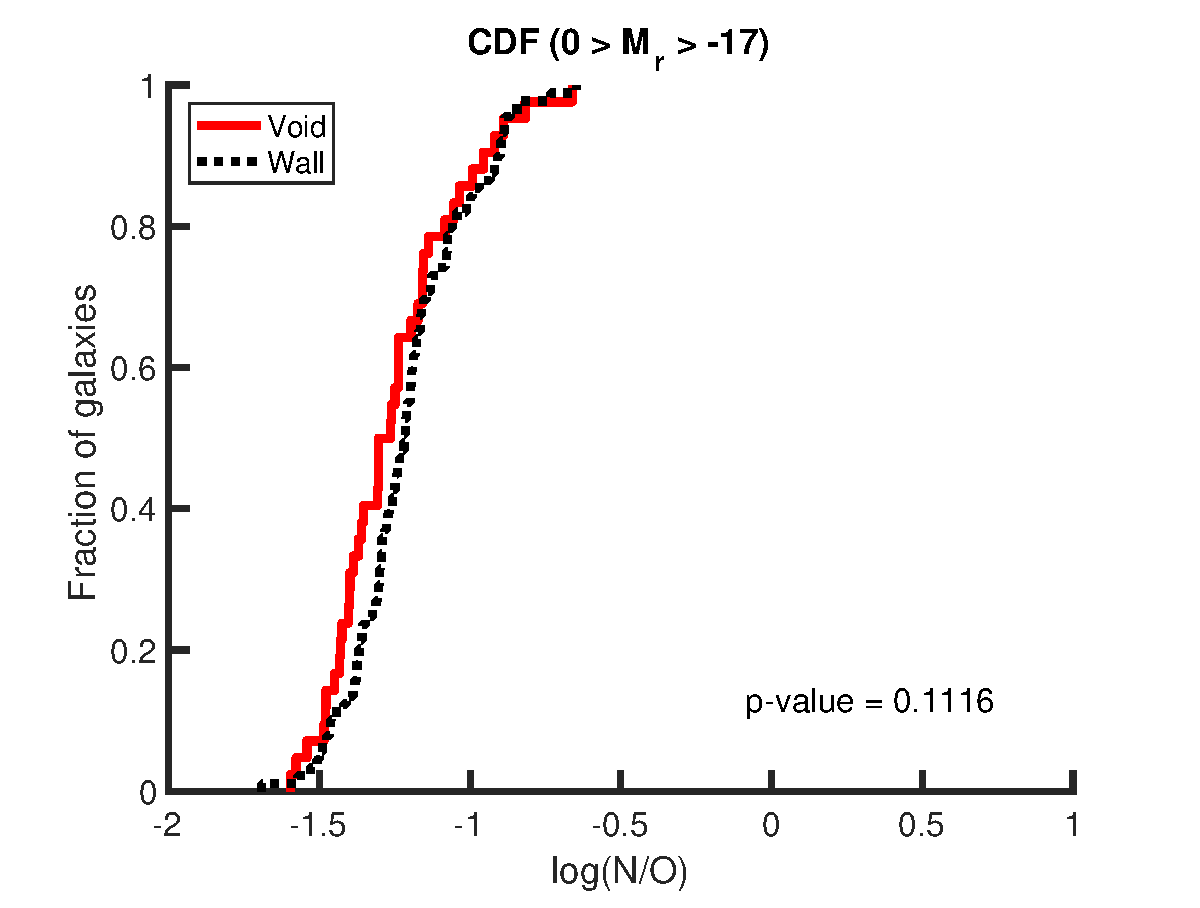
\includegraphics[width=0.49\textwidth]{Images/Paper2/1sig_dwarf_SF_t3_logNO_CDF}
    \caption[N/O distribution of 135 dwarf galaxy sample]{Ratio of nitrogen to 
    oxygen of void dwarf (red solid line) and wall dwarf (black dashed line) 
    galaxies.  A two-sample K-S test of the two data sets results in an 
    asymptotic $p$-value of 0.11, indicating an 11\% probability that a test 
    statistic greater than the observed value of 0.22 will be seen if the void 
    sample was drawn from the wall sample.  This is reflected visually, as the 
    void galaxies appear to have a lower value of N/O than the wall galaxies.  
    This is suggestive of a large-scale environmental influence on the relative 
    chemical abundances in dwarf galaxies.}
    \label{fig:NOratio}
\end{figure*}

%%%% Brighter star-forming galaxies %%%%%%%%%%%%%%%%%%%%%%%%%%%%%%%%%%%%%%%%%%%%
We perform the same analysis with the N/O ratio on somewhat brighter galaxies, 
up through $M_r > -20$; the results of this analysis can be seen in Fig. 
\ref{fig:NO_bright} and in Table \ref{tab:stats}.  The shift toward lower N/O 
ratios for the void galaxies is small for all magnitude bins.  The direction of 
the shift between environments for the N/O ratio is consistent for all absolute 
magnitude bins: void galaxies have slightly lower N/O ratios than wall galaxies.  
This is only very weak evidence of a large-scale environmental influence on the 
relative abundances of elements in galaxies, but it is worth testing for in 
larger samples.

% 17-18
\begin{figure}
    \centering
    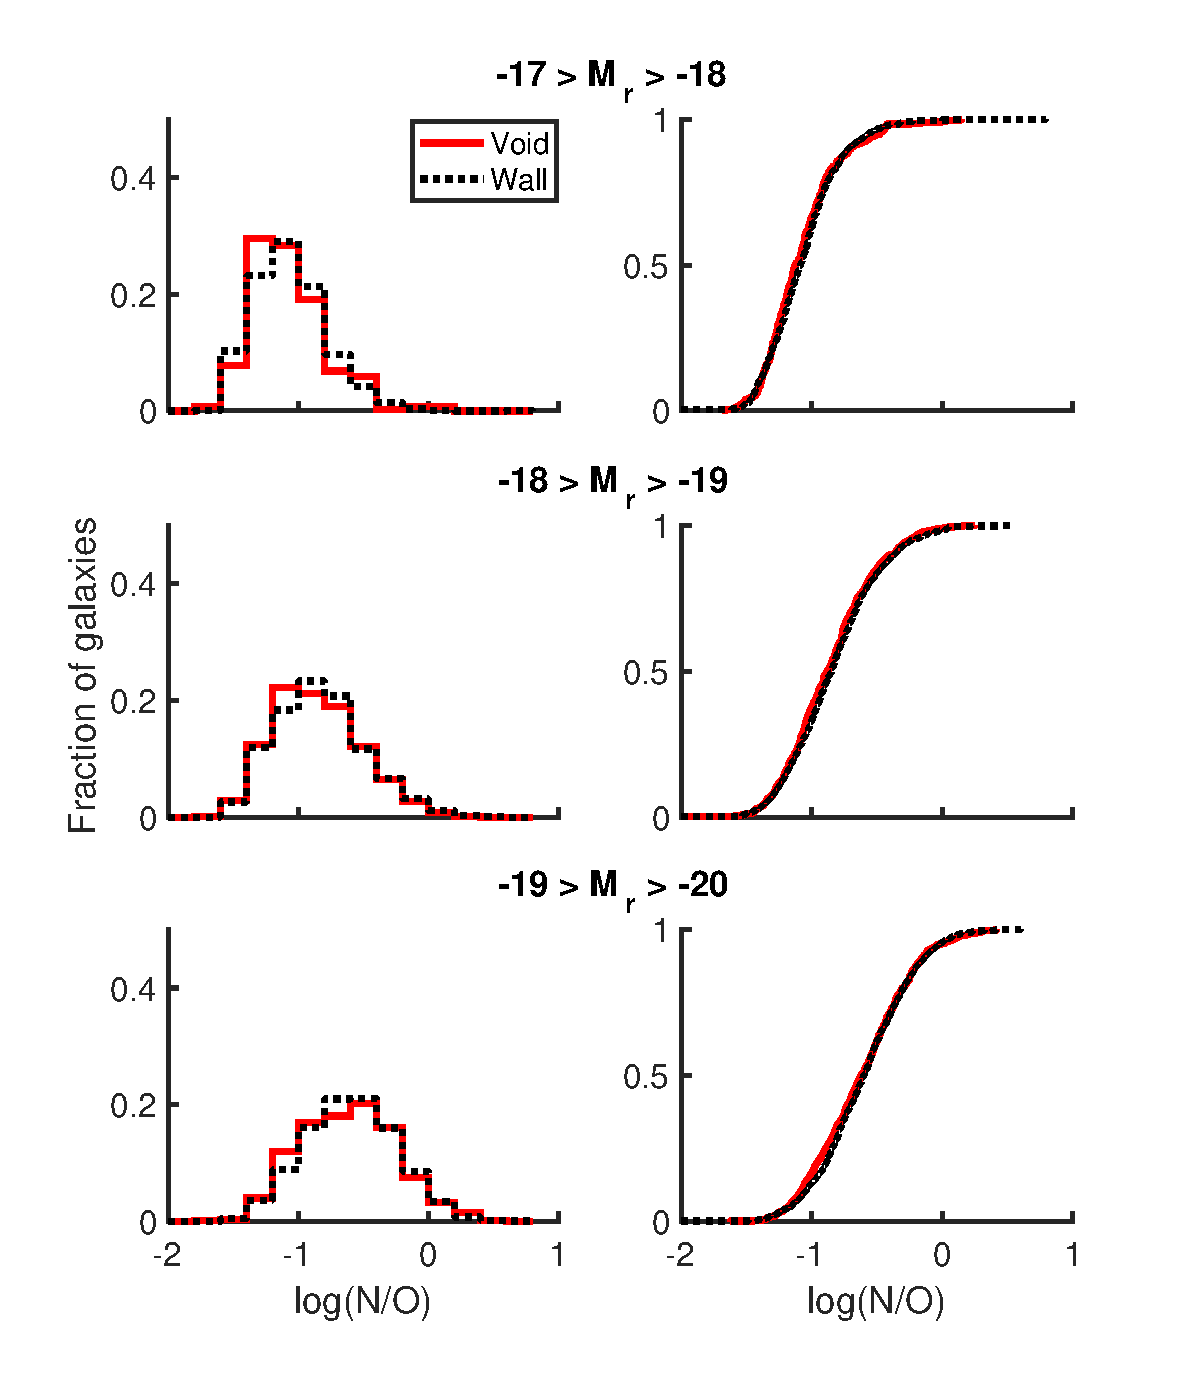
\includegraphics[width=0.75\textwidth]{Images/Paper2/1sig_17-20_SF_t3_logNO_stacked}
    \caption[N/O distribution of star-forming galaxies with $-17 > M_r > -20$]
    {Ratio of nitrogen to oxygen of void (red solid line) and wall (black dashed 
    line) star-forming galaxies with $-17 > M_r > -18$ (top), $-18 > M_r > -19$ 
    (middle), and $-19 > M_r > -20$ (bottom).  The results of a two-sample K-S 
    test of the two data sets in each absolute magnitude range can be found in 
    Table \ref{tab:stats}, in addition to other statistics of the samples.  Both 
    the histograms, CDFs, and statistics suggest a very slight difference 
    between the two populations, indicating a mild large-scale environmental 
    influence on the relative chemical abundances of star-forming galaxies with 
    absolute magnitudes $-17 > M_r > -20$.}
    \label{fig:NO_bright}
\end{figure}

%\begin{table}
%
%    \begin{tabu}{cccccccc}
%        Absolute magnitude range & Environment & \# of galaxies & Average & Median & Average shift\footnote[1]{Wall -- Void (Positive shifts indicate that the wall galaxy average is greater than the void average; negative shifts indicate that the void galaxy average is greater than the wall average.)} & $p$-value & KS test statistic \\
%        \hline \\
%        \multirow{2}{*}{Dwarf galaxies} & Void & 42 & $-1.25\pm 0.060$ & -1.28 & \multirow{2}{*}{$0.05\pm 0.074$} & \multirow{2}{*}{0.1116} & \multirow{2}{*}{0.2191}\\
%         & Wall & 89 & $-1.21\pm 0.044$ & -1.22 & & & \\
%        \multirow{2}{*}{$-17>M_r>-18$} & Void & 423 & $-1.08\pm 0.020$ & -1.13 & \multirow{2}{*}{$-0.00\pm 0.024$} & \multirow{2}{*}{0.2657} & \multirow{2}{*}{0.0588}\\
%         & Wall & 895 & $-1.08\pm 0.014$ & -1.09 & & & \\
%        \multirow{2}{*}{$-18>M_r>-19$} & Void & 829 & $-0.86\pm 0.015$ & -0.88 & \multirow{2}{*}{$0.02\pm 0.019$} & \multirow{2}{*}{0.0763} & \multirow{2}{*}{0.0550}\\
%         & Wall & 1498 & $-0.84\pm 0.012$ & -0.85 & & & \\
%        \multirow{2}{*}{$-19>M_r>-20$} & Void & 798 & $-0.62\pm 0.016$ & -0.62 & \multirow{2}{*}{$0.02\pm 0.020$} & \multirow{2}{*}{0.0715} & \multirow{2}{*}{0.0564}\\
%         & Wall & 1490 & $-0.60\pm 0.012$ & -0.60 & & & \\
%    \end{tabu}
%
%    \caption{Statistics of the relative abundance of nitrogen to oxygen in 
%    void and wall galaxies in each of the absolute magnitude ranges listed.  
%    Combined with the histograms in Figs. \ref{fig:NOratio} and 
%    \ref{fig:NO_bright}, these results suggest that there is a large-scale 
%    environmental dependence of the relative abundance of nitrogen to oxygen in 
%    dwarf galaxies.}
%
%    \label{tab:KStest_NO}
%
%\end{table}

Figure \ref{fig:NO_bright} indicates a shift toward higher values in the peak of 
the N/O distribution as the absolute magnitude of the galaxies increases.  There 
is a known positive correlation between the N/O ratio and the stellar mass of a 
galaxy, as discussed in Sec. \ref{sec:Mass_NO} below.  To test whether this 
relation is causing the shift seen in Figs. \ref{fig:NOratio} and 
\ref{fig:NO_bright}, we downsampled the wall galaxies in each magnitude bin to 
match the void sample.  The original shifts in the N/O ratio seen were still 
present after the downsampling; the observed shift in the N/O ratio is not due 
to any variations in the distribution of the stellar masses between the two 
environments.  In addition, if we are overestimating the temperatures in these 
galaxies as a result of an incorrect measurement of [\ion{O}{3}] $\lambda 4363$ 
(discussed above in Section \ref{sec:OH_NH}), that effect should cancel when we 
look at the ratio of nitrogen to oxygen.  This shift toward higher N/O values as 
a function of absolute magnitude indicates that brighter galaxies produce more 
nitrogen than fainter galaxies (relative to their oxygen abundance).  This 
result is consistent with the theory that nitrogen behaves as a secondary 
element in galaxies with high enough metallicity, if we assume a positive 
correlation between absolute magnitude and metallicity.

\begin{sidewaystable}
\centering

	\begin{tabu} to 0.75\textwidth {ccccccccc}
	    Abs. Mag. Range & Environment & \# of Galaxies & Average & Median & Average Shift\footnote[1]{Wall -- Void (positive shifts indicate that the wall values are greater than the void values; negative shifts indicate that the void values are greater than the wall values)} & Median Shift\footnote[1] & K-S Test Statistic & $p$-value \\
	    \hline
	    \hline
        % Oxygen %%%%%%%%%%%%%%%%%%%%%%%%%%%%%%%%%%%%%%%%%%%%%%%%%%%%%%%%%%%%%%%
        \multicolumn{9}{c}{\OH}\\
        \hline
        \multirow{2}{*}{Dwarf galaxies} & Void & 42 & $7.99\pm 0.049$ & 8.04 & \multirow{2}{*}{$-0.07\pm 0.060$} & \multirow{2}{*}{-0.03} & \multirow{2}{*}{0.1322} & \multirow{2}{*}{0.6701}\\
         & Wall & 89 & $7.93\pm 0.036$ & 8.01 & & & & \\
        \multirow{2}{*}{$-17>M_r>-18$} & Void & 423 & $7.87\pm 0.016$ & 7.96 & \multirow{2}{*}{$0.01\pm 0.020$} & \multirow{2}{*}{-0.02} & \multirow{2}{*}{0.0455} & \multirow{2}{*}{0.5799}\\
         & Wall & 895 & $7.88\pm 0.012$ & 7.94 & & & & \\
        \multirow{2}{*}{$-18>M_r>-19$} & Void & 829 & $7.74\pm 0.013$ & 7.76 & \multirow{2}{*}{$-0.01\pm 0.016$} & \multirow{2}{*}{-0.04} & \multirow{2}{*}{0.0385} & \multirow{2}{*}{0.4000}\\
         & Wall & 1498 & $7.73\pm 0.009$ & 7.73 & & & & \\
        \multirow{2}{*}{$-19>M_r>-20$} & Void & 798 & $7.59\pm 0.013$ & 7.55 & \multirow{2}{*}{$-0.04\pm 0.017$} & \multirow{2}{*}{-0.05} & \multirow{2}{*}{0.0741} & \multirow{2}{*}{0.0062}\\
         & Wall & 1490 & $7.55\pm 0.010$ & 7.50 & & & & \\
        \hline
        % Nitrogen %%%%%%%%%%%%%%%%%%%%%%%%%%%%%%%%%%%%%%%%%%%%%%%%%%%%%%%%%%%%
        \multicolumn{9}{c}{\NH}\\
        \hline
        \multirow{2}{*}{Dwarf galaxies} & Void & 42 & $6.74\pm 0.035$ & 6.77 & \multirow{2}{*}{$-0.02\pm 0.043$} & \multirow{2}{*}{-0.01} & \multirow{2}{*}{0.1129} & \multirow{2}{*}{0.8383}\\
         & Wall & 89 & $6.72\pm 0.025$ & 6.75 & & & & \\
        \multirow{2}{*}{$-17>M_r>-18$} & Void & 423 & $6.80\pm 0.011$ & 6.82 & \multirow{2}{*}{$0.00\pm 0.014$} & \multirow{2}{*}{-0.01} & \multirow{2}{*}{0.0401} & \multirow{2}{*}{0.7364}\\
         & Wall & 895 & $6.80\pm 0.008$ & 6.81 & & & & \\
        \multirow{2}{*}{$-18>M_r>-19$} & Void & 829 & $6.87\pm 0.009$ & 6.85 & \multirow{2}{*}{$0.01\pm 0.011$} & \multirow{2}{*}{0.02} & \multirow{2}{*}{0.0538} & \multirow{2}{*}{0.0873}\\
         & Wall & 1498 & $6.89\pm 0.007$ & 6.87 & & & & \\
        \multirow{2}{*}{$-19>M_r>-20$} & Void & 798 & $6.97\pm 0.009$ & 6.94 & \multirow{2}{*}{$-0.02\pm 0.011$} & \multirow{2}{*}{-0.02} & \multirow{2}{*}{0.0455} & \multirow{2}{*}{0.2272}\\
         & Wall & 1490 & $6.95\pm 0.007$ & 6.93 & & & & \\
        \hline
        % N/O %%%%%%%%%%%%%%%%%%%%%%%%%%%%%%%%%%%%%%%%%%%%%%%%%%%%%%%%%%%%%%%%%
        \multicolumn{9}{c}{\NO}\\
        \hline
        \multirow{2}{*}{Dwarf galaxies} & Void & 42 & $-1.25\pm 0.060$ & -1.28 & \multirow{2}{*}{$0.05\pm 0.074$} & \multirow{2}{*}{0.07} & \multirow{2}{*}{0.2191} & \multirow{2}{*}{0.1116}\\
         & Wall & 89 & $-1.21\pm 0.044$ & -1.22 & & & & \\
        \multirow{2}{*}{$-17>M_r>-18$} & Void & 423 & $-1.08\pm 0.020$ & -1.13 & \multirow{2}{*}{$-0.00\pm 0.024$} & \multirow{2}{*}{0.04} & \multirow{2}{*}{0.0588} & \multirow{2}{*}{0.2657}\\
         & Wall & 895 & $-1.08\pm 0.014$ & -1.09 & & & & \\
        \multirow{2}{*}{$-18>M_r>-19$} & Void & 829 & $-0.86\pm 0.015$ & -0.88 & \multirow{2}{*}{$0.02\pm 0.019$} & \multirow{2}{*}{0.03} & \multirow{2}{*}{0.0550} & \multirow{2}{*}{0.0763}\\
         & Wall & 1498 & $-0.84\pm 0.012$ & -0.85 & & & & \\
        \multirow{2}{*}{$-19>M_r>-20$} & Void & 798 & $-0.62\pm 0.016$ & -0.62 & \multirow{2}{*}{$0.02\pm 0.020$} & \multirow{2}{*}{0.02} & \multirow{2}{*}{0.0564} & \multirow{2}{*}{0.0715}\\
         & Wall & 1490 & $-0.60\pm 0.012$ & -0.60 & & & & \\
         \hline
	\end{tabu}
	
    \caption[Abundance statistics]{Statistics of the gas-phase oxygen, nitrogen, 
    and nitrogen relative to oxygen abundances in void and wall galaxies in each 
    of the absolute magnitude ranges listed.  Most of these results are not 
    statistically significant, as shown in Figs. 
    \ref{fig:met1sig}--\ref{fig:NO_bright}.  However, the shifts in chemical 
    abundances between the two environments are predominately in the same 
    direction for each of the magnitude bins, suggesting that there is some 
    influence on the chemical evolution of galaxies by the large-scale 
    environment.   Void galaxies have slightly higher oxygen and nitrogen 
    abundances than wall galaxies, but void galaxies have slightly lower N/O 
    ratios than wall galaxies.}
	    
	\label{tab:stats}
	
\end{sidewaystable}


%-------------------------------------------------------------------------------
\subsection{N/O versus O/H}

Comparing the N/O ratio with the gas-phase oxygen abundance in a galaxy can help 
us understand the nucleosynthesis of nitrogen in galaxies.  When the metallicity 
of a galaxy is low, stars created from this gas do not have enough carbon to 
efficiently produce helium via the CNO cycle.  As a result, any nitrogen 
produced in these stars will behave as a primary element --- it will be produced 
in the same relative quantity as oxygen.  However, when the metallicity of a 
galaxy is high enough, stars are created with enough seed carbon to initiate the 
CNO cycle at an earlier stage in the star's life.  As a result, nitrogen will 
behave as a secondary element and will be produced in a larger quantity relative 
to the primary elements (like oxygen and carbon).  By studying the relation 
between N/O and the metallicity of a galaxy, we should be able to discern the 
critical metallicity at which nitrogen switches from a primary to a secondary 
element.

% Compare with results from Andrews13, Amorin10, VilaCostas93, Lee04, vanZee06, Molla06, Liang06, Pilyugin04, Nava06, Berg12, Thuan95, Henry00, Nicholls14b, PerezMontero09, Pilyugin02, Shields91, Contini02
Our results for N/O versus metallicity can be seen in Fig. \ref{fig:OvN}.  
Unlike many previous comparisons of N/O and metallicity 
\citep[for example,][]{VilaCostas93, Thuan95, Henry00, Pilyugin02, Lee04, 
Pilyugin04, Nava06, vanZee06a, PerezMontero09, Amorin10, Berg12}, we do not find 
a constant value for N/O as a function of O/H for dwarf galaxies (nor for any of 
the somewhat brighter galaxies).  \cite{Shields91}, \cite{Contini02}, and 
\cite{Nicholls14b} also find little or no evidence of a plateau in their study.  
Instead of a constant value for N/O as a function of O/H at low metallicities, 
we find a slight decrease in the N/O ratio as the metallicity increases; a 
linear fit to the dwarf galaxies reveals a slope of $-0.38\pm 0.078$.  This is 
close to the footnoted results of \cite{Andrews13}, who find a slope of $-0.21$ 
for their stellar-mass-binned galaxies with metallicities 
$12 + \log (\text{O}/\text{H}) < 8.5$.  The average value of \NO for the void 
dwarf galaxies is $-1.25\pm 0.060$ with a median value of $-1.28$, while the 
average value for the wall dwarf galaxies is $-1.21\pm 0.044$ with a median of 
$-1.22$.  As shown in Fig. \ref{fig:NOratio}, the void dwarf galaxies have 
slightly less nitrogen relative to oxygen than do dwarf galaxies in denser 
regions.  Both these median values are higher than that of \cite{Andrews13}, and 
these average values are higher than that of \cite{Izotov99} and \cite{Nava06}.  

% Perhaps also show the dwarf galaxies colored by SFR for scatter?

\begin{figure}
    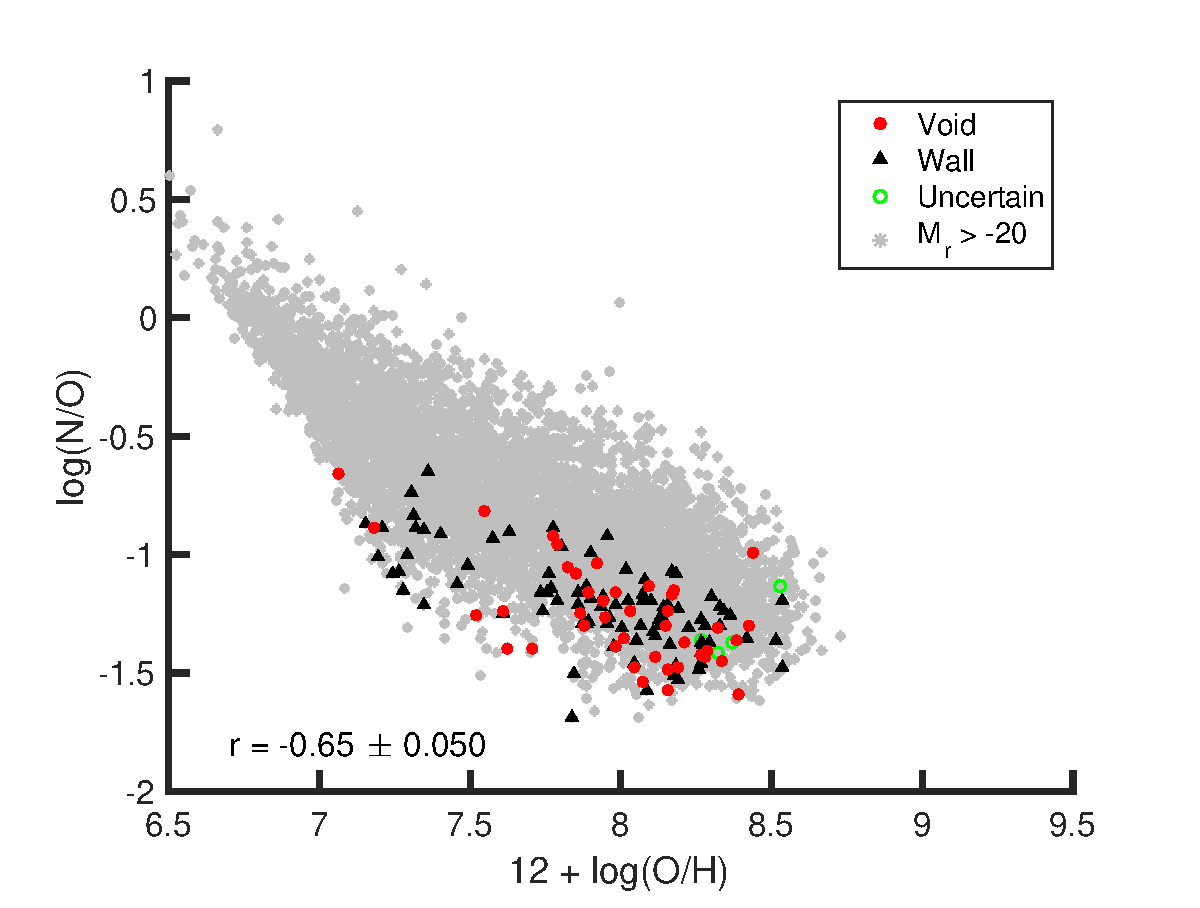
\includegraphics[width=0.5\textwidth]{Images/Paper2/1sig_I06_dwarf_0-20_SF_t3_Z12logOH_logNO}
    \caption[N/O versus metallicity of 135 dwarf galaxy sample]{N/O as a 
    function of O/H for star-forming void (red circles) and wall (black 
    triangles) dwarf galaxies.  Error bars have been omitted for clarity.  N/O 
    is expected to be constant for $12 + \log (\text{O}/\text{H}) \lesssim 8.5$, 
    as the metallicity of a galaxy's ISM is too low for stars to be created with 
    enough of the heavy elements to undergo the CNO cycle early enough in their 
    lifetimes.  As a result, nitrogen behaves as a primary element at galactic 
    metallicities less than approximately 8.5.  To place the dwarf galaxies in 
    the context of the general galaxy population, we also plot (gray stars) all 
    star-forming galaxies fainter than $M_r > -20$.}
    \label{fig:OvN}
\end{figure}

If a plateau in the O/H--N/O relation exists, then we should see a slope of 1 in 
the O/H--N/H relation.  When looking at N/H as a function of O/H in Fig. 
\ref{fig:OHvNH}, we see that there is a correlation between the nitrogen and 
oxygen abundances.  However, a best fit to the dwarf galaxies reveals a slope of 
only $0.62\pm 0.078$ --- the nitrogen abundance increases at a slower rate than 
the oxygen abundance.  This result matches the negative relationship between the 
metallicity and the N/O ratio seen in Fig. \ref{fig:OvN}.  If we examine only 
the low-metallicity ($12 + \log(\text{O}/\text{H}) < 7.6$) star-forming galaxies 
with $M_r > -20$, a linear fit produces a slope of $0.05\pm 0.019$ in Fig. 
\ref{fig:OHvNH} and a slope of $-0.94\pm 0.019$ in Fig. \ref{fig:OvN}.  This is 
in sharp contrast to the star-forming galaxies with $M_r > -20$ that have 
metallicities $12 + \log(\text{O}/\text{H}) > 7.6$, where their slope in Fig. 
\ref{fig:OHvNH} is $0.60\pm 0.022$ and $-0.39\pm 0.023$ in Fig. \ref{fig:OvN}.  
It appears that the nitrogen production is independent of the amount of oxygen 
produced in low-metallicity systems.  At normal metallicities 
($7.6 < 12 + \log(\text{O}/\text{H}) < 8.5$), there exists a positive 
relationship between the production of nitrogen and oxygen, although the ratio 
of N/O produced depends on the galaxy's metallicity.

There is no difference between void and wall galaxies in the relationship of 
oxygen and nitrogen production in the low-metallicity sample.  There is a slight 
difference in slopes between the void and wall galaxies with normal 
metallicities, where the void galaxies have a larger slope in the relationship 
between O/H and N/H and a smaller slope in the relationship between O/H and N/O.  
While statistically significant, the difference in the slopes between the two 
environments is not large enough to be physically relevant.  The significant 
scatter in both Figs. \ref{fig:OHvNH} and \ref{fig:OvN} indicates that the 
described relationships between the production of nitrogen and oxygen are only 
global trends in the nucleosynthesis of the galaxies.

\begin{figure}
    \centering
    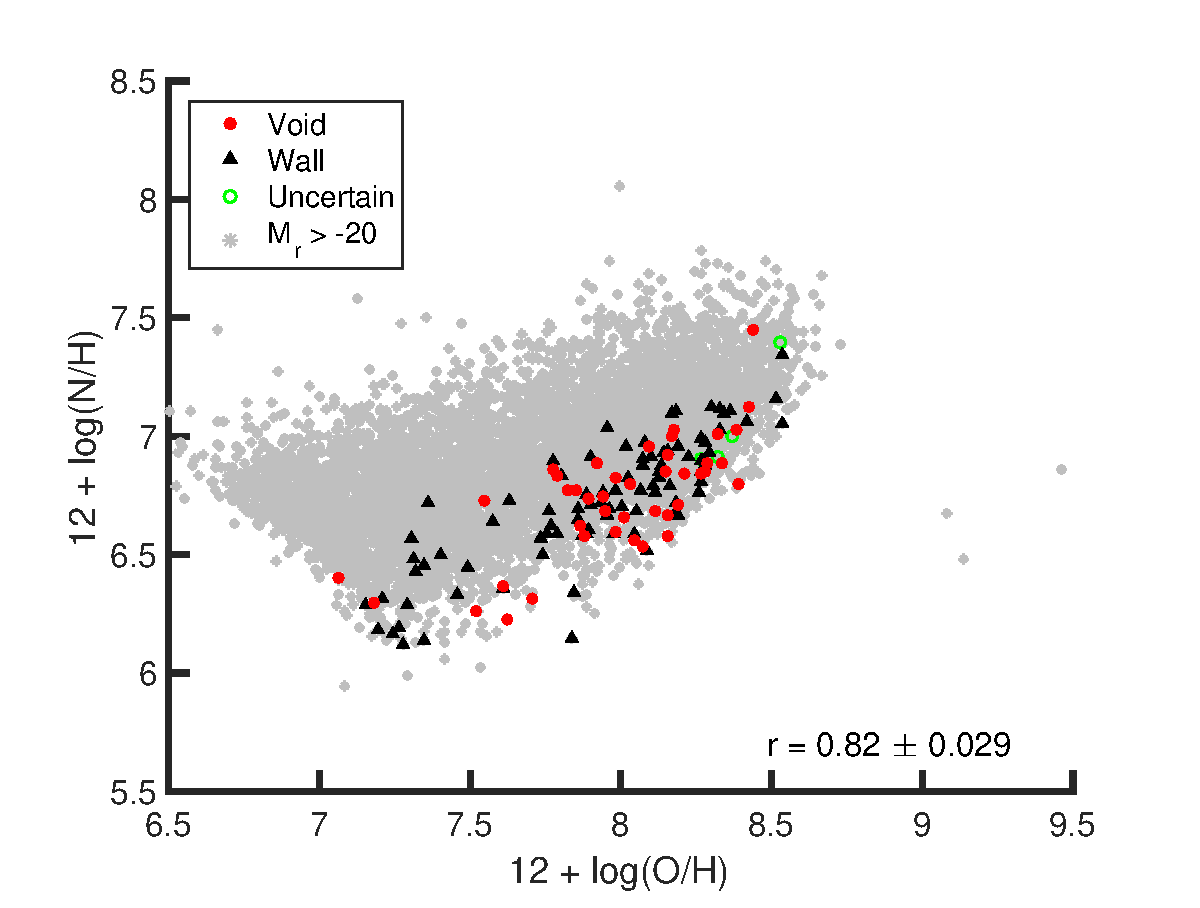
\includegraphics[width=0.5\textwidth]{Images/Paper2/1sig_I06_dwarf_0-20_SF_t3_Z12logOH_N12logNH}
    \caption[N/H versus metallicity for 135 dwarf galaxy sample]{N/H as a 
    function of O/H for star-forming void (red circles) and wall (black 
    triangles) dwarf galaxies.  Error bars have been omitted for clarity.  There 
    is a positive correlation between the two abundances.  With a best-fit slope 
    less than 1, we see that the synthesis of nitrogen in these galaxies is 
    primary.}
    \label{fig:OHvNH}
\end{figure}


%-------------------------------------------------------------------------------
%\subsection{Comparison to previously published abundance estimates}

% Amorin10 does not publish their N/O estimates


%-------------------------------------------------------------------------------
\subsection{Mass--N/O relation}\label{sec:Mass_NO}

Just as there is a well-known mass--metallicity relation for galaxies 
\citep[where the metallicity increases with stellar mass; see, 
e.g.,][]{Tremonti04}, there is also a mass--N/O relation.  We expect to see a 
primary N/O plateau in the mass--N/O relation, since galaxies with lower stellar 
masses have not yet produced enough heavy elements to synthesize more nitrogen 
than oxygen.  Beyond the low-mass limit, there should be a steady increase in 
the N/O ratio as a function of stellar mass, due to secondary nitrogen 
enrichment.  Our dwarf galaxies in Fig. \ref{fig:MNO} show a steady increase in 
N/O as a function of stellar mass; there is a hint of the beginnings of a 
plateau for $\log(M_*/M_{\odot}) \lesssim 8$.  The lack of a plateau here could 
be a result of our limited stellar mass range for the dwarf galaxies.  A linear 
fit to our dwarf galaxies reveals a slope of $0.6\pm 0.12$, which is much 
stronger than the slope of $0.30$ found by \cite{Andrews13}.

% Compare with results from Andrews13, Amorin10, PerezMontero09, PerezMontero13
From Fig. \ref{fig:MNO}, we conclude that the N/O plateau, if one exists, starts 
around $\log(M_*/M_{\odot}) \approx 8$.  This is at a much lower mass than that 
found by \cite{Andrews13} --- they claim the N/O plateau exists for galaxies 
with $\log(M_*/M_{\odot}) < 8.9$.  However, our relationship between stellar 
mass and N/O matches Fig. 3 of \cite{Amorin10}, as well as the results of 
\cite{PerezMontero09} and \cite{PerezMontero13}.  None of our data samples 
display an obvious N/O plateau above a stellar mass 
$\log(M_*/M_{\odot}) > 8$, indicative of primary nitrogen versus secondary 
nitrogen production in galaxies.  This could indicate that the switch from 
primary to secondary nitrogen production occurs at a much lower stellar mass 
than found by \cite{Andrews13}.  More low-mass galaxies are needed to extend 
this relation below $\log(M_*/M_{\odot}) < 8$.

\begin{figure}
    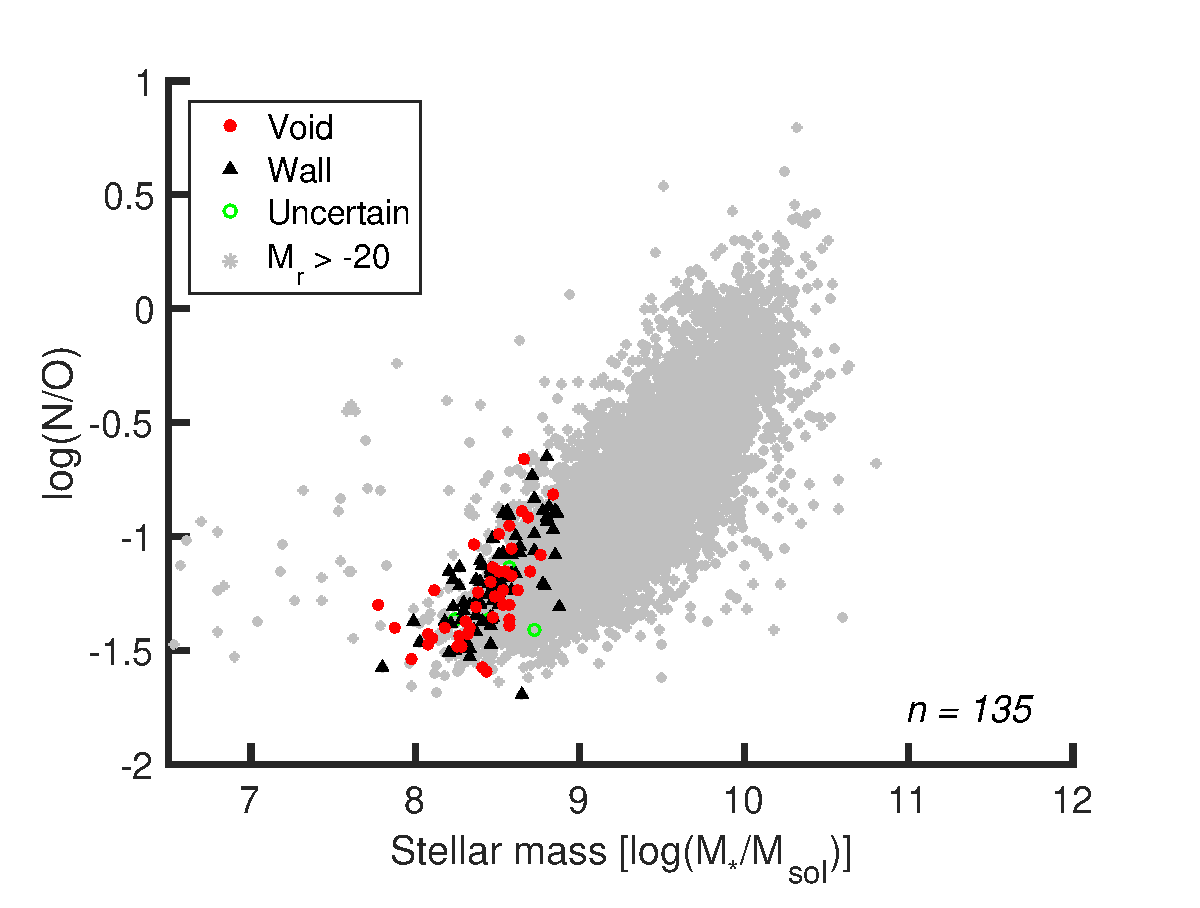
\includegraphics[width=0.5\textwidth]{Images/Paper2/MNO_1sig_I06_dwarf_0-20_SF_t3}
    \caption[Stellar mass versus N/O for 135 dwarf galaxy sample]{Mass--N/O 
    relation for star-forming void (red circles) and wall (black triangles) 
    dwarf galaxies.  Error bars have been omitted for clarity.  N/O is expected 
    to remain constant for low stellar masses and increase steadily for larger 
    masses, due to the mass-metallicity relation and the primary vs. secondary 
    synthesis of nitrogen.  To place the dwarf galaxies in the context of the 
    general galaxy population, we also plot (gray stars) the star-forming 
    galaxies with $M_r > -20$.}
    \label{fig:MNO}
\end{figure}


%-------------------------------------------------------------------------------
\subsection{Color--N/O relation}

% Compare to Fig. 9 of vanZee06a, Fig. 6 of Berg12
As \cite{vanZee06a} and \cite{Berg12} discuss, a time delay between the release 
of nitrogen and oxygen will result in a positive relationship between the N/O 
ratio and the color of a galaxy.  If oxygen is primarily produced in higher-mass 
stars (and since these stars die earlier than the intermediate-mass stars 
responsible for the synthesis of nitrogen), then, for a given star formation 
episode, the oxygen produced will be released on a shorter time scale than the 
nitrogen.  As a result, the amount of nitrogen relative to oxygen should 
increase as the hotter, more massive stars die and the galaxy becomes redder.  
This is exactly what we see in Fig. \ref{fig:color_NO}.  We use rest-frame 
colors $K$-corrected to a redshift of 0.1; they are corrected for galactic 
extinction and calculated with model magnitudes \citep{Choi10}.  
\cite{vanZee06a} and \cite{Berg12} also found an increase in the N/O ratio as a 
function of color.

\begin{figure*}
    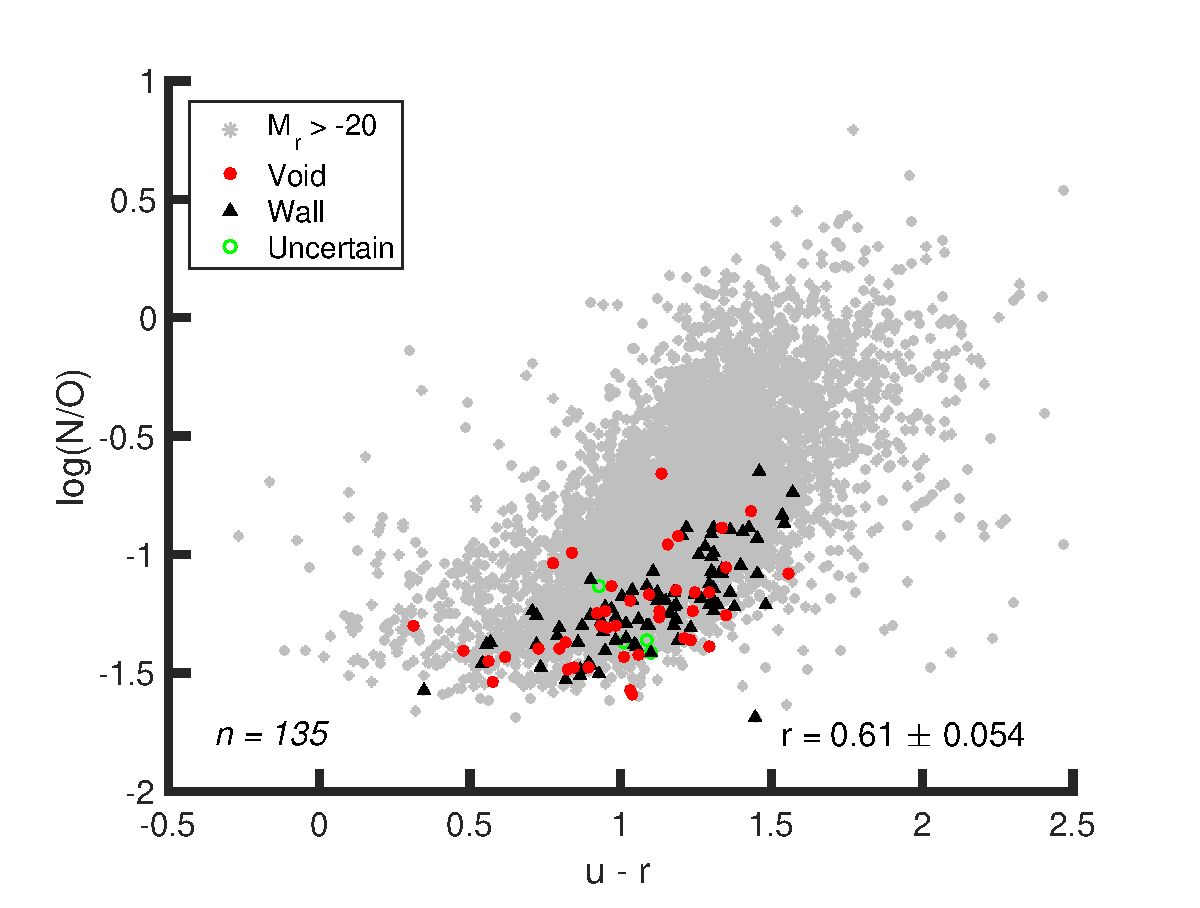
\includegraphics[width=0.49\textwidth]{Images/Paper2/ur_NO_1sig_I06_dwarf_0-20_SF_t3}
    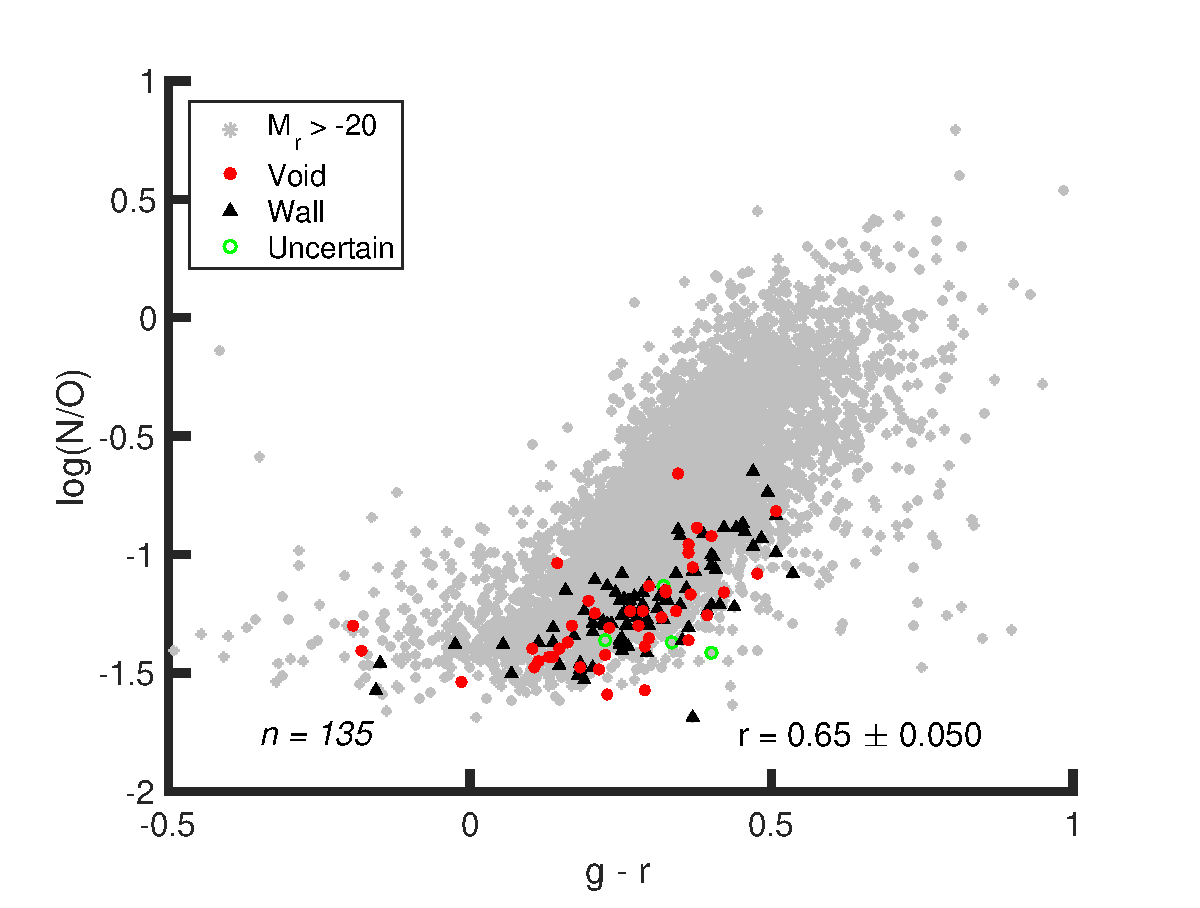
\includegraphics[width=0.49\textwidth]{Images/Paper2/gr_NO_1sig_I06_dwarf_0-20_SF_t3}
    \caption[Color versus N/O for 135 dwarf galaxy sample]{Color ($u-r$ and 
    $g-r$) vs. N/O ratio for star-forming void (red circles) and wall (black 
    triangles) dwarf galaxies.  Error bars have been omitted for clarity.  N/O 
    is expected to increase as galaxies become redder if there is a time delay 
    between the release of oxygen and nitrogen.  To place the dwarf galaxies in 
    context, we also plot the star-forming galaxies with $M_r > -20$ 
    (gray stars).}
    \label{fig:color_NO}
\end{figure*}


%-------------------------------------------------------------------------------
\subsection{(s)SFR--N/O relation}

We expect there to be a correlation between SFR or sSFR (per unit stellar mass) 
and the N/O ratio in galaxies as a result of the positive correlations between 
the SFR and stellar mass of a galaxy \citep{Brinchmann04} and the sSFR and the 
color of a galaxy (Fig. \ref{fig:color_sSFR}).  As shown in Fig. \ref{fig:MNO}, 
the N/O ratio increases with increasing stellar mass.  As a result, we expect 
there to be a positive correlation between the SFR and N/O ratio in our 
galaxies.  This can be seen in the sample of star-forming galaxies with 
$M_r > -20$ in the left panel of Fig. \ref{fig:SFR_NO}.  Due to the large 
scatter in this relation, the blue star-forming dwarf galaxies exhibit a 
negative correlation between their N/O ratios and their SFRs.  These SFR are 
aperture corrected to estimate the total SFR in the galaxy (not just within the 
SDSS fiber).

\begin{figure*}
    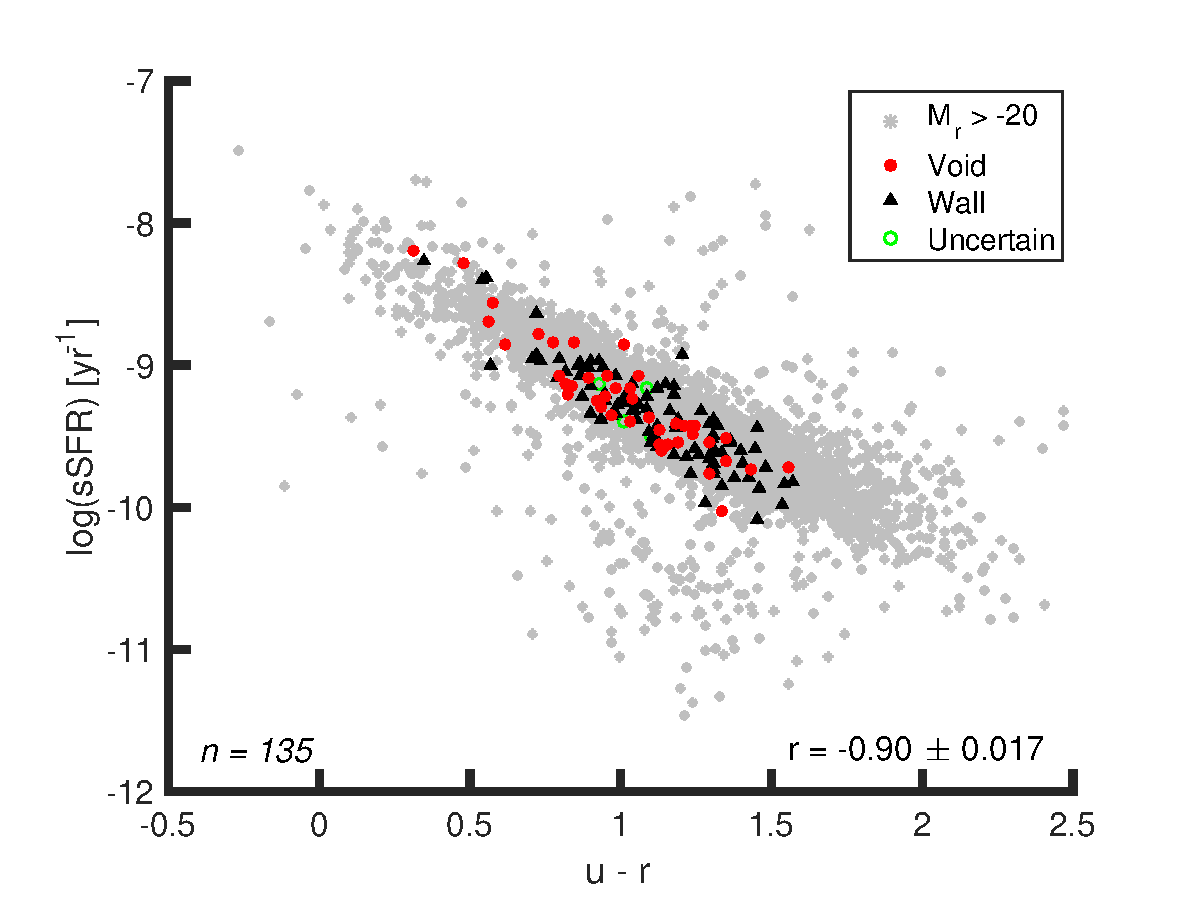
\includegraphics[width=0.49\textwidth]{Images/Paper2/u-r_sSFR_dwarf_0-20_SF_t3}
    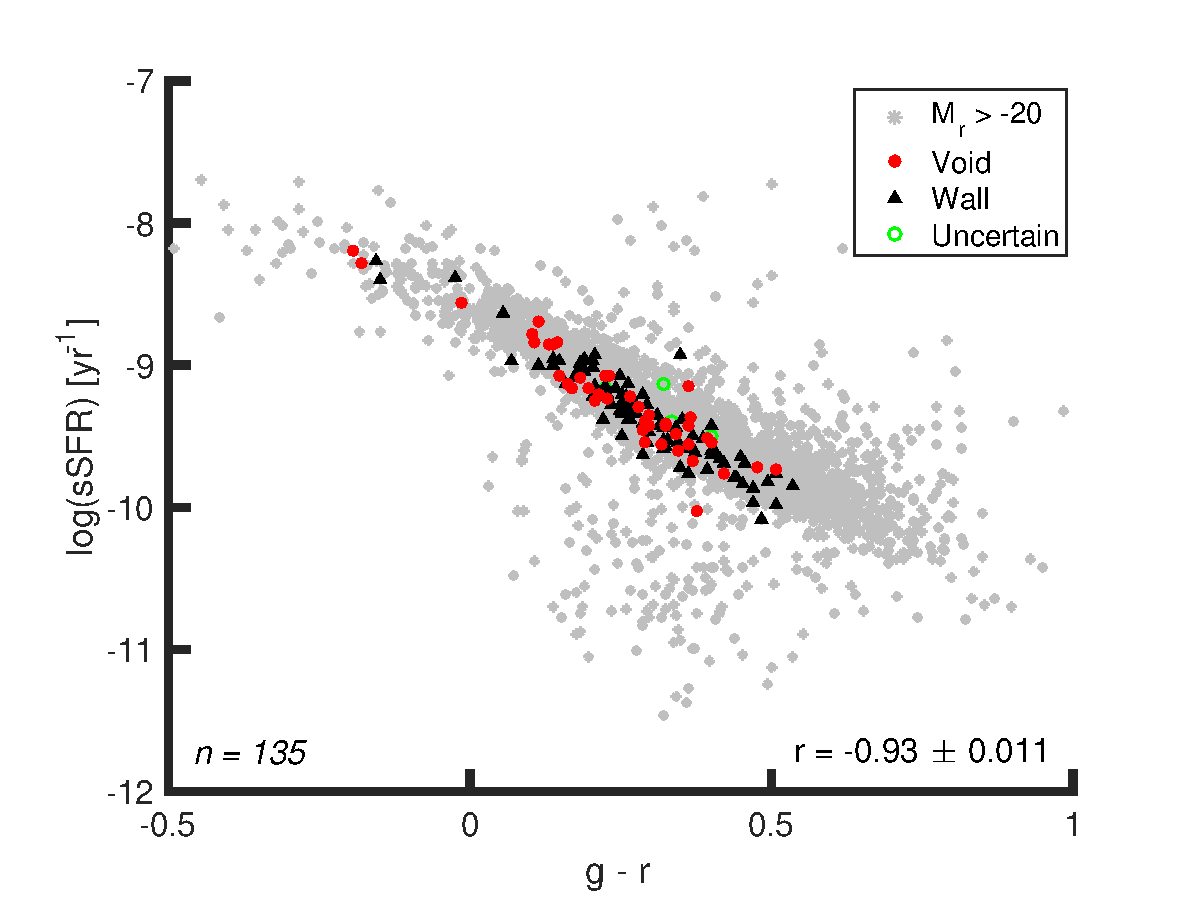
\includegraphics[width=0.49\textwidth]{Images/Paper2/g-r_sSFR_dwarf_0-20_SF_t3}
    \caption[Color versus sSFR for 135 dwarf galaxy sample]{Color ($u-r$ and 
    $g-r$) vs. sSFR for star-forming void (red circles) and wall (black 
    triangles) dwarf galaxies.  It is obvious that there is a negative 
    correlation between the $\log (sSFR)$ and the color of a galaxy.  To place 
    the dwarf galaxies in context, we also show the star-forming galaxies with 
    $M_r > -20$ (gray stars).}
    \label{fig:color_sSFR}
\end{figure*}

The N/O ratio is expected to decrease as sSFR increases in galaxies, as is shown 
in the right panel of Fig. \ref{fig:SFR_NO}.  Bluer galaxies have higher sSFR.  
Fig. \ref{fig:color_NO} shows that there is a positive correlation between the 
color and the N/O ratio, such that bluer galaxies have lower N/O ratios.  As a 
result, we are not surprised to see that the N/O ratio decreases as the sSFR 
increases.
%Oxygen is produced in higher-mass stars 
%than nitrogen.  Since a star's lifetime is inversely proportional to its mass, 
%the stars that produce oxygen will die and release their heavy elements to the 
%ISM sooner than the stars responsible for producing nitrogen.  As a result, 
%after a recent star formation episode (when the sSFR is high), the amount of 
%oxygen will increase relative to nitrogen, decreasing the N/O ratio.  As the 
%sSFR of a galaxy declines, its N/O ratio will slowly increase as the nitrogen in 
%the intermediate-mass stars is released.

\begin{figure*}
    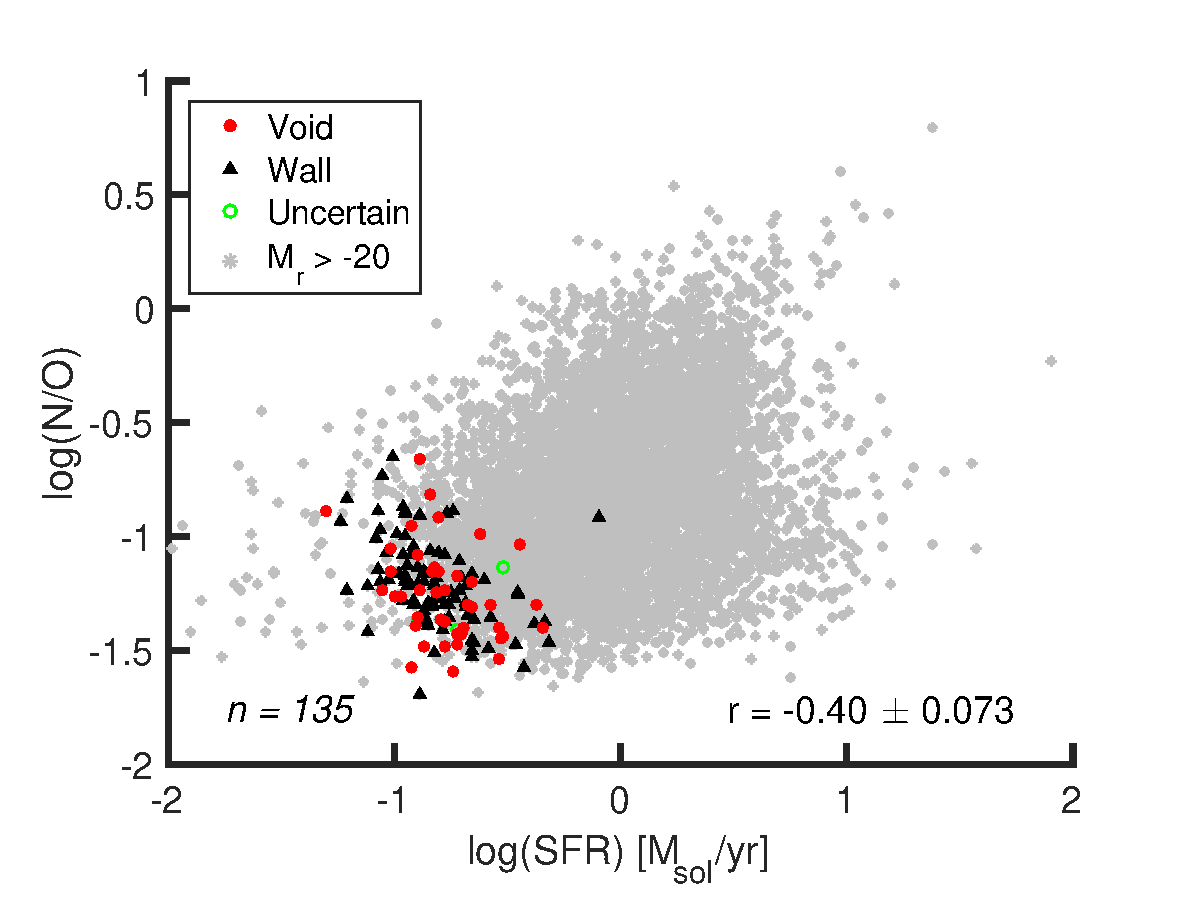
\includegraphics[width=0.49\textwidth]{Images/Paper2/SFR_NO_1sig_I06_dwarf_0-20_SF_t3}
    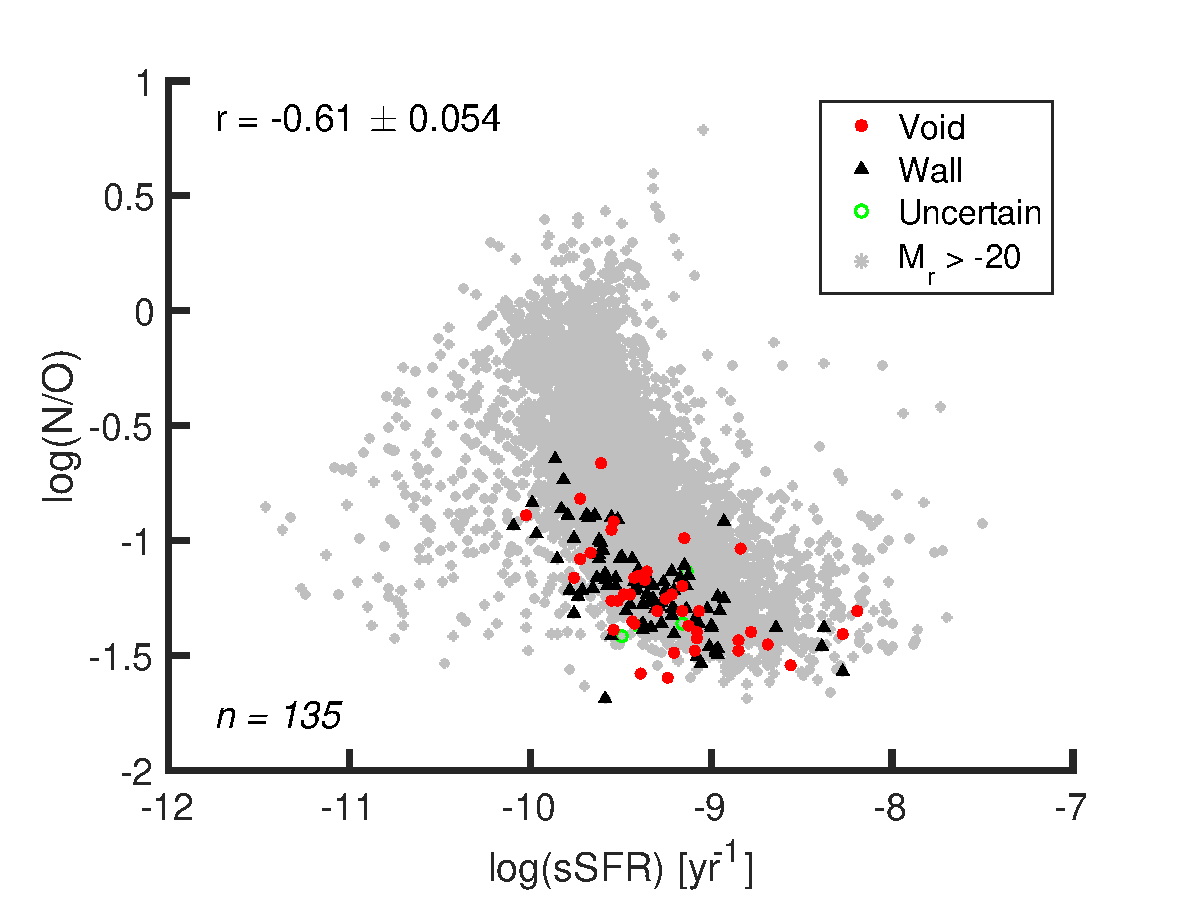
\includegraphics[width=0.49\textwidth]{Images/Paper2/sSFR_NO_1sig_I06_dwarf_0-20_SF_t3}
    \caption[(s)SFR versus N/O for 135 dwarf galaxy sample]{SFR--N/O and 
    sSFR--N/O relations for star-forming void (red circles) and wall (black 
    triangles) dwarf galaxies.  Error bars have been omitted for clarity.  Based 
    on the correlations between SFR and stellar mass and sSFR and color, we 
    expect the N/O ratio to increase with increasing SFR and decrease with sSFR.  
    To place the dwarf galaxies in context, we also show the star-forming 
    galaxies with $M_r > -20$ (gray stars).}
    \label{fig:SFR_NO}
\end{figure*}


%%%%%%%%%%%%%%%%%%%%%%%%%%%%%%%%%%%%%%%%%%%%%%%%%%%%%%%%%%%%%%%%%%%%%%%%%%%%%%%%
%
%    DISCUSSION
%
%%%%%%%%%%%%%%%%%%%%%%%%%%%%%%%%%%%%%%%%%%%%%%%%%%%%%%%%%%%%%%%%%%%%%%%%%%%%%%%%
\section[Discussion]{Large-scale environmental influence}\label{sec:environment}

The majority of the shifts in the gas-phase abundances of oxygen, nitrogen, and 
the N/O ratio seen in galaxies fainter than $L_*$ are small and statistically 
insignificant.  However, they occur in almost the same direction across all 
magnitude bins.  This trend suggests that the gas-phase abundances may be 
influenced by the galaxies' large-scale environments.  \cite{Shields91} find no 
offset in the N/O ratio between cluster and field galaxies, despite the 
difference in O/H they observe.  Similar to us, \cite{Contini02} and 
\cite{Pilyugin02} also find a statistically insignificant shift in the N/O ratio 
of cluster galaxies, although they find that these galaxies have lower N/O 
ratios than field spiral galaxies.  Based on Fig. \ref{fig:NOratio} and the 
statistics in Table \ref{tab:stats}, we find weak evidence that void dwarf 
galaxies have a smaller N/O ratio than dwarf galaxies in denser regions.  This 
means that void dwarf galaxies may have more oxygen than wall dwarf galaxies, 
and/or void dwarf galaxies could have less nitrogen than wall dwarf galaxies.  
Here we discuss these possibilities and explore their implications for the 
large-scale environmental impact on the formation and evolution of galaxies.

%If there was more oxygen in void dwarf galaxies than wall dwarf galaxies, then 
%we would expect to see this reflected in the oxygen abundance distributions.  
%However, as Fig. \ref{fig:met1sig} shows, this is not the case --- both void and 
%wall dwarf galaxies have equal distributions of oxygen abundance.  Therefore, to 
%have a difference in oxygen but to return the results seen in Fig. 
%\ref{fig:met1sig}, void dwarf galaxies must then also have more hydrogen than 
%wall dwarf galaxies.  This is definitely possible, as we expect that void 
%galaxies are more privy to an inflow of pristine hydrogen-rich gas than wall 
%galaxies.  However, explaining the excess oxygen in void galaxies is more 
%difficult.  Void dwarf galaxies might retain more of their metals than do wall 
%dwarf galaxies because of the absence of tidal forces, ram pressure stripping, 
%etc. in the void environment.
%
%On the other hand, the difference in Fig. \ref{fig:NOratio} could also be 
%explained by there being less nitrogen in void dwarf galaxies than wall dwarf 
%galaxies.  This would seem to match the theory more, since it is thought that 
%void galaxies should produce fewer metals.  However, this result is not 
%reflected in Fig. \ref{fig:N_1sig}, since the two populations are centered on 
%similar values of $12 + \log \left( \text{N}/\text{H} \right)$.

Table \ref{tab:stats} suggests a slight large-scale environmental dependence of 
the oxygen and nitrogen abundances (relative to hydrogen), where void galaxies 
have slightly more O/H and N/H than wall galaxies.  This small difference is 
not apparent when looking at Figs. \ref{fig:met1sig} and \ref{fig:N_1sig}.  
However, the N/O ratio amplifies this large-scale environmental effect so that a 
shift in the mean (or median) of the two populations can be seen in Fig. 
\ref{fig:NOratio}.  We hesitate to combine the results across all magnitude bins 
in an effort to improve their significance.  Instead, we look toward the future 
to analyze a larger sample of galaxies to increase the statistical significance 
of these results.

\subsection{Higher metallicities in void dwarf galaxies}

A slightly higher metallicity in void dwarf galaxies than wall dwarf galaxies 
may be evidence of a difference in the ratio of dark matter halo mass to stellar 
mass between the two environments.  Simulations by \cite{Jung14} and 
\cite{Tonnesen15} show that the dark matter halo masses of void central galaxies 
are larger than those of wall central galaxies for a given stellar mass.  Due to 
their environment, void dwarf galaxies are more likely to be in the center of 
their own dark matter halo.  Wall dwarf galaxies, on the other hand, are much 
more likely to be a satellite galaxy within a much larger dark matter halo; the 
simulation results mentioned above would not apply to these wall dwarf galaxies.  
However, because the wall dwarf galaxies studied here have sufficiently high 
sSFRs, they most likely live in a small-scale environment very similar to that 
of the void dwarf galaxies, as discussed in Paper I.  As a result, it is likely 
that (and should be tested to see whether) the wall dwarf galaxies in this study 
are actually central galaxies.  

Applying the results of these simulations to our dwarf galaxy sample, if the 
ratio of dark matter halo mass to stellar mass is larger in void galaxies, the 
metals ejected from a void galaxy's ISM into its circumgalactic medium are more 
likely to fall back onto the ISM than in a wall galaxy with the same stellar 
mass, since the void galaxy's virial radius and potential well are larger.  As a 
result, two dwarf galaxies with the same stellar mass in these two different 
large-scale environments can have different metallicities --- void dwarf 
galaxies would have higher metallicities than wall dwarf galaxies, matching what 
we see in Table \ref{tab:stats}.

\subsection{Lower N/O ratios in void dwarf galaxies}

A difference in the N/O ratio between void dwarf galaxies and wall dwarf 
galaxies could be a result of the difference in the synthesis of nitrogen in 
galaxies within these two large-scale environments.  If void galaxies are 
retarded in their star formation (as simulations of the $\Lambda$CDM cosmology 
suggest), then cosmic downsizing would reduce the SFR at late times much more in 
wall galaxies than in void galaxies.  As a result, the minimum gas-phase 
metallicity required for the production of secondary nitrogen in walls would be 
achieved at an earlier time in the galaxy's lifetime than in a void galaxy.  
This would cause the N/O ratio in wall galaxies to be larger than that in voids.  
\cite{vanZee06a} suggest that a galaxy with a declining SFR (wall galaxies) will 
have a higher nitrogen-to-oxygen yield than a galaxy with a constant SFR (void 
galaxies).  This is due to more oxygen being released into the ISM as a result 
of the ongoing star formation in the void galaxies.  This explanation is 
supported by the color--N/O diagram in Fig. \ref{fig:color_NO}, which reveals 
that redder galaxies have higher N/O ratios.  The correlation between color and 
the N/O ratio found in \cite{vanZee06a}, \cite{Berg12}, and Fig. 
\ref{fig:color_NO} is a result of declining SFRs \citep{vanZee06a}.  Therefore, 
the shift in the N/O ratio we see between void and wall galaxies may be 
observational evidence of retarded star formation in void galaxies as a result 
of cosmic downsizing.
%If wall galaxies have a higher 
%N/H ratio than void galaxies, they could be producing nitrogen as a secondary 
%element more so than void dwarf galaxies.  This would cause the N/O ratio in 
%wall galaxies to be larger than that in voids.

Another explanation that would lead to a shift in the N/O ratio between 
environments is a difference in the ratio of intermediate- and high-mass stars 
produced in void and wall dwarf galaxies.  For there to be more oxygen relative 
to nitrogen in void dwarf galaxies, the percent of higher-mass stars produced in 
a star formation episode would be higher than that in wall dwarf galaxies.  This 
would indicate a varying IMF as a function of large-scale environment.  Previous 
studies have been inconclusive when testing for a varying IMF \citep[see][for 
example]{Kroupa01, Kroupa02, Hoversten08, Meurer09}.  It is beyond the scope of 
this paper to elaborate on this explanation.
%This is the opposite of the (extremely mild) offset between the two environments 
%that Ginny found.


%-------------------------------------------------------------------------------
\subsection{N/O ratio for extremely low metallicity galaxies}

While Paper I shows that there is not a special population of extremely low 
metallicity dwarf galaxies residing in voids, we want to look in particular at 
the N/O ratio of extremely low metallicity galaxies.  For the 21 dwarf galaxies 
with $12 + \log (\text{O}/\text{H}) < 7.6$ identified in Paper I, we see from 
Fig. \ref{fig:OHvNH} that their N/H ratios are also some of the lowest in the 
dwarf galaxy sample.  However, as shown in Fig. \ref{fig:OvN}, their N/O ratios 
cover the range of N/O ratio values of all the dwarf galaxies studied.  This is 
consistent with the expectation that nitrogen behaves as a primary element for 
galaxies with low and moderate metallicities.  Details of these 21 dwarf 
galaxies with extremely low metallicities are listed in Table \ref{tab:lowZ_P2}, 
including their gas-phase chemical abundances.

\begin{sidewaystable}
\centering

\begin{tabular}{ccccccccccc}
Index\footnote{KIAS-VAGC galaxy index number} & R.A. & Decl. & Redshift & \multicolumn{2}{c}{$12 + \log \left( \frac{\text{O}}{\text{H}} \right)$} & \multicolumn{2}{c}{$12 + \log \left( \frac{\text{N}}{\text{H}} \right)$} & \multicolumn{2}{c}{$\log \left( \frac{\text{N}}{\text{O}} \right)$} & Void/Wall \\
\hline \\
268470 & \RA{13}{18}{17}{.82} & +\dec{02}{12}{59}{.83} & 0.0252 & 7.06 & $\pm$0.37 & 6.40 & $\pm$0.25 & -0.66 & $\pm$0.45 & Void \\
1422637 & \RA{14}{18}{12}{.14} & +\dec{13}{59}{33}{.98} & 0.0261 & 7.15 & $\pm$0.41 & 6.29 & $\pm$0.28 & -0.87 & $\pm$0.50 & Wall \\
839665 & \RA{08}{09}{53}{.53} & +\dec{29}{17}{04}{.82} & 0.0281 & 7.18 & $\pm$0.44 & 6.29 & $\pm$0.31 & -0.89 & $\pm$0.54 & Void \\
1168448 & \RA{11}{06}{41}{.00} & +\dec{45}{19}{09}{.28} & 0.0220 & 7.19 & $\pm$0.46 & 6.18 & $\pm$0.32 & -1.01 & $\pm$0.57 & Wall \\
1299291 & \RA{12}{17}{14}{.02} & +\dec{43}{18}{53}{.36} & 0.0233 & 7.21 & $\pm$0.42 & 6.32 & $\pm$0.29 & -0.89 & $\pm$0.51 & Wall \\
1170573 & \RA{11}{05}{39}{.42} & +\dec{46}{03}{28}{.37} & 0.0250 & 7.24 & $\pm$0.34 & 6.16 & $\pm$0.23 & -1.08 & $\pm$0.41 & Wall \\
2288717 & \RA{10}{46}{12}{.18} & +\dec{21}{31}{37}{.37} & 0.0248 & 7.27 & $\pm$0.48 & 6.19 & $\pm$0.33 & -1.08 & $\pm$0.58 & Wall \\
955643 & \RA{11}{42}{03}{.02} & +\dec{49}{21}{25}{.18} & 0.0244 & 7.28 & $\pm$0.44 & 6.12 & $\pm$0.30 & -1.15 & $\pm$0.53 & Wall \\
1344311 & \RA{12}{33}{13}{.64} & +\dec{11}{10}{28}{.46} & 0.0245 & 7.29 & $\pm$0.50 & 6.29 & $\pm$0.34 & -1.00 & $\pm$0.61 & Wall \\
1254352 & \RA{13}{29}{02}{.45} & +\dec{10}{54}{55}{.80} & 0.0237 & 7.30 & $\pm$0.44 & 6.57 & $\pm$0.30 & -0.73 & $\pm$0.54 & Wall \\
1857820 & \RA{08}{45}{00}{.34} & +\dec{27}{16}{47}{.04} & 0.0257 & 7.31 & $\pm$0.48 & 6.48 & $\pm$0.33 & -0.83 & $\pm$0.59 & Wall \\
866876 & \RA{09}{04}{57}{.96} & +\dec{41}{29}{36}{.42} & 0.0240 & 7.32 & $\pm$0.40 & 6.43 & $\pm$0.28 & -0.89 & $\pm$0.49 & Wall \\
833588 & \RA{08}{43}{10}{.71} & +\dec{43}{08}{53}{.58} & 0.0245 & 7.34 & $\pm$0.41 & 6.14 & $\pm$0.29 & -1.21 & $\pm$0.50 & Wall \\
283263 & \RA{14}{14}{12}{.88} & +\dec{01}{50}{12}{.88} & 0.0255 & 7.35 & $\pm$0.43 & 6.45 & $\pm$0.29 & -0.90 & $\pm$0.52 & Wall \\
184308 & \RA{09}{39}{09}{.38} & +\dec{00}{59}{04}{.15} & 0.0244 & 7.36 & $\pm$0.43 & 6.71 & $\pm$0.31 & -0.65 & $\pm$0.53 & Wall \\
1389829 & \RA{14}{31}{01}{.38} & +\dec{38}{04}{21}{.50} & 0.0269 & 7.41 & $\pm$0.46 & 6.50 & $\pm$0.32 & -0.91 & $\pm$0.56 & Wall \\
858951 & \RA{09}{31}{39}{.60} & +\dec{49}{49}{56}{.85} & 0.0251 & 7.46 & $\pm$0.46 & 6.33 & $\pm$0.32 & -1.13 & $\pm$0.57 & Wall \\
1270221 & \RA{13}{27}{39}{.85} & +\dec{50}{54}{09}{.69} & 0.0295 & 7.49 & $\pm$0.43 & 6.45 & $\pm$0.30 & -1.04 & $\pm$0.52 & Wall \\
431383 & \RA{08}{58}{44}{.96} & +\dec{50}{29}{58}{.98} & 0.0230 & 7.52 & $\pm$0.60 & 6.26 & $\pm$0.31 & -1.26 & $\pm$0.68 & Void \\
75442 & \RA{13}{13}{24}{.25} & +\dec{00}{15}{02}{.95} & 0.0264 & 7.55 & $\pm$0.35 & 6.73 & $\pm$0.24 & -0.82 & $\pm$0.42 & Void \\
1322765 & \RA{14}{15}{05}{.58} & +\dec{36}{22}{57}{.77} & 0.0273 & 7.57 & $\pm$0.40 & 6.64 & $\pm$0.28 & -0.93 & $\pm$0.48 & Wall\\
\end{tabular}

\caption[Chemical abundances of extremely low-metallicity dwarf galaxies in 135 galaxy sample]{Details of 21 extremely low gas-phase metallicity ($12 + \log(\text{O}/\text{H}) < 7.6$) galaxies identified in Paper I.  While the N/H values for all these galaxies are also extremely low, the N/O ratios span the range covered by the remainder of the dwarf galaxy sample studied.  Further study of these galaxies is recommended to confirm the abundance values and identify any shared characteristics.}

\label{tab:lowZ_P2}

\end{sidewaystable}



%%%%%%%%%%%%%%%%%%%%%%%%%%%%%%%%%%%%%%%%%%%%%%%%%%%%%%%%%%%%%%%%%%%%%%%%%%%%%%%%
%
%    CONCLUSION
%
%%%%%%%%%%%%%%%%%%%%%%%%%%%%%%%%%%%%%%%%%%%%%%%%%%%%%%%%%%%%%%%%%%%%%%%%%%%%%%%%
\section{Conclusions}

The nucleosynthesis of nitrogen is a vital component of the chemical evolution 
of galaxies in our universe.  We estimate the nitrogen abundance and N/O ratio 
of dwarf galaxies using the direct $T_e$ method and spectroscopic line flux 
measurements from the SDSS DR7 sample as reprocessed in the MPA-JHU catalog.  
The 135 galaxies analyzed suggest a slight large-scale environmental dependence 
of the N/O ratio, where void dwarf galaxies could have a lower N/O ratio than 
dwarf galaxies in denser environments.  Thus, the large-scale 
($\sim 10\text{ Mpc}$) environment might influence the chemical evolution of 
dwarf galaxies.

We find small, statistically insignificant shifts in the mean (or median) N/O 
ratio for galaxies between the void and denser regions across all blue, 
star-forming galaxies with $M_r > -20$.  These shifts are somewhat more 
significant, however, when we look at the entire sample of galaxies.  Each 
magnitude bin is shifted in the same direction, and are potentially very 
interesting, as they might indicate delayed star formation histories, more 
constant SFRs, and larger ratios of dark-matter-halo-mass to stellar mass in 
void galaxies, as discussed in Section \ref{sec:environment}.  A larger sample 
would help test these results.  We look to increase the sample and probe a 
larger magnitude (and mass) range of dwarf galaxies in Douglass \& Vogeley 
(2017, in preparation).

In addition, we look at the relationship between the N/O ratio and other 
physical characteristics of our dwarf galaxies.  In the relation between N/O and 
O/H, our galaxies all reside on the so-called ``nitrogen plateau,'' where the 
N/O ratio is predicted to be constant for low and intermediate metallicities.  
However, instead of a constant value for these galaxies, we find a negative 
correlation between the N/O and O/H ratios.  Our dwarf galaxies show a positive 
correlation between stellar mass and the N/O ratio.  These dwarf galaxies have 
some of the lowest N/O ratios for both their color and (s)SFR.  Beyond the 
suggestive large-scale environmental dependence of the N/O ratio, there is no 
clear large-scale environmental dependence in any of these relationships.

The N/O ratios of the extremely metal-poor dwarf galaxies are no different than 
those of the remaining dwarf galaxy sample, though their N/H abundance is also 
extremely low.  A more detailed study of these 21 extremely metal-poor dwarf 
galaxies is recommended to confirm their abundance values and discover any 
characteristics shared by the population.

Although SDSS provides spectroscopic observations for over 800,000 galaxies, 
only 135 are dwarf galaxies with emission-line fluxes necessary to estimate the 
gas-phase chemical abundances using the direct $T_e$ method.  The greatest 
limiting factor in this sample is the requirement of the [\ion{O}{2}] 
$\lambda 3727$ doublet in the abundance calculations.  We seek to develop a 
work-around for this emission line in Douglass \& Vogeley (2017, in preparation) 
to greatly increase our sample of dwarf galaxies with abundance estimates.  
These estimated ionic abundances can then be compared with environmental 
dependence of star formation and abundance predictions from high-resolution 
hydrodynamic simulations.

Further tests may refine our understanding of the environmental scale that is 
important for determining the chemical evolution of dwarf galaxies.  In 
particular, it will be important to examine whether the influence of relatively 
small-scale ($\sim$2 Mpc) environments is more significant to a dwarf galaxy's 
chemical evolution than the larger-scale environment investigated here.  In 
previous work, both \cite{Kreckel15} and \cite{Beygu17} find little evidence to 
support a significant large-scale environmental influence on the gas content, 
chemical content, or SFR of void galaxies.  Future work will expand on these 
studies with a larger sample and the possible influence they might have on the 
dwarf galaxies' chemical contents and SFRs.  \cite{Beygu17} also investigate any 
connection between a galaxy's physical properties and its location within a 
void.  We also look to study this possible connection with the increased sample 
size of dwarf galaxies in Douglass \& Vogeley (2017, in preparation).

% Chapter: Paper #3 (chemical abundances w/ relationship)
\chapter[O$^+$ Approximation]{Large-Scale Environmental Dependence of Chemical Abundances in Dwarf Galaxies and Implications for Connecting Star Formation and Halo Mass}\label{ch:Paper3}


This chapter has been submitted to the \emph{Astrophysical Journal} by Kelly A. 
Douglass, Michael S. Vogeley, and Renyue Cen; it will be referenced as Douglass 
et. al (2017, submitted).



%%%%%%%%%%%%%%%%%%%%%%%%%%%%%%%%%%%%%%%%%%%%%%%%%%%%%%%%%%%%%%%%%%%%%%%%%%%%%%%%
%
%    ABSTRACT
%
%%%%%%%%%%%%%%%%%%%%%%%%%%%%%%%%%%%%%%%%%%%%%%%%%%%%%%%%%%%%%%%%%%%%%%%%%%%%%%%%
\begin{chapabstract}
We study how the void environment affects the chemical evolution of galaxies in 
the universe by comparing the oxygen and nitrogen abundances of dwarf galaxies 
in voids with dwarf galaxies in denser regions.  Using spectroscopic 
observations from the Sloan Digital Sky Survey Data Release 7, we estimate the 
oxygen and nitrogen abundances of 993 void dwarf galaxies and 759 dwarf galaxies 
in denser regions.  We use the Direct $T_e$ method for calculating the gas-phase 
chemical abundances in the dwarf galaxies because it is best suited for low 
metallicity, low mass (dwarf) galaxies.  A substitute for the [\ion{O}{2}] 
$\lambda 3727$ doublet is developed, permitting oxygen abundance estimates of 
SDSS dwarf galaxies at all redshifts with the Direct $T_e$ method.  We find that 
void dwarf galaxies have slightly higher oxygen abundances ($\sim$7\%) than 
dwarf galaxies in denser environments.  The opposite trend is seen in both the 
nitrogen abundance and N/O ratio: void dwarf galaxies have slightly lower 
nitrogen abundances ($\sim$10\%) and lower N/O ratios ($\sim$17\%) than dwarf 
galaxies in denser regions.  Our mass-N/O relationship shows that the secondary 
production of nitrogen commences at a lower stellar mass in void dwarf 
star-forming galaxies than in dwarf star-forming galaxies in denser 
environments.  We also find that star-forming void dwarf galaxies have higher 
\ion{H}{1} masses than the star-forming dwarf galaxies in denser regions.  Our 
star-forming dwarf galaxy sample demonstrates a strong anti-correlation between 
the sSFR and N/O ratio, providing evidence that oxygen is produced in higher 
mass stars than those which synthesize nitrogen.  The lower N/O ratios and 
smaller stellar mass for secondary nitrogen production seen in void dwarf 
galaxies may indicate both delayed star formation as predicted by $\Lambda$CDM 
cosmology and a dependence of cosmic downsizing on the large-scale environment.  
The shift toward higher oxygen abundances and higher \ion{H}{1} masses in void 
dwarf galaxies might be evidence of larger ratios of dark matter halo mass to 
stellar mass in voids than in denser regions.
\end{chapabstract}


%%%%%%%%%%%%%%%%%%%%%%%%%%%%%%%%%%%%%%%%%%%%%%%%%%%%%%%%%%%%%%%%%%%%%%%%%%%%%%%%
%
%    INTRODUCTION
%
%%%%%%%%%%%%%%%%%%%%%%%%%%%%%%%%%%%%%%%%%%%%%%%%%%%%%%%%%%%%%%%%%%%%%%%%%%%%%%%%
\section{Introduction}


% Primary v. secondary production of nitrogen (reminder) & its influence on the CNO cycle
%% What would cause less nitrogen to be produced in void galaxies?
%Lower production rates of nitrogen relative to oxygen production in void dwarf 
%galaxies could be a consequence of the retarded star formation predicted for 
%dwarf galaxies in voids by the $\Lambda$CDM cosmology.  In stellar 
%nucleosynthesis, there are two main classes of elements: primary and secondary.  
%Primary elements are those produced which do not depend on the quantity of any 
%other elements present in the star (excepting hydrogen, of course).  On the 
%other hand, secondary elements can be synthesized only when other elements are 
%already present in the star at the time of its birth.  Oxygen is a primary 
%element in stellar nucleosynthesis.  There is evidence 
%\textcolor{red}{(SOURCES)} to suggest that nitrogen behaves as both a primary 
%and secondary element.  The main source of nitrogen production is during the CNO 
%cycle, where carbon is needed as a catalyst for the reactions to begin.  If a 
%star is born with enough carbon, then it commences the CNO cycle much earlier 
%than in a star created with only hydrogen (or with only trace amounts of 
%carbon).  If star formation is retarded in void dwarf galaxies, then there are 
%fewer of the heavy elements that have been produced up to this point in time.  
%As a result, the stars that are created have less carbon initially present in 
%the star than in stars within wall dwarf galaxies, and less nitrogen will be 
%produced.  Fig. \ref{fig:N_1sig} shows evidence of this fact --- there is 
%slightly less nitrogen in void dwarf galaxies than in the dwarf galaxies in more 
%dense environments.  


% Prominence of voids in large-scale structure 
% (refs up through Pan et al., other recent void catalogs, ref to van Weygaert review)
Galactic redshift surveys have revealed that the large-scale distribution of 
galaxies is similar to a three-dimensional cosmic web \citep{Bond96}, with thin 
filaments of galaxies connecting galaxy clusters separated by voids (large, 
underdense areas which fill more than 60\% of space).  The voids first 
identified in early surveys \citep[e.g.,][]{Gregory78,Kirshner81,deLapparent86} 
have proven to be a universal feature of large-scale structure.  Analyses of the 
Sloan Digital Sky Survey \citep{Abazajian09,Ahn12} have produced catalogs of 
$10^3$ voids \citep{Pan12,Sutter14}.  Cosmic voids are an essential component for 
understanding the role of a galaxy's environment on its formation and evolution 
\citep[see][for a review]{vandeWeygaert11}.  

% Influence of the large-scale environment on galaxy properties
%  - well-established morphology-density relation (refs starting with Dressler 1980; Postman & Geller 1984)
%  - morphology-luminosity-density (Park et al. 2005?)
%  - evidence that trend continues into voids, where galaxies are found to be bluer, later type, higher sSFR (Rojas et al. 2004, 2005, who attribute this to availability of cool gas to feed star formation, and other refs)
%  - shift of void galaxy luminosity function (Hoyle et al.; Moorman et al.)
%  - consistent with shift of dark matter halo mass function (Goldberg et al.)
%  - investigations of HI properties of void galaxies (Kreckel et al., Moorman et al.)
%  - other refs to "Void galaxy survey" by Kreckel, van de Weygaert et al.
Extensive studies have been performed to understand the role of the environment 
in galaxy formation.  A strong relationship was found between a galaxy's 
morphology and the local density \citep{Dressler80,Postman84}, where the 
fraction of early-type galaxies increases with density.  A galaxy's luminosity 
was found to also contribute to this morphology-luminosity-density relation 
\citep{Park07}.  While much of this early work focused on trends of galaxy 
properties in the densest regions of space, evidence was found that the same 
trends persist into the voids, where galaxies are found to be bluer 
\citep{Grogin99,Rojas04,Patiri06,vonBendaBeckmann08,Hoyle12}, of a later 
morphological type \citep{Grogin00,Rojas04,Park07}, and have higher specific 
star formation rates \citep[sSFR;][]{Rojas05,vonBendaBeckmann08,Moorman15,
Beygu16}.  These trends are attributed to the availability of cool gas to feed 
star formation in the void regions.  \cite{Hoyle05} and \cite{Moorman15} showed 
that there is a shift toward fainter objects in the void galaxy luminosity 
function.  This shift is consistent with the predicted shift of the dark matter 
halo mass function \citep{Goldberg05}.  Investigations into the \ion{H}{1} 
properties of void galaxies have also been performed \citep{Kreckel12,
Moorman14}, where void galaxies tend to have lower \ion{H}{1} masses than 
galaxies in denser environments.  All these observations are consistent with 
predictions from the $\Lambda$CDM cosmology that void galaxies have lower masses 
and be retarded in their star formation when compared to those in denser 
environments \citep[e.g.,][]{Gottlober03,Goldberg05,Cen11}.

% If sSFR are different, and evolutionary history different, is chemical evolution different?
% Suggestions from previous work (Pustilnik et al, others) of very low metallicity in void galaxies
Given that the sSFR and evolutionary history are different for galaxies in 
voids, it follows that their chemical evolution might also be influenced by the 
environment.  The metallicity of a galaxy (a measure of the integrated star 
formation history) is an estimate of the percentage of the galaxy's gas that has 
been processed in stars \citep{Guseva09}.  We would expect void galaxies to have 
lower metallicities than those in denser regions if they have only recently 
commenced forming stars or have recently accreted unprocessed gas.  Observations 
by \cite{Cooper08,Deng11,Filho15,Pustilnik06,Pustilnik11a,Pustilnik11b,
Pustilnik13,Pustilnik14}, and \cite{Pilyugin17} support the hypothesis that void 
galaxies have lower metallicities than galaxies in denser regions.  However, 
\cite{Kreckel15} and \cite{Douglass17a} find no influence from the large-scale 
environment on the metallicity, and \cite{Douglass17b} find that void dwarf 
galaxies have higher metallicities than dwarf galaxies in denser regions.  It is 
obvious that a study of a statistically significant large sample of galaxies is 
required to understand how the large-scale environment influences the chemical 
evolution of galaxies.

% Forcus on dwarf galaxies, which are most sensitive to effects of environment
% SDSS allows void catalog (Pan et al.) and identification of statistically-significant samples of dwarf galaxies (Mr > -17) in voids
% Discuss importance of careful use of metallicity (O/H) estimators - commonly used methods not calibrated for low mass galaxies, so we carefully used "direct" method
% Summary of results in Douglass & Vogeley 2017a,b
Environmental effects should be the most obvious on dwarf galaxies, since they 
possess small gravitational potential wells.  As a result, they are more 
sensitive to astrophysical effects such as cosmological reionization, internal 
feedback from supernova and photoheating from star formation, external effects 
from tidal interactions and ram pressure stripping, small-scale details of dark 
matter halo assembly, and properties of dark matter.  The main galaxy sample of 
SDSS DR7 covers a large enough volume to identify over 1000 voids \citep{Pan12} 
along with a statistically-significant sample of dwarf galaxies ($M_r > -17$) in 
voids.  SDSS also provides spectroscopy that permits metallicity estimates of 
this large sample of dwarf galaxies.

Numerous methods to estimate the metallicity of an object have been developed 
over the years, as a result of the availability of various spectral features.  
All methods except the direct $T_e$ method are calibrated on galaxies with 
various characteristics, making it unwise to apply them to galaxies outside the 
groups from which these calibrations were derived.  The commonly used methods 
are not calibrated for low-mass galaxies, so we carefully chose to use the 
Direct $T_e$ method because we are focusing on only dwarf galaxies.  A detailed 
explanation of this and other method classes can be found in \cite{Douglass17a}.  
With this estimator, \cite{Douglass17a} and \cite{Douglass17b} have looked at 
the gas-phase chemical abundances of 135 star-forming dwarf galaxies.  They 
found that the large-scale environment has very little influence on the oxygen 
and nitrogen abundances in star-forming dwarf galaxies.  However, their sample 
does indicate that star-forming void galaxies have lower N/O ratios than 
star-forming dwarf galaxies in denser regions.  This is attributed to delayed 
star formation in void galaxies, along with a possible environmental influence 
on cosmic downsizing.  They also argue that the very slight shift towards higher 
oxygen abundances in star-forming void dwarf galaxies could be due to a larger 
ratio of dark matter halo mass to stellar mass in void dwarf galaxies.

% In this paper...
% New approach to O abundance estimation - allows use of larger sample.  Still using "direct" method.
% Note that this work examines dwarf, star-forming galaxies only
% Here we also examine HI properties
% Known influence of environment on morphology already taken into account (well, not exactly because we select on emission lines, not morphology from photometry) - we look only at star-forming galaxies
% Known influence of environment on luminosity already taken into account - we look only at dwarfs
We look to expand on the work by \cite{Douglass17a,Douglass17b} by substantially 
increasing their sample size of dwarf galaxies.  The main limiting factor in 
their sample was due to the required detection of the [\ion{O}{2}] $\lambda$3727 
doublet, which is needed to estimate the amount of singly-ionized oxygen 
present.  We present a new approach to the O$^+$ abundance estimation, which 
removes the need for this emission line.  This calculation is used in 
conjunction with the Direct $T_e$ method to estimate the total gas-phase oxygen 
abundance in galaxies.  We also examine the relationship between the chemical 
abundance and \ion{H}{1} mass of star-forming dwarf galaxies.  For reasons 
described above, this work only examines the chemical evolution of star-forming 
dwarf galaxies.  As a result of this sample, the known influences of the 
environment on the morphology and luminosity have already be taken into account, 
since we concentrate only on star-forming dwarf galaxies.

% THEORY
% Discuss above as motivation or save for Discussion? - save for discusson (KAD)
% Ref Cen simulation paper that shows that void have cool gas available for star formation
% Ref Tonnesen & Cen simulation paper


%%%%%%%%%%%%%%%%%%%%%%%%%%%%%%%%%%%%%%%%%%%%%%%%%%%%%%%%%%%%%%%%%%%%%%%%%%%%%%%%
%
%    THEORY
%
%%%%%%%%%%%%%%%%%%%%%%%%%%%%%%%%%%%%%%%%%%%%%%%%%%%%%%%%%%%%%%%%%%%%%%%%%%%%%%%%
\section[Abundance calculations]{Estimation of gas-phase chemical abundances from optical spectroscopy}

We study a galaxy's oxygen and nitrogen abundances for several key reasons.  
These two elements are relatively abundant and emit strong lines in the optical, 
including for several ionization states in oxygen, making them relatively easy 
to observe \citep{Kewley02}.  In addition, a ratio of oxygen's lines provides a 
good estimate of the electron temperature, allowing for reliable measurements of 
a galaxy's gas-phase chemical abundances.  The following is an explanation of 
the theory and methods we employ to estimate the oxygen and nitrogen abundances 
in dwarf galaxies.


% ------------------------------------------------------------------------------
\subsection{Direct $T_e$ method}\label{sec:DirectTe}

We use the Direct $T_e$ method described in \cite{Izotov06} to estimate the 
gas-phase abundances of oxygen and nitrogen in our sample of dwarf galaxies, 
because this method is often regarded as the most accurate estimate of element 
abundances.  It can be difficult to use due to the nature of the [\ion{O}{3}] 
$\lambda$4363 auroral line \citep[for a more detailed discussion, see][]
{Douglass17a}.  Since the strength of [\ion{O}{3}] $\lambda$4363 is inversely 
proportional to the metallicity of a galaxy, it is best suited for low-redshift, 
low-metallicity galaxies.  At metallicities \OH $\gtrsim 8.5$, [\ion{O}{3}] 
$\lambda$4363 becomes too weak to detect in the SDSS spectra.  With the 
mass-metallicity (MZ) relation by \cite{Tremonti04}, this metallicity limit 
corresponds to a maximum stellar mass of
\begin{align*}
    12 + \log \left( \frac{\text{O}}{\text{H}} \right) &= -1.492 + 1.847(\log M_*) - 0.08026(\log M_*)^2\\
    8.5 &= \\
    \log \left( \frac{M_*}{M_\odot} \right) &= 8.696
\end{align*}
The MZ relation by \cite{Andrews13} estimates that this maximum metallicity 
translates to a maximum stellar mass of
\begin{align*}
    12 + \log \left( \frac{\text{O}}{\text{H}} \right) &= 12 + \log \left( \frac{\text{O}}{\text{H}} \right)_{asm} - \log \left( 1 + \left( \frac{M_{TO}}{M_*} \right)^\gamma \right)\\
    8.5 &= 8.798 - \log \left( 1 + \left( \frac{10^{8.901}}{M_*} \right)^{0.640} \right)\\
    M_* &= 8.138\times 10^8 M_\odot\\
    \log \left( \frac{M_*}{M_\odot} \right) &= 8.911
\end{align*}
These upper limits on the galaxy stellar masses correspond to the maximum mass 
of a dwarf galaxy in SDSS ($\log (M_*/M_\odot) \approx 9$).  Therefore, we can 
expect to estimate the chemical abundances of only dwarf galaxies in SDSS DR7 
with the Direct $T_e$ method.  Higher resolution spectra would be necessary to 
probe higher mass, higher metallicity galaxies.

After solving for the temperature of the gas, we can 
calculate the amount of each element present in each of the ionization stages.  
The total gas-phase oxygen abundance is equal to the sum of the abundances of 
each of the ionized populations:
\begin{equation}
	\frac{\text{O}}{\text{H}} = \frac{\text{O}^{++}}{\text{H}^+} + \frac{\text{O}^+}{\text{H}^+}
\end{equation}

We use an ionization correction factor (ICF) to account for the missing stages 
of nitrogen, since we can observe nitrogen in only one of its main ionization 
stages.  The total abundance for a particular element $X$ is 
\begin{equation}
    \frac{\text{X}}{\text{H}} = \sum_i ICF_i \frac{\text{X}^i}{\text{H}}
\end{equation}
For nitrogen, we employ the ICFs used in \cite{Douglass17b}.


% ------------------------------------------------------------------------------
\subsection{O$^+$ abundance approximation}\label{sec:Oplus_approx}

\begin{figure}
    \centering
    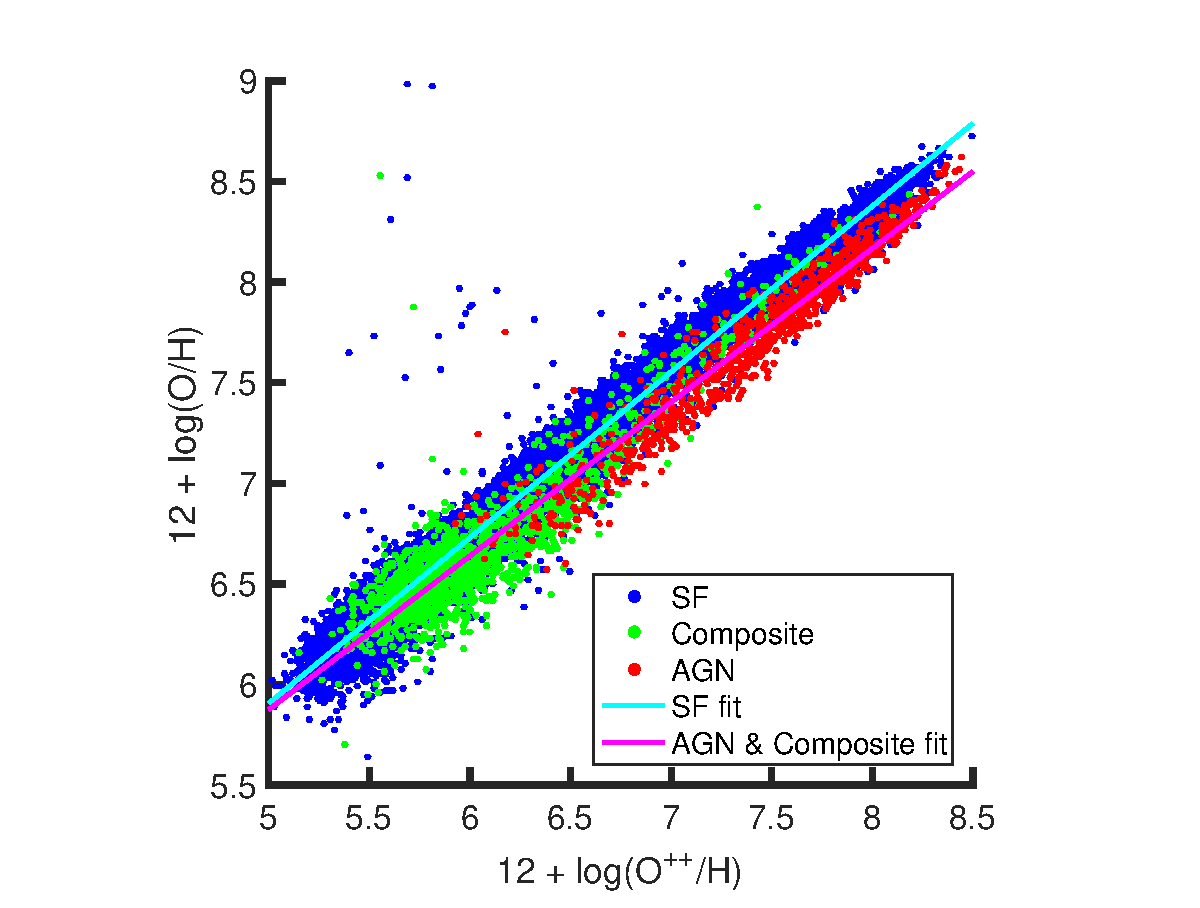
\includegraphics[width=0.75\textwidth]{Images/Paper3/Zlow_v_Zreal_1sig_I06_BPTclass_fits}
    \caption[O$^++$/H versus O/H]{$12 + \log{\text{O}^{++}/\text{H}}$ versus \OH 
    for those galaxies with $M_r > -20$ as calculated with the direct method; 
    the galaxies are colored by their classification in the BPT diagrams 
    \citep[from][]{Brinchmann04}.  Two linear models have been fit to three 
    groups in the sample: star-forming and AGN/composite galaxies; the best fit 
    parameters can be found in Table \ref{tab:ab}.}
    \label{fig:lowVreal}
\end{figure}

We derive an ICF for O$^+$ to overcome some limitations on the observations of 
dwarf galaxies in SDSS to bolster our sample size.  Because we are studying 
dwarf galaxies, the [\ion{O}{2}] $\lambda 3727$ doublet necessary for estimating 
the abundance of O$^+$ is only available for objects within the redshift range 
$0.02 < z < 0.03$ \citep[see Sec. \ref{sec:SDSS_limits_P3} and][for more 
details]{Douglass17a}.  To be able to study SDSS galaxies at redshifts less than 
0.02, we need to find an alternate way to estimate the abundance of O$^+$.  
Ordinarily, we would use an ICF to replace the missing ionization stage, as 
outlined in Sec. \ref{sec:DirectTe} for the nitrogen abundance.  Because the 
[\ion{O}{2}] $\lambda 3727$ emission line is normally available for analysis, 
there are no approximations available for the ICF for the amount of 
singly-ionized oxygen.  To construct an ICF appropriate for our dwarf galaxy 
sample, we compare \OH to $12 + \log{\text{O}^{++}/\text{H}}$ as calculated by 
the Direct $T_e$ method for all galaxies in SDSS with $M_r > -20$.  Recognizing 
that the relative amounts of singly- and doubly-ionized oxygen will depend on 
the hardness of a galaxy's spectrum, we use a Baldwin-Phillips-Terlevich (BPT) 
diagram \citep{Baldwin81} to classify each galaxy as star-forming, AGN, or 
composite (containing characteristics of both a star-forming region and an AGN).  
Noting a strong separation in the relationship between O$^{++}$/H and O/H with 
respect to the galaxies' BPT classifications by \cite{Brinchmann04}, we fit two 
linear models to the sample, seen in Fig. \ref{fig:lowVreal} and defined as 
\begin{equation}\label{eq:fit}
    12 + \log{\text{O}/\text{H}} = a(12 + \log{\text{O}^{++}/\text{H}}) + b
\end{equation}
The values for $a$ and $b$ for the two classes are listed in Table \ref{tab:ab}.



\begin{table}
\centering

    \begin{tabular}{l|c|c|c}
         & SF (dwarf) & SF ($M_r > -20$) & AGN \& Composite\\
        \hline
        $a$ & $0.84 \pm 0.013$ & $0.824 \pm 0.0010$ & $0.764 \pm 0.0035$\\
        $b$ & $1.61 \pm 0.094$ & $1.787 \pm 0.0065$ & $2.05 \pm 0.023$
    \end{tabular}
    
    \caption[Coefficients of oxygen abundance fits]{Coefficients for the linear 
    trends (Eqn. \ref{eq:fit}) fit to the SF galaxies (dwarf and those with 
    $M_r > -20$) and AGN and composite galaxies.  With these trends, we can now 
    calculate the total oxygen abundance for a galaxy with knowing only the 
    O$^{++}$/H abundance.}
    
    \label{tab:ab}
    
\end{table}



As expected, the star-forming galaxies have less doubly ionized oxygen than 
both the composite and AGN galaxies.  Since the degree of ionization depends on 
the temperature of the stars ionizing the gas, this means that the star-forming 
galaxies have cooler ionizing sources than the composite and AGN galaxies.

For those star-forming dwarf galaxies for which [\ion{O}{2}] $\lambda$3727 is 
not observed in the SDSS spectra, we use the coefficients for the star-forming 
dwarf galaxies with Eqn. \ref{eq:fit} to calculate the total oxygen abundance in 
the galaxy based on the amount of doubly-ionized oxygen found with Eqn. 4 of 
\cite{Douglass17a}.  While we list the coefficients for the linear models of 
both those galaxies with absolute magnitudes $-17 > M_r > -20$ and the AGN and 
composite galaxies in Table \ref{tab:ab}, we do not use them to calculate the 
chemical abundances of these galaxies for the reasons outlined in Section 
\ref{sec:DirectTe}.



%%%%%%%%%%%%%%%%%%%%%%%%%%%%%%%%%%%%%%%%%%%%%%%%%%%%%%%%%%%%%%%%%%%%%%%%%%%%%%%%
%
%    DATA
%
%%%%%%%%%%%%%%%%%%%%%%%%%%%%%%%%%%%%%%%%%%%%%%%%%%%%%%%%%%%%%%%%%%%%%%%%%%%%%%%%
\section[SDSS Data]{SDSS data and galaxy selection}

The SDSS Data Release 7 (DR7) \citep{Abazajian09} is a wide-field multiband 
imaging and spectroscopic survey employing a drift scanning technique to map 
approximately one-quarter of the northern sky.  Photometric data in the 
five-band SDSS system --- $u$, $g$, $r$, $i$, and $z$ --- are taken with a 
dedicated 2.5-meter telescope at the Apache Point Observatory in New Mexico 
\citep{Fukugita96, Gunn98}.  Follow-up spectroscopic analysis is performed on 
galaxies with a Petrosian $r$-band magnitude $m_r < 17.77$ \citep{Lupton01, 
Strauss02}.  The spectra are taken using two double fiber-fed spectrometers and 
fiber plug plates with a minimum fiber separation of 55"; the observed 
wavelength range is $3800\text{\AA}$ to $9200\text{\AA}$ with a resolution 
$\lambda / \Delta \lambda \sim$1800 \citep{Blanton03}.  We use emission-line 
flux data from the MPA-JHU value-added catalog\footnote{Available at 
\url{http://www.mpa-garching.mpg.de/SDSS/DR7/}}, which is based on the SDSS DR7 
sample of galaxies.  All flux values have been corrected for dust reddening with 
the \cite{Cardelli89} extinction curve as implemented in pyNeb 
\citep{Luridiana15}; we assume the theoretical ratio H$\alpha$/H$\beta = 2.86$ 
at 10,000 K and 100 cm$^{-3}$ \citep{Osterbrock89}.

We use the stellar mass estimates from the NASA-Sloan Atlas \citep{Blanton11}.  
The \ion{H}{1} mass estimates are from the 70\% complete ALFALFA catalog 
$\alpha.70$ \citep{Giovanelli05}; \ion{H}{1} detections were matched to the SDSS 
galaxies by locating the nearest optical counterpart identified in the 
$\alpha.70$ catalog within 1 arcmin.  Absolute magnitudes, colors, and all other 
additional data are from the KIAS value-added galaxy catalog 
\citep{Choi10,Blanton05}.  Galaxy colors are rest-frame colors which have been 
$K$-corrected to a redshift of 0.1; they are corrected for galactic extinction 
and calculated with model magnitudes.  All galaxies have been visually inspected 
to remove any galaxy fragments or duplicates.


%-------------------------------------------------------------------------------
\subsection{Spectroscopic selection}\label{sec:SDSS_limits_P3}

We employ the same requirements for our sample as in 
\cite{Douglass17a,Douglass17b}: all galaxies must have
\begin{enumerate}
    \item{$M_r > -17$ (dwarf galaxies);}
    \item{a minimum $5\sigma$ detection of H$\beta$;}
    \item{a minimum $1\sigma$ detection of [\ion{O}{3}] $\lambda 4363$;}
    \item{a flux $> 0$ for [\ion{O}{2}] $\lambda 3727$, [\ion{O}{3}] $\lambda \lambda 4959,5007$, and [\ion{N}{2}] $\lambda \lambda 6548,6584$;}
    \item{$T(\text{[\ion{O}{3}]}) > 3\times 10^4 \text{ K}$;}
    \item{a star-forming BPT classification by \cite{Brinchmann04}.}
\end{enumerate}

For those galaxies with a redshift $z \gtrsim 0.02$, we use the 
\texttt{oii\_flux} value from the MPA-JHU catalog in place of their [\ion{O}{2}] 
$\lambda \lambda 3726,3729$ flux measurement.  See \cite{Douglass17a} for 
further details on each of these requirements.


%-------------------------------------------------------------------------------
\subsection{Void classification}

The large-scale environment of the galaxies is determined using the void catalog 
compiled by \cite{Pan12}, which was constructed with the galaxies in SDSS DR7 
catalog.  The VoidFinder algorithm of \cite{Hoyle02} \citep[based on the 
algorithm described by][]{ElAd97} removes all isolated galaxies (defined as 
having the third nearest neighbor more than 7 \hMpc away) using only galaxies 
with absolute magnitudes $M_r < -20$.  After applying a grid to the remaining 
galaxies, spheres are grown from all cells containing no galaxies until it 
encounters four galaxies on its surface.  A sphere must have a minimum 10 \hMpc 
radius to be classified as a void (or part of one).  If two spheres overlap by 
more than 10\%, they are considered part of the same void.  See \cite{Hoyle02} 
for a more detailed description of the VoidFinder algorithm.  Those galaxies 
that fall within these void spheres are classified as voids.  Galaxies that lie 
outside the spheres are classified as wall galaxies.  Because we cannot identify 
any voids within 5 \hMpc of the edge of the survey, we classify these galaxies 
as ``Uncertain.''

Of the $\sim$800,000 galaxies with spectra available in SDSS DR7, 9519 are 
dwarf galaxies.  Applying the spectroscopic cuts, our sample includes 993 void 
dwarf galaxies and 759 wall dwarf galaxies.


%%%%%%%%%%%%%%%%%%%%%%%%%%%%%%%%%%%%%%%%%%%%%%%%%%%%%%%%%%%%%%%%%%%%%%%%%%%%%%%%
%
%    ANALYSIS & RESULTS
%
%%%%%%%%%%%%%%%%%%%%%%%%%%%%%%%%%%%%%%%%%%%%%%%%%%%%%%%%%%%%%%%%%%%%%%%%%%%%%%%%
\section[Analysis \& Results]{Abundance analysis and results}

Our primary objective is to perform a relative measurement of gas-phase 
abundances of dwarf galaxies to discern how their chemical evolution is affected 
by the large-scale environment.

All line ratios listed are ratios of the emission-line fluxes.  Galaxies with 
low metallicities have $Z =$ \OH $< 7.6$ \citep{Pustilnik06}; galaxies with high 
metallicities have $Z > 8.2$ \citep{Pilyugin06}.  The solar metallicity 
$Z_\odot = 8.86$ \citep{Delahaye06}.


%-------------------------------------------------------------------------------
\subsection{Estimation of uncertainties}

% Uncertainties
Uncertainties in the computed abundances are estimated using a Monte-Carlo 
method.  Using the measured line fluxes and scaled uncertainty estimates, we 
calculate 100,000 abundance estimates.  For each abundance estimate, a new 
positive ``fake'' line flux is drawn from a normal distribution.  We use the 
standard deviation in these sets of 100,000 calculated abundance values for the 
error in our abundance estimate.  See \cite{Douglass17a} for a more in-depth 
description of this process.


%-------------------------------------------------------------------------------
\subsection{Sources of systematic error}

Many physical properties of galaxies exhibit a radial dependence \citep{Bell00}.  
As a result, abundance estimates can depend on where the spectroscopic fiber is 
placed on the galaxy.  The estimated abundance will not necessarily be 
representative of a global abundance value if not all of the galaxy's light is 
contained within the fiber.  \cite{Belfiore17} show that both the metallicity 
and N/O ratio gradients are relatively flat for lower mass galaxies 
($\log(M/M_\odot) = 9$) and steepen with increasing stellar mass.  In SDSS DR7, 
the spectroscopic fiber diameter is 3"; this corresponds to a minimum physical 
diameter of 1.31 $h^{-1}$kpc at a redshift $z < 0.03$.  For most of the dwarf 
galaxies in this study, this contains the majority of their angular size.  
Assuming the abundance gradients remain flat for dwarf galaxies as suggested by 
the results of \cite{Belfiore17}, then our estimates of the gas-phase chemical 
abundances for our sample of dwarf galaxies are independent of the location of 
the spectral fiber on the galaxies' surfaces.

The selection criteria outlined in Section \ref{sec:SDSS_limits_P3} limit our 
sample to only star-forming dwarf galaxies.  As a result, this is not a 
representative sample of the entire dwarf galaxy population.  We are only able 
to discuss the influence of the large-scale environment on star-forming dwarf 
galaxies in this study.  Unfortunately, it is impossible to estimate the 
chemical abundances of red dwarf galaxies with the direct $T_e$ method because 
the UV photons from young stars are needed to excite the interstellar gas.


%-------------------------------------------------------------------------------
\subsection{Dwarf galaxy abundances}

% Results table (machine-readable)
\begin{sidewaystable}
\centering

\begin{tabular}{cccccccccccc}
Index\footnote{KIAS-VAGC galaxy index number} & R.A. & Decl. & Redshift & $M_r$ & \multicolumn{2}{c}{$12 + \log \left( \frac{\text{O}}{\text{H}} \right)$} & \multicolumn{2}{c}{$12 + \log \left( \frac{\text{N}}{\text{H}} \right)$} & \multicolumn{2}{c}{$\log \left( \frac{\text{N}}{\text{O}} \right)$} & Void/Wall \\
\hline \\
63713 & \RA{09}{20}{04}{.27} & -\dec{00}{30}{08}{.97} & 0.0257 & -16.73 & 7.80 & $\pm$0.41 & 6.83 & $\pm$0.28 & -0.97 & $\pm$0.49 & Wall \\
73537 & \RA{09}{25}{24}{.23} & +\dec{00}{12}{40}{.39} & 0.0250 & -16.94 & 7.94 & $\pm$0.34 & 6.76 & $\pm$0.24 & -1.18 & $\pm$0.41 & Wall \\
75442 & \RA{13}{13}{24}{.25} & +\dec{00}{15}{02}{.95} & 0.0264 & -16.81 & 7.55 & $\pm$0.35 & 6.73 & $\pm$0.24 & -0.82 & $\pm$0.42 & Void \\
168874 & \RA{11}{45}{13}{.16} & -\dec{01}{48}{17}{.68} & 0.0273 & -16.99 & 8.16 & $\pm$0.31 & 6.94 & $\pm$0.21 & -1.21 & $\pm$0.37 & Wall \\
184308 & \RA{09}{39}{09}{.38} & +\dec{00}{59}{04}{.15} & 0.0244 & -16.73 & 7.36 & $\pm$0.43 & 6.71 & $\pm$0.31 & -0.65 & $\pm$0.53 & Wall\\
\end{tabular}

\caption[Chemical abundances of subset of 135 dwarf galaxies]{Five of the 135 dwarf galaxies analyzed from SDSS DR7.  The flux values for all required emission lines can be found in the MPA-JHU value-added catalog.  Metallicity values are calculated using the direct $T_e$ method, with error estimates via a Monte Carlo method.  The void catalog of \cite{Pan12} is used to classify the galaxies as either Void or Wall.  If a galaxy is located too close to the boundary of the SDSS to identify whether or not it is inside a void, it is labeled as Uncertain.  (This table is available in its entirety in machine-readable form.)}

\label{tab:Results_P2}

\end{sidewaystable}


The abundances estimated using the direct $T_e$ method for our dwarf galaxy 
sample are listed in Table \ref{tab:Results_P3}.  Also included are other 
significant characteristics and identification for the galaxies, including their 
large-scale environmental classification.


\subsubsection{Oxygen and nitrogen abundances}

\begin{figure*}
    \centering
    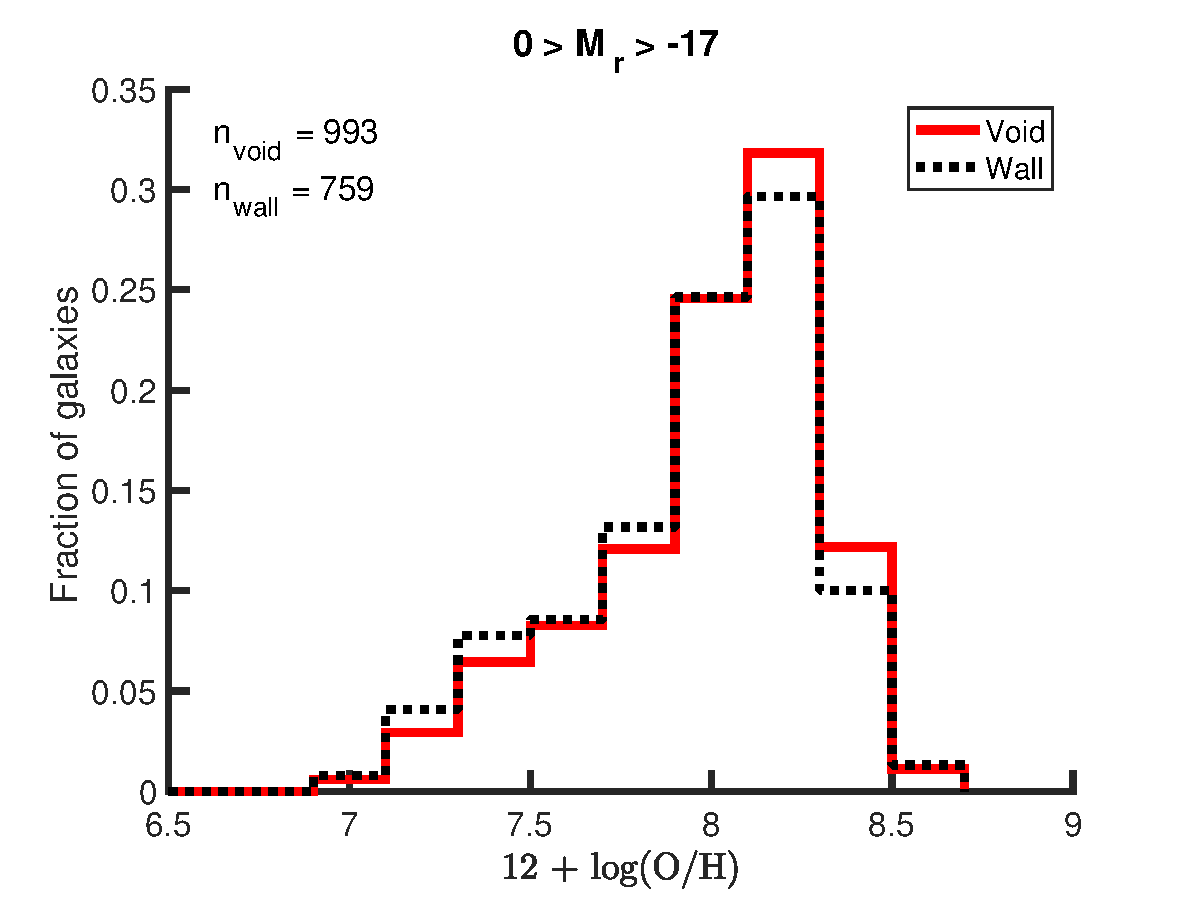
\includegraphics[width=0.49\textwidth]{Images/Paper3/1sig_dwarf_SF_t3_12logOHrelations_dust_hist}
    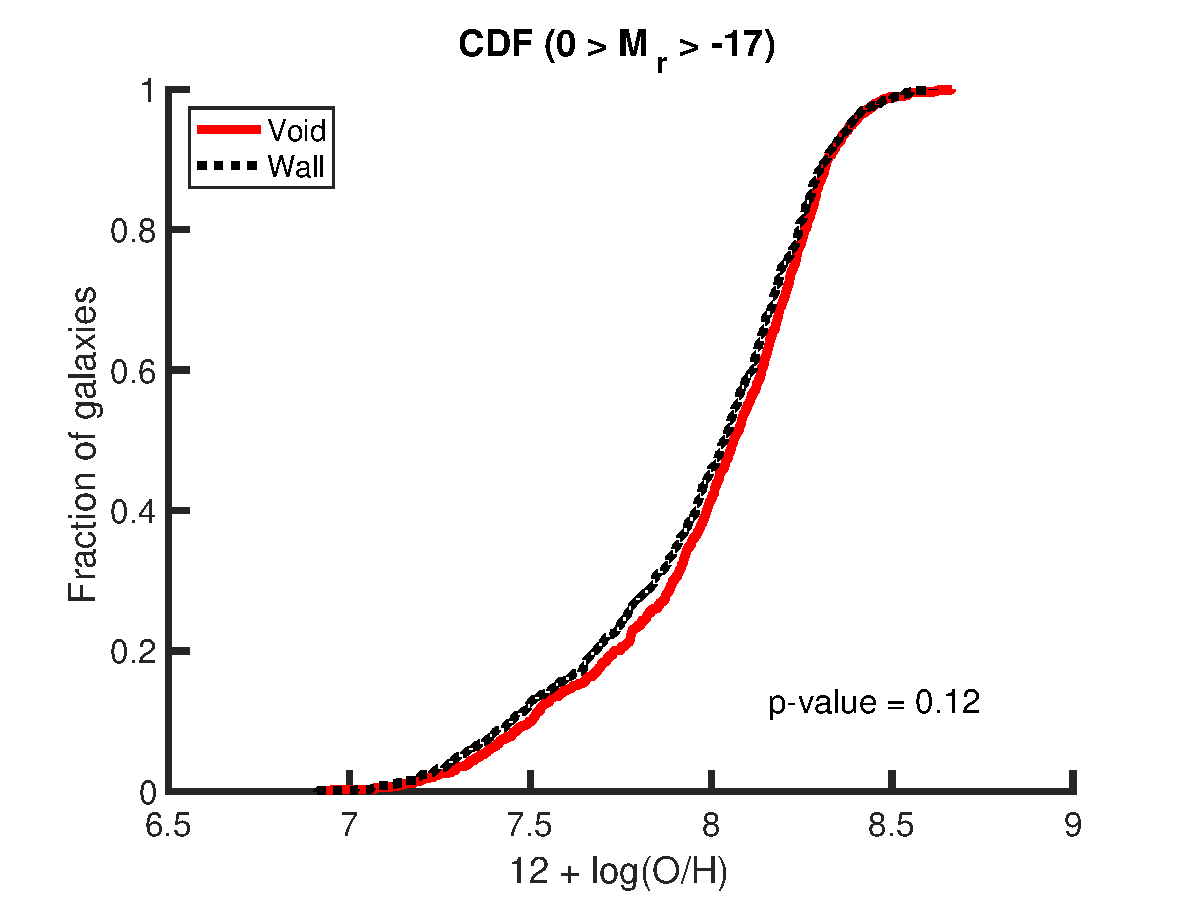
\includegraphics[width=0.49\textwidth]{Images/Paper3/1sig_dwarf_SF_t3_12logOHrelations_dust_CDF}
    \caption[O/H distribution for dwarf galaxy sample]{Gas-phase metallicity of 
    void dwarf (red solid line) and wall dwarf (black dashed line) galaxies.  A 
    two-sample K-S test of the two data sets results in an asymptotic $p$-value 
    of 0.12, indicating a 12\% probability that a test statistic greater than 
    the observed value of 0.06 will be seen if the void sample is drawn from the 
    wall sample.  This is reflected visually, as there appears to be a slight 
    but statistically significant significant large-scale environmental 
    influence on the metallicity of dwarf galaxies.}
    \label{fig:met1sig_P3}
\end{figure*}

\begin{figure*}
    \centering
    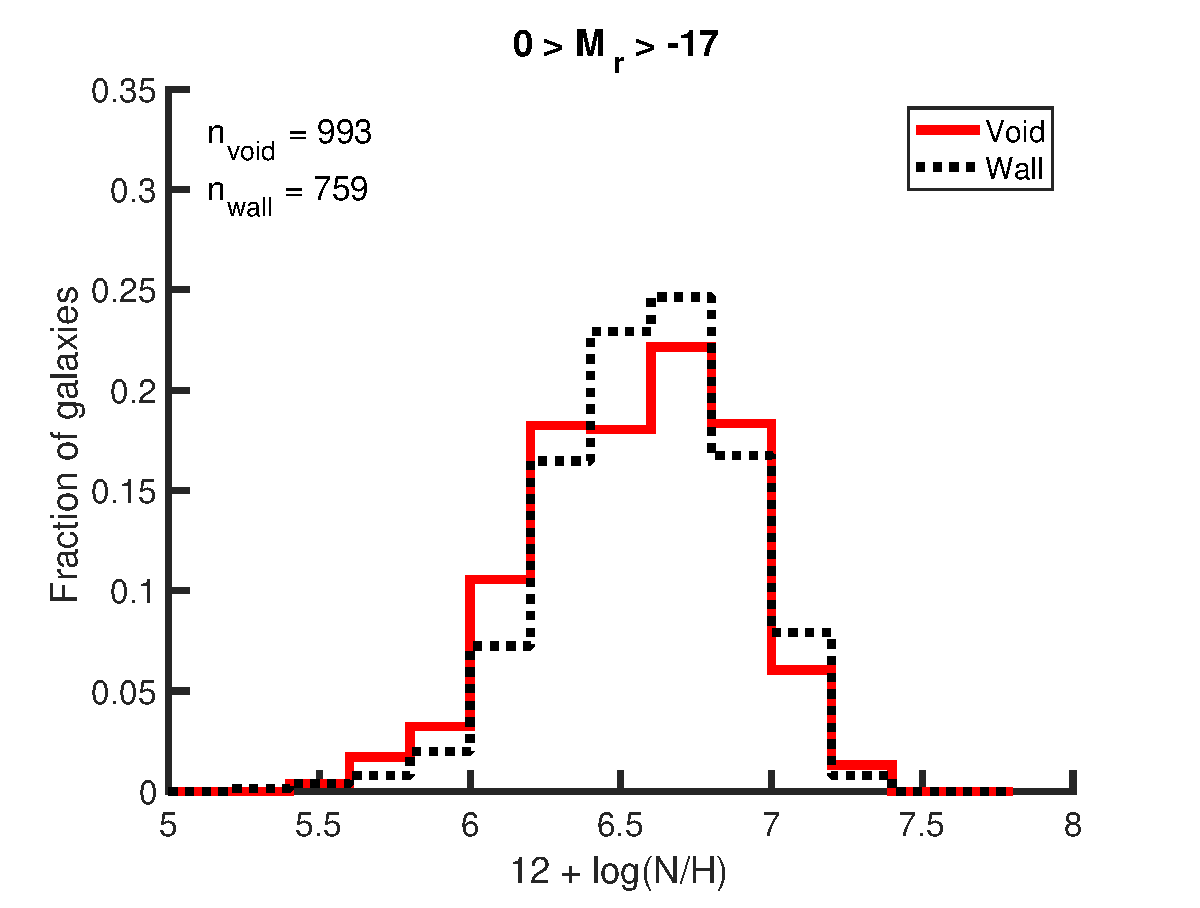
\includegraphics[width=0.49\textwidth]{Images/Paper3/1sig_dwarf_SF_t3_12logNHrelations_dust_hist}
    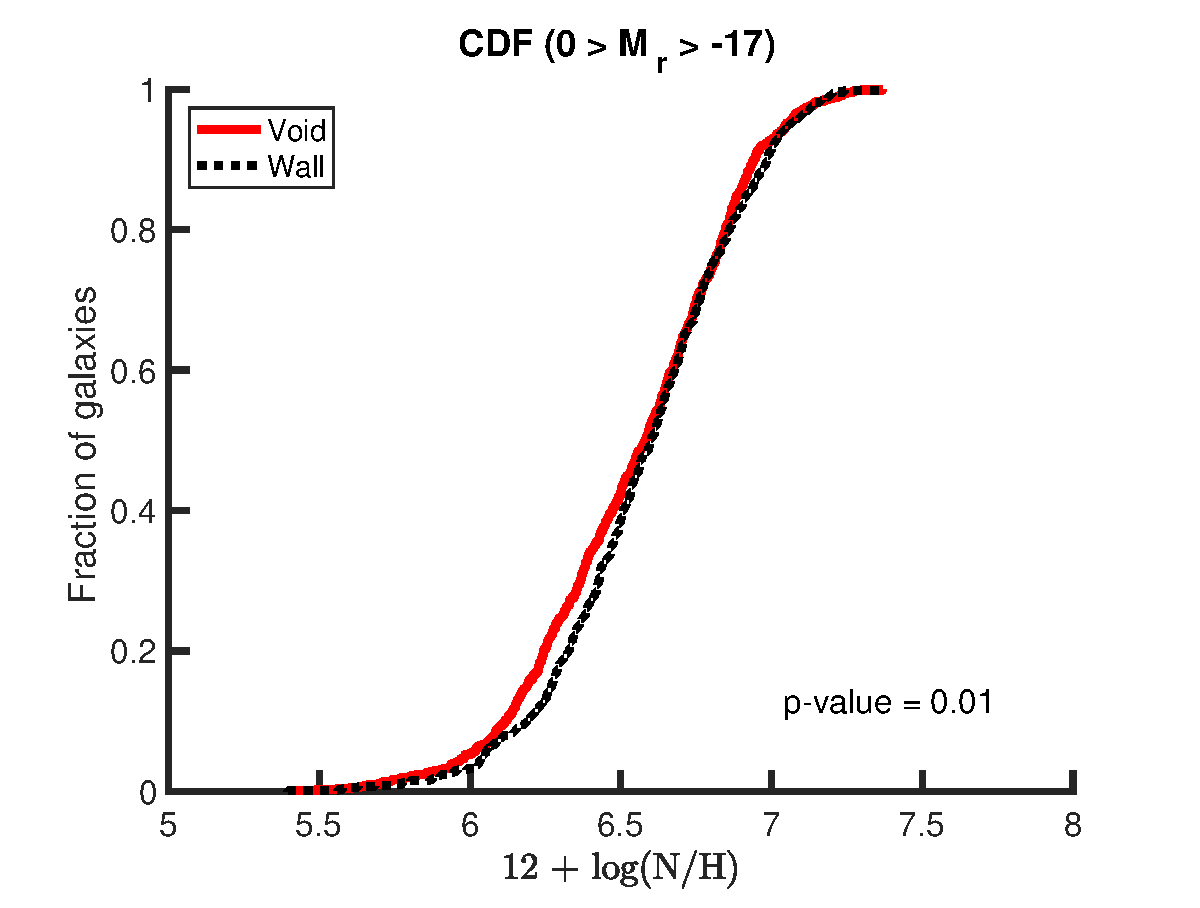
\includegraphics[width=0.49\textwidth]{Images/Paper3/1sig_dwarf_SF_t3_12logNHrelations_dust_CDF}
    \caption[N/H distribution for dwarf galaxy sample]{Abundance of nitrogen 
    relative to hydrogen of void dwarf (red solid line) and wall dwarf (black 
    dashed line) galaxies.  A two-sample K-S test of the two data sets results 
    in an asymptotic $p$-value of 0.015, indicating a 1.5\% probability that a 
    test statistic greater than the observed value of 0.08 will be seen, if the 
    void sample is drawn from the wall sample.  This is reflected visually, as 
    the void dwarf galaxies appear to have lower values of the N/H ratio than 
    the wall dwarf galaxies.  There is a large-scale environmental dependence of 
    the chemical evolution of dwarf galaxies.}
    \label{fig:N_1sig_P3}
\end{figure*}

The distributions of oxygen and nitrogen abundances for dwarf galaxies as a 
function of large-scale environment are shown in Figures \ref{fig:met1sig_P3} 
and \ref{fig:N_1sig_P3}, respectively.  Both histograms show a slight shift 
between voids and walls in the chemical abundances of dwarf galaxies.  A 
two-sample Kolmogorov-Smirnov (K-S) test quantifies this observation --- a test 
statistic of 0.06 for oxygen and 0.08 for nitrogen are produced, corresponding 
to a probability of 12\% and 1.5\%, respectively, that a test statistic greater 
than or equal that observed will be measured if the void sample were drawn from 
the wall sample.  The cumulative distribution function (CDF) for each of these 
elements can be seen on the right in Figures \ref{fig:met1sig_P3} and 
\ref{fig:N_1sig_P3}; they show that void dwarf galaxies have slightly higher 
oxygen abundances and slightly lower nitrogen abundances than dwarf galaxies in 
more dense regions.  The K-S test quantifies the visual interpretation of these 
figures that the distributions of oxygen and nitrogen abundances are slightly 
different for star-forming dwarf galaxies in voids and walls.

The average and median values of the dwarf galaxy abundances also indicate a 
shift as a result of the large-scale environment.  The average oxygen abundance 
for void dwarf galaxies is $7.99\pm 0.007$ and the median is 8.06, while the 
average oxygen abundance for wall dwarf galaxies is $7.96\pm 0.009$ with a 
median value of 8.04.  This implies that the void dwarf galaxies have higher 
oxygen abundances by about 7\% (average shift of $0.03\pm 0.012$; median shift 
of 0.03) relative to wall dwarf galaxies.  In contrast, the average nitrogen 
abundance for void dwarf galaxies is only $6.55\pm 0.007$ with a median of 6.58, 
while the wall dwarf galaxies have an average nitrogen abundance of 
$6.58\pm 0.008$ and a median of 6.60.  The void dwarf galaxies have lower 
nitrogen abundances by about 10\% (an average shift of $0.04\pm 0.011$ and a 
median shift of 0.02) relative to wall dwarf galaxies.  A tabular version of 
this analysis can be found in Table \ref{tab:stats_p3}.


\subsubsection{Ratio of nitrogen to oxygen}

\begin{figure*}
    \centering
    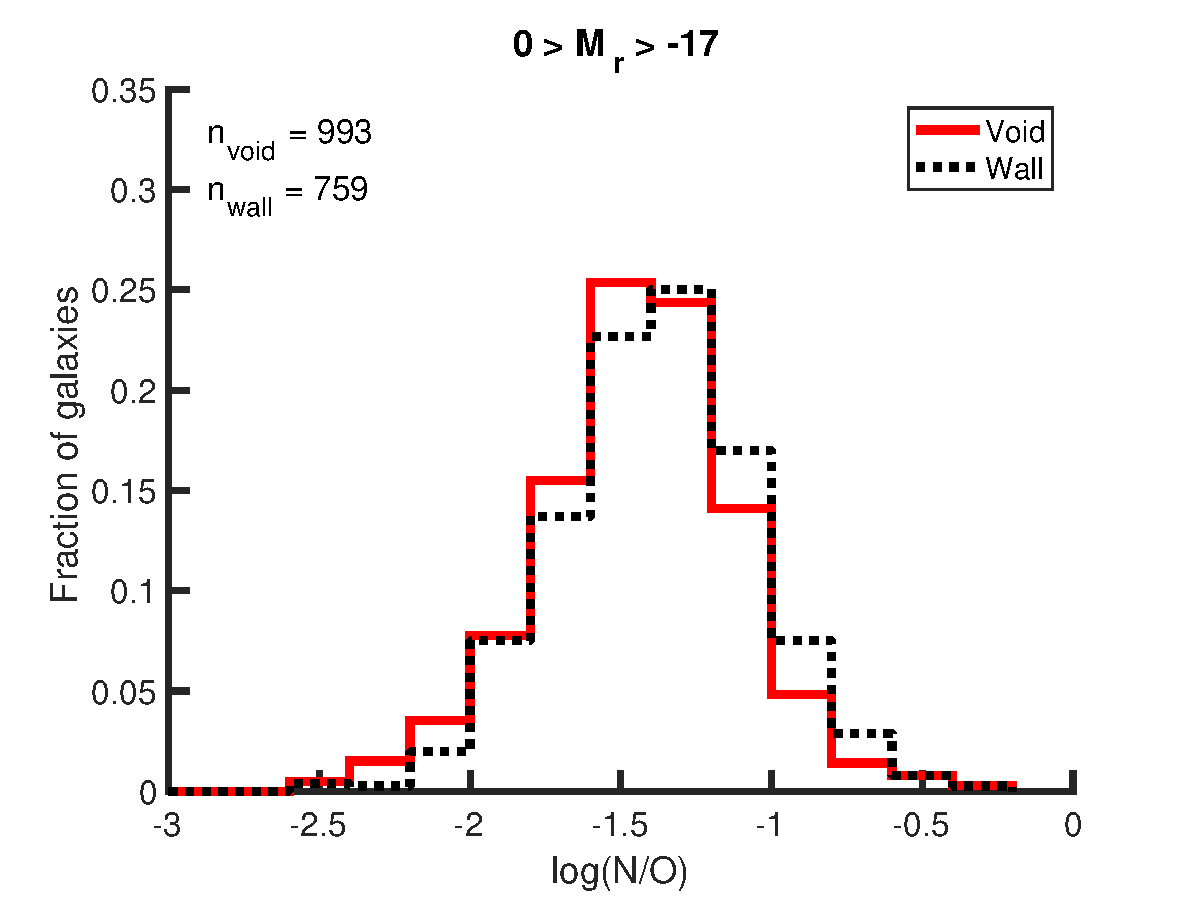
\includegraphics[width=0.49\textwidth]{Images/Paper3/1sig_dwarf_SF_t3_logNOrelations_dust_hist}
    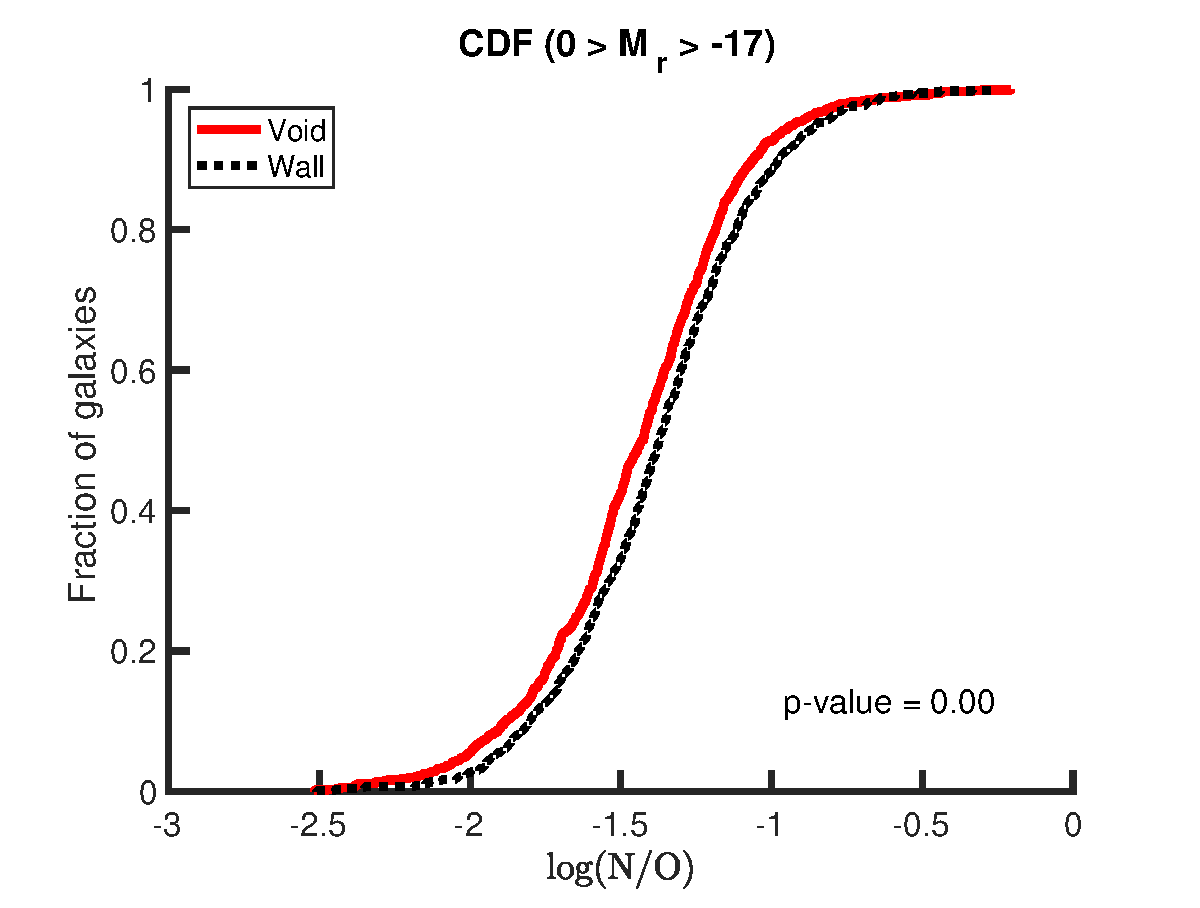
\includegraphics[width=0.49\textwidth]{Images/Paper3/1sig_dwarf_SF_t3_logNOrelations_dust_CDF}
    \caption[N/O distribution of dwarf galaxy sample]{Ratio of nitrogen to 
    oxygen of void dwarf (red solid line) and wall dwarf (black dashed line) 
    galaxies.  A two-sample K-S test of the two data sets results in an 
    asymptotic $p$-value of $2.6\times 10^{-4}$, indicating only a 0.03\% 
    probability that a test statistic greater than the observed value of 0.10 
    will be seen.  This is reflected visually, as there is a shift in the N/O 
    ratio between the two populations of dwarf galaxies --- the void galaxies 
    have a lower value of N/O than the wall galaxies.  There is a large-scale 
    influence on the relative chemical abundances of dwarf galaxies.}
    \label{fig:NOratio_P3}
\end{figure*}

The ratio of nitrogen to oxygen is also important to investigate, as it 
communicates the nucleosynthesis history of the galaxies.  As seen in Fig. 
\ref{fig:NOratio_P3}, the N/O abundance ratio also indicates a large-scale 
environmental influence on the chemical evolution of dwarf galaxies --- void 
dwarf galaxies have lower N/O ratios than dwarf galaxies in denser regions.  
This difference is quantified in the K-S test: the test returned a probability of 
only 0.03\% that a test statistic greater than or equal to 0.10 will be measured 
if the void sample was drawn from the wall sample.  The distribution of N/O 
abundance ratios for void dwarf galaxies is lower by about 17\% (an average 
shift of $0.07\pm 0.016$ and a median shift of 0.06) relative to the 
distribution of N/O ratios in wall dwarf galaxies.


% Statistics table
\begin{table}
    \centering
    
    \begin{tabular}{ccccccc}
        Environment & Average & Median & Average Shift\footnote{Wall -- Void (Positive shifts indicate that the wall values are greater than the void values; negative shifts indicate that the void values are greater than the wall values.)\label{fnote_P3}} & Median Shift\textsuperscript{\ref{fnote_P3}} & $p$-value & K-S Test Statistic\\
        \hline
        % Oxygen %%%%%%%%%%%%%%%%%%%%%%%%%%%%%%%%%%%%%%%%%%%%%%%%%%%%%%%%%%%%%%%
        \hline
        \multicolumn{7}{c}{\OH}\\
        \hline
        Void & $7.99\pm 0.007$ & 8.06 & \multirow{2}{*}{$-0.03\pm 0.012$} & \multirow{2}{*}{-0.03} & \multirow{2}{*}{0.1197} & \multirow{2}{*}{0.0569}\\
        Wall & $7.96\pm 0.009$ & 8.04 & & & & \\
        % Nitrogen %%%%%%%%%%%%%%%%%%%%%%%%%%%%%%%%%%%%%%%%%%%%%%%%%%%%%%%%%%%%
        \hline
        \multicolumn{7}{c}{\NH}\\
        \hline
        Void & $6.55\pm 0.007$ & 6.58 & \multirow{2}{*}{$0.04\pm 0.011$} & \multirow{2}{*}{0.02} & \multirow{2}{*}{0.0149} & \multirow{2}{*}{0.0750}\\
        Wall & $6.58\pm 0.008$ & 6.60 & & & & \\
        % N/O %%%%%%%%%%%%%%%%%%%%%%%%%%%%%%%%%%%%%%%%%%%%%%%%%%%%%%%%%%%%%%%%%
        \hline
        \multicolumn{7}{c}{\NO}\\
        \hline
        Void & $-1.45\pm 0.010$ & -1.43 & \multirow{2}{*}{$0.07\pm 0.016$} & \multirow{2}{*}{0.06} & \multirow{2}{*}{0.0003} & \multirow{2}{*}{0.1013}\\
        Wall & $-1.38\pm 0.012$ & -1.37 & & & & \\
    \end{tabular}
    
    \caption[Abundance statistics of full dwarf galaxy sample]{Statistics on the 
    gas-phase oxygen, nitrogen, and nitrogen relative to oxygen abundances in 
    dwarf void and wall galaxies.  Combined with the histograms in Figures 
    \ref{fig:met1sig_P3}--\ref{fig:NOratio_P3}, these results indicate an 
    influence on the chemical evolution of galaxies by the large-scale 
    environment, especially on the relative abundance of nitrogen to oxygen.  
    Void galaxies have slightly higher oxygen and nitrogen abundances than wall 
    galaxies, but void galaxies have slightly lower N/O ratios than wall 
    galaxies.}
    
    \label{tab:stats_p3}
    
\end{table}


%-------------------------------------------------------------------------------
\subsection{Comparison to previously published oxygen abundance estimates}
% Compare to Tremonti et al. (2004)

\begin{figure}
    \centering
    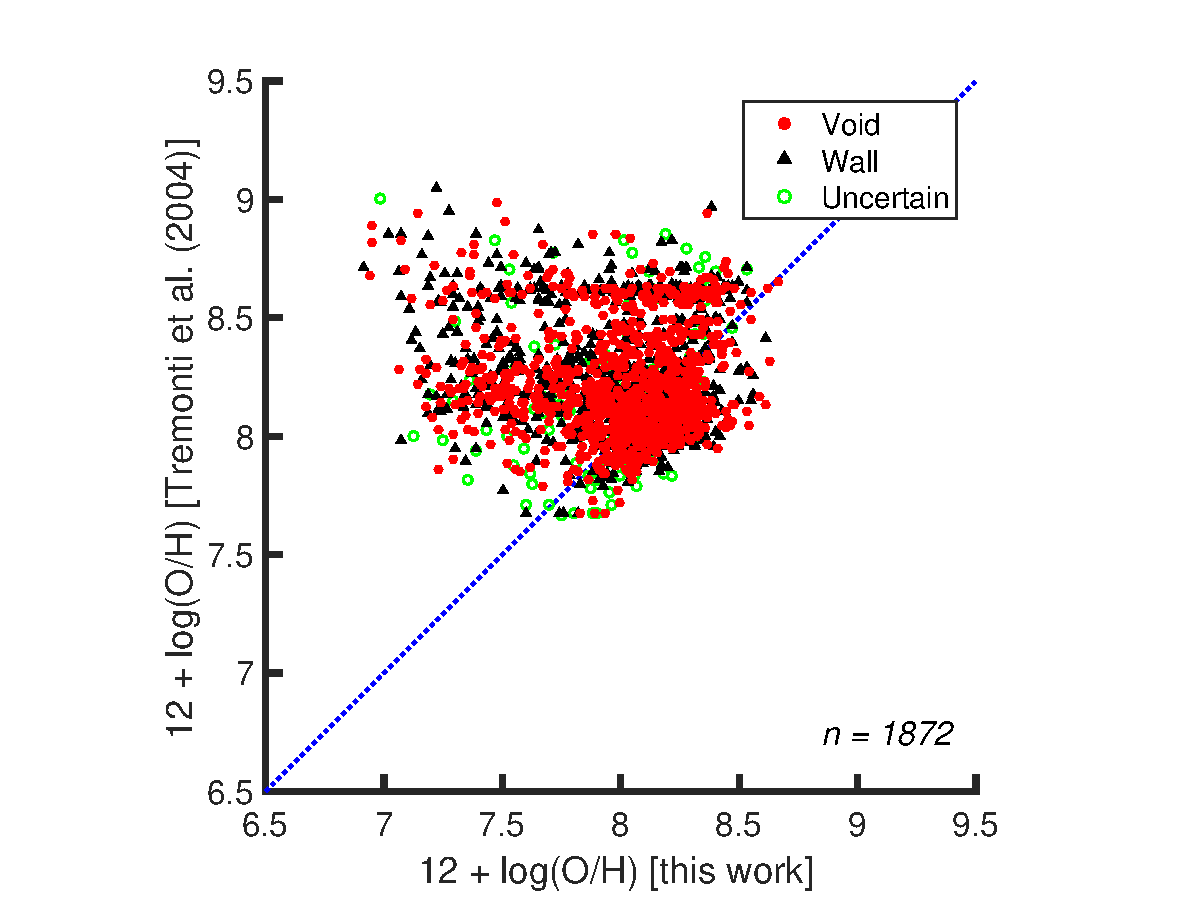
\includegraphics[width=0.75\textwidth]{Images/Paper3/1sig_dwarf_I06relations_SF_t3_T04comparison_dust}
    \caption[Comparison of O$^+$ approximation metallicities to 
    \cite{Tremonti04}]{Oxygen abundance comparison between our calculated 
    estimates with the O$^+$ approximation and those made by \cite{Tremonti04}.  
    Error bars have been omitted for clarity.  While the majority of our 
    abundance estimates agree reasonably well with the values already published, 
    it is clear that our estimates are often lower than the previously published 
    values.  It is well known that the strong-line methods \citep[like those 
    used by][]{Tremonti04} overestimate the oxygen abundance by as much as 0.3 
    dex \citep{Kennicutt03}.  Therefore, it is not surprising that the oxygen 
    abundances measured using the direct $T_e$ method are lower, particularly at 
    very low metallicities.}
    \label{fig:T04_comp}
\end{figure}

While no estimates of the nitrogen or N/O abundances have been made on a large 
selection of the SDSS galaxies, we can compare our oxygen abundance estimates to 
the metallicity values measured by \cite{Tremonti04}.  While we both use data 
from the MPA-JHU value-added catalog, \cite{Tremonti04} employs an empirical 
method to calculate the metallicity that is based on calibrated relationships 
between direct $T_e$ methods and strong-line ratios.  The results of this 
comparison are shown in Fig. \ref{fig:T04_comp}.  While the majority of our 
abundance estimates agree reasonably well with the values calculated by 
\cite{Tremonti04}, it is also clear that our estimates often predict abundances 
lower than those previously published.  This is especially true for the low 
metallicity regime ($12 + \log \left(\text{O}/\text{H}\right) < 7.6$).  Methods 
which are based on calibrations rarely use low metallicity galaxies in their 
source for calibrating.  As a result, empirical methods will often overestimate 
the abundance values, especially in the low-metallicity regime.  
\cite{Kennicutt03} show that strong-line methods (methods which make extreme use 
of the strong emission lines) can overestimate the metallicity abundances by as 
much as 0.3 dex.  Therefore, we are not surprised at the apparent lack of 
correlation between our oxygen abundance estimates and those of 
\cite{Tremonti04}.


%-------------------------------------------------------------------------------
\subsection{N/O versus O/H} \label{sec:NO_OH}

\begin{figure}
    \centering
    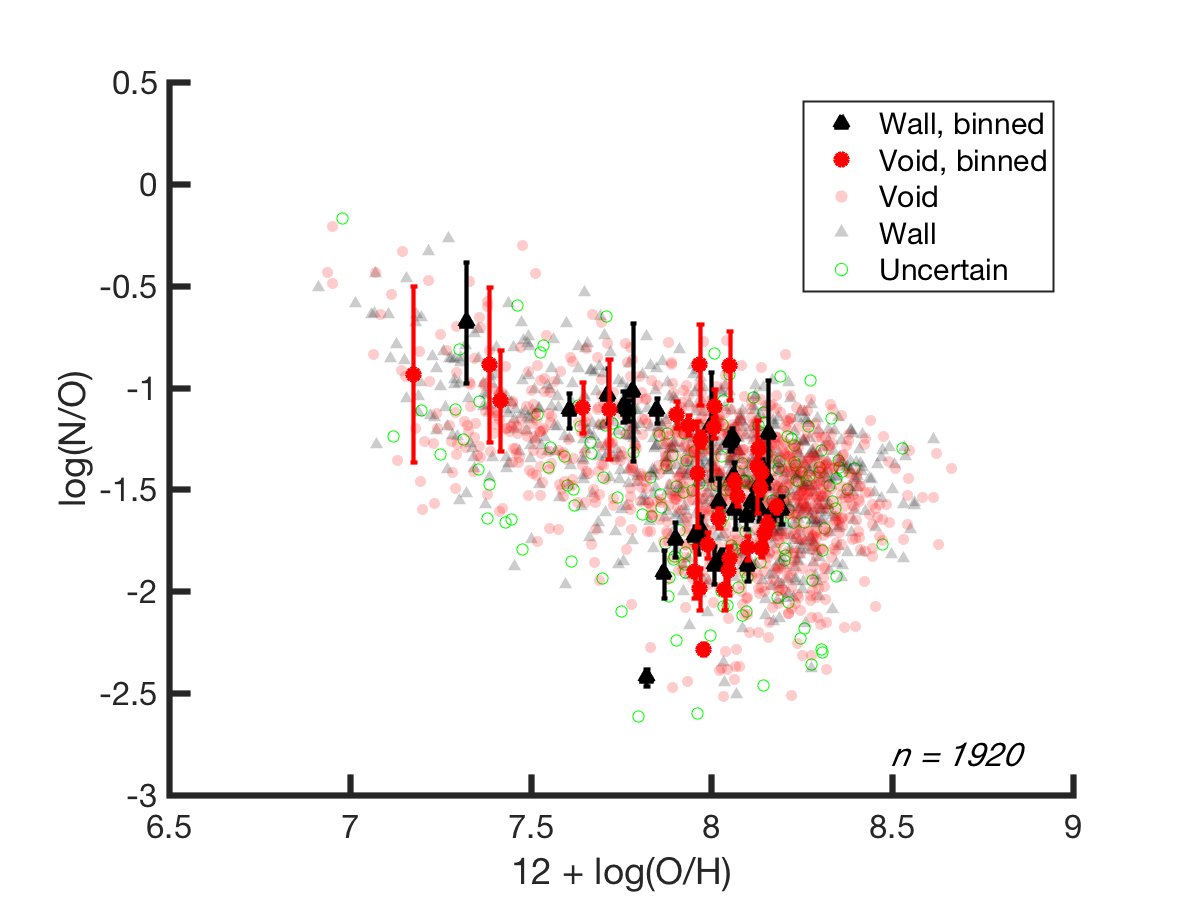
\includegraphics[width=0.75\textwidth]{Images/Paper3/1sig_I06relations_dwarf_SF_t3_dust_NSA_Z12logOH_logNO_scatterMbin}
    \caption[O/H versus N/O for star-forming dwarf galaxies]{Oxygen abundance 
    (\OH) versus the N/O ratio (\NO) for the dwarf galaxies in this study; the 
    average values of the galaxies' abundances when binned by stellar mass in 
    bins of width 0.1 are also shown.  As seen in \cite{Andrews13} and 
    \cite{Douglass17b}, while most of the mass bins are scattered together 
    around \NO $\sim$-1.5, there is a negative correlation between these two 
    abundance ratios.  There is no evidence of secondary nitrogen production in 
    this sample of star-forming dwarf galaxies, which would manifest as a 
    positive relationship between O/H and N/O at high metallicities.}
    \label{fig:NOvOH}
\end{figure}

Studying how the N/O ratio depends on the metallicity (gas-phase oxygen 
abundance) probes the nucleosynthetic production of nitrogen in stars within the 
galaxies.  It is believed that nitrogen can be produced as both a primary and 
secondary element, depending on the initial metallicity of the stars.  If there 
are enough of the heavy elements available when the stars are created (oxygen, 
carbon, etc.), then the CNO cycle can commence much earlier in the star's 
lifetime, resulting in a higher production of nitrogen than if the star is 
originally created with very few heavy elements.  If this is the case, then we 
should see no relationship between the N/O ratio and the oxygen abundance below 
a certain metallicity value (the primary nitrogen production phase); above this 
threshold metallicity, the N/O value should increase linearly with the oxygen 
abundance (the secondary nitrogen production phase).

As we see in Fig. \ref{fig:NOvOH}, there is no evidence of a secondary nitrogen 
production phase in our sample of dwarf galaxies.  This is in contrast with the 
evidence of secondary nitrogen production seen in Fig. \ref{fig:M_NO} of Sec. 
\ref{sec:Mass}; the source of this discrepancy is unclear.  The relationship 
between metallicity and the N/O ratio instead shows a large scatter with no 
clear correlation between the N/O ratio and the oxygen abundance at metallicity 
values higher than $\sim$7.9.  Below this value, we actually observe a negative 
correlation between the N/O ratio and the oxygen abundance.  This would indicate 
a constant value of nitrogen being synthesized in the galaxies independent of 
the amount of oxygen being produced.  A negative correlation similar to this was 
also observed by \cite{Andrews13} and \cite{Douglass17b}.   \cite{Andrews13} 
note that they measure a slope of -0.21 for their stellar mass-binned galaxies 
with metallicities \OH $< 8.5$, while \cite{Douglass17b} finds a slope of 
$-0.38\pm 0.078$ for dwarf galaxies.  A linear fit to our dwarf galaxy sample 
has a slope of $-0.52\pm 0.041$, steeper than any previously measured.

\begin{figure}
    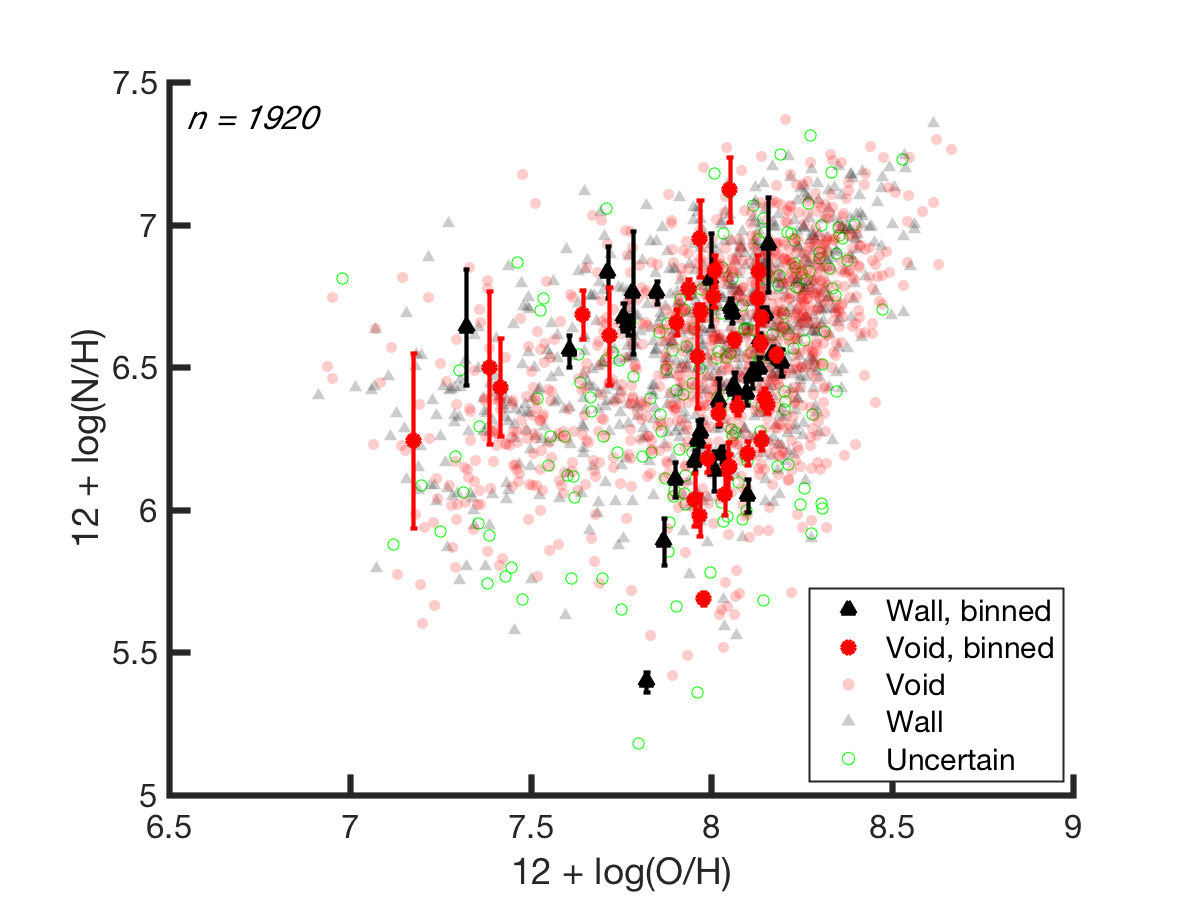
\includegraphics[width=0.75\textwidth]{Images/Paper3/1sig_I06relations_dwarf_SF_t3_dust_NSA_Z12logOH_N12logNH_scatterMbin}
    \caption[O/H versus N/H for star-forming dwarf galaxies]{Oxygen abundance 
    (\OH) versus nitrogen abundance (\NH) for the dwarf galaxies in this study; 
    the average values of the galaxies' abundances when binned by their stellar 
    mass in bins of width 0.1 are also shown.  There is evidence of two 
    evolutionary tracks for the star-forming dwarf galaxies here, one with a 
    much steeper slope than the other.}
    \label{fig:OvN_P3}
\end{figure}

Similar evidence of the nitrogen production phases can also be observed when 
looking at the relationship between the nitrogen and oxygen abundances relative 
to hydrogen.  Fig. \ref{fig:OvN_P3} depicts a negative relationship between the 
nitrogen and oxygen abundances.  A linear fit to the dwarf galaxies results in a 
slope of $0.48\pm 0.041$, less than the slope of $0.62\pm 0.078$ found by 
\cite{Douglass17b}.  These slopes both indicate that nitrogen is produced at a 
slower rate than oxygen in dwarf galaxies.  A nitrogen plateau in Fig. 
\ref{fig:NOvOH} would manifest itself as a relationship between the N/H and O/H 
ratios (shown in Fig. \ref{fig:OvN_P3}) with a linear slope of 1.  Secondary 
nitrogen production, a positive relationship in Fig. \ref{fig:NOvOH}, would 
correspond to a relationship between N/H and O/H in Fig. \ref{fig:OvN_P3} with a 
slope greater than 1.  If we split the dwarf galaxies into two populations based 
on their metallicity, we find that dwarf galaxies with extremely low 
metallicities (\OH $\leq 7.6$) have a slope of $-1.0\pm 0.21$ in Fig. 
\ref{fig:NOvOH} and $-0.0\pm 0.21$ in Fig. \ref{fig:OvN_P3}, while the dwarf 
galaxies with metallicities \OH $> 7.6$ have a slope of $-0.41\pm 0.069$ for O/H 
v. N/O and $0.59\pm 0.069$ for O/H v. N/H.  These slopes indicate that the 
production of nitrogen is independent of the oxygen abundance in systems with 
low metallicities, supporting the results found in \cite{Douglass17b}.

Fig. \ref{fig:OvN_P3} shows possible evidence for two evolutionary tracks for 
star-forming dwarf galaxies, irrespective of the large-scale environment.  The 
dwarf galaxies with extremely low metallicities appear to have less of a 
correlation between their oxygen and nitrogen abundances than those dwarf 
galaxies with higher metallicities.  The two tracks appear to merge between 
metallicity values $8 < 12 + \log(\text{O}/\text{H}) < 8.5$.  Those galaxies 
which have a much weaker relationship between their oxygen and nitrogen 
abundances correspond to those galaxies in Fig. \ref{fig:NOvOH} with a negative 
relationship between their N/O ratio and metallicity.  Further study is needed 
to understand why these galaxies have a different relationship between their 
oxygen and nitrogen abundances.

In both Figs. \ref{fig:NOvOH} and \ref{fig:OvN_P3}, there is no difference in 
the abundance ratio relationships between void dwarf galaxies and dwarf galaxies 
in denser regions.  The large-scale environment does not appear to influence the 
nucleosynthesis of nitrogen in dwarf galaxies.


%-------------------------------------------------------------------------------
\subsection{Stellar mass-abundance relations}\label{sec:Mass}

\begin{figure*}
    \centering
    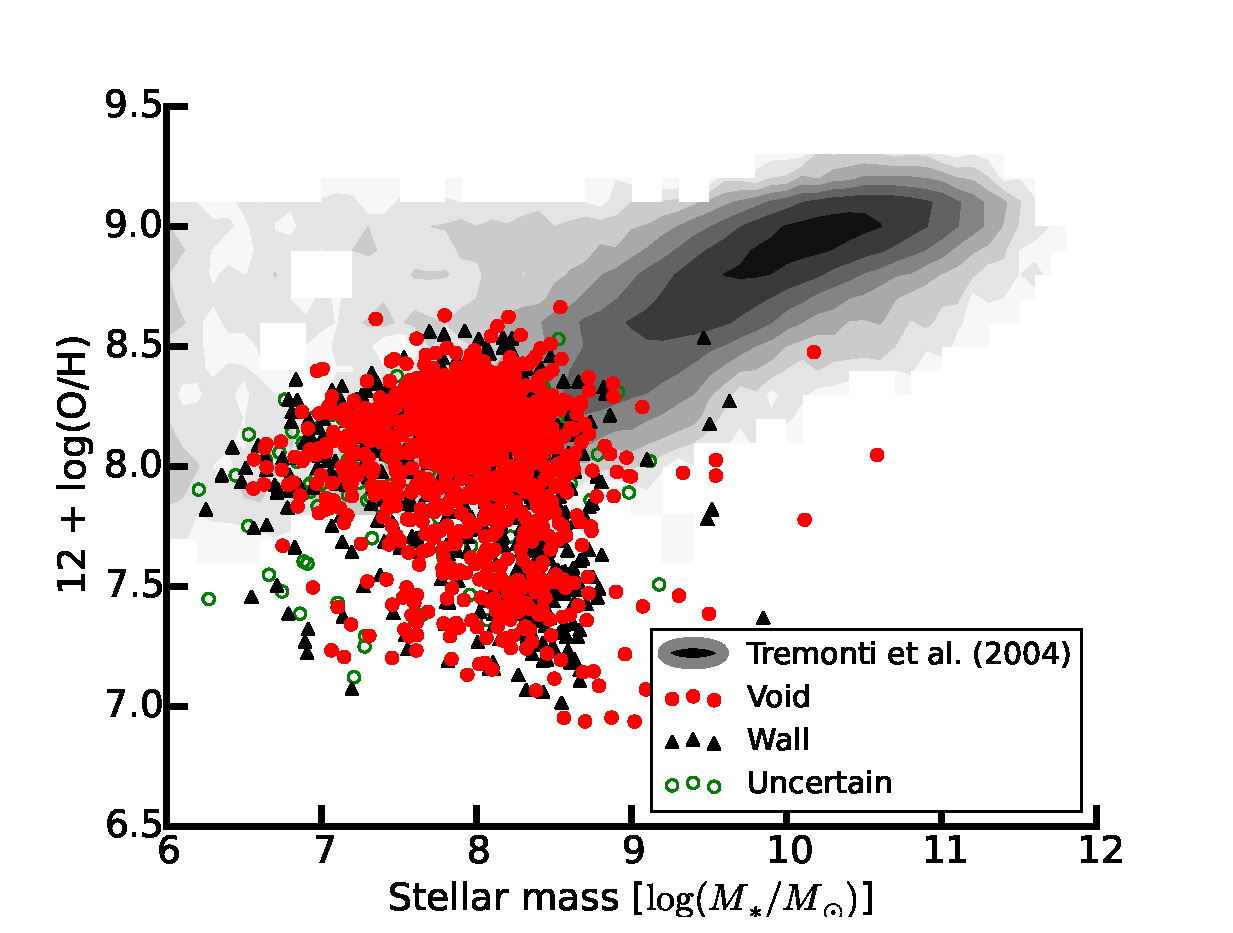
\includegraphics[width=0.49\textwidth]{Images/Paper3/MZ_1sig_I06relations_dwarf_SF_t3_dust_NSA_python}
    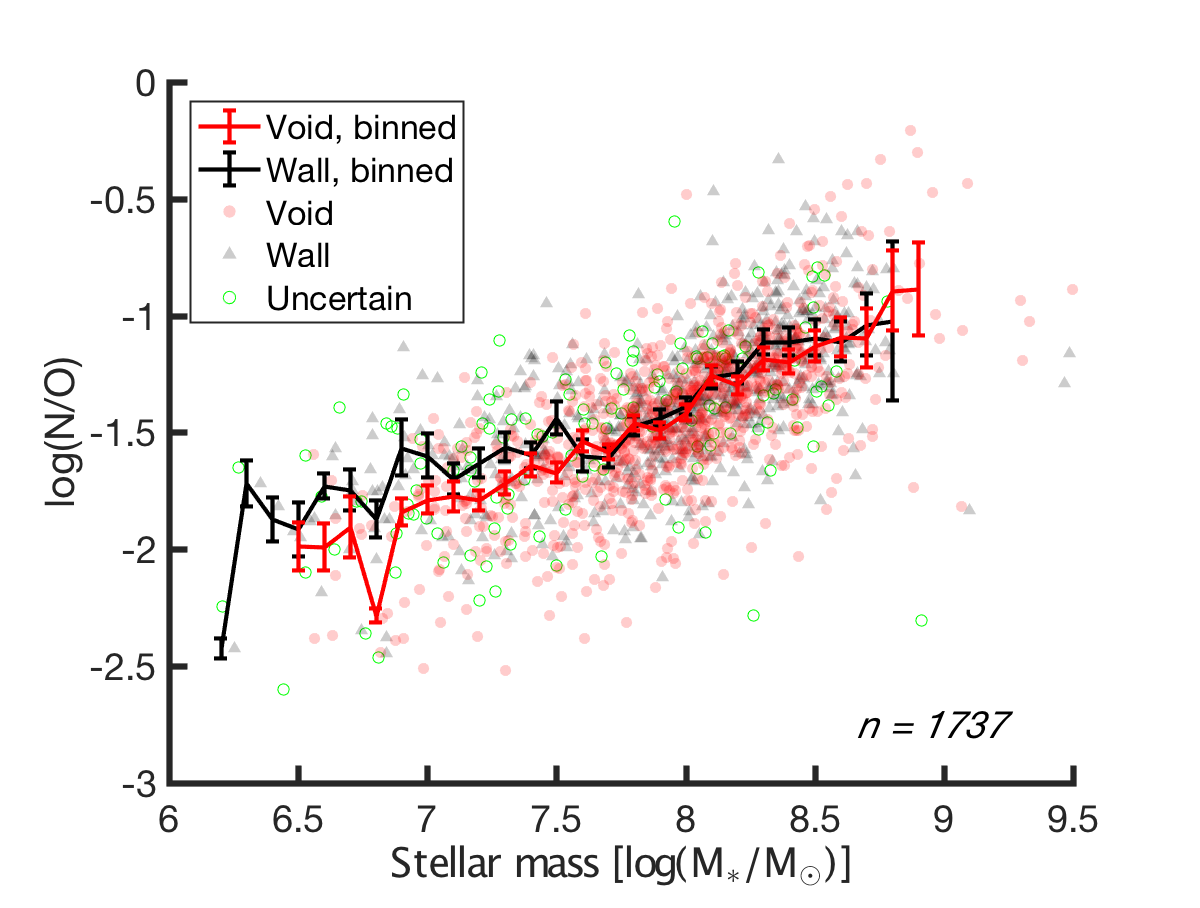
\includegraphics[width=0.49\textwidth]{Images/Paper3/MNO_1sig_I06relations_dwarf_SF_t3_dust_NSA_scatterMbin}
    \caption[$M_*$ versus N/O for star-forming dwarf galaxies]{Stellar mass 
    versus oxygen abundance (left panel) and N/O ratio (right panel).  We 
    include the metallicity results of \cite{Tremonti04} on the left to place 
    our dwarf galaxy abundance results in context.  On the right, we show the 
    average N/O values for the dwarf galaxies binned by stellar mass plotted 
    over the individual galaxies.  While most of our dwarf galaxies follow the 
    same trend as already seen in \cite{Tremonti04}, we note the existence of a 
    number of dwarf galaxies with much lower oxygen abundance values than what 
    would be predicted based on their stellar mass and the mass-metallicity 
    relation.  There is no clear difference between void and wall dwarf galaxies 
    in the mass-metallicity relation.  In the right-hand panel, though, we see 
    that the turn-off for the N/O plateau occurs at different masses for the two 
    large-scale environments.}
    \label{fig:M_NO}
\end{figure*}

Expanding on the mass-metallicity relation investigated in \cite{Douglass17a}, 
we look at the correlation between stellar mass and the oxygen abundance in our 
now substantially-larger sample of dwarf galaxies.  The mass-metallicity 
relation for our dwarf galaxies can be seen in Fig. \ref{fig:M_NO}.  We also 
include those galaxies from the MPA-JHU catalog with metallicity estimates from 
\cite{Tremonti04} to place our sample in context.  While most of our dwarf 
galaxies follow the same trend seen in \cite{Tremonti04}, we note the existence 
of a number of dwarf galaxies with much lower oxygen abundances than what would 
be predicted based on their stellar mass and the mass-metallicity relation.  
There is no discernible influence from the large-scale environment on the 
mass-metallicity relation for dwarf galaxies.

We also look at the N/O ratio as a function of stellar mass (Fig. 
\ref{fig:M_NO}, right panel).  Similar to the O/H--N/O relation studied in Sec. 
\ref{sec:NO_OH}, the N/O ratio is predicted to be constant below some critical 
mass; above this, the N/O ratio should increase linearly with the stellar mass.  
Unlike the relation seen in Fig. \ref{fig:NOvOH}, we see both the N/O plateau 
and the positive correlation on the right in Fig. \ref{fig:M_NO}.  To make the 
plot more readable, we also bin the galaxies by stellar mass in bins of width 
0.1.  We observe a difference in this relation as a function of the large-scale 
environment: the critical mass for void galaxies is around 
$\log(M_*/M_\odot) \sim$7.2, while the galaxies in denser regions exhibit a 
critical mass of $\sim$7.6.  This difference suggests that void galaxies begin 
to synthesize secondary nitrogen at lower stellar masses than galaxies in more 
dense regions, consistent with the results from Fig. \ref{fig:met1sig_P3} where 
void dwarf galaxies have higher oxygen abundances than dwarf galaxies in more 
dense environments.


%-------------------------------------------------------------------------------
\subsection{\ion{H}{1} mass-abundance relations}

\begin{figure*}
    \centering
    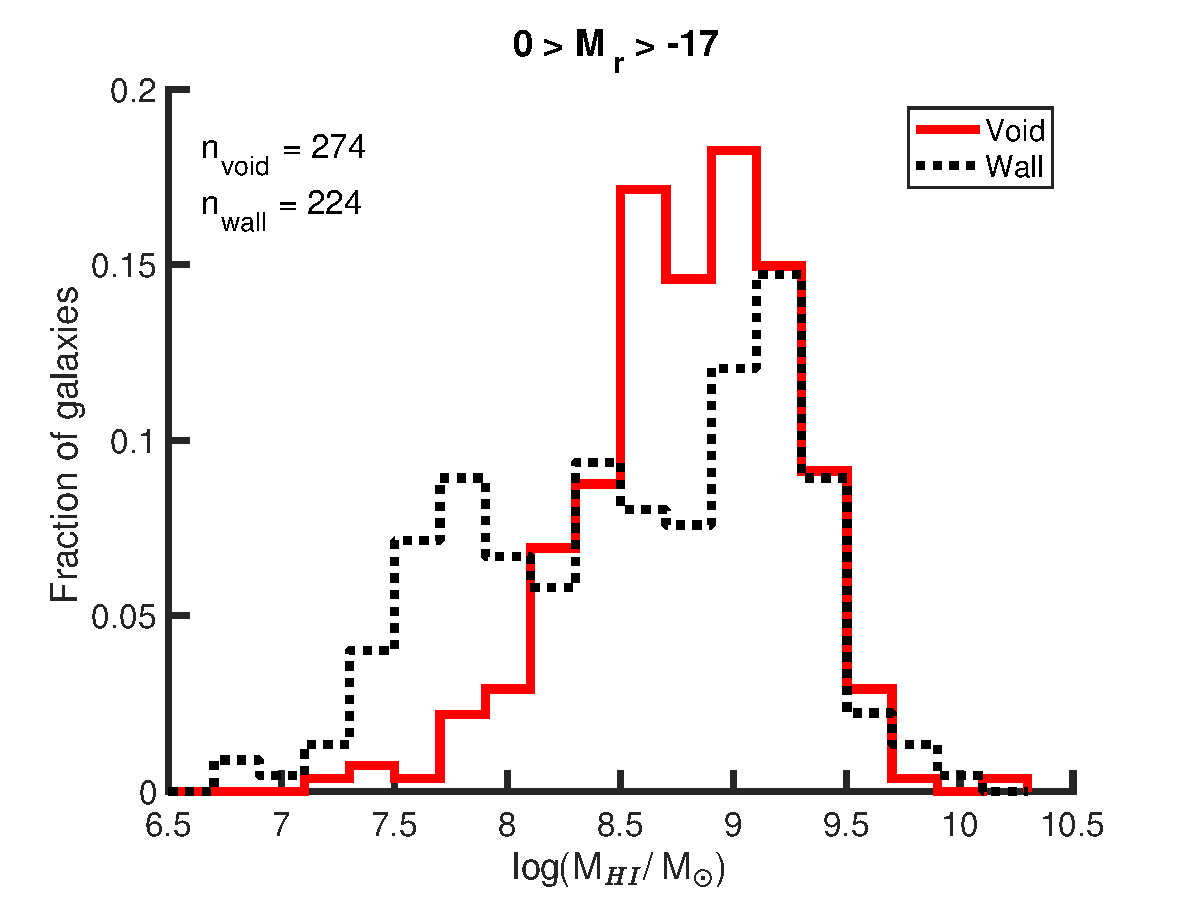
\includegraphics[width=0.49\textwidth]{Images/Paper3/1sig_0-17_I06relations_SF_t3_HI_hist}
    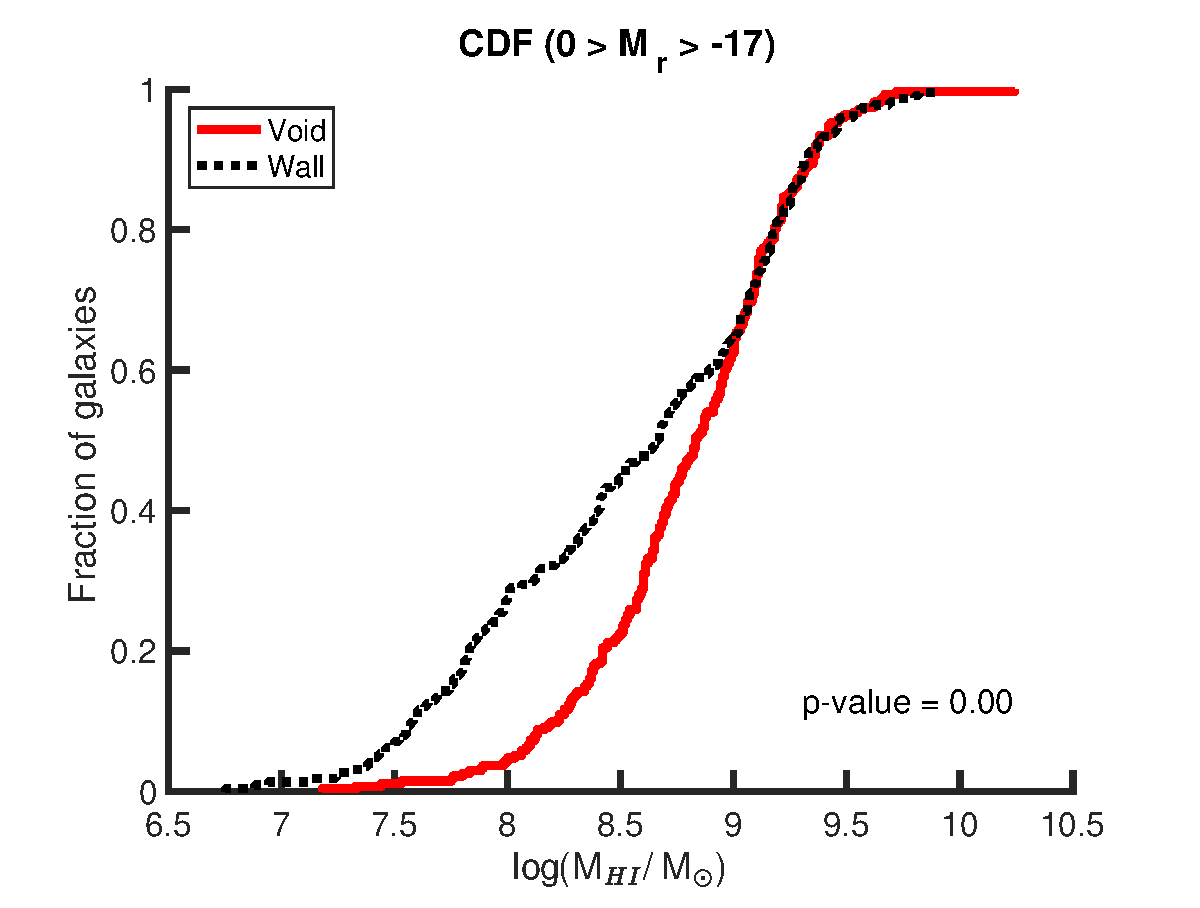
\includegraphics[width=0.49\textwidth]{Images/Paper3/1sig_0-17_I06relations_SF_t3_HI_CDF}
    \caption[\ion{H}{1} mass distribution]{The distribution of \ion{H}{1} mass 
    in the sample of dwarf galaxies, separated by their large-scale environment.  
    There is an obvious shift towards higher \ion{H}{1} masses in the void dwarf 
    galaxies.}
    \label{fig:HI_hist}
\end{figure*}

In addition to looking at the stellar mass, we also investigate the relationship 
between the amount of neutral hydrogen and the gas-phase chemical abundances in 
our sample of star-forming dwarf galaxies.  As shown in \cite{Moorman14}, void 
galaxies typically have lower \ion{H}{1} masses than galaxies in more dense 
regions, consistent with the overall shift of the luminosity or stellar mass 
function to lower luminosity or mass in voids.  In the fixed range of luminosity 
of our dwarf galaxy sample, as Fig. \ref{fig:HI_hist} shows, our sample of void 
dwarf galaxies have higher \ion{H}{1} masses than the dwarf galaxies in denser 
regions.  The gas in the void environment is cooler than that found in denser 
regions (due to less events like shock heating, etc.), which permits void 
galaxies to have higher \ion{H}{1} masses for a given stellar mass.  Therefore, 
because we are fixing the stellar mass in our sample of galaxies (by only 
studying dwarf galaxies), we should find that the void dwarf galaxies have 
higher \ion{H}{1} masses than for those dwarf galaxies in denser environments.

\begin{figure*}
    \centering
    \includegraphics[width=0.49\textwidth]{Images/Paper3/HI_OH_1sig_I06relations_dwarf+T04_SF_t3_dust}
    \includegraphics[width=0.49\textwidth]{Images/Paper3/HI_NO_1sig_I06relations_dwarf_SF_t3_dust}
    \includegraphics[width=0.49\textwidth]{Images/Paper3/HI_OH_M_1sig_I06relations_dwarf_SF_t3_dust}
    \includegraphics[width=0.49\textwidth]{Images/Paper3/HI_NO_M_1sig_I06relations_dwarf_SF_t3_dust}
    \caption[\ion{H}{1} mass versus O/H and N/O]{\ion{H}{1} mass versus 
    metallicity (left) and N/O ratio (right) for star-forming dwarf galaxies.  
    The color scheme of the top row emphasizes the large-scale environment of 
    the star-forming dwarf galaxies, while the bottom row investigates the 
    relationship between stellar mass, \ion{H}{1} mass, and chemical abundance.  
    Error bars have been omitted for clarity.  To place our oxygen abundance 
    results in context, we show (gray stars) the dwarf galaxies in SDSS DR7 with 
    metallicity estimates from \cite{Tremonti04}.  From these plots, there is no 
    significant influence from the large-scale environment on the relationship 
    between the \ion{H}{1} mass and gas-phase chemical abundances of 
    star-forming dwarf galaxies.}
    \label{fig:HI}
\end{figure*}

The \ion{H}{1} mass-metallicity and \ion{H}{1} mass-N/O relations can be seen in 
Fig. \ref{fig:HI}, extending the results of \cite{Bothwell13} down to 
$\log(M_*/M_\odot) \approx 6$.  Unlike the correlation between the stellar mass 
and the chemical abundances, there is very little correlation between the 
abundances and the \ion{H}{1} mass.  There is no significant relationship 
between the \ion{H}{1} mass and the metallicity of a galaxy --- a linear fit to 
the data in the left panel of Fig. \ref{fig:HI} reveals a slope of only 
$0.05\pm 0.085$ for the void population and $-0.04\pm 0.060$ for the wall 
population.  This is not surprising, as our sample of star-forming dwarf 
galaxies probes the low metallicity range of the MZ relation where there is no 
strong relationship between the metallicity and stellar mass.  There is a very 
small, but statistically significant, relationship between the \ion{H}{1} mass 
and the N/O ratio for the dwarf galaxies: a linear fit to the data in the right 
panel of Fig. \ref{fig:HI} reveals a slope of $0.11\pm 0.083$ for the void dwarf 
galaxies and $0.09\pm 0.060$ for the wall dwarf galaxies.

Due to the time delay in the production of nitrogen relative to oxygen, we 
expect the N/O ratio to decrease with increasing \ion{H}{1} mass, since more 
evolved galaxies have higher N/O ratios and will have used up most of their 
neutral hydrogen.  \cite{Bothwell13} demonstrates the existence of this 
relationship at a fixed stellar mass.  The first row of Fig. \ref{fig:HI} shows 
little, if any, relationship between the \ion{H}{1} mass and the chemical 
abundances.  However, the bottom row of Fig. \ref{fig:HI} shows that there is an 
inverse relationship between the chemical abundance and the \ion{H}{1} mass for 
fixed stellar mass (indicated by the colors of the points).


%-------------------------------------------------------------------------------
\subsection{Color-abundance relations}

\begin{figure*}
    \centering
    \includegraphics[width=0.49\textwidth]{Images/Paper3/ur_OH_1sig_I06relations_dwarf+T04_SF_t3_dust}
    \includegraphics[width=0.49\textwidth]{Images/Paper3/ur_NO_1sig_I06relations_dwarf_SF_t3_dust_scatterURbin}
    \caption[$u-r$ versus O/H and N/O for star-forming dwarf galaxies]{Color 
    ($u-r$) versus the gas-phase oxygen abundance (left) and the N/O ratio 
    (right) for star-forming dwarf galaxies.  Error bars on individual points 
    have been omitted for clarity.  For reference, the dwarf galaxies in SDSS 
    DR7 that have estimated metallicities from \cite{Tremonti04} are shown in 
    the left panel in gray.  To discern any environmental trends in the results, 
    we have binned the galaxies by their color (in bins of width 0.1) on the 
    right.  The large-scale environment does not influence the relationship 
    between the color and chemical abundances of dwarf galaxies.}
    \label{fig:ur_P3}
\end{figure*}

The gas-phase chemical abundance is expected to have a positive correlation with 
a galaxy's color.  Older galaxies have had more time to convert their gas into 
heavier elements through star formation, increasing their metallicities.  The 
color-metallicity and color-N/O relations for our sample of star-forming dwarf 
galaxies can be seen in Figures \ref{fig:ur_P3} and \ref{fig:gr}.  As we see, 
bluer galaxies have lower O/H and N/O ratios when we look at both the $u-r$ and 
$g-r$ colors.  While there is a subset of dwarf galaxies with extremely low 
metallicities that do not follow this trend (seen in the left-hand panels of 
Figures \ref{fig:ur_P3} and \ref{fig:gr}), this population follows the color-N/O 
trend seen on the right in each of these figures.  While these galaxies have 
unusually low oxygen abundances, they have normal N/O ratios.

\begin{figure*}
    \centering
    \includegraphics[width=0.49\textwidth]{Images/Paper3/gr_OH_1sig_I06relations_dwarf+T04_SF_t3_dust}
    \includegraphics[width=0.49\textwidth]{Images/Paper3/gr_NO_1sig_I06relations_dwarf_SF_t3_dust_scatterGRbin}
    \caption[$g-r$ versus O/H and N/O for star-forming dwarf galaxies]{Color 
    ($g-r$) versus the gas-phase oxygen abundance (left) and the N/O ratio 
    (right) for star-forming dwarf galaxies.  Error bars on individual points 
    have been omitted for clarity.  For reference, the galaxies in SDSS DR7 that 
    have estimated metallicities from \cite{Tremonti04} are shown in the left 
    panel in gray.  To discern any environmental trends in the results, we have 
    binned the galaxies by their color (in bins of width 0.1) on the right.  The 
    large-scale environment does not influence the relationship between the 
    color and chemical abundances of dwarf galaxies.}
    \label{fig:gr}
\end{figure*}

The presence of a relationship between the N/O ratio and the color of a galaxy 
can indicate a time delay between the release of nitrogen and oxygen 
\citep{vanZee06a,Berg12}.  If higher-mass stars are the main source of oxygen, 
then the oxygen will be released on a shorter time scale than nitrogen for a 
given star formation episode (since higher-mass stars turn off the main sequence 
earlier than the intermediate-mass stars that synthesize nitrogen).  Therefore, 
the amount of nitrogen relative to oxygen should increase as the hotter, more 
massive stars burn out and the galaxy becomes redder.  This trend can be seen in 
the star-forming dwarf galaxies on the right of Figures \ref{fig:ur_P3} and 
\ref{fig:gr}, matching the trends seen in \cite{Douglass17b,vanZee06a,Berg12}.

There does not appear to be any influence from the large-scale environment on 
the relationship between the color and chemical abundances for star-forming 
dwarf galaxies.  There is no obvious difference between the void and wall dwarf 
galaxies in the left-hand panels of Figures \ref{fig:ur_P3} and \ref{fig:gr}, 
when we concentrate on the oxygen abundance as a function of color.  To help 
discern any influence from the environment on the N/O ratio as a function of 
color, we bin the star-forming dwarf galaxies by their color in bins of width 
0.1 --- these results are overlaid on the left-hand plots of Figures 
\ref{fig:ur_P3} and \ref{fig:gr}.  The shift toward higher N/O ratios seen in 
the wall bins in both figures is the same shift identified in the histograms in 
Fig. \ref{fig:NOratio_P3}.  Any variation in the color-abundance relationship 
between the void and wall populations except a vertical shift would be evidence 
of the large-scale environment influencing the relationship.  There is a modest 
difference in the slope of these bins in N/O, where the colors of star-forming 
void dwarf galaxies are more strongly correlated with their N/O ratios than 
star-forming wall dwarf galaxies.  The Pearson correlation coefficient between 
$u-r$ and $\log (\text{N}/\text{O})$ for the star-forming void dwarf galaxies is 
$0.63\pm 0.019$ and $0.52\pm 0.027$ for the star-forming wall dwarf galaxies.  
The correlation coefficients between $g-r$ and $\log (\text{N}/\text{O})$ for 
the void dwarf galaxies is $0.74\pm 0.014$ and $0.67\pm 0.020$ for the wall 
dwarf galaxies.  
% What does it mean, for void galaxies to more correlated in their color v. N/O?


%-------------------------------------------------------------------------------
\subsection{(s)SFR-abundance relations}

\begin{figure*}
    \centering
    \includegraphics[width=0.49\textwidth]{Images/Paper3/SFR_OH_1sig_I06relations_dwarf+T04_SF_t3_dust}
    \includegraphics[width=0.49\textwidth]{Images/Paper3/SFR_NO_1sig_I06relations_dwarf_SF_t3_dust_scatterSFRbin}
    \caption[SFR versus O/H and N/O for star-forming dwarf galaxies]{SFR versus 
    metallicity (left) and the N/O ratio (right) for star-forming dwarf 
    galaxies.  Error bars for individual galaxies have been omitted for clarity.  
    To place our oxygen abundance results in context, we show (gray stars) the 
    dwarf galaxies in SDSS DR7 with metallicity estimates from 
    \cite{Tremonti04}.  To discern any environmental effects on the relation 
    between SFR and the N/O ratio, we bin the dwarf galaxies by SFR (in bins of 
    width 0.1).  From these plots, the large-scale environment has no 
    discernible influence on the relationship between the SFR and gas-phase 
    chemical abundances of star-forming dwarf galaxies.}
    \label{fig:SFR}
\end{figure*}

\begin{figure*}
    \centering
    \includegraphics[width=0.49\textwidth]{Images/Paper3/sSFR_OH_1sig_I06relations_dwarf+T04_SF_t3_dust}
    \includegraphics[width=0.49\textwidth]{Images/Paper3/sSFR_NO_1sig_I06relations_dwarf_SF_t3_dust_scattersSFRbin}
    \caption[sSFR versus O/H and N/O for star-forming dwarf galaxies]{Specific 
    star formation rate (sSFR) versus metallicity (left) and the N/O ratio 
    (right) for star-forming dwarf galaxies.  Error bars on individual galaxies 
    have been omitted for clarity.  To place our oxygen abundance results in 
    context, we show (gray stars) the dwarf galaxies in SDSS DR7 with 
    metallicity estimates from \cite{Tremonti04}.  To discern any environmental 
    effects on the relation between sSFR and the N/O ratio, we bin the dwarf 
    galaxies by sSFR (in bins of width 0.1).  From these figures, there is no 
    significant influence on the relationship between the sSFR and gas-phase 
    chemical abundances of star-forming dwarf galaxies.}
    \label{fig:sSFR_P3}
\end{figure*}

There is thought to be a fundamental relationship between the stellar mass, star 
formation rate (SFR), and metallicity of a galaxy \citep{Mannucci10,LaraLopez10,
Andrews13}; the metallicity of a galaxy should increase with stellar mass and 
decrease as a function of the SFR.  \cite{Henry13} observe an inverse 
relationship between the metallicity and SFR of low-mass galaxies.  However, as 
was seen in \cite{Douglass17a}, Fig. \ref{fig:SFR} shows very little correlation 
between the SFR and metallicity or N/O ratio of the star-forming dwarf galaxies.  
When we separate the dwarf galaxies by their large-scale environment, we see no 
difference in the correlation coefficients between the two environments; there 
is no discernible influence on the relationship between the SFR and the chemical 
abundances by the large-scale environment.

We also inspect the relationship between the specific star formation rate (sSFR) 
and the gas-phase chemical abundances in star-forming dwarf galaxies.  As shown 
in Fig. \ref{fig:sSFR_P3}, there is a stronger correlation between the sSFR of a 
dwarf galaxy and its metallicity and N/O ratio.  The left-hand panel of Fig. 
\ref{fig:sSFR_P3} shows the relationship between the gas-phase oxygen abundance 
and the sSFR for star-forming dwarf galaxies; to place our results in context, 
we also include (gray stars) those dwarf galaxies in SDSS DR7 for which 
\cite{Tremonti04} was able to estimate metallicities.  In the metallicity regime 
we are able to probe (\OH $\leq 8.5$), the star-forming dwarf galaxies display 
relatively little relationship between their sSFR and metallicity.  The group of 
extremely low metallicity dwarf galaxies (\OH $< 7.6$) in our sample has some of 
the lowest sSFR of our dwarf galaxies.

As we see on the right in Fig. \ref{fig:sSFR_P3}, though, there is a strong 
anti-correlation between the sSFR and N/O ratio for the star-forming dwarf 
galaxies.  Galaxies with higher sSFRs may be producing more massive stars than 
galaxies with lower sSFRs.  If oxygen is produced in more massive stars than 
those which produce nitrogen, then the galaxies with higher sSFRs will produce 
more oxygen earlier than those galaxies with lower sSFRs.  Increasing the 
gas-phase oxygen abundance relative to nitrogen will decrease the N/O ratio in 
these galaxies with higher sSFRs.  Therefore, an anti-correlation between the 
sSFR and N/O ratio is further evidence that oxygen is produced in higher mass 
stars than those which synthesize nitrogen.

There is also very little scatter in the right-hand panel of Fig. 
\ref{fig:sSFR_P3}, indicating a significant relationship between the sSFR and 
N/O ratio for dwarf galaxies.  The Pearson correlation coefficients for our 
sample of star-forming void dwarf galaxies is $-0.62\pm 0.020$; the correlation 
coefficient for the star-forming wall dwarf galaxies is $-0.55\pm 0.025$.  It is 
interesting to note that the void dwarf galaxies exhibit a stronger correlation 
between their sSFR and N/O ratio than the dwarf galaxies in denser environments.  
This can be seen in the binned data points plotted on top of the individual 
dwarf galaxies; we have taken the average of the galaxies binned by their sSFR 
(in bins of width 0.1) to help discern any large-scale environmental influence 
on the relationship between the sSFR and the N/O ratio.
% Again, what is the physical interpretation of the stronger correlation in the void galaxies?



%%%%%%%%%%%%%%%%%%%%%%%%%%%%%%%%%%%%%%%%%%%%%%%%%%%%%%%%%%%%%%%%%%%%%%%%%%%%%%%%
%
%    DISCUSSION
%
%%%%%%%%%%%%%%%%%%%%%%%%%%%%%%%%%%%%%%%%%%%%%%%%%%%%%%%%%%%%%%%%%%%%%%%%%%%%%%%%
\section[Environmental influence]{Large-scale environmental influence}

We see small, statistically significant shifts in each of the three gas-phase 
abundance ratios studied as a function of the large-scale environment, implying 
that the large-scale environment influences the chemical abundances of 
star-forming dwarf galaxies.  Previous work by \cite{Douglass17b} suggests that 
the oxygen abundance (O/H), nitrogen abundance (N/H), and N/O ratio depend on a 
galaxy's environment.  Work by \cite{Shields91} finds no shift in the N/O ratio 
between cluster and field galaxies, though they do find that cluster galaxies 
have higher metallicities than field galaxies.  \cite{Contini02} and 
\cite{Pilyugin02} find a statistically insignificant shift in the N/O ratio 
between cluster and field galaxies, where cluster galaxies have lower N/O ratios 
than field spiral galaxies.  The shifts seen in each of these latter three 
sources are opposite to what we observe in this paper, though these previous 
studies concentrate on the galaxies in the Virgo cluster, which are more massive 
than our dwarf galaxy ($M_r > -17$) sample.  On average, we find that 
star-forming void dwarf galaxies have $\sim$7\% higher oxygen abundances, 
$\sim$10\% lower nitrogen abundances, and $\sim$17\% lower N/O ratios than 
star-forming dwarf galaxies in denser regions.

As outlined in \cite{Douglass17a}, there have been numerous previous studies 
that investigate the influence of the environment on the metallicity of a 
galaxy, resulting in mixed conclusions.  When a difference in the metallicity 
was attributed to the environment \citep[as in][for example]{Pustilnik06,
Pustilnik11b,Pustilnik14,SanchezAlmeida16,Cooper08}, it was found that those 
galaxies with higher metallicities preferentially reside in denser regions.  
This is the opposite of the trend seen in Fig. \ref{fig:met1sig_P3} in the 
star-forming dwarf galaxies, although our results are not a direct comparison 
with their conclusions (do to our requirement of the [\ion{O}{3}] $\lambda$4363 
auroral line, we are not able to probe the high-metallicity regime).  We observe 
an average metallicity that is $\sim$7\% higher in void dwarf galaxies than in 
dwarf galaxies in denser regions.


\subsection{Higher metallicities in void dwarf galaxies}

% The direction of the shift implies more O in voids
%  - How do we get more O in void galaxies?  M_DM/M_* |v > M_DM/M_* |w
We posit that the slightly higher metallicities seen in the star-forming void 
dwarf galaxies in Fig. \ref{fig:met1sig_P3} is due to a large-scale 
environmental effect on the ratio of a galaxy's dark matter halo mass to stellar 
mass ($M_{DM}/M_*$).  \cite{Goldberg04} show that gravitational clustering 
within a void proceeds as if in a very low density universe, where the growth of 
gravitationally bound dark matter halos ends relatively early.  Afterwards, 
there is relatively little interaction between the void galaxies because of the 
lower density and faster local Hubble expansion.  Simulations by \cite{Jung14} 
and \cite{Tonnesen15} show that, for a fixed dark matter halo mass, the stellar 
masses of central galaxies located in voids are smaller than those of central 
galaxies living in denser regions.  The $\Lambda$CDM cosmology predicts that 
galaxies formed in voids will be retarded in their star formation when compared 
to those in denser environments.  Therefore, void dwarf galaxies could have 
higher $M_{DM}/M_*$ ratios than dwarf galaxies in denser regions.

If this is the case, then the potential well and virial radius of the void 
galaxies are large enough to retain more of the heavy elements that are blown 
from the ISM to the CGM of a galaxy (from a supernova, for example).  The 
simulation results of \cite{Tonnesen15} find that, for central galaxies with 
halo masses between $10^{11}$ and $10^{12.9}$, void galaxies have $\sim$10\% 
larger ratios of dark matter halo mass to stellar mass than wall galaxies at 
$z = 0$.  In wall galaxies, more of these heavy elements can escape the dwarf 
galaxy, while in void galaxies they are confined to the CGM and eventually fall 
back onto the galaxy's ISM.  If star-forming void dwarf galaxies are able to 
retain more oxygen relative to their hydrogen abundance, then they will reach 
the critical value of O/H for secondary nitrogen production (via the CNO cycle) 
earlier than the star-forming wall dwarf galaxies, for a given stellar mass.  We 
see this in Fig. \ref{fig:M_NO}, where the N/O plateau for the void dwarf 
galaxies exists for stellar masses $\log(M_*/M_\odot) \lesssim 7.2$.  In 
contrast, the N/O plateau for the wall dwarf galaxies exists for stellar masses 
$\log(M_*/M_\odot) \lesssim 7.6$.

% What other proof do we have that this might be true?
If void dwarf galaxies have higher $M_{DM}/M_*$ ratios than dwarf galaxies in 
denser environments, we would expect to see an environmental influence on other 
characteristics of these galaxies.  First, the ratio of neutral hydrogen mass to 
stellar mass of the dwarf galaxies would be higher in star-forming void galaxies 
than star-forming wall galaxies, under the assumption that neutral hydrogen 
traces dark matter.  We see this effect both in Fig. 9 of \cite{Moorman16} and 
in Fig. \ref{fig:HI_hist} above.  Second, the \ion{H}{1} mass function should 
shift less from wall to void galaxies than the shift seen in the luminosity 
function.  Indeed, \cite{Moorman16} finds a shift of characteristic \ion{H}{1} 
mass by a factor of 1.4 in the \ion{H}{1} mass function, while \cite{Hoyle05} 
measures a shift by a factor of 2.5 in luminosity in the luminosity function 
between these two environments.


\subsection{Lower N/O ratios in void dwarf galaxies}

% Shift in N/O due to environmental influence on cosmic downsizing
As we see in Fig. \ref{fig:NOratio_P3}, star-forming void dwarf galaxies have a 
lower N/O ratio than wall dwarf galaxies.  This strengthens the preliminary 
results found in \cite{Douglass17b} and the simulation results of \cite{Cen11}, 
indicating that void galaxies are retarded in their star formation and that 
cosmic downsizing might depend on the large-scale environment.  As suggested by 
\cite{vanZee06a}, a galaxy with a declining SFR at late times (a wall galaxy) 
will have a higher N/O ratio than a galaxy with a constant SFR (a void galaxy); 
the ongoing star formation in the void galaxies will release more oxygen into 
the ISM, decreasing their N/O ratio relative to the galaxies with declining 
SFRs.  This concept is supported by the color-N/O diagram in Figures 
\ref{fig:ur_P3} and \ref{fig:gr}, where the bluer galaxies have lower N/O 
ratios.  The correlations between color and the N/O ratio found in 
\cite{vanZee06a}, \cite{Berg12}, \cite{Douglass17b}, and this work are a result 
of declining SFRs \citep{vanZee06a}.  The average lower N/O ratios we see in 
star-forming void dwarf galaxies may be observational evidence that cosmic 
downsizing is environmentally dependent.


\subsection{Extremely low metallicity dwarf galaxies}

Previous studies have either hypothesized \citep{Pustilnik06,Pustilnik11b,
Pustilnik13} or concluded \citep{Filho15} that low-metallicity objects 
preferentially reside in low-density environments.  \cite{Douglass17a} find 
that, out of 135 dwarf galaxies studied, there is no difference in the fraction 
of low-metallicity dwarf galaxies that reside in voids and denser regions.  Of 
the 1920 dwarf galaxies we analyze, 287 have extremely low metallicity values 
(\OH $\leq 7.6$).  Of these 287 low-metallicity dwarf galaxies, 144 are found in 
voids (approximately 15\% of the star-forming void dwarf galaxy population 
studied) and 122 are located in denser regions (16\% of the star-forming wall 
dwarf galaxy population studied).  These population fractions do not support the 
existence of a special population of extremely metal-poor dwarf galaxies in 
voids.

We find that these 287 extremely metal-poor galaxies are only slightly lower in 
their nitrogen abundances when compared to the total star-forming dwarf galaxy 
population studied.  The low oxygen abundances causes these dwarf galaxies to 
have higher N/O ratios than the total star-forming dwarf galaxy population 
studied.  From Figures \ref{fig:ur_P3} and \ref{fig:gr}, it is apparent that 
these extremely metal-poor star-forming dwarf galaxies are redder than their 
oxygen abundances would typically indicate, although their colors align with 
their N/O ratios.  Fig. \ref{fig:SFR} also shows that the sSFRs for these 
low-metallicity dwarf galaxies are lower than expected for their oxygen 
abundances, though their sSFRs conform with the observed relationship between 
the N/O ratio and the sSFR.  The 287 extremely metal-poor galaxies are isolated 
from our main sample of star-forming dwarf galaxies only when comparing their 
gas-phase oxygen abundances to other physical characteristics; their N/O ratios 
are not unusual.


%%%%%%%%%%%%%%%%%%%%%%%%%%%%%%%%%%%%%%%%%%%%%%%%%%%%%%%%%%%%%%%%%%%%%%%%%%%%%%%%
%
%    CONCLUSION
%
%%%%%%%%%%%%%%%%%%%%%%%%%%%%%%%%%%%%%%%%%%%%%%%%%%%%%%%%%%%%%%%%%%%%%%%%%%%%%%%%
\section{Conclusions}

% Need a topic sentence that refers back to the introduction
We estimate the gas-phase oxygen and nitrogen abundances and the N/O ratio of 
star-forming dwarf galaxies in SDSS DR7 using the direct $T_e$ method and 
spectroscopic line flux measurements as reprocessed in the MPA-JHU catalog.  We 
expand upon the previous work of \cite{Douglass17a} and \cite{Douglass17b} by 
deriving a relation between the doubly-ionized oxygen and total oxygen abundance 
in star-forming galaxies; removing the dependence on the [\ion{O}{3}] 
$\lambda$3727 doublet, this relation allows us to probe those dwarf galaxies at 
$z < 0.02$ in SDSS DR7.  The 1920 dwarf galaxies analyzed indicate that the 
large-scale environment influences their chemical evolution: star-forming void 
dwarf galaxies have higher oxygen abundances by an average of 7\%, lower 
nitrogen abundances by an average of 10\%, and 17\% lower N/O ratios than 
star-forming dwarf galaxies in denser regions.  The large-scale ($\sim$10 \hMpc) 
environment influences the chemical evolution of star-forming dwarf galaxies.

% Summary of comparison with physical characteristics
In addition, we also look at the relationship between the metallicity and the 
N/O ratio and other physical characteristics of our star-forming dwarf galaxy 
sample.  In the relationship between N/O and O/H, all our dwarf galaxies reside 
on the so-called ``nitrogen plateau,'' where the N/O ratio is predicted to be 
independent of the gas-phase oxygen abundance for metallicities \OH $< 8.5$.  
Instead of a constant value for the N/O ratio, we instead find that the N/O 
ratio decreases with increasing metallicity.  However, we do find a plateau in 
our relationship between the stellar mass and N/O ratio.  Most of our 
star-forming dwarf galaxies follow the typical mass-metallicity relation 
\citep{Tremonti04}.  There is no relationship between the metallicity and 
\ion{H}{1} mass of the galaxies, but the N/O ratio decreases with increasing 
\ion{H}{1} mass for fixed stellar mass.  The star-forming dwarf galaxies exhibit 
an increase in the metallicity (O/H) and N/O ratio with increasing color (both 
$u-r$ and $g-r$).  We see very little correlation with SFR for either 
metallicity (O/H) or N/O ratio of dwarf galaxies, but the metallicity and N/O 
ratio decrease with increasing sSFR.  Beyond the large-scale environmental 
influence on the chemical abundance distributions in the sample of star-forming 
dwarf galaxies, we do not observe any significant differences between the 
star-forming void and wall dwarf galaxies in any of these relationships.

% Physical interpretation for the shift in O/H, N/O
We surmise that the differences in the distributions of metallicity and the N/O 
ratio seen in the sample of star-forming dwarf galaxies are due to a large-scale 
environmental influence on their formation history and evolution.  The shift in 
the gas-phase oxygen abundance distribution could be observational evidence for 
delayed star formation in void galaxies when compared to those in denser 
regions.  This would result in a smaller ratio of stellar mass to dark matter 
halo mass in void galaxies than in wall dwarf galaxies, as predicted in 
simulations by \cite{Jung14} and \cite{Tonnesen15}.  Simulations looking at how 
the retention fraction of supernovae ejecta depends on the halo mass or dark 
matter potential would be useful in understanding if a $\sim$10\% increase in 
the dark matter halo mass for void dwarf galaxies is enough to result in a 
$\sim$7\% increase in the metallicity.  If the void galaxies are retaining more 
oxygen as a result of their deeper potential wells, then they will be able to 
commence the synthesis of secondary nitrogen earlier, as is seen in the mass-N/O 
relation in Fig. \ref{fig:M_NO}.  In addition, the shift towards lower N/O 
ratios in the star-forming void dwarf galaxies may be evidence that cosmological 
downsizing is environmentally dependent.  Our results provide evidence for 
delayed, ongoing star formation in void dwarf galaxies whose dark matter halos 
ceased coalescing earlier than for dwarf galaxies in denser regions.

% XMP dwarf galaxies
No special population of extremely metal-poor star-forming dwarf galaxies is 
found in the voids, as we note an equal fraction of low metallicity dwarf 
galaxies in both the voids and denser regions.  Due to their low gas-phase 
oxygen abundances, the 287 dwarf galaxies have some of the larger N/O ratios of 
the star-forming dwarf galaxy sample studied.  While the metallicities of these 
galaxies cause them to stand out when looking at the relationship between the 
metallicity and other physical characteristics of the galaxies (stellar mass, 
color, (s)SFR), they are not unusual when studying the relationship between the 
N/O ratio and the other galaxy properties.

% Chapter: Small-scale environment
\chapter[Small-Scale Environment]{The Influence of the Small-Scale Environment on Dwarf Galaxy Evolution}\label{ch:smallScaleEnvironment}


This work was done in collaboration with Daniele Schneider for her senior thesis 
``The effects of small-scale environment on dwarf galaxies.''


%%%%%%%%%%%%%%%%%%%%%%%%%%%%%%%%%%%%%%%%%%%%%%%%%%%%%%%%%%%%%%%%%%%%%%%%%%%%%%%%
%%%%%%%%%%%%%%%%%%%%%%%%%%%%%%%%%%%%%%%%%%%%%%%%%%%%%%%%%%%%%%%%%%%%%%%%%%%%%%%%


\section{Introduction}

%% Large-scale environment influence
%Large galaxy redshift surveys have shown that the large-scale structure of the 
%distribution of galaxies in the universe is similar to that of a 
%three-dimensional cosmic web \citep{Bond96}, where galaxy clusters are connected 
%by thin filaments of galaxies and are separated by voids (large, underdense 
%regions that occupy close to 60\% of space).  Over the last few decades, the 
%Sloan Digital Sky Survey \citep{Abazajian09,Ahn12} has accelerated the research 
%into the influence of the large-scale environment on the formation and evolution 
%of galaxies.
%
%Because gravitational clustering within a void proceeds as if in a very 
%low-density universe, cosmic voids are an important environment for studying 
%galaxy formation \citep[see][for a review]{vandeWeygaert11}.  The $\Lambda$CDM 
%cosmology predicts that galaxies formed in voids have lower masses and are 
%retarded in their star formation when compared to those in more dense 
%environments \citep{Gottlober03,Goldberg05,Cen11}.  The effects of the void 
%environment should be most obvious in dwarf galaxies due to their minimal 
%gravitational potential.  As a result, they are more sensitive to astrophysical 
%effects such as cosmological reionization, internal feedback from supernovae and 
%photoheating from star formation, small-scale details of dark matter halo 
%assembly, and the properties of dark matter.
%
%Observations have shown that the properties of dwarf galaxies vary dramatically 
%with the environment \citep[e.g.,][]{Ann08,Geha12}.  Void galaxies have been 
%found to have lower stellar mass \citep{Hoyle05,Croton05,Moorman15}, be bluer 
%and of a later type \citep{Grogin00,Rojas04,Patiri06,Park07,vonBendaBeckmann08,
%Hoyle12}, have higher star formation rates \citep{Rojas05,Moorman15,Beygu16}, 
%and be more gas rich \citep{Kreckel12,Moorman16,Jones16} than galaxies in denser 
%regions.

% Small-scale environment - what has been done so far?
In conjunction with the large-scale environment, the small-scale environment 
($\sim$1 \hMpc) has also been found to influence a galaxy's evolution.  A 
well-established morphology-density relation exists \citep{Dressler80}, where 
the fraction of late-type galaxies is inversely proportional to the local 
density.  \cite{Ellison09} determined that a galaxy's local environment 
influences a galaxy's evolution more than its large-scale environment.  
Likewise, \cite{Rupke08} concluded that interacting galaxies have suppressed 
metallicities, because interactions induce flows of hydrogen.  \cite{Park09} 
found that, for galaxies with $M_r < -19$, galaxy interactions out to the virial 
radius of the nearest neighbor influence the evolution of the target galaxy.  
Along with \cite{Park07}, they determine that the large-scale environment has a 
minimal effect on the evolution of a galaxy once the luminosity and morphology 
are taken into account.

We want to understand if the small-scale environment is more influential in a 
galaxy's evolution than its large-scale environment.  One important question 
within the small-scale environment asks if tidal influences due to the nearest 
neighbor galaxy or gravitational potentials from the nearest galaxy group are 
more influential in a galaxy's evolution.  A group consists of multiple galaxies 
that share the same dark matter halo.  A group member will interact 
gravitationally with all other group members, not just its nearest neighbor.  In 
groups and clusters dense enough to strip and heat the gas, galaxies will also 
experience ram pressure stripping.  And a galaxy near a group, but not within 
it, may also experience strong tidal effects from the group similar to and 
stronger than those from a neighboring galaxy.



%%%%%%%%%%%%%%%%%%%%%%%%%%%%%%%%%%%%%%%%%%%%%%%%%%%%%%%%%%%%%%%%%%%%%%%%%%%%%%%%
%%%%%%%%%%%%%%%%%%%%%%%%%%%%%%%%%%%%%%%%%%%%%%%%%%%%%%%%%%%%%%%%%%%%%%%%%%%%%%%%


\section[Nearest neighbor calculations]{Identifying the nearest neighbor}\label{sec:Theory_dist}

We employ two different spatial metrics to determine the best way to locate a 
galaxy's nearest neighbor.  We set a maximum velocity separation of 300 km/s 
between a galaxy and its nearest neighbor to capture the majority of interacting 
galaxies \citep[according to the distribution in peculiar velocity shown in][]
{Hwang10}.  Within a relative velocity $v_{rel} < 300\text{ km/s}$, we use 
either the physically closest galaxy in units of \hMpc or the galaxy within the 
smallest fraction of its virial radius; both these methods are described below 
in further detail.  The two methods result in different neighboring galaxies for 
about 40\% of our dwarf galaxy sample.


\subsection{Peculiar velocity}
% Finger of God

A galaxy's redshift is composed of both the expansion of the universe and the 
galaxy's peculiar velocity (its motion relative to its surrounding galaxies and 
environment).  Known as the ``Finger of God'' effect, the peculiar velocity 
causes galaxy groups and clusters to appear extended along the line of sight 
when using redshift as a distance measurement.  When we calculate distances on 
large scales, the peculiar velocity is negligible.  However, when we study the 
distance between two objects in the universe on a small scale (within a few 
\hMpc), the peculiar velocity dominates.  The relative velocity $v_{rel}$ 
between galaxies $a$ and $b$ is defined as
\begin{equation}
    v_{rel} = |z_a - z_b|c
\end{equation}
where $z$ is the redshift.  We require all 
neighbors to have a maximum relative velocity $v_{rel} < 300\text{ km/s}$, as we 
believe those outside this range will have minimal influence on the target 
galaxy's evolution.  We show in Sec. \ref{sec:selection_effects} that our 
results are insensitive to this value.


\subsection{Sky separation in \hMpc}

The projected distance between two galaxies is found by projecting the two 
galaxies onto a sphere of radius $\bar{r}$, where $\bar{r}$ is the average 
distance from Earth of the two galaxies.  This assumes that two galaxies which 
are gravitationally bound are in a system where the relative velocity between us 
and it is 0 and that $\bar{r}$ is the distance to the center of the system.  For 
redshifts $z \ll 1$, we can approximate the distance to the system is as
\begin{equation}
    \bar{r} = \frac{\bar{z}c}{H_0}
\end{equation}
where $\bar{z}$ is the average redshift of the two galaxies, $c$ is the speed of 
light, and $H_0$ is the Hubble constant.  Each galaxy's right ascension (RA) and 
declination (dec.) are converted to Cartesian coordinates to find their sky 
separation.


\subsection{Fractional virial radii}
% Virial radius calculation

The virial radius of a galaxy defines the region within which something is 
gravitationally bound to the galaxy.  From \cite{Hwang10}, we calculate the 
virial radius of a galaxy to be
\begin{equation}\label{eqn:r_vir}
    r_{vir} = (3L\gamma/4\pi/200\rho_c)^{1/3}
\end{equation}
where $L$ is the galaxy's luminosity, $\gamma$ is the mass-to-light ratio, and 
$\rho_c$ is the critical density of the universe.  The critical density is the 
density at which evenly distributed gas would collapse to form a galaxy.  

\cite{Choi07} find that the velocity dispersion of a galaxy depends on its 
morphological type, where $\sqrt{2}\sigma_{late} \approx \sigma_{early}$.  In 
terms of the velocity dispersion, the kinetic energy of a galaxy 
$K = 3/2 \sigma^2$.  Its gravitational potential energy $U = 3GM/5R$.  
Therefore, the virial theorem shows us that
\begin{align}
    3\sigma^2 \simeq \frac{3}{5} \frac{GM}{R}\nonumber \\
    M \simeq \frac{5\sigma^2 R}{G}
\end{align}
With $\gamma \equiv M/L$, at a fixed luminosity and virial radius we see that
\begin{equation}
    \gamma_{late} \simeq \frac{5\sigma_{late}^2 R}{GL} \qquad \gamma_{early} \simeq \frac{5\sigma_{early}^2 R}{GL}
\end{equation}
Taking the ratio of the two mass-to-light ratios and using the relation between 
the velocity dispersions found by \cite{Choi07}, we find that the mass-to-light 
ratio depends on the galaxy's morphology type: $\gamma_{early} = 2\gamma_{late}$.

\cite{Hwang10} defines $200\rho_c = 740\bar{\rho}$, where 
$\bar{\rho} = (0.0223\pm 0.0005)(\gamma_{late}L_{-20})(\text{\hMpc})^3$.  We can 
then rewrite Eqn. \ref{eqn:r_vir} as
\begin{equation}
    r_{vir} = \left( \frac{3}{4\times 740\times 0.0223\pi} \frac{\gamma}{\gamma_{late}} \frac{L}{L_{-20}} \right)^{1/3}
\end{equation}
where $L_{-20}$ is the luminosity of a galaxy with $M_r = -20$.  We can then use 
the virial radius to scale the distance between two galaxies as a fraction of 
the neighbor's virial radius.

Rather than using a measure of the virial radius for the group analysis, we 
scale the distance as a fraction of the group's root mean square (rms) radius.


\subsection{Absolute distance to nearest neighbor}
% Including redshift

We can also calculate the distance between two galaxies by ignoring the effects 
of their relative velocities.  Instead of projecting both galaxies onto a sphere 
with radius $\bar{r}$, we instead project each onto its own sphere of radius 
\begin{equation}
    r = \frac{cz}{H_0}
\end{equation}
(This approximation for the distance is valid because all our target galaxies 
are within a redshift $z \leq 0.03$.)  We then convert to Cartesian coordinates 
and use the three-dimensional Pythagorean theorem to calculate the distance 
between the two galaxies.


%%%%%%%%%%%%%%%%%%%%%%%%%%%%%%%%%%%%%%%%%%%%%%%%%%%%%%%%%%%%%%%%%%%%%%%%%%%%%%%%
%%%%%%%%%%%%%%%%%%%%%%%%%%%%%%%%%%%%%%%%%%%%%%%%%%%%%%%%%%%%%%%%%%%%%%%%%%%%%%%%


\section[SDSS Data]{SDSS Data and galaxy selection}

% SDSS
%The Sloan Digital Sky Survey Data Release 7 \citep[SDSS DR7;][]{Abazajian09} is 
%a wide-field multiband imaging and spectroscopic survey which maps approximately 
%one-quarter of the northern sky using a drift scanning technique.  Photometric 
%data in the five-band SDSS system --- $u$, $g$, $r$, $i$, and $z$ --- is taken 
%on a dedicated 2.5m telescope at the Apache Point Observatory in New Mexico 
%\citep{Fukugita96,Gunn98}.  Galaxies with Petrosian $r$-band magnitudes 
%$m_r < 17.77$ are selected for follow-up spectroscopic analysis \citep{Lupton01,
%Strauss02}.  The galaxy colors are taken from the Korean Institute for Advanced 
%Study Value-Added Galaxy Catalog \citep[KIAS-VAGC;][]{Choi10}, which contains 
%galaxies from the SDSS DR7 main sky survey based on the New York University 
%Value-Added Galaxy Catalog Data Release 7 \citep[NYU-VAGC;][]{Blanton05}.  Total 
%star formation rates (SFR) and total specific star formation rates (sSFR) are 
%from the MPA-JHU value-added catalog\footnote{Available at 
%\url{http://www.mpa-garching.mpg.de/SDSS/DR7/}}, calculated using the technique 
%described in \cite{Brinchmann04}.  
The gas-phase chemical abundances used are from Douglass, Vogeley, and Cen 
(2017, submitted), which are calculated using the Direct $T_e$ method.  The 
galaxies' large-scale environments are based on the void catalog compiled by 
\cite{Pan12}, which is constructed from SDSS DR7 using the VoidFinder algorithm 
of \cite{Hoyle02}.  Galaxies that are located within identified voids are 
labeled as void galaxies, and those that do not fall within a void are 
designated as a wall galaxy.  The large-scale environment within 5 \hMpc of the 
edge of the main SDSS DR7 footprint cannot be described using the VoidFinder 
algorithm because the minimum diameter of a void is 10 \hMpc.  Therefore, the 
large-scale environment for galaxies within 5 \hMpc of the edge of the main 
footprint in SDSS DR7 is designated as unknown.

% photometry from KIAS-VAGC
% sSFR from MPA-JHU (Brinchmann04)
% gas-phase chemical abundances from Douglass17c


\subsection{Various samples}

% Spectroscopic sample (those with chemical abundance estimates)
% Full SDSS dwarf galaxy sample

Two galaxy samples are used in this analysis.  The largest one contains the 
11,845 dwarf galaxies spectroscopically observed in SDSS DR7.  The second sample 
contains those star-forming dwarf galaxies from the first set that have 
gas-phase chemical abundances in Douglass et al. (2017, submitted), totaling 2506 
dwarf galaxies.  While this subset of galaxies contains only star-forming 
galaxies and is not representative of all dwarf galaxies, we show in Section 
\ref{sec:selection_effects} that this does not affect our results.


\subsection{Group catalog}

In addition to comparing the target galaxies to their nearest neighbor, we also 
look at the relationship between the dwarf galaxies' properties and their 
proximity to the nearest galaxy group.  We use the \emph{Mr18} Berlind group 
catalog \cite{Berlind06} as our source of groups, which is built on the galaxies 
in the NYU-VAGC. The catalog identifies groups using a friends-of-friends 
algorithm \citep{Huchra82} to connect galaxies with $M_r < -18$.


%%%%%%%%%%%%%%%%%%%%%%%%%%%%%%%%%%%%%%%%%%%%%%%%%%%%%%%%%%%%%%%%%%%%%%%%%%%%%%%%
%%%%%%%%%%%%%%%%%%%%%%%%%%%%%%%%%%%%%%%%%%%%%%%%%%%%%%%%%%%%%%%%%%%%%%%%%%%%%%%%


\section[Analysis \& Results]{Distance analysis and results}

Our primary objective is to compare various physical characteristics of dwarf 
galaxies against their nearest neighbors or groups to discern how the 
small-scale environment affects their evolution.


\subsection{Parameter -- distance relations}\label{sec:Relations}

The relationships between various physical parameters and the distance to the 
nearest neighbor or group for our sample of star-forming dwarf galaxies are 
shown in Figs. \ref{fig:ur}--\ref{fig:NO}.  In each of the four plots within 
each figure, we bin the galaxies in distance-space and show the average 
parameter value in each bin, to see any overall trends in the data.  We applied 
a linear regression to the data; the output of these fits are in Table 
\ref{tab:fits}.  Each of these four plots probes this distance relationship from 
a different angle.  The top left plots in Figs. \ref{fig:ur}--\ref{fig:NO} 
relate the target dwarf galaxy's parameter to the distance to its nearest 
neighbor, as defined by the the closest galaxy on the sky in \hMpc with a 
velocity difference less than 300 km/s.  The bottom left plots relate the target 
dwarf galaxy's parameter to the distance to its nearest neighbor, as defined by 
the closest galaxy on the sky in units of the virial radius of the neighbor 
galaxy with a velocity difference less than 300 km/s.  The nearest galaxy is not 
necessarily the same for these two distance measurements, as explained in Sec. 
\ref{sec:Theory_dist}.

We repeat this same analysis on the nearest groups to the target dwarf galaxy.  
The top right plots in Figs. \ref{fig:ur}--\ref{fig:NO} relate the target dwarf 
galaxy's parameter to the distance to the center of the nearest group, as 
defined as the closest group in the sky in \hMpc with a velocity difference less 
than 300 km/s.  The bottom right plots in Figs. \ref{fig:ur}--\ref{fig:NO} 
relate the target dwarf galaxy's parameter to the distance to the nearest group 
as defined by the closest group on the sky in units of the group's rms radius 
with a velocity difference of less than 300 km/s.  Groups are very rare in the 
void environment (by nature of the void environment), so the uncertainty in the 
binned values shown in these plots is much larger than in the galaxy neighbor 
plots.

These figures reveal influences from both the large-scale and small-scale 
environments, since we are identifying which galaxies reside in void regions and 
which do not.


\subsubsection{Color}

\begin{figure}
    \includegraphics[width=0.49\textwidth]{Images/smallScaleEnvironment/dwarf_ur_300}
    \includegraphics[width=0.49\textwidth]{Images/smallScaleEnvironment/dwarf_ur_300_group}
    \caption[$u-r$ versus distance to nearest neighbor and group]{Color ($u-r$) 
    versus distance to the nearest galaxy (on the left) and nearest group (on 
    the right).  The top panel shows the color as a function of the sky 
    separation in \hMpc between the target dwarf galaxy and the neighbor, while 
    the bottom panel shows the color as a function of the closest virial 
    neighbor.  Void galaxies are shown in red, while wall galaxies are shown in 
    black and unknown in green.  We have also included the average color for the 
    galaxies after binning by distance, to discern any finer behavior in the 
    relationships.  Linear fits to the void and wall galaxies are shown in 
    orange and blue, respectively.  It is clear that the void dwarf galaxies are 
    bluer than the wall dwarf galaxies.  The nearest galaxies appear to only 
    have some affect on the dwarf galaxy's color at separations less than 0.05 
    \hMpc, or 0.1$r_{vir}$.  The closest group appears to have some affect on 
    the target dwarf galaxy's color at distances less than 0.1 \hMpc to the 
    group's center; there appears to be no relationship between a dwarf galaxy's 
    color and its distance to the nearest group as represented by the fraction 
    of the group's radius.}
    \label{fig:ur}
\end{figure}

Because of the known morphology-density relation, we expect to find that a dwarf 
galaxy's color becomes bluer as the distance to the nearest group increases, but 
we expect the dwarf galaxy's color to become bluer as the distance to the 
neighbor decreases.  Fig. \ref{fig:ur} shows very little relationship between 
the distance and color, except in the smallest distance bin.  The linear fits 
quantify this observation --- the slopes are on the order of 10$^{-3}$.  
However, within a distance of 0.05 \hMpc or 0.1$r_{vir}$, dwarf galaxies tend 
to be bluer than at further distances from their nearest neighbor.  At distances 
less than 0.1 \hMpc from the center of the nearest groups, the dwarf galaxies 
are redder than average.  However, there does not appear to be any relationship 
between a dwarf galaxy's color and its distance to the center of the nearest 
group in units of the group's rms radius.  It has been well-established that 
void galaxies tend to be bluer than galaxies in denser environments 
\citep{Grogin99,Rojas04,Patiri06,vonBendaBeckmann08,Hoyle12}; this shift is 
apparent in Fig. \ref{fig:ur}, where the void dwarf galaxies are slightly bluer 
than the wall dwarf galaxies.  


\subsubsection{sSFR}

\begin{figure}
    \includegraphics[width=0.49\textwidth]{Images/smallScaleEnvironment/dwarf_sSFR_300}
    \includegraphics[width=0.49\textwidth]{Images/smallScaleEnvironment/dwarf_sSFR_300_group}
    \caption[sSFR versus distance to nearest neighbor and group]{sSFR versus 
    distance to the nearest galaxy (on the left) and nearest group (on the 
    right).  The top panel shows the sSFR as a function of the sky separation in 
    \hMpc between the target dwarf galaxy and the neighbor, while the bottom 
    panel shows the sSFR as a function of the closest virial neighbor.  Void 
    galaxies are shown in red, while wall galaxies are shown in black and 
    unknown in green.  We have also included the average sSFR for the galaxies 
    after binning by distance, to discern any finer behavior in the 
    relationships.  Linear fits to the void and wall galaxies are shown in 
    orange and blue, respectively.  It is clear that the void dwarf galaxies 
    have higher sSFRs than the wall dwarf galaxies.  Only the neighbor galaxies 
    at separations less than 0.05 \hMpc or 0.1$r_{vir}$ appear to have some 
    affect on the dwarf galaxies' sSFR.  There appears to be no relationship 
    between a dwarf galaxy's sSFR and its distance to the nearest group.}
    \label{fig:sSFR}
\end{figure}

Following our prediction for the color-distance relations, we expect the 
sSFR to decrease with distance from the nearest neighbor and increase with 
distance from the nearest group.  We also see very little relationship between 
the distance and sSFR in Fig. \ref{fig:sSFR}, except in the smallest distance 
bin.  The linear fits quantify this observation --- the slopes are on the order 
of 10$^{-3}$.  Within a distance of 0.05 \hMpc or 0.1$r_{vir}$, dwarf galaxies 
tend to have higher sSFRs than at further distances from their nearest neighbor.  
There does not appear to be any relationship between a dwarf galaxy's sSFR and 
its distance to the center of the nearest group in either distance metric.  In 
these distance comparisons, there is a shift towards higher sSFRs in the void 
dwarf galaxies when compared to the wall dwarf galaxies, as has been observed 
before \citep{Rojas05,vonBendaBeckmann08,Moorman15,Beygu16}.  


\subsubsection{Metallicity}

\begin{figure}
    \includegraphics[width=0.49\textwidth]{Images/smallScaleEnvironment/dwarf_OH_300}
    \includegraphics[width=0.49\textwidth]{Images/smallScaleEnvironment/dwarf_OH_300_group}
    \caption[Metallicity versus distance to nearest neighbor and group]
    {Metallicity versus distance to the nearest galaxy (on the left) and nearest 
    group (on the right).  The top panel shows the metallicity as a function of 
    the sky separation in \hMpc between the target dwarf galaxy and the 
    neighbor, while the bottom panel shows the metallicity as a function of the 
    closest virial neighbor.  Void galaxies are shown in red, while wall 
    galaxies are shown in black and unknown in green.  We have also included the 
    average metallicity for the galaxies after binning by distance, to discern 
    any finer behavior in the relationships.  Linear fits to the void and wall 
    galaxies are shown in orange and blue, respectively.  It is clear that the 
    void dwarf galaxies have higher metallicities than the wall dwarf galaxies.  
    Only the neighbor galaxies at separations less than 0.05 \hMpc or 
    0.1$r_{vir}$ appear to have some affect on the dwarf galaxies' metallicity.  
    When measuring the distance to the nearest group in \hMpc, it appears that 
    the dwarf galaxies have lower metallicities at distances less than 0.1 \hMpc 
    from their nearest group.}
    \label{fig:OH}
\end{figure}

Based on our hypothesis that galaxies would be bluer and have higher sSFRs at 
small distances to their nearest neighbors, we anticipated that the metallicity 
of the galaxies would decrease with increasing distance.  As before, we only see 
a relationship between the distance and metallicity in the smallest distance 
bin in Fig. \ref{fig:OH}.  The linear fits quantify this observation --- the 
slopes are on the order of 10$^{-2}$.  Within a distance of 0.05 \hMpc or 
0.1$r_{vir}$, dwarf galaxies tend to have higher metallicities than at further 
distances from their nearest neighbor.  At distances less than 0.1 \hMpc from 
the center of the nearest group, dwarf galaxies might have lower than average 
metallicities.  However, this could be an erroneous conclusion due to 
small-number statistics.  In these distance comparisons, there is a shift 
towards higher metallicities in the void dwarf galaxies when compared to the 
wall dwarf galaxies, as has been observed by \cite{Douglass17b} and Douglass et 
al. (2017, submitted).  


\subsubsection{Nitrogen abundance}

\begin{figure}
    \includegraphics[width=0.49\textwidth]{Images/smallScaleEnvironment/dwarf_NH_300}
    \includegraphics[width=0.49\textwidth]{Images/smallScaleEnvironment/dwarf_NH_300_group}
    \caption[N/H versus distance to nearest neighbor and group]{Gas-phase 
    nitrogen abundance versus distance to the nearest galaxy (on the left) and 
    nearest group (on the right).  The top panel shows N/H as a function of the 
    sky separation in \hMpc between the target dwarf galaxy and the neighbor, 
    while the bottom panel shows N/H as a function of the closest virial 
    neighbor.  Void galaxies are shown in red, while wall galaxies are shown in 
    black and unknown in green.  We have also included the average nitrogen 
    abundance for the galaxies after binning by distance, to discern any finer 
    behavior in the relationships.  Linear fits to the void and wall galaxies 
    are shown in orange and blue, respectively.  There is very little difference 
    in N/H between the two large-scale environments.  Only the neighbor galaxies 
    at separations less than 0.1$r_{vir}$ appear to have some affect on the 
    dwarf galaxies' nitrogen abundance.  There does not appear to be any 
    relationship between the dwarf galaxies' nitrogen abundance and the distance 
    to their nearest group.}
    \label{fig:NH}
\end{figure}

It was expected that the gas-phase nitrogen abundance would follow the same 
trend as the metallicity, to decrease with increasing distance.  As observed 
with the other parameters, Fig. \ref{fig:NH} shows very little relationship 
between the distance and N/H, except in the smallest distance bin for the 
closest virial neighbor.  The linear fits quantify this observation --- the 
slopes are on the order of 10$^{-2}$.  Within a distance of 0.1$r_{vir}$, dwarf 
galaxies tend to have higher nitrogen abundances than at distances further from 
their nearest neighbor.  There does not seem to be any relationship between the 
nitrogen abundance of the star-forming dwarf galaxies and distance to the center 
of the nearest group.  Unlike the shifts seen with the other parameters and what 
is observed in \cite{Douglass17b} and Douglass et al. (2017, submitted), we see no 
significant difference in the nitrogen abundance resulting from the large-scale 
environment.


\subsubsection{N/O ratio}

\begin{figure}
    \includegraphics[width=0.49\textwidth]{Images/smallScaleEnvironment/dwarf_NO_300}
    \includegraphics[width=0.49\textwidth]{Images/smallScaleEnvironment/dwarf_NO_300_group}
    \caption[N/O versus distance to nearest neighbor and group]{N/O ratio versus 
    distance to the nearest galaxy (on the left) and nearest group (on the 
    right).  The top panel shows the N/O ratio as a function of the sky 
    separation in \hMpc between the target dwarf galaxy and the neighbor, while 
    the bottom panel shows N/O as a function of the closest virial neighbor.  
    Void galaxies are shown in red, while wall galaxies are shown in black and 
    unknown in green.  We have also included the average nitrogen abundance for 
    the galaxies after binning by distance, to discern any finer behavior in the 
    relationships.  Linear fits to the void and wall galaxies are shown in 
    orange and blue, respectively.  The void dwarf galaxies have lower N/O 
    ratios than the wall dwarf galaxies, but there is no distinct relationship 
    between the distance to the nearest neighbor and the N/O ratio.  The N/O 
    ratio might be higher in dwarf galaxies within 0.05 \hMpc of the center of 
    the closest group.}
    \label{fig:NO}
\end{figure}

We do not expect any influence on the relative synthesis of oxygen and nitrogen 
from the proximity to a nearest neighbor since nucleosynthesis is a physical 
process unaffected by external influences.  Unlike the other parameters studied, 
Fig. \ref{fig:NO} shows that the N/O ratio does not have any relationship with 
the distance to a nearest neighbor at any separation.  This is reflected in the 
linear fits to the data --- the slopes are on the order of 10$^{-2}$ and 
smaller.  When looking at the relationship between the N/O ratio and the 
distance to the nearest group, though, the N/O ratio might be higher than 
average in galaxies within 0.1 \hMpc of the group's center.  The shift towards 
lower N/O ratios in star-forming void dwarf galaxies is readily apparent, as 
found by \cite{Douglass17b} and Douglass et al. (2017, submitted).


\subsection{Linear fit parameters}

\begin{table}
    \begin{tabular}{lcccc}
        Property & Slope (wall) & Slope (void) & Intercept (wall) & Intercept (void)\\
        \hline
        \hline
        \multicolumn{5}{c}{Nearest galaxy by distance}\\
        \hline
        $u-r$ & $1.25\pm 1.17\times 10^{-3}$ & $-9.14\pm 0.56\times 10^{-3}$ & $1.15\pm 0.00076$ & $1.09\pm0.00049$\\
        sSFR & $2.07\pm 0.18\times 10^{-2}$ & $-0.16\pm 0.08\times 10^{-3}$ & $-9.45\pm 0.001$ & $-9.34\pm 0.0007$\\
        \OH & $5.35\pm 0.17\times 10^{-2}$ & $0.33\pm 0.08\times 10^{-2}$ & $7.75\pm 0.0011$ & $7.86\pm 0.0007$\\
        \NH & $1.64\pm 0.11\times 10^{-2}$ & $0.62\pm 0.06\times 10^{-2}$ & $6.53\pm 0.0007$ & $6.52\pm 0.0006$\\
        \NO & $-3.70\pm 0.13\times 10^{-2}$ & $0.29\pm 0.07\times 10^{-2}$ & $-1.23\pm 0.0009$ & $-1.35\pm 0.0006$\\
        \hline
        \multicolumn{5}{c}{Nearest galaxy by fraction of virial radius}\\
        \hline
        $u-r$ & $-3.81\pm 0.04\times 10^{-3}$ & $-0.46\pm 0.01\times 10^{-3}$ & $1.16\pm 0.00014$ & $1.09\pm0.00008$\\
        sSFR & $5.96\pm 0.06\times 10^{-3}$ & $-0.41\pm 0.02\times 10^{-3}$ & $-9.45\pm 0.0002$ & $-9.33\pm 0.0001$\\
        \OH & $1.41\pm 0.005\times 10^{-2}$ & $0.12\pm 0.08\times 10^{-2}$ & $7.74\pm 0.0002$ & $7.86\pm 0.0001$\\
        \NH & $1.82\pm 0.11\times 10^{-3}$ & $-1.14\pm 0.002\times 10^{-3}$ & $6.53\pm 0.0001$ & $6.52\pm 0.0001$\\
        \NO & $-1.22\pm 0.004\times 10^{-2}$ & $-0.41\pm 0.02\times 10^{-3}$ & $-1.21\pm 0.0002$ & $-1.33\pm 0.0001$\\
        \hline
        \multicolumn{5}{c}{Nearest group by distance}\\
        \hline
        $u-r$ & $-2.53\pm 0.01\times 10^{-3}$ & $1.34\pm 0.01\times 10^{-3}$ & $1.16\pm 0.00008$ & $1.08\pm0.0001$\\
        sSFR & $7.77\pm 0.02\times 10^{-3}$ & $-1.68\pm 0.02\times 10^{-3}$ & $-9.48\pm 0.001$ & $-9.33\pm 0.0001$\\
        \OH & $3.65\pm 0.16\times 10^{-4}$ & $2.06\pm 0.19\times 10^{-4}$ & $7.77\pm 0.0001$ & $7.86\pm 0.0001$\\
        \NH & $4.84\pm 0.01\times 10^{-3}$ & $6.30\pm 0.01\times 10^{-3}$ & $6.51\pm 0.00008$ & $6.49\pm 0.0001$\\
        \NO & $4.47\pm 0.01\times 10^{-3}$ & $6.09\pm 0.01\times 10^{-3}$ & $-1.26\pm 0.0001$ & $-1.38\pm 0.0001$\\
        \hline
        \multicolumn{5}{c}{Nearest group by fraction of group radius}\\
        \hline
        $u-r$ & $-1.00\pm 0.002\times 10^{-3}$ & $0.90\pm 0.002\times 10^{-3}$ & $1.16\pm 0.00003$ & $1.07\pm0.00003$\\
        sSFR & $2.70\pm 0.002\times 10^{-3}$ & $-1.71\pm 0.002\times 10^{-3}$ & $-9.48\pm 0.00005$ & $-9.31\pm 0.00005$\\
        \OH & $8.81\pm 0.02\times 10^{-4}$ & $-8.74\pm 0.19\times 10^{-4}$ & $7.76\pm 0.00005$ & $7.88\pm 0.00005$\\
        \NH & $2.31\pm 0.001\times 10^{-3}$ & $2.47\pm 0.001\times 10^{-3}$ & $6.49\pm 0.00003$ & $6.47\pm 0.00004$\\
        \NO & $1.43\pm 0.002\times 10^{-3}$ & $3.35\pm 0.002\times 10^{-3}$ & $-1.26\pm 0.00005$ & $-1.40\pm 0.00005$
    \end{tabular}
    \caption[Fit parameters of properties versus distances]{Linear fit 
    parameters to various properties of the target dwarf galaxies by their 
    distances to the nearest galaxy in units of \hMpc, the nearest galaxy in 
    units of the neighbor's virial radius, the center of the nearest group in 
    units of \hMpc, and the nearest group in units of the group's rms radius; 
    all objects must be within 300 km/s of the target galaxy.  The slopes are 
    all negligible, quantifying the observations made that the proximity to a 
    galaxy or group has little influence on a dwarf galaxy's evolution.}
    \label{tab:fits}
\end{table}

To quantify the results shown in Figs. \ref{fig:ur}--\ref{fig:NO}, we calculate 
the parameters for the best linear fit.  Any slope of significant magnitude 
shows an overall correlation between a given physical parameter and the galaxy's 
distance to its nearest neighbor or group.  The results of this analysis are 
listed in Table \ref{tab:fits}.  These slopes reflect the observations described 
in Section \ref{sec:Relations}: there is no correlation between the distance to 
the nearest neighbor and a galaxy's color, sSFR, or gas-phase chemical 
abundances.  This analysis does not capture any variations within the range of 
distances for all dwarf galaxies included in this study.


\subsection{Selection effects}\label{sec:selection_effects}

% Peculiar velocity
\begin{figure}
    \includegraphics[width=0.49\textwidth]{Images/smallScaleEnvironment/dwarf_ur_150}
    \includegraphics[width=0.49\textwidth]{Images/smallScaleEnvironment/dwarf_ur_600}
    \caption[Sensitivity to peculiar velocity maximum]{Color versus distance to 
    nearest galaxy (in units of \hMpc on top and virial radii on bottom), with a 
    maximum allowed peculiar velocity of 150 km/s in the left panel and 600 km/s 
    in the right panel.  Void galaxies are shown in red, wall in black, and 
    unknown in green.  The galaxies are binned by distance to tease out any 
    trends at smaller distance scales; linear fits to the void and wall galaxies 
    are shown in orange and blue, respectively.  When compared with the two 
    plots in the left panel of Fig. \ref{fig:ur}, we see that there is no 
    significant influence on our results from the choice of maximum peculiar 
    velocity allowed.}
    \label{fig:ur_vpeculiar}
\end{figure}

We test two components of our nearest neighbor criteria to understand how 
sensitive our results are to any initial conditions.  The first parameter we 
discuss is the sensitivity of our results on the maximum peculiar velocity to 
define a match.  Throughout our analysis, we use 300 km/s as the maximum 
velocity separation allowed between the target galaxy and its nearest neighbor 
or group.  We look at how this affects our results by repeating the analysis 
with maximum velocities of 150 km/s and 600 km/s \citep[the criteria used in][]
{Hwang10,Guo11}.  The results of this comparison on the color of the galaxies 
can be seen in Fig. \ref{fig:ur_vpeculiar}.  The nearest neighbors in the 
left-hand panel are restricted to a maximum peculiar velocity of 150 km/s, while 
those in the right panel are restricted to 600 km/s.  When compared to each 
other and to the left-hand panel of Fig. \ref{fig:ur}, it is clear that our 
choice of maximum peculiar velocity has no affect on the results of the study.

% Spectroscopic sample v. complete sample
\begin{figure}
    \includegraphics[width=0.75\textwidth]{Images/smallScaleEnvironment/ALLdwarf_ur_300}
    \caption[Color versus distance of full SDSS dwarf population]{Color versus 
    distance to the nearest galaxy (in units of \hMpc on top and virial radii on 
    the bottom) for the entire dwarf galaxy population in SDSS DR7.  When 
    compared to the left-hand panel of Fig. \ref{fig:ur}, we see that there is 
    no difference in the results of the analysis by studying only star-forming 
    galaxies with sufficient detection of the various emission lines necessary 
    to estimate the gas-phase chemical abundances.}
    \label{fig:ur_allDwarf}
\end{figure}

We also test the sensitivity of our results to the population of galaxies being 
studied.  Because we want to look at the relationship between distance and the 
gas-phase chemical abundances of the dwarf galaxies, our sample is limited to 
star-forming dwarf galaxies with detected emission lines necessary for 
estimation of the chemical abundances with the Direct $T_e$ method 
\citep[see][for more details]{Douglass17a}.  We perform the same distance 
analysis on all dwarf galaxies detected in SDSS DR7 with respect to their 
color, to understand how our results depend on our sample.  When we compare Fig. 
\ref{fig:ur_allDwarf} with the left-hand panel of Fig. \ref{fig:ur}, we see that 
there is no difference in the correlation between color and distance to the 
nearest neighbor.  It is clear that our selection bias to star-forming dwarf 
galaxies does not influence any trends we observe in our analysis.

% Absolute magnitude distribution of nearest neighbors
\begin{figure}
    \includegraphics[width=\textwidth]{Images/smallScaleEnvironment/Mr_distribution}
    \caption[Distribution of absolute magnitudes of nearest neighbors]{The 
    distributions in absolute magnitude (left panel) and absolute magnitude 
    relative to the target galaxy (right panel) of the nearest neighbor 
    galaxies.  The top row includes those nearest neighbors in units of \hMpc, 
    and the bottom row consists of the nearest neighbors in units of the 
    neighbor's virial radius.  Comparing the two plots in the right panel, we 
    see that the closest galaxy to the target dwarf galaxies is often of equal 
    or fainter magnitude than the target galaxy.  Alternatively, using the 
    virial radius of the neighbor galaxy as a measure of distance often finds a 
    brighter galaxy than the target galaxy, as the bottom right plot shows.}
    \label{fig:Mr_dist}
\end{figure}

For about 41\% of our dwarf galaxy sample, the two different metrics by which to 
define the nearest neighbor (minimum in units of \hMpc or virial radius of the 
nearest neighbor) return different neighboring galaxies.  Fig. \ref{fig:Mr_dist} 
compares the absolute magnitude distributions of these two nearest neighbor 
populations.  The left panel shows the distribution of the absolute magnitudes 
of the nearest neighbor galaxies, while the right panel shows the distribution 
in absolute magnitude of the nearest neighbor galaxy relative to its target 
galaxy.  The top row includes those nearest neighbors in units of \hMpc, and the 
bottom row consists of the nearest neighbors in units of the neighbor's virial 
radius.  Comparing the two plots in the right panel, we see that the closest 
galaxy to the target dwarf galaxy is often of equal or fainter magnitude than 
the target galaxy.  Alternatively, using the virial radius of the neighbor 
galaxy as a measure of the distance often finds a brighter galaxy than the 
target galaxy, as the bottom right plot in Fig. \ref{fig:Mr_dist} shows.  By 
using these two different distance metrics, we are able to probe the 
relationship between a dwarf galaxy and its nearest neighbor and nearest dark 
matter halo.


\subsection{Including redshift in the distance}
% Evidence of mergers

\begin{figure}
    \includegraphics[width=0.75\textwidth]{Images/smallScaleEnvironment/dwarf_ur_xyz}
    \caption[Color versus distance calculated with redshift]{Color versus 
    distance to the nearest galaxy (in units of \hMpc on top and virial radii on 
    the bottom) for the star-forming dwarf galaxies.  The redshift is included 
    when calculating the distance to the nearest neighbor.  While there is still 
    no correlation between distance and color, we do note that there is a gap in 
    the distribution of galaxies around a distance of 0.05 \hMpc or 0.1$r_{vir}$ 
    from the nearest neighbor.}
    \label{fig:ur_xyz}
\end{figure}

Realizing that the peculiar velocity, which is included in a galaxy's redshift, 
can be significant for galaxies in groups, we have been careful to avoid 
calculating the distance between objects with the redshift.  However, we are 
interested to see how the inclusion of redshift in the distance calculations 
affects the results of our analysis.  Therefore, we repeat the same analysis on 
the relationship between color and distance, but this time we include redshift 
as a third component in the distance calculations.  Consequently, we no longer 
limit our sample by a peculiar velocity separation.  Fig. \ref{fig:ur_xyz} shows 
the relationship between these distances and the color of the star-forming dwarf 
galaxies.  When compared to Fig. \ref{fig:ur}, we see that there is no change in 
the correlation between distance and color for the galaxies.  

We note the existence of a gap in the distribution of galaxies around a distance 
of 0.05 \hMpc or 0.1$r_{vir}$ from the nearest neighbor that is not present in 
Fig. \ref{fig:ur}.  When we incorporate the redshift into the distance 
calculations, the resulting distance between galaxies which have small sky 
separations but larger redshift separations is much larger than those with 
larger sky separations and little redshift separation.  As a result, galaxies 
which were originally close to the color axis in Fig. \ref{fig:ur} will be 
moved to much larger distances, while the locations of those which were 
originally further from the color axis will change much less.  The dwarf 
galaxies which remain close to the color axis in Fig. \ref{fig:ur_xyz} must, 
therefore, have small sky separation and almost no difference in their peculiar 
velocities.  We surmise that these represent merging systems, which future 
visual inspection will help to confirm.


%%%%%%%%%%%%%%%%%%%%%%%%%%%%%%%%%%%%%%%%%%%%%%%%%%%%%%%%%%%%%%%%%%%%%%%%%%%%%%%%
%%%%%%%%%%%%%%%%%%%%%%%%%%%%%%%%%%%%%%%%%%%%%%%%%%%%%%%%%%%%%%%%%%%%%%%%%%%%%%%%


\section[Environmental influence]{Small-scale environmental influence}

We see no relationship between a dwarf galaxy's color, sSFR, or gas-phase 
chemical abundances and its distance to the nearest galaxy or group beyond the 
target galaxy's immediate vicinity, implying that the small-scale environment 
($\sim$1 \hMpc) does not significantly influence a dwarf galaxy's evolution.  
This is in contrast to the large-scale environment, which we have seen to 
influence the formation and evolution of dwarf galaxies.

Only those galaxies within 0.05 \hMpc and 0.1$r_{vir}$ of a nearest neighbor, or 
those within 0.1 \hMpc of the nearest group appear to deviate from the average 
galaxy values.  The target galaxies within this proximity of their nearest 
neighbor tend to be bluer, have a higher sSFR, and have higher oxygen and 
nitrogen abundances.  Based on the shift in the distribution of galaxies seen in 
Fig. \ref{fig:ur_xyz}, these galaxies might be merging or strongly interacting 
with their nearest neighbor.  If so, this provides evidence that galaxy 
interactions result in a burst of star formation that increases the gas-phase 
chemical abundances of the dwarf galaxies.  Because merging galaxies share the 
same dark matter halo, it appears that the sharing of a dark matter halo has 
more influence on the evolution of a galaxy than the distance to its nearest 
neighbor.

In contrast, dwarf galaxies within 0.1 \hMpc of the center of the nearest group 
are redder, have lower oxygen abundances (O/H), and have higher N/O ratios than 
average.  Being so close to the center of a group seems to prevent more recent 
episodes of star formation.  Due to their proximity to the group center, it is 
also likely that these dwarf galaxies are not able to retain as much of their 
heavy elements as a more isolated galaxy, thereby reducing their gas-phase 
oxygen abundance (and increasing their N/O ratio).


\subsection{Comparison to previous results}

The influence on the gas-phase oxygen abundance within 0.05 \hMpc and 
0.1$r_{vir}$ agrees with the results of \cite{Shields91,Pustilnik06,Cooper08,
Ellison09,Pustilnik11a,Pustilnik14}, and \cite{SanchezAlmeida16}, which all find 
that galaxies with higher metallicities preferentially reside in denser regions.  
Work by \cite{Rupke08} finds that interacting galaxies have suppressed 
metallicities due to interaction- or merger-induced gas flows into the galaxy 
centers.

A study combining the effects of interactions and the large-scale environment is 
presented in \cite{Park09}.  They find two characteristic distances within which 
the behavior of the target galaxy changes: 0.05$r_{vir}$ and $r_{vir}$ of the 
neighboring galaxy.  Our results seem to confirm the significance of distances 
out to 0.05$r_{vir}$, while we see no significant change around the virial 
radius of the neighboring galaxy.  While they only look at galaxies with 
$M_r < -19$ and limit the neighbors to be at least half a magnitude brighter 
than the target, \cite{Park09} find that the morphology and luminosity play a 
significant role in these relationships.  Of particular interest is their 
observation that star formation increases in late type galaxies when their 
nearest neighbor is also of late type.  This is the same behavior we see in our 
sample of dwarf galaxies at distances less than 0.1$r_{vir}$.  With all our 
target galaxies actively forming stars, and more than half of their nearest 
neighbors also dwarf galaxies, it is most likely that our galaxy pairs are also 
of the late-late type.  Based on the results of \cite{Park09}, the deviations we 
see for those galaxies with nearest neighbors within 0.05 \hMpc and 
0.1$r_{vir}$ warrant further study.


%%%%%%%%%%%%%%%%%%%%%%%%%%%%%%%%%%%%%%%%%%%%%%%%%%%%%%%%%%%%%%%%%%%%%%%%%%%%%%%%
%%%%%%%%%%%%%%%%%%%%%%%%%%%%%%%%%%%%%%%%%%%%%%%%%%%%%%%%%%%%%%%%%%%%%%%%%%%%%%%%


\section{Conclusions}

Using the star-forming dwarf galaxies in the SDSS DR7 sample with gas-phase 
chemical abundances from Douglass et al. (2017, submitted), we investigate the 
influence of the small-scale environment on the evolution of dwarf galaxies.  
From the $\sim$2000 galaxies in the sample, there only appears to be an effect 
from a neighboring galaxy within 0.05 \hMpc or 0.1$r_{vir}$.  The proximity of a 
group seems to only affect the target dwarf galaxy if it is within 0.1 \hMpc.  
Thus, the small-scale ($\sim 1$ \hMpc) environment does not appear to strongly 
influence the evolution of dwarf galaxies.

We examine the relationship between distance to the nearest neighbor or group 
and the target galaxy's color, sSFR, and gas-phase chemical abundances.  We find 
that, for those galaxies with a neighbor within 0.05 \hMpc or 0.1$r_{vir}$, the 
dwarf galaxies are bluer, have a higher sSFR, and have higher oxygen and 
nitrogen abundances than average.  In contrast, dwarf galaxies within 0.1 \hMpc 
of the center of the closest group are redder, have lower oxygen abundances, and 
have higher N/O ratios than average.  These results do not depend on the maximum 
peculiar velocity difference or on the sample (star-forming versus all 
galaxies).

When we incorporate the redshift into the distance calculations, we find that 
those galaxies within 0.1$r_{vir}$ are most likely mergers or strongly 
interacting with their nearest neighbor.  This matches the results of 
\cite{Park09}, who find that late-late type galaxy pairs within 0.05$r_{vir}$ 
are bluer and have higher star formation rates.  These merging galaxies likely 
share the same dark matter halo, indicating that the dark matter halo is more 
influential on a galaxy's evolution than its distance to the nearest neighbor.

Further analysis of this study should include comparing the properties of the 
target galaxies with the nearest neighbors' properties as a function of 
distance \citep[``galactic conformity'';][]{Weinmann06}.  The gas-phase chemical 
abundances between a galaxy and its nearest neighbor could be strongly 
correlated.

% Chapter: Green Valley galaxies
\chapter[Green valley galaxies]{Green valley galaxies}

This work was done in collaboration with Jinfu Dai for his senior thesis 
``Exploring the green valley.''


\section{Introduction}
%%%%%%%%%%%%%%%%%%%%%%%%%%%%%%%%%%%%%%%%%%%%%%%%%%%%%%%%%%%%%%%%%%%%%%%%%%%%%%%%
%    STATEMENT OF PROBLEM
%%%%%%%%%%%%%%%%%%%%%%%%%%%%%%%%%%%%%%%%%%%%%%%%%%%%%%%%%%%%%%%%%%%%%%%%%%%%%%%%
%\section{Chemical evolution and the green valley}

The enrichment of the interstellar medium (ISM) and circumgalactic medium (CGM) 
of a galaxy involves many complicated astrophysical processes, the interplay of 
which is not yet well understood.  A critical problem in galaxy formation is to 
understand how galaxies transition from the blue sequence to the red cloud of 
the optical color-magnitude diagram.  Star formation is thought to be quenching 
in galaxies moving through the green valley, but the relevant baryonic processes 
(gas cooling, feedback, etc.) are very complex and heavily interdependent.  
Investigating the star formation history and chemical evolution of galaxies in 
the green valley should provide clues as to the evolution of a galaxy through 
the color-magnitude diagram.


%%%%%%%%%%%%%%%%%%%%%%%%%%%%%%%%%%%%%%%%%%%%%%%%%%%%%%%%%%%%%%%%%%%%%%%%%%%%%%%%
%    BACKGROUND AND RELEVANCE TO PREVIOUS WORK
%%%%%%%%%%%%%%%%%%%%%%%%%%%%%%%%%%%%%%%%%%%%%%%%%%%%%%%%%%%%%%%%%%%%%%%%%%%%%%%%
%\section{The color-magnitude diagram: Galaxies in the green valley}

Large galaxy surveys \citep[like the Sloan Digital Sky Survey;][]{York00} 
revealed the structure of the color-magnitude diagram (CMD).  As seen in Fig. 
\ref{fig:ur_CMD}, the $u-r$ CMD is dominated by two major subgroups of galaxies: 
the red cloud and the blue sequence \citep{Strateva01, Baldry04}.  Most galaxies 
that reside in the red cloud appear to be older, elliptical galaxies that are no 
longer making stars (``red and dead'').  On the other hand, the blue sequence 
consists of mostly spiral and irregular galaxies which are actively forming stars.

% u-r CMD
\begin{figure}
    \includegraphics[width=0.49\textwidth]{Images/GV/ur_CMD_contour}
    \includegraphics[width=0.49\textwidth]{Images/GV/ur_hist}
    \caption[Optical color-magnitude diagram and histogram of $u-r$ in SDSS]{The 
    optical color-magnitude diagram (left) and histogram of $u-r$ colors (right) 
    of galaxies in SDSS DR7.  There are two groups of galaxies, the populations 
    of which are well fit by the sum of two Gaussians.  They are aptly named the 
    ``red cloud'' and the ``blue sequence.''}
    \label{fig:ur_CMD}
\end{figure}

% VOGELEY THINKS THIS DESCRIPTION IS TOO SIMPLISTIC
%The current theory of galactic evolution describes a process in which a small 
%galaxy forms many stars in the beginning of its life.  As the galaxy merges with 
%others, it converts most of its hydrogen to heavier elements through 
%nucleosynthesis, and its rate of star formation slowly decreases.  The red, 
%elliptical galaxies we currently observe are hypothesized to be the remnants of 
%galaxies which have burned through the majority of their hydrogen; without fuel 
%for new stars, the galaxy's star formation rate eventually declines to a 
%negligible value.  As a result, most of the hot, massive blue stars have 
%expired, leaving behind smaller, cooler, more red stars.  These galaxies have a 
%redder color than their blue, star-forming predecessors.

% Feedback from AGN (strongly affects massive galaxies)
% Feedback from SN (dominates feedback in dwarfs)
% gas stripping interactions
% tidally-triggered star formation
There are a number of different astrophysical processes which simultaneously 
evolve a galaxy's stellar and gas content.  AGN feedback strongly affects 
massive galaxies, while dwarf galaxy feedback is dominated by supernovae.  Both 
AGN and supernovae can inject enough energy into a galaxy's ISM to prevent its 
cooling, thereby quenching star formation.  In addition to internal mechanisms, 
galaxies will often experience interactions in more dense regions.  Depending on 
the properties of the galaxies involved (mass, speed, etc.), these interactions 
can either strip gas from the galaxy (removing a primary source of fuel for 
future star formation), or they can trigger a burst of star formation.

Our current theory of galactic evolution necessitates the existence of a 
transition period in a galaxy's lifetime, when the galaxy migrates from the 
star-forming blue sequence to the red cloud on the optical CMD.  However, the 
$u-r$ CMD is very well fit by the sum of only two Gaussians \citep{Strateva01, 
Baldry04}; an intermediate population is not present in the optical CMD.  Early 
explanations developed to reconcile this apparent discrepancy between theory and 
observation included a sudden transition from the blue sequence to the red 
cloud, often associated with some star-formation quenching mechanism.

Dubbed the ``green valley,'' it is thought that star formation 
is being quenched in the galaxies moving through the green valley 
\citep{Martin07}.  So far, results of studies done with these green valley 
galaxies have been inconclusive as to why or how this is occurs.


%%%%%%%%%%%%%%%%%%%%%%%%%%%%%%%%%%%%%%%%%%%%%%%%%%%%%%%%%%%%%%%%%%%%%%%%%%%%%%%%
%%%%%%%%%%%%%%%%%%%%%%%%%%%%%%%%%%%%%%%%%%%%%%%%%%%%%%%%%%%%%%%%%%%%%%%%%%%%%%%%


\section[Theory]{Calculating the color of a galaxy}

A galaxy's color is the ratio of the flux emitted by the galaxy in two different 
bands.  The stellar population of a galaxy will determine its color --- redder 
galaxies contain much older, cooler stars, while the spectrum of a bluer galaxy 
is produced by light from much younger, hotter stars.  A galaxy's color is 
independent of its redshift, so only photometry is needed to calculate the 
ratio.  While the KIAS-VAGC catalog (described below in Section \ref{sec:SDSS}) 
provides the $u-r$ color for all galaxies in SDSS, we make use of the Petrosian 
fluxes in the NSA (described in Section \ref{sec:GALEX}) to calculate the 
UV--optical color.  The NUV$-r$ color is calculated by
\begin{equation}
    \text{NUV}-r = -2.5\log \left( \frac{f_{NUV}}{f_r} \right)
\end{equation}
where $f_{NUV}$ is the Petrosian flux in the NUV-band of GALEX, and $f_r$ is the 
Petrosian flux in the $r$-band of SDSS.


%%%%%%%%%%%%%%%%%%%%%%%%%%%%%%%%%%%%%%%%%%%%%%%%%%%%%%%%%%%%%%%%%%%%%%%%%%%%%%%%
%%%%%%%%%%%%%%%%%%%%%%%%%%%%%%%%%%%%%%%%%%%%%%%%%%%%%%%%%%%%%%%%%%%%%%%%%%%%%%%%

\section[Data]{SDSS and GALEX data}

We use the photometric data from SDSS (optical) and GALEX (ultraviolet) as 
cross-matched in the NSA.

\subsection{Optical data --- SDSS}\label{sec:SDSS}
% Should we use NSA for abs. mag. instead? - yes, but not for the thesis

The SDSS Data Release 7 \citep[DR7]{Abazajian09} is a wide-field multi-band 
imaging and spectroscopic survey.  It uses drift scanning to map approximately 
one-quarter of the northern sky.  A dedicated 2.5-meter telescope at the Apache 
Point Observatory in New Mexico takes photometric data in the five-band SDSS 
system --- $u$, $g$, $r$, $i$, and $z$ \citep{Fukugita96,Gunn98}.  Galaxies with 
a Petrosian $r$-band apparent magnitude $m_r < 17.77$ are selected for 
spectroscopic analysis \citep{Lupton01,Strauss02}.  Gas-phase chemical 
abundances are calculated via the Direct $T_e$ method using emission-line fluxes 
measured by the MPA-JHU catalog\footnote{Available at 
\url{http://www.mpa-garching.mpg.de/SDSS/DR7}} and published in Douglass \& 
Vogeley (2017, in prep).  The large-scale environment of the galaxies is based 
on the void catalog compiled by \cite{Pan12}.  This void catalog is constructed 
from SDSS DR7 using the VoidFinder algorithm of \cite{Hoyle02}.  Galaxies which 
are located within the identified voids are labeled as void galaxies; those 
which do not reside in a void are designated as wall galaxies.  Because the 
minimum diameter of a void is defined as 10 \hMpc , the large-scale environment 
of galaxies within 5 \hMpc of the edge of the SDSS DR7 footprint cannot be 
described, so their environment is labeled as unknown.

% KIAS-VAGC (morphological classification)
The Korea Institute for Advanced Study Value-Added Galaxy Catalog 
\citep[KIAS-VAGC]{Choi10} contains galaxies from the SDSS DR7 main sky survey 
based on the New York University Value-Added Galaxy Catalog Data Release 7 
\citep[NYU-VAGC]{Blanton05}.  It provides a morphological class and type 
following the automated morphology classification scheme of \cite{Park05}, using 
the color $u-r$, color gradient $\Delta (g-r)$, and inverse concentration index.  
We use the absolute magnitudes as listed in the KIAS-VAGC.

\subsection{UV data --- GALEX}\label{sec:GALEX}
The Galaxy Evolution Explorer \citep[GALEX]{Martin05} is an orbiting space 
telescope conducting an extra-galactic ultraviolet all-sky survey.  The 
instrument allows imaging and spectroscopic observations in two ultraviolet 
bands --- Far UV (FUV, 1350--1780\AA) and Near UV (NUV, 1770--2730\AA) 
\citep{Morrissey07}.  The NUV-$r$ colors used in this study are calculated from 
the azimuthally-averaged SDSS-style Petrosian fluxes provided in the NASA-Sloan 
Atlas version 0.1.2 \citep[NSA]{Blanton11}.


%%%%%%%%%%%%%%%%%%%%%%%%%%%%%%%%%%%%%%%%%%%%%%%%%%%%%%%%%%%%%%%%%%%%%%%%%%%%%%%%
%%%%%%%%%%%%%%%%%%%%%%%%%%%%%%%%%%%%%%%%%%%%%%%%%%%%%%%%%%%%%%%%%%%%%%%%%%%%%%%%


\section[Results]{Classification of galaxies in the color-magnitude diagram}

% CMD in NUV-r, showing where green valley galaxies live
\begin{figure}
    \includegraphics[width=0.65\textwidth]{Images/GV/NUVr_CMD_3pop_scatter}
    \caption[NUV-$r$ color-magnitude diagram of SDSS galaxies]{The NUV$-r$ 
    color-magnitude diagram of galaxies in SDSS DR7.  Those galaxies in the red 
    contours have morphological classifications of either normal early types 
    (aimc $=1$) or blue early types (aimc $=2$), as determined by the KIAS-VAGC.  
    The green points represent a subset of the normal late type galaxies (aimc 
    less than 25, excluding those with values of 1 or 2), and the blue contours 
    represents the remaining normal late type galaxies (aimc greater than 25).  
    It is clear that this morphological classification defines those galaxies 
    that are transitioning from the blue sequence to the red cloud.}
    \label{fig:NUVr_CMD}
\end{figure}

Combining the results of GALEX with the optical photometry of SDSS, we construct 
a NUV$-r$ CMD.  Probing light from even younger stars in the galaxies, GALEX is 
able to increase the separation of the blue sequence and red cloud populations 
of the optical CMD, revealing a third, smaller population of galaxies 
\citep{Wyder07}.

% Histogram of NUV-r, with all, red, blue, green galaxies (aimc values)
\begin{figure}
    \includegraphics[width=0.65\textwidth]{Images/GV/NUVr_CMDclassifications}
    \caption[Distribution of NUV-$r$ of SDSS galaxies]{A histogram of the 
    NUV$-r$ color of those SDSS DR7 galaxies which are also detected in GALEX.  
    The red cloud, blue sequence, and green valley populations are separated by 
    the morphological types as defined by the KIAS-VAGC.  It is readily apparent 
    that the green valley galaxies exist in the space between the red cloud and 
    blue sequence.}
    \label{fig:NUVr_hist}
\end{figure}

This analysis reveals a population of galaxies that lie in the Green Valley on 
the NUV$-r$ color-magnitude diagram, identified independent of their location on 
the diagram.  Rather than being classified based on arbitrary limits placed on 
the NUV$-r$ values \citep[as done by][]{Schawinski14,Salim14a}, the galaxies can 
be easily separated into three distinct populations based on the galaxies' 
morphological types as calculated in the KIAS-VAGC; this can be seen in Fig. 
\ref{fig:NUVr_CMD}.  Defined by the $u-r$ color and the color gradient 
$\Delta (g-i)$, it is novel that an estimate of the morphological type of the 
galaxies is an adequate classification for the three populations of the NUV$-r$ 
CMD.  In addition, Fig. \ref{fig:NUVr_hist} shows a histogram of the galaxies 
which overlap in both GALEX and SDSS, separated by their morphological 
classification from the KIAS-VAGC.  It shows that the three populations are well 
fit by three Gaussians --- the new population in the middle is the transient 
galaxy population originally ``missing'' from the optical CMD.

% classical classification of morphology v. aimc (aimc appaers to be a good indication of the transition in galaxy evolution
The morphological classification that we use to isolate the green valley 
population is relatively unique in that it is analytic; morphological 
classification attempts are often completed in a more subjective manner 
\citep[such as the GalaxyZoo,][]{Lintott11}.  In particular, the 
morphological type provided in KIAS-VAGC is a combination of the color $u-r$ and 
the color gradient $\Delta (g-i)$.  Both these quantities are independent of the 
NUV$-r$ CMD, which is part of the novelty behind why this measure separates the 
galaxies into the three evolutionary stages of the CMD so well.


\subsection{Properties of the Green Valley Galaxies}

\subsubsection{Stellar mass}

\begin{figure}
    \includegraphics[width=0.65\textwidth]{Images/GV/Mstar_hist}
    \caption[Stellar mass distribution by morphological type]{The distribution 
    of stellar mass for all galaxies in SDSS DR7, separated by their 
    morphological type.  The galaxies in the green valley have stellar masses 
    comparable to those in the red cloud.  The stellar masses of those galaxies 
    in the blue sequence range from the lowest mass objects up through the 
    stellar masses of the green valley galaxies.}
    \label{fig:M_hist}
\end{figure}

If the green valley galaxies represent those galaxies transitioning between the 
blue sequence and red cloud, then their stellar masses should overlap the masses 
in both these populations.  The distribution of the stellar masses for the 
galaxies in SDSS DR7 is shown in Fig. \ref{fig:M_hist}.  We can see that the 
galaxies in the green valley have stellar masses comparable to those in the red 
cloud.  The stellar masses of those galaxies in the blue sequence range from the 
lowest mass objects up through the stellar masses of the green valley galaxies.  
The distribution of stellar masses of galaxies in the blue sequence should be 
much broader than the range of masses seen in the red cloud galaxies, since 
those in the blue sequence are forming stars and slowly building up their mass.  
Galaxies in the red cloud are fairly stagnant in their star formation, so the 
range of stellar masses of these galaxies will be more narrow than that of the 
blue sequence.  If the green valley galaxies are transitioning between the two 
populations due to a quenching of star formation or a sudden burst of star 
formation, then we would expect their mass range to cover the high-mass end of 
the blue sequence and most of the red cloud.  Indeed, this is what we see in 
Fig. \ref{fig:M_hist}.


\subsubsection{Star formation rates}

\begin{figure}
    \includegraphics[width=0.49\textwidth]{Images/GV/SFR_hist}
    \includegraphics[width=0.49\textwidth]{Images/GV/sSFR_hist}
    \caption[(s)SFR distribution by morphological type]{The distribution of SFR 
    (left panel) and sSFR (right panel) for all galaxies in SDSS DR7, separated 
    by their morphological type.  The green valley galaxies occupy the 
    intermediate SFRs, while galaxies in the red cloud have low SFRs and 
    galaxies in the blue sequence have higher SFRs.  The same ranges exist for 
    the sSFRs, although the green valley galaxies extend well into the range of 
    sSFRs occupied by the galaxies in the red cloud.}
    \label{fig:SFR_hist}
\end{figure}

Again, if green valley galaxies are transitioning between the blue sequence and 
red cloud, then they should have intermediate (s)SFRs.  The distribution of SFR 
and sSFR for the galaxies in SDSS DR7 are shown in Fig. \ref{fig:SFR_hist}, with 
the galaxies separated by their morphological types.  We see that the 
distribution of SFRs for galaxies in the green valley peaks around 
$\log(\text{SFR}) \sim -0.5$, in between the ranges occupied by the red cloud 
and blue sequence galaxies.  A similar distribution is shown for the sSFRs, 
although the green valley galaxies extend well into the range of sSFRs occupied 
by the galaxies in the red cloud.  \cite{Salim14a} describes transitional 
galaxies (those in the green valley) to have lower sSFRs than galaxies in the 
blue sequence, specifically $-11.8 < \log(\text{sSFR}) < -10.8$.  While our 
results do indicate that the green valley galaxies have lower sSFRs than those 
in the blue sequence, we find that their sSFRs extend well into the red cloud 
range, or to $\log(\text{sSFR}) \sim -12$.


\subsubsection{Gas-phase chemical abundances}

% Histogram of metallicity for red, blue, green galaxies
\begin{figure}
    \includegraphics[width=0.49\textwidth]{Images/GV/Z12logOH_I06relations_t3}
    \includegraphics[width=0.49\textwidth]{Images/GV/N12logNH_I06relations_t3}
    \includegraphics[width=0.49\textwidth]{Images/GV/logNO_I06relations_t3}
    \caption[Distribution of gas-phase chemical abundances in cross-matched SDSS 
    DR7 -- GALEX galaxies]{Histograms of the oxygen abundance (top left), 
    nitrogen abundance (top right), and N/O ratio (bottom center) of the 
    cross-matched SDSS DR7 -- GALEX galaxies, separated into their locations on 
    the NUV$-r$ color-magnitude diagram according to the morphological type 
    listed in the KIAS-VAGC.  It is readily apparent that the green valley 
    galaxies have higher nitrogen abundances than those in the blue sequence 
    (and some of the red cloud).  This, therefore, corresponds to them having 
    high N/O ratios.}
    \label{fig:Z_hist}
\end{figure}

Estimates of the gas-phase chemical abundances of galaxies probe their 
integrated star formation histories, which can provide insight into the 
enrichment of the ISM and CGM.  A few of the galaxies for which Douglass \& 
Vogeley (2017, in prep) are able to estimate metallicities reside in the green 
valley.  When compared with the metallicities of galaxies in the blue sequence 
and red cloud, Fig. \ref{fig:Z_hist} shows that the green valley galaxies have 
higher nitrogen abundances than star-forming galaxies in the blue sequence (and 
some of the red cloud).  With oxygen abundances that fall within the same range 
as the other two galaxy populations, this shift causes the N/O ratio to be much 
higher in green valley galaxies than in the blue sequence.


\subsubsection{Large-scale environment}

% Fraction of red, green, blue galaxies binned by Mr in voids, walls
\begin{figure}
    \includegraphics[width=0.49\textwidth]{Images/GV/voidFrac_CMD}
    \includegraphics[width=0.49\textwidth]{Images/GV/wallFrac_CMD}
    \caption[Fraction of galaxies in CMD populations by morphological type]
    {Fraction of void (left) and wall (right) galaxies in each of the three CMD 
    populations, classified by the morphological type listed in the KIAS-VAGC.  
    There is a higher fraction of green valley dwarf galaxies ($M_r > -17$) 
    found in the more dense environments than in the voids.  This would indicate 
    that void galaxies are slightly behind wall galaxies in their evolution, 
    matching predictions based on the $\Lambda$CDM cosmology.}
    \label{fig:Mr_bin}
\end{figure}

When we separate the galaxies in each of the three populations by their 
large-scale environment, we discover a variation in these populations as a 
function of luminosity.  As we see in Fig. \ref{fig:Mr_bin}, the fraction of 
galaxies in the green valley depends on the large-scale environment, even at 
fixed stellar mass or luminosity.  A larger fraction of faint wall galaxies are 
found in the green valley than for faint void galaxies.


%%%%%%%%%%%%%%%%%%%%%%%%%%%%%%%%%%%%%%%%%%%%%%%%%%%%%%%%%%%%%%%%%%%%%%%%%%%%%%%%
%%%%%%%%%%%%%%%%%%%%%%%%%%%%%%%%%%%%%%%%%%%%%%%%%%%%%%%%%%%%%%%%%%%%%%%%%%%%%%%%


\section[Discussion]{Understanding green valley galaxies}

Galaxies in the green valley are described to be in a transitional period of the 
galaxy's life cycle, where they are being quenched in their star formation or 
are beginning to form stars after being quiescent.  Here, we are able to 
quantitatively define galaxies in the green valley of the UV-optical CMD.  We 
find them to be of comparable stellar mass to galaxies in the red cloud, have 
intermediate SFRs and intermediate-to-low sSFRs, and have higher gas-phase 
nitrogen abundances and N/O ratios than galaxies in the blue sequence.

The stellar mass range of galaxies in the green valley in Fig. \ref{fig:M_hist} 
shows us that these galaxies have completed most of their star formation.  They 
have acquired enough stars to have converted most of their gas into heavier 
elements.  Combined with the intermediate SFRs and intermediate-to-low sSFRs 
seen in Fig. \ref{fig:SFR_hist}, this tells us that these galaxies are no longer 
forming stars at a high rate.  This is most likely due to an extinction of 
available cool gas from which to form stars.  These galaxies are reaching a 
natural point in their evolution where they transition from an active star 
formation period to a quieter, more quiescent lifestyle.

As explained in \cite{Douglass17b}, nitrogen is thought to be produced in both a 
primary and secondary stage, depending on the presence of other heavy elements.  
The fact that the galaxies in the green valley have higher nitrogen abundances 
compared to those in the blue sequence indicate that they are building up a 
surplus of nitrogen, most likely due to the presence of heavier elements at the 
later star formation episodes.  The surplus of heavier elements allows the CNO 
cycle to commence earlier in the stars' lifetimes, producing nitrogen at a 
higher rate than oxygen.  It is also possible that the higher nitrogen 
abundances are a sign that the galaxies' intermediate mass stars (those 
primarily responsible for nitrogen synthesis) have expired.  This surplus of 
nitrogen results in the high N/O ratios seen for the green valley galaxies in 
Fig. \ref{fig:Z_hist}.

Fig. \ref{fig:Mr_bin} shows that a higher fraction of faint wall galaxies are in 
the green valley than faint void galaxies.  This would indicate that void 
galaxies are slightly behind wall galaxies in their evolution, matching 
predictions based on the $\Lambda$CDM cosmology.  These results also coincide 
with the observations of \cite{Douglass17b} and Douglass \& Vogeley (2017, in 
prep).  They find that, for dwarf galaxies ($M_r > -17$), those which exist in 
voids may have commenced their star formation at a later time and have not 
experienced the same cosmic downsizing as dwarf galaxies residing in denser 
regions.  The higher fraction of wall dwarf galaxies in the green valley might 
also point to an environmental influence on the reason for transitioning through 
the green valley, such as ram pressure stripping, which would occur much less 
frequently in the void environment.  However, the existence of void galaxies in 
the green valley indicate that galaxy interactions cannot be the only quenching 
mechanism.


\subsection{Gas content indicators}

% Are there other markers in the gas content of these galaxies? 
If a galaxy's star formation is quenched due to a loss of cold gas, then its 
H{\sc i} content will be lower than other galaxies of a similar stellar mass and 
large-scale environment.  \cite{Schawinski14} finds that 48\% of the late-type 
galaxies they define to be in the green valley have \ion{H}{1} detections in the 
ALFALFA survey, consistent with a high probability of gas resevoir retention.  
Likewise, \cite{Catinella12} shows that the gas fraction ($M_{\ion{H}{1}}/M_*$) 
correlates with the NUV$-r$ color, suggesting that the transition of galaxies 
into the green valley is not due to an abrupt change in the galaxy's neutral gas 
supply.  If it is quenched due to a high gas temperature (from AGN or supernovae 
feedback), then the temperature of the gas will be higher than others of a 
similar size.  These factors will also help to determine when and why a galaxy 
transitions from star-forming to quiescent (and maybe back to star-forming).


\subsection{Evidence of AGN feedback}

During my estimation of the chemical content of galaxies with $M_r > -20$, I 
note that the oxygen abundances of galaxies classified as AGN by their 
emission line ratios in the BPT diagrams exhibit higher nitrogen abundances 
(but normal oxygen abundance values) when compared to star-forming galaxies of 
a similar stellar mass and large-scale environment.  The same abundance 
signature is seen in the the oxygen and nitrogen abundance results seen in Fig. 
\ref{fig:Z_hist} of the green valley galaxies.  This might indicate a 
link between green valley galaxies and a host AGN.  This would support other 
studies of the transition of galaxies from the blue sequence to the red cloud, 
which attribute the quenching of star formation to accretion of a central black 
hole \citep[e.g.,][]{Croton06,Stasinska08}.



%%%%%%%%%%%%%%%%%%%%%%%%%%%%%%%%%%%%%%%%%%%%%%%%%%%%%%%%%%%%%%%%%%%%%%%%%%%%%%%%
%%%%%%%%%%%%%%%%%%%%%%%%%%%%%%%%%%%%%%%%%%%%%%%%%%%%%%%%%%%%%%%%%%%%%%%%%%%%%%%%


\section[Conclusions]{Conclusions}

We can define galaxies which are transitioning through the green valley of the 
color-magnitude diagram by combining the galaxy's color, color gradient, and 
inverse concentration index.  Galaxies with a magnitude less than 25 for the 
morphological type as calculated in the KIAS-VAGC exist in the green valley 
portion of the UV-optical color magnitude diagram.  Galaxies defined as early 
types (morphological type values equal to 1 or 2) are in the red cloud, while 
those with morphological type values greater than 25 are in the blue sequence.  
With this quantitative definition for galaxies transitioning through the green 
valley, we can begin to understand the properties of green valley galaxies and 
the evolution of galaxies.

Based on our analysis, green valley galaxies have stellar masses comparable to 
those in the red cloud.  They have intermediate SFRs, and low-to-intermediate 
sSFRs.  Green valley galaxies also have high gas-phase nitrogen abundances (N/H), 
resulting in high N/O ratios.  While their SFRs show that something has quenched 
their star formation, their stellar masses inform us that this is not due to any 
premature quenching mechanism.  The high nitrogen abundances in the green valley 
galaxies indicates that the galaxies are either no longer forming stars (since 
nitrogen is produced in lower mass stars than oxygen), or that the galaxies were 
able to produce both primary and secondary nitrogen (heavy elements were present 
during the last few star formation episodes to permit the CNO cycle to commence 
earlier).  This chemical abundance pattern (normal oxygen, high nitrogen, and 
high N/O ratio) is also seen in galaxies classified as AGN, indicating that the 
galaxies in the green valley have an AGN.

There is a higher fraction of faint wall galaxies in the green valley than in 
the void regions.  In conjunction with the conclusions of \cite{Douglass17b} and 
Douglass \& Vogeley (2017, in prep), this indicates that void dwarf galaxies are 
less evolved than dwarf galaxies in denser environments.  It would be beneficial 
to investigate the small-scale ($\sim 1$ \hMpc) environment of galaxies in the 
green valley, to determine if any interactions are responsible for the 
transitional state.

% Conclusion
\chapter{Conclusions}

\section{Suggestions for future work}

\end{thesis}

\bibliography{/Users/kellydouglass/Documents/Research/Latex/metallicity_sources}
%\bibliography{/Volumes/kellydouglass/Documents/Research/Latex/metallicity_sources}

\appendix
\newcommand{\sectionrule}{\noindent \hfil\rule{\textwidth}{.6pt}\hfil}

\iffinal{}{\newpage}

\begin{vita}

{\Large\bf Kelly A. Douglass}

\singlespacing


\noindent
{\large\bf {\sc Education}}

\sectionrule
\vspace{1mm}

\begin{description}[noitemsep]
    \item[Drexel University] Philadelphia, Pennsylvania USA
    \begin{description}[noitemsep]
	    \item[] Ph.D., Physics, July 2017
	    \item[] M.S., Physics, June 2013
    \end{description}
    \item[Cornell University] Ithaca, New York USA
    \begin{description}
	    \item[] B.A., Physics, May 2011
    \end{description}
\end{description}



\noindent
{\large\bf {\sc Publications}}

\sectionrule

\begin{itemize} %\itemsep -2pt
    \item Douglass, K.A., Vogeley, M.S., \& Cen, R.  ``Large-scale environmental dependence of chemical abundances in dwarf galaxies and implications for connecting star formation and halo mass". \href{https://arxiv.org/abs/1706.07099}{submitted to ApJ}, 2017 (arXiv: 1706.07099)
	\item Douglass, K.A. \& Vogeley, M.S.  ``Large-scale environmental dependence of the abundance ratio of nitrogen to oxygen in blue, star-forming galaxies fainter than $L_*$". \href{https://doi.org/10.3847/1538-4357/aa5e53}{ApJ, 837: 42--55}, 2017
	\item Douglass, K.A. \& Vogeley, M.S.  ``Determining the large-scale environmental dependence of gas-phase metallicity in dwarf galaxies". \href{https://doi.org/10.3847/1538-4357/834/2/186}{ApJ, 834: 186--198}, 2017
\end{itemize}



\noindent
{\large\bf {\sc Awards}}

\sectionrule

\begin{itemize}[noitemsep]
    \item Drexel University College of Arts \& Sciences Outstanding Dissertation Award, 2017
    \item AAS Chambliss Astronomy Achievement Student Award, 2014
    \item Drexel University Continuing Teaching Excellence Award, 2014
    \item Drexel University Teaching Excellence Award, 2013
    \item Drexel University Teaching Excellence Award --- Highly Commended, 2012
    \item Drexel University Department of Physics First Year Graduate Student Award, 2012
    \item Drexel University College of Arts \& Sciences Dean's Scholarship, 2011--13
\end{itemize}

\noindent
{\large\bf {\sc Teaching Experience}}

\sectionrule

\begin{description}[noitemsep]
    \item[Teaching Assistant] Physics 135: How Things Work, Drexel University
    \item[Teaching Assistant] Physics 113, 114, 115: Contemporary Physics I, II, III, Drexel University
    \item[Teaching Assistant] Physics 102, 201: Fundamentals of Physics II, III, Drexel University
    \item[Teaching Assistant] Education T580: TA Orientation and Preparation, Drexel University
    \item[Teaching Assistant \& Consultant] Computer Science 1112: Introduction to MATLAB, Cornell University
    \item[Grader] Honors 301: Special Theory of Relativity, Drexel University
    \item[Grader] Physics 428: Quantum Mechanics III, Drexel University
\end{description}

\noindent
{\large\bf {\sc Public Outreach}}

\sectionrule

\begin{itemize}[noitemsep]
	\item \textbf{Professor Bob's Hands-On Science} \hfill \textit{June 2015 to July 2017}
	\item \textbf{Volunteer at the Lynch Observatory} \hfill \textit{September 2011 to June 2017}
\end{itemize}

\end{vita}

\end{document}